% -----------------------------------------  
% Autogenerated LaTeX file from XML DocBook  
% -----------------------------------------  
%%<params>
%% document.language en
%% latex.encoding utf8
%% latex.index.tool xindy
%%</params>
\documentclass[openright,twoside]{myclass}
\IfFileExists{ifxetex.sty}{%
    \usepackage{ifxetex}%
  }{%
    \newif\ifxetex
    \xetexfalse
  }
  \ifxetex
\usepackage{fontspec}
\usepackage{xltxtra}
\defaultfontfeatures{Mapping=tex-text}
\setmainfont{Crimson Text}
\setsansfont{Crimson Text}
\setmonofont{Nimbus Mono L}
\setmainfont[BoldFont={CrimsonText-Bold}]{Crimson Text}
\else
\usepackage[T2A,T2D,T1]{fontenc}
\usepackage{ucs}
\usepackage[utf8x]{inputenc}
\def\hyperparamadd{unicode=true}
\fi
\usepackage{fancybox}
\usepackage{makeidx}
\def\hyperparam{linktocpage,colorlinks,linkcolor=blue,urlcolor=blue,pdfstartview=FitH}
\usepackage[includeheadfoot,paperwidth=6in,paperheight=9in,right=0.55in,left=0.8in,top=0.15in,bottom=0.30in,]{geometry}
\usepackage[hyperlink]{dbsimple}
\lstset{inputencoding=utf8x, extendedchars=true}
\def\imgmaxwidth{15.5cm}
\def\imgmaxheight{12cm}
\makeatletter
\usepackage{endnotes}
\def\enoteheading{\mbox{}\par}
\def\enotesize{\footnotesize}
\def\enoteformat{%
  \leftskip=1.8em\noindent
  \makebox[0pt][r]{\theenmark.~~\rule{0pt}{\baselineskip}}\ignorespaces
  }
\let\footnote=\endnote
\let\footnotetext=\endnotetext
\let\footnotemark=\endnotemark
\let\c@footnote=\c@endnote
\makeatother
\usepackage{chngcntr}
\counterwithout{footnote}{chapter}
\renewcommand{\DBKrevhistory}{}
\setcounter{tocdepth}{5}
\setcounter{secnumdepth}{0}
\def\DBKcopyright{\noindent Copyright \textnormal{\copyright} 2004 Lawrence Lessig}
\def\DBKsubtitle{How big media uses technology and the law to lock down culture and control creativity}
\renewcommand{\DBKpubdate}{2004-{}03-{}25}
\renewcommand{\DBKedition}{1}
\renewcommand{\DBKreleaseinfo}{Version 2004-{}02-{}10}
\renewcommand{\DBKreference}{978-{}82-{}8067-{}010-{}6}
\renewcommand{\DBKreference}{2003063276}
\renewcommand{\DBKreference}{http://free-{}culture.cc/}
\title{Free Culture}
\author{Lawrence Lessig}
\hypersetup{%
pdfcreator={DBLaTeX-devel},%
pdftitle={Free Culture},%
pdfauthor={Lawrence Lessig},%
pdfsubject={Intellectual property—United States., Mass media—United States., Technological innovations—United States., Art—United States.}}
\renewcommand{\DBKindexation}{}
\makeindex
\makeglossary

% Trick to avoid many words sticking out of the right margin of the text.
% Need to add it here with the end notes, as only one
% latex.begindocument can be active.
\sloppy

\begin{document}
    \label{index}\hyperlabel{index}%
\lstsetup

%% Legalnotices
\def\DBKlegalblock{
\def\DBKlegaltitle{}
\begin{DBKlegalnotice}

  \noindent\imgexists{images/cc.png}{{\begin{minipage}[c]{1\linewidth}
\centering \imgevalsize{images/cc.png}{
\includegraphics[height=3em]{images/cc.png}}\end{minipage}
}}{Creative Commons, Some rights reserved}  

 This book is licensed under a Creative Commons license. This license
permits non-{}commercial use of this work, so long as attribution is
given.  For more information about the license visit
\url{http://creativecommons.org/licenses/by-nc/1.0/}.
 
\end{DBKlegalnotice}
}
\frontmatter
\maketitle
\tableofcontents

% -------- 
% Abstract 
% -------- 
\let\savabstractname=\abstractname
\def\abstractname{About the author}\begin{abstract}

 Lawrence Lessig
(\href{http://www.lessig.org}{http://www.lessig.org}),
professor of law and a Roy L. Furman Professor of Law and Leadership
at Harvard Law School, is founder of the Stanford Center for Internet
and Society and is chairman of the Creative Commons
(\href{http://creativecommons.org}{http://creativecommons.org}).
The author of The Future of Ideas (Random House, 2001) and Code: And
Other Laws of Cyberspace (Basic Books, 1999), Lessig is a member of
the boards of the Public Library of Science, the Electronic Frontier
Foundation, and Public Knowledge. He was the winner of the Free
Software Foundation's Award for the Advancement of Free Software,
twice listed in BusinessWeek's «e.biz 25,» and named one
of Scientific American's «50 visionaries.» A graduate of
the University of Pennsylvania, Cambridge University, and Yale Law
School, Lessig clerked for Judge Richard Posner of the U.S. Seventh
Circuit Court of Appeals.
 

\end{abstract}
\let\abstractname=\savabstractname
\setcounter{secnumdepth}{-1}
\addtocontents{toc}{\protect\setcounter{tocdepth}{-1}\ignorespaces}
\setcounter{tocdepth}{-1}

\chapter{ Also by Lawrence Lessig
}
\label{alsobylessig}\hyperlabel{alsobylessig}%
\begin{itemize}

\item{}  The USA is lesterland: The nature of congressional corruption



\item{}  Republic, lost: How money corrupts Congress -{} and a plan to stop it 



\item{}  Remix: Making art and commerce thrive in the hybrid economy



\item{}  Code: Version 2.0



\item{}  The Future of Ideas: The Fate of the Commons in a Connected World



\item{}  Code: And Other Laws of Cyberspace


\end{itemize}
\setcounter{secnumdepth}{0}
\addtocontents{toc}{\protect\setcounter{tocdepth}{5}\ignorespaces}
\setcounter{tocdepth}{5}
\setcounter{secnumdepth}{-1}
\addtocontents{toc}{\protect\setcounter{tocdepth}{-1}\ignorespaces}
\setcounter{tocdepth}{-1}

\chapter{}
{\Huge \centering

 To Eric Eldred — whose work first drew me to this cause, and for whom
it continues still.

} % \Huge \centering
\setcounter{secnumdepth}{0}
\addtocontents{toc}{\protect\setcounter{tocdepth}{5}\ignorespaces}
\setcounter{tocdepth}{5}
\setcounter{secnumdepth}{-1}
\addtocontents{toc}{\protect\setcounter{tocdepth}{0}\ignorespaces}
\setcounter{tocdepth}{0}

\chapter{Preface}
\label{preface}\hyperlabel{preface}%
\index{Pogue, David|(}

 \textbf{At the end} of his review of my first
book, \emph{Code: And Other Laws of Cyberspace}, David
Pogue, a brilliant writer and author of countless technical and
computer-{}related texts, wrote this:

\begin{quote}

 Unlike actual law, Internet software has no capacity to punish. It
doesn't affect people who aren't online (and only a tiny minority
of the world population is). And if you don't like the Internet's
system, you can always flip off the modem.\footnote{\label{preface01}\hyperlabel{preface01}
 David Pogue, «Don't Just Chat, Do Something,» \emph{New York Times}, 30 January 2000.

} 

\end{quote}

 Pogue was skeptical of the core argument of the book—that
software, or «code,» functioned as a kind of law—and his review
suggested the happy thought that if life in cyberspace got bad, we
could always «drizzle, drazzle, druzzle, drome»-{}like simply flip a
switch and be back home. Turn off the modem, unplug the computer, and
any troubles that exist in \emph{that} space wouldn't
«affect» us anymore.


 Pogue might have been right in 1999—I'm skeptical, but maybe.
But even if he was right then, the point is not right now:
\emph{Free Culture} is about the troubles the Internet
causes even after the modem is turned
 off. It is an argument about how the battles that now rage regarding life
on-{}line have fundamentally affected «people who aren't online.» There
is no switch that will insulate us from the Internet's effect.

\index{Pogue, David|)}

 But unlike \emph{Code}, the argument here is not much
about the Internet itself. It is instead about the consequence of the
Internet to a part of our tradition that is much more fundamental,
and, as hard as this is for a geek-{}wanna-{}be to admit, much more
important.


 That tradition is the way our culture gets made. As I explain in the
pages that follow, we come from a tradition of «free culture»—not
«free» as in «free beer» (to borrow a phrase from the founder of the
free software movement\footnote{
 Richard M. Stallman, \emph{Free Software, Free Societies} 57 (Joshua Gay, ed. 2002).

}), but «free» as in «free speech,» «free markets,» «free trade,» «free enterprise,» «free will,» and «free elections.» A
free culture supports and protects creators and innovators. It does
this directly by granting intellectual property rights. But it does so
indirectly by limiting the reach of those rights, to guarantee that
follow-{}on creators and innovators remain \emph{as free as
possible} from the control of the past. A free culture is
not a culture without property, just as a free market is not a market
in which everything is free. The opposite of a free culture is a
«permission culture»—a culture in which creators get to create
only with the permission of the powerful, or of creators from the
past.


 If we understood this change, I believe we would resist it. Not «we» on the Left or «you» on the Right, but we who have no stake in the
particular industries of culture that defined the twentieth century.
Whether you are on the Left or the Right, if you are in this sense
disinterested, then the story I tell here will trouble you. For the
changes I describe affect values that both sides of our political
culture deem fundamental.

\index{power, concentration of|(}\index{CodePink Women in Peace}\index{Safire, William}\index{Stevens, Ted}

 We saw a glimpse of this bipartisan outrage in the early summer of
2003. As the FCC considered changes in media ownership rules that
would relax limits on media concentration, an extraordinary coalition
generated more than 700,000 letters to the FCC opposing the change.
As William Safire described marching «uncomfortably alongside CodePink
Women for Peace and the National Rifle Association, between liberal
Olympia Snowe and conservative Ted Stevens,» he formulated perhaps
most simply just what was at stake: the concentration of power. And as
he asked,

\begin{quote}

 Does that sound unconservative? Not to me. The concentration of
power—political, corporate, media, cultural—should be anathema to
conservatives. The diffusion of power through local control, thereby
encouraging individual participation, is the essence of federalism and
the greatest expression of democracy.\footnote{
 William Safire,
«The Great Media Gulp,» \emph{New York Times}, 22 May 2003.
\index{Safire, William} 
} 

\end{quote}

 This idea is an element of the argument of \emph{Free Culture}, though my
focus is not just on the concentration of power produced by
concentrations in ownership, but more importantly, if because less
visibly, on the concentration of power produced by a radical change in
the effective scope of the law. The law is changing; that change is
altering the way our culture gets made; that change should worry
you—whether or not you care about the Internet, and whether you're on
Safire's left or on his right.

\index{power, concentration of|)}
 \textbf{The inspiration} for the title and for
much of the argument of this book comes from the work of Richard
Stallman and the Free Software Foundation. Indeed, as I reread
Stallman's own work, especially the essays in \emph{Free Software, Free
Society}, I realize that all of the theoretical insights I develop here
are insights Stallman described decades ago. One could thus well argue
that this work is «merely» derivative.


 I accept that criticism, if indeed it is a criticism. The work of a
lawyer is always derivative, and I mean to do nothing more in this
book than to remind a culture about a tradition that has always been
its own.  Like Stallman, I defend that tradition on the basis of
values. Like Stallman, I believe those are the values of freedom. And
like Stallman, I believe those are values of our past that will need
to be defended in our future. A free culture has been our past, but it
will only be our future if we change the path we are on right now.
  Like Stallman's arguments for free software, an argument for free
culture stumbles on a confusion that is hard to avoid, and even harder
to understand. A free culture is not a culture without property; it is not
a culture in which artists don't get paid. A culture without property, or
in which creators can't get paid, is anarchy, not freedom. Anarchy is not
what I advance here.


 Instead, the free culture that I defend in this book is a balance
between anarchy and control. A free culture, like a free market, is
filled with property. It is filled with rules of property and contract
that get enforced by the state. But just as a free market is perverted
if its property becomes feudal, so too can a free culture be queered
by extremism in the property rights that define it. That is what I
fear about our culture today. It is against that extremism that this
book is written.

\setcounter{secnumdepth}{0}
\addtocontents{toc}{\protect\setcounter{tocdepth}{5}\ignorespaces}
\setcounter{tocdepth}{5}
\mainmatter

% ------------------ 
% Unnumbered Chapter 
% ------------------ 
\setcounter{secnumdepth}{-1}

\chapter{Introduction}
\label{c-introduction}\hyperlabel{c-introduction}%
\index{Wright brothers|(}

 \textbf{On December 17}, 1903, on a windy North Carolina beach for just
shy of one hundred seconds, the Wright brothers demonstrated that a
heavier-{}than-{}air, self-{}propelled vehicle could fly. The moment was electric
and its importance widely understood. Almost immediately, there
was an explosion of interest in this newfound technology of manned
flight, and a gaggle of innovators began to build upon it.

\index{air traffic, land ownership vs.|(}\index{land ownership, air traffic and|(}\index{property rights!air traffic vs.|(}

 At the time the Wright brothers invented the airplane, American
law held that a property owner presumptively owned not just the surface
of his land, but all the land below, down to the center of the earth,
and all the space above, to «an indefinite extent, upwards.»\footnote{
 St. George Tucker, \emph{Blackstone's Commentaries} 3 (South Hackensack, N.J.:
Rothman Reprints, 1969), 18.

} For many
years, scholars had puzzled about how best to interpret the idea that
rights in land ran to the heavens. Did that mean that you owned the
stars? Could you prosecute geese for their willful and regular trespass?

\index{Wright brothers|)}

 Then came airplanes, and for the first time, this principle of American
law—deep within the foundations of our tradition, and acknowledged
by the most important legal thinkers of our past—mattered. If
my land reaches to the heavens, what happens when United flies over
my field? Do I have the right to banish it from my property? Am I allowed
to enter into an exclusive license with Delta Airlines? Could we
set up an auction to decide how much these rights are worth?

\index{Causby, Thomas Lee}\index{Causby, Tinie}

 In 1945, these questions became a federal case. When North Carolina
farmers Thomas Lee and Tinie Causby started losing chickens
because of low-{}flying military aircraft (the terrified chickens apparently
flew into the barn walls and died), the Causbys filed a lawsuit saying
that the government was trespassing on their land. The airplanes,
of course, never touched the surface of the Causbys' land. But if, as
Blackstone, Kent, and Coke had said, their land reached to «an indefinite
extent, upwards,» then the government was trespassing on their
property, and the Causbys wanted it to stop.

\index{Causby, Thomas Lee}\index{Causby, Tinie}\index{Douglas, William O.|(}\index{Supreme Court, U.S.!on airspace vs. land rights|(}

 The Supreme Court agreed to hear the Causbys' case. Congress had
declared the airways public, but if one's property really extended to the
heavens, then Congress's declaration could well have been an unconstitutional
«taking» of property without compensation. The Court acknowledged
that «it is ancient doctrine that common law ownership of
the land extended to the periphery of the universe.» But Justice Douglas
had no patience for ancient doctrine. In a single paragraph, hundreds of
years of property law were erased. As he wrote for the Court,

\begin{quote}

 [The] doctrine has no place in the modern world. The air is a
public highway, as Congress has declared. Were that not true,
every transcontinental flight would subject the operator to countless
trespass suits. Common sense revolts at the idea. To recognize
such private claims to the airspace would clog these highways, 
seriously interfere with their control and development in the public
interest, and transfer into private ownership that to which only
the public has a just claim.\footnote{
 United States v. Causby, U.S. 328 (1946): 256, 261. The Court did find
that there could be a «taking» if the government's use of its land
effectively destroyed the value of the Causbys' land. This example was
suggested to me by Keith Aoki's wonderful piece, «(Intellectual)
Property and Sovereignty: Notes Toward a Cultural Geography of
Authorship,» \emph{Stanford Law Review} 48 (1996): 1293, 1333. See also Paul
Goldstein, \emph{Real Property} (Mineola, N.Y.: Foundation Press, 1984),
1112–13.
\index{Causby, Thomas Lee} \index{Causby, Tinie} 
} 

\end{quote}

 «Common sense revolts at the idea.» 
\index{Douglas, William O.|)}
 This is how the law usually works. Not often this abruptly or
impatiently, but eventually, this is how it works. It was Douglas's style not to
dither. Other justices would have blathered on for pages to reach the
 conclusion that Douglas holds in a single line: «Common sense revolts
at the idea.» But whether it takes pages or a few words, it is the special
genius of a common law system, as ours is, that the law adjusts to the
technologies of the time. And as it adjusts, it changes. Ideas that were
as solid as rock in one age crumble in another.

\index{Causby, Thomas Lee}\index{Causby, Tinie}\index{Wright brothers}

 Or at least, this is how things happen when there's no one powerful
on the other side of the change. The Causbys were just farmers. And
though there were no doubt many like them who were upset by the
growing traffic in the air (though one hopes not many chickens flew
themselves into walls), the Causbys of the world would find it very
hard to unite and stop the idea, and the technology, that the Wright
brothers had birthed. The Wright brothers spat airplanes into the
technological meme pool; the idea then spread like a virus in a chicken
coop; farmers like the Causbys found themselves surrounded by «what
seemed reasonable» given the technology that the Wrights had produced.
They could stand on their farms, dead chickens in hand, and
shake their fists at these newfangled technologies all they wanted.
They could call their representatives or even file a lawsuit. But in the
end, the force of what seems «obvious» to everyone else—the power of
«common sense»—would prevail. Their «private interest» would not be
allowed to defeat an obvious public gain.

\index{air traffic, land ownership vs.|)}\index{land ownership, air traffic and|)}\index{property rights!air traffic vs.|)}
\index{Supreme Court, U.S.!on airspace vs. land rights|)}
\index{Armstrong, Edwin Howard|(}\index{Bell, Alexander Graham}\index{Edison, Thomas}\index{Faraday, Michael}\index{radio!FM spectrum of|(}

 \textbf{Edwin Howard Armstrong} is one of
America's forgotten inventor geniuses. He came to the great American
inventor scene just after the titans Thomas Edison and Alexander
Graham Bell. But his work in the area of radio technology was perhaps
the most important of any single inventor in the first fifty years of
radio. He was better educated than Michael Faraday, who as a
bookbinder's apprentice had discovered electric induction in 1831. But
he had the same intuition about how the world of radio worked, and on
at least three occasions, Armstrong invented profoundly important
technologies that advanced our understanding of radio.
 

 On the day after Christmas, 1933, four patents were issued to Armstrong
for his most significant invention—FM radio. Until then, consumer radio
had been amplitude-{}modulated (AM) radio. The theorists
of the day had said that frequency-{}modulated (FM) radio could never
work. They were right about FM radio in a narrow band of spectrum.
But Armstrong discovered that frequency-{}modulated radio in a wide
band of spectrum would deliver an astonishing fidelity of sound, with
much less transmitter power and static.


 On November 5, 1935, he demonstrated the technology at a meeting of
the Institute of Radio Engineers at the Empire State Building in New
York City. He tuned his radio dial across a range of AM stations,
until the radio locked on a broadcast that he had arranged from
seventeen miles away. The radio fell totally silent, as if dead, and
then with a clarity no one else in that room had ever heard from an
electrical device, it produced the sound of an announcer's voice:
«This is amateur station W2AG at Yonkers, New York, operating on
frequency modulation at two and a half meters.» 

 The audience was hearing something no one had thought possible:

\begin{quote}

 A glass of water was poured before the microphone in Yonkers; it
sounded like a glass of water being poured. … A paper was crumpled
and torn; it sounded like paper and not like a crackling forest
fire. … Sousa marches were played from records and a piano solo
and guitar number were performed. … The music was projected with a
live-{}ness rarely if ever heard before from a radio «music
box.»\footnote{
 Lawrence Lessing, \emph{Man of High Fidelity: Edwin Howard Armstrong} (Philadelphia: J. B. Lipincott Company, 1956), 209.

} 

\end{quote}
\index{RCA|(}\index{media!ownership concentration in|(}

 As our own common sense tells us, Armstrong had discovered a vastly
superior radio technology. But at the time of his invention, Armstrong
was working for RCA. RCA was the dominant player in the then dominant
AM radio market. By 1935, there were a thousand radio stations across
the United States, but the stations in large cities were all owned by
a handful of networks.
 
\index{Sarnoff, David}

 RCA's president, David Sarnoff, a friend of Armstrong's, was eager
that Armstrong discover a way to remove static from AM radio. So
Sarnoff was quite excited when Armstrong told him he had a device
that removed static from «radio.» But when Armstrong demonstrated
his invention, Sarnoff was not pleased.

\begin{quote}

 I thought Armstrong would invent some kind of a filter to remove
static from our AM radio. I didn't think he'd start a
revolution— start up a whole damn new industry to compete with
RCA.\footnote{
 See «Saints: The Heroes and Geniuses of the
Electronic Era,» First Electronic Church of America, at
www.webstationone.com/fecha, available at
 \href{http://free-culture.cc/notes/}{link \#1}.

} 

\end{quote}
\index{FM radio|(}\index{Sarnoff, David}

 Armstrong's invention threatened RCA's AM empire, so the company
launched a campaign to smother FM radio. While FM may have been a
superior technology, Sarnoff was a superior tactician.  As one author
described,

\index{Lessing, Lawrence|(}\begin{quote}

 The forces for FM, largely engineering, could not overcome the weight
of strategy devised by the sales, patent, and legal offices to subdue
this threat to corporate position. For FM, if allowed to develop
unrestrained, posed … a complete reordering of radio power
… and the eventual overthrow of the carefully restricted AM system
on which RCA had grown to power.\footnote{
Lessing, 226.

} 

\end{quote}
\index{FCC!on FM radio|(}

 RCA at first kept the technology in house, insisting that further
tests were needed. When, after two years of testing, Armstrong grew
impatient, RCA began to use its power with the government to stall
FM radio's deployment generally. In 1936, RCA hired the former head
of the FCC and assigned him the task of assuring that the FCC assign
spectrum in a way that would castrate FM—principally by moving FM
radio to a different band of spectrum. At first, these efforts failed. But
when Armstrong and the nation were distracted by World War II,
RCA's work began to be more successful. Soon after the war ended, the
FCC announced a set of policies that would have one clear effect: FM
radio would be crippled. As Lawrence Lessing described it,

\begin{quote}

 The series of body blows that FM radio received right after the
war, in a series of rulings manipulated through the FCC by the
big radio interests, were almost incredible in their force and 
deviousness.\footnote{
 Lessing, 256.

} 

\end{quote}
\index{Lessing, Lawrence|)}\index{AT\&T}

 To make room in the spectrum for RCA's latest gamble, television,
FM radio users were to be moved to a totally new spectrum band. The
power of FM radio stations was also cut, meaning FM could no longer
be used to beam programs from one part of the country to another.
(This change was strongly supported by AT\&T, because the loss of
FM relaying stations would mean radio stations would have to buy
wired links from AT\&T.) The spread of FM radio was thus choked, at
least temporarily.

\index{radio!FM spectrum of|)}
\index{FCC!on FM radio|)}

 Armstrong resisted RCA's efforts. In response, RCA resisted
Armstrong's patents. After incorporating FM technology into the
emerging standard for television, RCA declared the patents
invalid—baselessly, and almost fifteen years after they were
issued. It thus refused to pay him royalties. For six years, Armstrong
fought an expensive war of litigation to defend the patents. Finally,
just as the patents expired, RCA offered a settlement so low that it
would not even cover Armstrong's lawyers' fees. Defeated, broken, and
now broke, in 1954 Armstrong wrote a short note to his wife and then
stepped out of a thirteenth-{}story window to his death.

\index{FM radio|)}\index{Armstrong, Edwin Howard|)}\index{Causby, Thomas Lee}\index{Causby, Tinie}

 This is how the law sometimes works. Not often this tragically, and
rarely with heroic drama, but sometimes, this is how it works. From
the beginning, government and government agencies have been subject to
capture. They are more likely captured when a powerful interest is
threatened by either a legal or technical change. That powerful
interest too often exerts its influence within the government to get
the government to protect it. The rhetoric of this protection is of
course always public spirited; the reality is something
different. Ideas that were as solid as rock in one age, but that, left
to themselves, would crumble in
 another, are sustained through this subtle corruption of our political
process. RCA had what the Causbys did not: the power to stifle the
effect of technological change.

\index{RCA|)}\index{media!ownership concentration in|)}
\index{Internet!development of|(}

 \textbf{There's no} single inventor of the Internet. Nor is there any good date
upon which to mark its birth. Yet in a very short time, the Internet
has become part of ordinary American life. According to the Pew
Internet and American Life Project, 58 percent of Americans had access
to the Internet in 2002, up from 49 percent two years
before.\footnote{
 Amanda Lenhart, «The Ever-{}Shifting Internet Population: A New Look at
Internet Access and the Digital Divide,» Pew Internet and American
Life Project, 15 April 2003: 6, available at
\href{http://free-culture.cc/notes/}{link \#2}.

} That number could well exceed two thirds of the nation by the end
of 2004.


 As the Internet has been integrated into ordinary life, it has
changed things. Some of these changes are technical—the Internet has
made communication faster, it has lowered the cost of gathering data,
and so on. These technical changes are not the focus of this book. They
are important. They are not well understood. But they are the sort of
thing that would simply go away if we all just switched the Internet off.
They don't affect people who don't use the Internet, or at least they
don't affect them directly. They are the proper subject of a book about
the Internet. But this is not a book about the Internet.


 Instead, this book is about an effect of the Internet beyond the
Internet itself: an effect upon how culture is made. My claim is that
the Internet has induced an important and unrecognized change in that
process. That change will radically transform a tradition that is as
old as the Republic itself. Most, if they recognized this change,
would reject it. Yet most don't even see the change that the Internet
has introduced.

\index{Internet!development of|)}
\index{Barlow, Joel}\index{culture!commercial vs. noncommercial|(}\index{Webster, Noah}

 We can glimpse a sense of this change by distinguishing between
commercial and noncommercial culture, and by mapping the law's
regulation of each. By «commercial culture» I mean that part of our
culture that is produced and sold or produced to be sold. By
«noncommercial culture» I mean all the rest. When old men sat around
parks or on
 street corners telling stories that kids and others consumed, that was
noncommercial culture. When Noah Webster published his «Reader,» or
Joel Barlow his poetry, that was commercial culture.


 At the beginning of our history, and for just about the whole of our
tradition, noncommercial culture was essentially unregulated. Of
course, if your stories were lewd, or if your song disturbed the
peace, then the law might intervene. But the law was never directly
concerned with the creation or spread of this form of culture, and it
left this culture «free.» The ordinary ways in which ordinary
individuals shared and transformed their culture—telling
stories, reenacting scenes from plays or TV, participating in fan
clubs, sharing music, making tapes—were left alone by the law.

\index{copyright infringement lawsuits!commercial creativity as primary purpose of|(}

 The focus of the law was on commercial creativity. At first slightly,
then quite extensively, the law protected the incentives of creators by
granting them exclusive rights to their creative work, so that they could
sell those exclusive rights in a commercial
marketplace.\footnote{
 This is not the only purpose of copyright, though it is the overwhelmingly
primary purpose of the copyright established in the federal constitution.
State copyright law historically protected not just the commercial interest in
publication, but also a privacy interest. By granting authors the exclusive
right to first publication, state copyright law gave authors the power to
control the spread of facts about them. See Samuel D. Warren and Louis
D. Brandeis, «The Right to Privacy,» Harvard Law Review 4 (1890): 193,
198–200.
\index{Brandeis, Louis D.} 
} This is also, of course, an important part of creativity and culture,
and it has become an increasingly important part in America. But in no
sense was it dominant within our tradition. It was instead just one
part, a controlled part, balanced with the free.

\index{free culture!permission culture vs.}\index{permission culture!free culture vs.}

 This rough divide between the free and the controlled has now
been erased.\footnote{
 See Jessica Litman, \emph{Digital Copyright} (New York: Prometheus Books,
2001), ch. 13.
\index{Litman, Jessica} 
} The Internet has set the stage for this erasure and, pushed by big
media, the law has now affected it. For the first time in our
tradition, the ordinary ways in which individuals create and share
culture fall within the reach of the regulation of the law, which has
expanded to draw within its control a vast amount of culture and
creativity that it never reached before. The technology that preserved
the balance of our history—between uses of our culture that were
free and uses of our culture that were only upon permission—has
been undone.  The consequence is that we are less and less a free
culture, more and more a permission culture.

\index{Causby, Thomas Lee}\index{Causby, Tinie}\index{protection of artists vs. business interests}

 This change gets justified as necessary to protect commercial
creativity.  And indeed, protectionism is precisely its
motivation. But the protectionism that justifies the changes that I
will describe below is not the limited and balanced sort that has
defined the law in the past. This is not a protectionism to protect
artists. It is instead a protectionism to protect certain forms of
business. Corporations threatened by the potential of the Internet to
change the way both commercial and noncommercial culture are made and
shared have united to induce lawmakers to use the law to protect
them. It is the story of RCA and Armstrong; it is the dream of the
Causbys.

\index{copyright infringement lawsuits!commercial creativity as primary purpose of|)}

 For the Internet has unleashed an extraordinary possibility for many
to participate in the process of building and cultivating a culture
that reaches far beyond local boundaries. That power has changed the
marketplace for making and cultivating culture generally, and that
change in turn threatens established content industries. The Internet
is thus to the industries that built and distributed content in the
twentieth century what FM radio was to AM radio, or what the truck was
to the railroad industry of the nineteenth century: the beginning of
the end, or at least a substantial transformation. Digital
technologies, tied to the Internet, could produce a vastly more
competitive and vibrant market for building and cultivating culture;
that market could include a much wider and more diverse range of
creators; those creators could produce and distribute a much more
vibrant range of creativity; and depending upon a few important
factors, those creators could earn more on average from this system
than creators do today—all so long as the RCAs of our day don't
use the law to protect themselves against this competition.


 Yet, as I argue in the pages that follow, that is precisely what is
happening in our culture today. These modern-{}day equivalents of the
early twentieth-{}century radio or nineteenth-{}century railroads are
using their power to get the law to protect them against this new,
more efficient, more vibrant technology for building culture. They are
succeeding in their plan to remake the Internet before the Internet
remakes them.

\index{culture!commercial vs. noncommercial|)}\index{Valenti, Jack!on creative property rights}

 It doesn't seem this way to many. The battles over copyright and the
 Internet seem remote to most. To the few who follow them, they seem
mainly about a much simpler brace of questions—whether «piracy» will
be permitted, and whether «property» will be protected. The «war» that
has been waged against the technologies of the Internet—what 
Motion Picture Association of America (MPAA) president Jack Valenti
calls his «own terrorist war»\footnote{
 Amy Harmon, «Black Hawk Download: Moving Beyond Music, Pirates
Use New Tools to Turn the Net into an Illicit Video Club,» \emph{New York
Times}, 17 January 2002.

}—has been framed as a battle about the
rule of law and respect for property. To know which side to take in this
war, most think that we need only decide whether we're for property or
against it.


 If those really were the choices, then I would be with Jack Valenti
and the content industry. I, too, am a believer in property, and
especially in the importance of what Mr. Valenti nicely calls
«creative property.»  I believe that «piracy» is wrong, and that the
law, properly tuned, should punish «piracy,» whether on or off the
Internet.


 But those simple beliefs mask a much more fundamental question
and a much more dramatic change. My fear is that unless we come to see
this change, the war to rid the world of Internet «pirates» will also rid our
culture of values that have been integral to our tradition from the start.

\index{Constitution, U.S.!First Amendment to}\index{copyright law!as protection of creators}\index{First Amendment}\index{Netanel, Neil Weinstock}

 These values built a tradition that, for at least the first 180 years of
our Republic, guaranteed creators the right to build freely upon their
past, and protected creators and innovators from either state or private
control. The First Amendment protected creators against state control.
And as Professor Neil Netanel powerfully argues,\footnote{
 Neil W. Netanel, «Copyright and a Democratic Civil Society,» \emph{Yale Law
Journal} 106 (1996): 283.
\index{Netanel, Neil Weinstock} 
} copyright law, properly balanced, protected creators against private
control. Our tradition was thus neither Soviet nor the tradition of
patrons. It instead carved out a wide berth within which creators
could cultivate and extend our culture.


 Yet the law's response to the Internet, when tied to changes in the
technology of the Internet itself, has massively increased the
effective regulation of creativity in America. To build upon or
critique the culture around us one must ask, Oliver Twist–like,
for permission first.  Permission is, of course, often
granted—but it is not often granted to the critical or the
independent. We have built a kind of cultural nobility; those within
the noble class live easily; those outside it don't. But it is
nobility of any form that is alien to our tradition.


 The story that follows is about this war. It is not about the
«centrality of technology» to ordinary life. I don't believe in gods,
digital or otherwise. Nor is it an effort to demonize any individual
or group, for neither do I believe in a devil, corporate or
otherwise. It is not a morality tale. Nor is it a call to jihad
against an industry.


 It is instead an effort to understand a hopelessly destructive war
inspired by the technologies of the Internet but reaching far beyond
its code. And by understanding this battle, it is an effort to map
peace.  There is no good reason for the current struggle around
Internet technologies to continue. There will be great harm to our
tradition and culture if it is allowed to continue unchecked. We must
come to understand the source of this war. We must resolve it soon.

\index{Causby, Thomas Lee}\index{Causby, Tinie}\index{intellectual property rights|(}

 \textbf{Like the Causbys'} battle, this war is, in part, about «property.»  The
property of this war is not as tangible as the Causbys', and no
innocent chicken has yet to lose its life. Yet the ideas surrounding
this «property» are as obvious to most as the Causbys' claim about the
sacredness of their farm was to them. We are the Causbys. Most of us
take for granted the extraordinarily powerful claims that the owners
of «intellectual property» now assert. Most of us, like the Causbys,
treat these claims as obvious. And hence we, like the Causbys, object
when a new technology interferes with this property. It is as plain to
us as it was to them that the new technologies of the Internet are
«trespassing» upon legitimate claims of «property.» It is as plain to
us as it was to them that the law should intervene to stop this
trespass.

\index{Causby, Thomas Lee}\index{Causby, Tinie}\index{Wright brothers}

 And thus, when geeks and technologists defend their Armstrong or
Wright brothers technology, most of us are simply unsympathetic.
Common sense does not revolt. Unlike in the case of the unlucky
Causbys, common sense is on the side of the property owners in this
war. Unlike
 the lucky Wright brothers, the Internet has not inspired a revolution
on its side.

\index{power, concentration of}

 My hope is to push this common sense along. I have become increasingly
amazed by the power of this idea of intellectual property and, more
importantly, its power to disable critical thought by policy makers
and citizens. There has never been a time in our history when more of
our «culture» was as «owned» as it is now. And yet there has never
been a time when the concentration of power to control the
\emph{uses} of culture has been as unquestioningly
accepted as it is now.


 The puzzle is, Why?  Is it because we have come to understand a truth
about the value and importance of absolute property over ideas and
culture? Is it because we have discovered that our tradition of
rejecting such an absolute claim was wrong?


 Or is it because the idea of absolute property over ideas and culture
benefits the RCAs of our time and fits our own unreflective intuitions?


 Is the radical shift away from our tradition of free culture an instance
of America correcting a mistake from its past, as we did after a bloody
war with slavery, and as we are slowly doing with inequality? Or is the
radical shift away from our tradition of free culture yet another example
of a political system captured by a few powerful special interests?


 Does common sense lead to the extremes on this question because common
sense actually believes in these extremes? Or does common sense stand
silent in the face of these extremes because, as with Armstrong versus
RCA, the more powerful side has ensured that it has the more powerful
view?

\index{Causby, Thomas Lee}\index{Causby, Tinie}

 I don't mean to be mysterious. My own views are resolved. I believe it
was right for common sense to revolt against the extremism of the
Causbys. I believe it would be right for common sense to revolt
against the extreme claims made today on behalf of «intellectual
property.»  What the law demands today is increasingly as silly as a
sheriff arresting an airplane for trespass. But the consequences of
this silliness will be much more profound.
 
\index{intellectual property rights|)}

 \textbf{The struggle} that rages just now centers on two ideas: «piracy» and
«property.» My aim in this book's next two parts is to explore these two
ideas.


 My method is not the usual method of an academic. I don't want to
plunge you into a complex argument, buttressed with references to
obscure French theorists—however natural that is for the weird
sort we academics have become. Instead I begin in each part with a
collection of stories that set a context within which these apparently
simple ideas can be more fully understood.


 The two sections set up the core claim of this book: that while the
Internet has indeed produced something fantastic and new, our
government, pushed by big media to respond to this «something new,» is
destroying something very old. Rather than understanding the changes
the Internet might permit, and rather than taking time to let «common
sense» resolve how best to respond, we are allowing those most
threatened by the changes to use their power to change the
law—and more importantly, to use their power to change something
fundamental about who we have always been.


 We allow this, I believe, not because it is right, and not because
most of us really believe in these changes. We allow it because the
interests most threatened are among the most powerful players in our
depressingly compromised process of making law. This book is the story
of one more consequence of this form of corruption—a consequence
to which most of us remain oblivious.

\setcounter{secnumdepth}{0}
%
% PART
%

\part{«Piracy»}
\label{c-piracy}\hyperlabel{c-piracy}%
\index{copyright law!English}\index{Mansfield, William Murray, Lord|(}\index{music publishing}\index{sheet music}

 \textbf{Since the inception} of the law regulating creative property, there has
been a war against «piracy.» The precise contours of this concept,
«piracy,» are hard to sketch, but the animating injustice is easy to
capture.  As Lord Mansfield wrote in a case that extended the reach of
English copyright law to include sheet music,

\begin{quote}

 A person may use the copy by playing it, but he has no right to
rob the author of the profit, by multiplying copies and disposing
of them for his own use.\footnote{
  \emph{Bach} v. \emph{Longman}, 98 Eng. Rep. 1274 (1777) (Mansfield).

} 
\index{Mansfield, William Murray, Lord|)}
\end{quote}
\index{Internet!efficient content distribution on}\index{peer-{}to-{}peer (p2p) file sharing!efficiency of|(}

 Today we are in the middle of another «war» against «piracy.» The
Internet has provoked this war. The Internet makes possible the
efficient spread of content. Peer-{}to-{}peer (p2p) file sharing is among
the most efficient of the efficient technologies the Internet
enables. Using distributed intelligence, p2p systems facilitate the
easy spread of content in a way unimagined a generation ago.
 

 This efficiency does not respect the traditional lines of copyright.
The network doesn't discriminate between the sharing of copyrighted
and uncopyrighted content. Thus has there been a vast amount of
sharing of copyrighted content. That sharing in turn has excited the
war, as copyright owners fear the sharing will «rob the author of the
profit.» 
\index{peer-{}to-{}peer (p2p) file sharing!efficiency of|)}

 The warriors have turned to the courts, to the legislatures, and
increasingly to technology to defend their «property» against this
«piracy.»  A generation of Americans, the warriors warn, is being
raised to believe that «property» should be «free.» Forget tattoos,
never mind body piercing—our kids are becoming
\emph{thieves}!


 There's no doubt that «piracy» is wrong, and that pirates should be
punished. But before we summon the executioners, we should put this
notion of «piracy» in some context. For as the concept is increasingly
used, at its core is an extraordinary idea that is almost certainly wrong.


 The idea goes something like this:

\begin{quote}

 Creative work has value; whenever I use, or take, or build upon
the creative work of others, I am taking from them something of
value. Whenever I take something of value from someone else, I
should have their permission. The taking of something of value
from someone else without permission is wrong. It is a form of
piracy.


\end{quote}
\index{ASCAP}\index{Dreyfuss, Rochelle}\index{Girl Scouts}\index{creative property!if value, then right theory of|(}\index{if value, then right theory|(}

 This view runs deep within the current debates. It is what NYU law
professor Rochelle Dreyfuss criticizes as the «if value, then right» theory of creative property\footnote{
  See Rochelle Dreyfuss, «Expressive Genericity: Trademarks as Language
in the Pepsi Generation,» \emph{Notre Dame Law Review} 65 (1990): 397.

} —if there is value, then someone must have a
right to that value. It is the perspective that led a composers' rights 
organization, ASCAP, to sue the Girl Scouts for failing to pay for the
songs that girls sang around Girl Scout campfires.\footnote{
  Lisa Bannon, «The Birds May Sing, but Campers Can't Unless They Pay
Up,» \emph{Wall Street Journal}, 21 August 1996, available at 
\href{http://free-culture.cc/notes/}{link \#3}; Jonathan
Zittrain, «Calling Off the Copyright War: In Battle of Property vs. Free
Speech, No One Wins,» \emph{Boston Globe}, 24 November 2002.
\index{Zittrain, Jonathan} 
} There was «value» (the songs) so there must have been a
«right»—even against the Girl Scouts.

\index{creative property!if value, then right theory of|)}
 This idea is certainly a possible understanding of how creative
property should work. It might well be a possible design for a system
 of law protecting creative property. But the «if value, then right» theory of creative property has never been America's theory of
creative property.  It has never taken hold within our law.

\index{if value, then right theory|)}
\index{copyright law!on republishing vs. transformation of original work|(}\index{creativity!legal restrictions on|(}

 Instead, in our tradition, intellectual property is an instrument. It
sets the groundwork for a richly creative society but remains
subservient to the value of creativity. The current debate has this
turned around. We have become so concerned with protecting the
instrument that we are losing sight of the value.


 The source of this confusion is a distinction that the law no longer
takes care to draw—the distinction between republishing someone's
work on the one hand and building upon or transforming that work on
the other. Copyright law at its birth had only publishing as its concern;
copyright law today regulates both.

\index{copyright law!on republishing vs. transformation of original work|)}
 Before the technologies of the Internet, this conflation didn't matter
all that much. The technologies of publishing were expensive; that
meant the vast majority of publishing was commercial. Commercial
entities could bear the burden of the law—even the burden of the
Byzantine complexity that copyright law has become. It was just one
more expense of doing business.

\index{copyright law!creativity impeded by}\index{Florida, Richard}\index{Rise of the Creative Class, The (Florida)}

 But with the birth of the Internet, this natural limit to the reach of
the law has disappeared. The law controls not just the creativity of
commercial creators but effectively that of anyone. Although that
expansion would not matter much if copyright law regulated only
«copying,» when the law regulates as broadly and obscurely as it does,
the extension matters a lot. The burden of this law now vastly
outweighs any original benefit—certainly as it affects
noncommercial creativity, and increasingly as it affects commercial
creativity as well. Thus, as we'll see more clearly in the chapters
below, the law's role is less and less to support creativity, and more
and more to protect certain industries against competition. Just at
the time digital technology could unleash an extraordinary range of
commercial and noncommercial creativity, the law burdens this
creativity with insanely complex and vague rules and with the threat
of obscenely severe penalties. We may
 be seeing, as Richard Florida writes, the «Rise of the Creative
Class.»\footnote{
  In \emph{The Rise of the Creative Class} (New York:
Basic Books, 2002), Richard Florida documents a shift in the nature of
labor toward a labor of creativity.  His work, however, doesn't
directly address the legal conditions under which that creativity is
enabled or stifled. I certainly agree with him about the importance
and significance of this change, but I also believe the conditions
under which it will be enabled are much more tenuous.
 \index{Florida, Richard} \index{Rise of the Creative Class, The (Florida)} 
} Unfortunately, we are also seeing an extraordinary rise of regulation of
this creative class.

\index{creativity!legal restrictions on|)}

 These burdens make no sense in our tradition. We should begin by
understanding that tradition a bit more and by placing in their proper
context the current battles about behavior labeled «piracy.» 

% ------- 
% Chapter 
% ------- 
\setcounter{chapter}{0}

\chapter{Chapter One: Creators}
\label{creators}\hyperlabel{creators}%
\index{animated cartoons|(}\index{cartoon films|(}\index{films!animated|(}\index{Steamboat Willie|(}\index{Mickey Mouse|(}

 \textbf{In 1928}, a cartoon character was born. An early Mickey Mouse
made his debut in May of that year, in a silent flop called \emph{Plane Crazy}.
In November, in New York City's Colony Theater, in the first widely
distributed cartoon synchronized with sound, \emph{Steamboat Willie} brought
to life the character that would become Mickey Mouse.

\index{Disney, Walt|(}

 Synchronized sound had been introduced to film a year earlier in the
movie \emph{The Jazz Singer}. That success led Walt Disney to copy the
technique and mix sound with cartoons. No one knew whether it would
work or, if it did work, whether it would win an audience. But when
Disney ran a test in the summer of 1928, the results were unambiguous.
As Disney describes that first experiment,

\begin{quote}

 A couple of my boys could read music, and one of them could play
a mouth organ. We put them in a room where they could not see
the screen and arranged to pipe their sound into the room where
our wives and friends were going to see the picture.
 

 The boys worked from a music and sound-{}effects score. After several
false starts, sound and action got off with the gun. The mouth
organist played the tune, the rest of us in the sound department
bammed tin pans and blew slide whistles on the beat.  The
synchronization was pretty close.


 The effect on our little audience was nothing less than electric.
They responded almost instinctively to this union of sound and
motion. I thought they were kidding me. So they put me in the audience
and ran the action again. It was terrible, but it was wonderful! And
it was something new!\footnote{
  Leonard Maltin, \emph{Of Mice and Magic: A History of American Animated
Cartoons} (New York: Penguin Books, 1987), 34–35.

} 

\end{quote}
\index{Iwerks, Ub}

 Disney's then partner, and one of animation's most extraordinary
talents, Ub Iwerks, put it more strongly: «I have never been so thrilled
in my life. Nothing since has ever equaled it.» 

 Disney had created something very new, based upon something relatively
new. Synchronized sound brought life to a form of creativity that had
rarely—except in Disney's hands—been anything more than
filler for other films. Throughout animation's early history, it was
Disney's invention that set the standard that others struggled to
match.  And quite often, Disney's great genius, his spark of
creativity, was built upon the work of others.

\index{Disney, Walt|)}
\index{Keaton, Buster|(}\index{Steamboat Bill, Jr.|(}

 This much is familiar. What you might not know is that 1928 also marks
another important transition. In that year, a comic (as opposed to
cartoon) genius created his last independently produced silent film.
That genius was Buster Keaton. The film was \emph{Steamboat Bill, Jr}.


 Keaton was born into a vaudeville family in 1895. In the era of silent
film, he had mastered using broad physical comedy as a way to spark
uncontrollable laughter from his audience. \emph{Steamboat Bill,
Jr}. was a classic of this form, famous among film buffs for its
incredible stunts.  The film was classic Keaton—wildly popular
and among the best of its genre.

\index{derivative works!piracy vs.|(}\index{piracy!derivative work vs.|(}

 \emph{Steamboat Bill, Jr}. appeared before Disney's cartoon Steamboat
Willie.
 The coincidence of titles is not coincidental. Steamboat Willie is a
direct cartoon parody of Steamboat Bill,\footnote{
  I am grateful to David Gerstein and his careful history, described at 
\href{http://free-culture.cc/notes/}{link \#4}.
According to Dave Smith of the Disney Archives, Disney paid royalties to
use the music for five songs in \emph{Steamboat Willie}: «Steamboat Bill,» «The
Simpleton» (Delille), «Mischief Makers» (Carbonara), «Joyful Hurry No. 1» (Baron), and «Gawky Rube» (Lakay). A sixth song, «The Turkey in the
Straw,» was already in the public domain. Letter from David Smith to
Harry Surden, 10 July 2003, on file with author.

} and both are built upon a common song as a source. It is not just from
the invention of synchronized sound in \emph{The Jazz Singer} that we
get \emph{Steamboat Willie}. It is also from Buster Keaton's invention of
Steamboat Bill, Jr., itself inspired by the song «Steamboat Bill,» that we get Steamboat Willie, and then from Steamboat Willie, Mickey
Mouse.

\index{Steamboat Willie|)}\index{Mickey Mouse|)}
\index{Keaton, Buster|)}\index{Steamboat Bill, Jr.|)}
\index{creativity!by transforming previous works|(}\index{Disney, Inc.|(}

 This «borrowing» was nothing unique, either for Disney or for the
industry. Disney was always parroting the feature-{}length mainstream
films of his day.\footnote{
  He was also a fan of the public domain. See Chris Sprigman, «The Mouse
that Ate the Public Domain,» Findlaw, 5 March 2002, at
\href{http://free-culture.cc/notes/}{link \#5}.

} So did many others. Early cartoons are filled with
knockoffs—slight variations on winning themes; retellings of
ancient stories. The key to success was the brilliance of the
differences. With Disney, it was sound that gave his animation its
spark. Later, it was the quality of his work relative to the
production-{}line cartoons with which he competed. Yet these additions
were built upon a base that was borrowed.  Disney added to the work of
others before him, creating something new out of something just barely
old.

\index{Grimm fairy tales|(}

 Sometimes this borrowing was slight. Sometimes it was significant.
Think about the fairy tales of the Brothers Grimm. If you're as
oblivious as I was, you're likely to think that these tales are happy,
sweet stories, appropriate for any child at bedtime. In fact, the
Grimm fairy tales are, well, for us, grim. It is a rare and perhaps
overly ambitious parent who would dare to read these bloody,
moralistic stories to his or her child, at bedtime or anytime.


 Disney took these stories and retold them in a way that carried them
into a new age. He animated the stories, with both characters and
light. Without removing the elements of fear and danger altogether, he
made funny what was dark and injected a genuine emotion of compassion
where before there was fear. And not just with the work of the
Brothers Grimm. Indeed, the catalog of Disney work drawing upon the
work of others is astonishing when set together: \emph{Snow White} (1937), \emph{Fantasia} (1940), \emph{Pinocchio} (1940), \emph{Dumbo} (1941), \emph{Bambi} (1942), \emph{Song of the South} (1946),
\emph{Cinderella} (1950), \emph{Alice in Wonderland} (1951), \emph{Robin
Hood} (1952), \emph{Peter Pan} (1953), \emph{Lady and the Tramp}  (1955), \emph{Mulan} (1998), \emph{Sleeping Beauty} (1959), \emph{101
Dalmatians} (1961), \emph{The Sword in the Stone} (1963), and
\emph{The Jungle Book} (1967)—not to mention a recent example
that we should perhaps quickly forget, \emph{Treasure Planet} (2003). In all of these cases, Disney (or Disney, Inc.) ripped
creativity from the culture around him, mixed that creativity with his
own extraordinary talent, and then burned that mix into the soul of
his culture. Rip, mix, and burn.

\index{Grimm fairy tales|)}

 This is a kind of creativity. It is a creativity that we should
remember and celebrate. There are some who would say that there is no
creativity except this kind. We don't need to go that far to recognize
its importance. We could call this «Disney creativity,» though that
would be a bit misleading. It is, more precisely, «Walt Disney
creativity»—a form of expression and genius that builds upon the
culture around us and makes it something different.

\index{derivative works!piracy vs.|)}\index{piracy!derivative work vs.|)}
\index{creativity!by transforming previous works|)}\index{copyright!duration of|(}\index{public domain!defined|(}\index{public domain!traditional term for conversion to|(}

 In 1928, the culture that Disney was free to draw upon was
relatively fresh. The public domain in 1928 was not very old and was
therefore quite vibrant. The average term of copyright was just around
thirty years—for that minority of creative work that was in fact
copyrighted.\footnote{
  Until 1976, copyright law granted an author the possibility of two terms: an
initial term and a renewal term. I have calculated the «average» term by 
determining
the weighted average of total registrations for any particular year,
and the proportion renewing. Thus, if 100 copyrights are registered in year
1, and only 15 are renewed, and the renewal term is 28 years, then the 
average
term is 32.2 years. For the renewal data and other relevant data, see the
Web site associated with this book, available at 
\href{http://free-culture.cc/notes/}{link \#6}.

} That means that for thirty years, on average, the authors or
copyright holders of a creative work had an «exclusive right» to control
certain uses of the work. To use this copyrighted work in limited ways
required the permission of the copyright owner.


 At the end of a copyright term, a work passes into the public domain.
No permission is then needed to draw upon or use that work. No
permission and, hence, no lawyers. The public domain is a «lawyer-{}free
zone.» Thus, most of the content from the nineteenth century was free
for Disney to use and build upon in 1928. It was free for
anyone— whether connected or not, whether rich or not, whether
approved or not—to use and build upon.

\index{animated cartoons|)}\index{films!animated|)}
 This is the ways things always were—until quite recently. For most
of our history, the public domain was just over the horizon. From
until 1978, the average copyright term was never more than thirty-{}two
years, meaning that most culture just a generation and a half old was
  free for anyone to build upon without the permission of anyone else.
Today's equivalent would be for creative work from the 1960s and 1970s
to now be free for the next Walt Disney to build upon without
permission. Yet today, the public domain is presumptive only for
content from before the Great Depression.

\index{cartoon films|)}\index{Disney, Inc.|)}
\index{copyright!duration of|)}\index{public domain!defined|)}\index{public domain!traditional term for conversion to|)}
\index{Disney, Walt}

 \textbf{Of course}, Walt Disney had no monopoly on «Walt Disney creativity.» Nor does America. The norm of free culture has, until recently, and
except within totalitarian nations, been broadly exploited and quite
universal.

\index{comics, Japanese|(}\index{derivative works!piracy vs.|(}\index{Japanese comics|(}\index{manga|(}\index{piracy!derivative work vs.|(}

 Consider, for example, a form of creativity that seems strange to many
Americans but that is inescapable within Japanese culture: \emph{manga}, or
comics. The Japanese are fanatics about comics. Some 40 percent of
publications are comics, and 30 percent of publication revenue derives
from comics. They are everywhere in Japanese society, at every
magazine stand, carried by a large proportion of commuters on Japan's
extraordinary system of public transportation.


 Americans tend to look down upon this form of culture. That's an
unattractive characteristic of ours. We're likely to misunderstand
much about manga, because few of us have ever read anything close to
the stories that these «graphic novels» tell. For the Japanese, manga
cover every aspect of social life. For us, comics are «men in tights.» And anyway, it's not as if the New York subways are filled with
readers of Joyce or even Hemingway. People of different cultures
distract themselves in different ways, the Japanese in this
interestingly different way.


 But my purpose here is not to understand manga. It is to describe a
variant on manga that from a lawyer's perspective is quite odd, but
from a Disney perspective is quite familiar.

\index{creativity!by transforming previous works|(}\index{doujinshi comics|(}

 This is the phenomenon of \emph{doujinshi}. Doujinshi are also comics, but
they are a kind of copycat comic. A rich ethic governs the creation of
doujinshi. It is not doujinshi if it is \emph{just} a
copy; the artist must make a contribution to the art he copies, by
transforming it either subtly or
 significantly. A doujinshi comic can thus take a mainstream comic and
develop it differently—with a different story line. Or the comic can
keep the character in character but change its look slightly. There is no
formula for what makes the doujinshi sufficiently «different.» But they
must be different if they are to be considered true doujinshi. Indeed,
there are committees that review doujinshi for inclusion within shows
and reject any copycat comic that is merely a copy.

\index{Disney, Walt|(}

 These copycat comics are not a tiny part of the manga market. They are
huge. More than 33,000 «circles» of creators from across Japan produce
these bits of Walt Disney creativity. More than 450,000 Japanese come
together twice a year, in the largest public gathering in the country,
to exchange and sell them. This market exists in parallel to the
mainstream commercial manga market. In some ways, it obviously
competes with that market, but there is no sustained effort by those
who control the commercial manga market to shut the doujinshi market
down. It flourishes, despite the competition and despite the law.

\index{copyright law!Japanese|(}\index{Steamboat Bill, Jr.}

 The most puzzling feature of the doujinshi market, for those trained
in the law, at least, is that it is allowed to exist at all. Under
Japanese copyright law, which in this respect (on paper) mirrors
American copyright law, the doujinshi market is an illegal
one. Doujinshi are plainly «derivative works.» There is no general
practice by doujinshi artists of securing the permission of the manga
creators. Instead, the practice is simply to take and modify the
creations of others, as Walt Disney did with \emph{Steamboat Bill,
Jr}. Under both Japanese and American law, that «taking» without
the permission of the original copyright owner is illegal. It is an
infringement of the original copyright to make a copy or a derivative
work without the original copyright owner's permission.

\index{Disney, Walt|)}
\index{Winick, Judd|(}

 Yet this illegal market exists and indeed flourishes in Japan, and in
the view of many, it is precisely because it exists that Japanese manga
flourish. As American graphic novelist Judd Winick said to me, «The
early days of comics in America are very much like what's going on
in Japan now. … American  comics were born out of copying each
 other. … That's how [the artists] learn to draw — by going into comic
books and not tracing them, but looking at them and copying them» and building from them.\footnote{
  For an excellent history, see Scott McCloud, \emph{Reinventing Comics} (New
York: Perennial, 2000).

} 
\index{copyright law!Japanese|)}\index{Superman comics}

 American comics now are quite different, Winick explains, in part
because of the legal difficulty of adapting comics the way doujinshi are
allowed. Speaking of Superman, Winick told me, «there are these rules
and you have to stick to them.» There are things Superman «cannot» do. «As a creator, it's frustrating having to stick to some parameters
which are fifty years old.» 
\index{Winick, Judd|)}
\index{copyright law!Japanese|(}\index{comics, Japanese}\index{Mehra, Salil|(}

 The norm in Japan mitigates this legal difficulty. Some say it is
precisely the benefit accruing to the Japanese manga market that
explains the mitigation. Temple University law professor Salil Mehra,
for example, hypothesizes that the manga market accepts these
technical violations because they spur the manga market to be more
wealthy and productive. Everyone would be worse off if doujinshi were
banned, so the law does not ban doujinshi.\footnote{
  See Salil K. Mehra, «Copyright and Comics in Japan: Does Law Explain
Why All the Comics My Kid Watches Are Japanese Imports?» \emph{Rutgers Law
Review} 55 (2002): 155, 182. «[T]here might be a collective economic
rationality that would lead manga and anime artists to forgo bringing
legal actions for infringement. One hypothesis is that all manga
artists may be better off collectively if they set aside their
individual self-{}interest and decide not to press their legal
rights. This is essentially a prisoner's dilemma solved.» 
} 
\index{comics, Japanese|)}\index{Japanese comics|)}\index{manga|)}
 The problem with this story, however, as Mehra plainly acknowledges,
is that the mechanism producing this laissez faire response is not
clear. It may well be that the market as a whole is better off if
doujinshi are permitted rather than banned, but that doesn't explain
why individual copyright owners don't sue nonetheless. If the law has
no general exception for doujinshi, and indeed in some cases
individual manga artists have sued doujinshi artists, why is there not
a more general pattern of blocking this «free taking» by the doujinshi
culture?

\index{copyright law!Japanese|)}\index{Mehra, Salil|)}

 I spent four wonderful months in Japan, and I asked this question
as often as I could. Perhaps the best account in the end was offered by
a friend from a major Japanese law firm. «We don't have enough
lawyers,» he told me one afternoon. There «just aren't enough resources
to prosecute cases like this.» 

 This is a theme to which we will return: that regulation by law is a
function of both the words on the books and the costs of making those
words have effect. For now, focus on the obvious question that is
begged: Would Japan be better off with more lawyers? Would manga
 be richer if doujinshi artists were regularly prosecuted? Would the
Japanese gain something important if they could end this practice of
uncompensated sharing? Does piracy here hurt the victims of the
piracy, or does it help them? Would lawyers fighting this piracy help
their clients or hurt them?

\index{doujinshi comics|)}

 \textbf{Let's pause} for a moment.


 If you're like I was a decade ago, or like most people are when they
first start thinking about these issues, then just about now you should
be puzzled about something you hadn't thought through before.


 We live in a world that celebrates «property.» I am one of those
celebrants.  I believe in the value of property in general, and I also
believe in the value of that weird form of property that lawyers call
«intellectual property.»\footnote{
  \index{Vaidhyanathan, Siva} The term \emph{intellectual property} is of relatively recent origin. See
Siva Vaidhyanathan, \emph{Copyrights and Copywrongs}, 11 (New York: New York
University Press, 2001). See also Lawrence Lessig, \emph{The Future of Ideas} (New York: Random House, 2001), 293 n. 26. The term accurately
describes a set of «property» rights — copyright, patents,
trademark, and trade-{}secret — but the nature of those rights is
very different.

} A large, diverse society cannot survive without property; a large,
diverse, and modern society cannot flourish without intellectual
property.

\index{Disney, Walt|(}\index{Grimm fairy tales|(}\index{Keaton, Buster}

 But it takes just a second's reflection to realize that there is
plenty of value out there that «property» doesn't capture. I don't
mean «money can't buy you love,» but rather, value that is plainly
part of a process of production, including commercial as well as
noncommercial production.  If Disney animators had stolen a set of
pencils to draw Steamboat Willie, we'd have no hesitation in
condemning that taking as wrong— even though trivial, even if
unnoticed. Yet there was nothing wrong, at least under the law of the
day, with Disney's taking from Buster Keaton or from the Brothers
Grimm. There was nothing wrong with the taking from Keaton because
Disney's use would have been considered «fair.» There was nothing
wrong with the taking from the Grimms because the Grimms' work was in
the public domain.

\index{free culture!derivative works based on|(}

 Thus, even though the things that Disney took—or more generally,
the things taken by anyone exercising Walt Disney creativity—are
valuable, our tradition does not treat those takings as wrong. Some
  things remain free for the taking within a free culture, and that
freedom is good.

\index{Grimm fairy tales|)}\index{copyright law!Japanese|(}\index{comics, Japanese}\index{doujinshi comics|(}\index{Japanese comics|(}\index{manga|(}

 The same with the doujinshi culture. If a doujinshi artist broke into
a publisher's office and ran off with a thousand copies of his latest
work—or even one copy—without paying, we'd have no hesitation in
saying the artist was wrong. In addition to having trespassed, he would
have stolen something of value. The law bans that stealing in whatever
form, whether large or small.

\index{creativity!by transforming previous works|)}
 Yet there is an obvious reluctance, even among Japanese lawyers, to
say that the copycat comic artists are «stealing.» This form of Walt
Disney creativity is seen as fair and right, even if lawyers in
particular find it hard to say why.

\index{derivative works!piracy vs.|)}\index{piracy!derivative work vs.|)}
\index{copyright law!Japanese|)}\index{doujinshi comics|)}\index{Japanese comics|)}\index{manga|)}
\index{Shakespeare, William}

 It's the same with a thousand examples that appear everywhere once you
begin to look. Scientists build upon the work of other scientists
without asking or paying for the privilege. («Excuse me, Professor
Einstein, but may I have permission to use your theory of relativity
to show that you were wrong about quantum physics?») Acting companies
perform adaptations of the works of Shakespeare without securing
permission from anyone. (Does \emph{anyone} believe
Shakespeare would be better spread within our culture if there were a
central Shakespeare rights clearinghouse that all productions of
Shakespeare must appeal to first?) And Hollywood goes through cycles
with a certain kind of movie: five asteroid films in the late 1990s;
two volcano disaster films in 1997.


 Creators here and everywhere are always and at all times building
upon the creativity that went before and that surrounds them now.
That building is always and everywhere at least partially done without
permission and without compensating the original creator. No society,
free or controlled, has ever demanded that every use be paid for or that
permission for Walt Disney creativity must always be sought. Instead,
every society has left a certain bit of its culture free for the taking—free
societies more fully than unfree, perhaps, but all societies to some degree.
 
\index{Disney, Walt|)}
 The hard question is therefore not \emph{whether} a
culture is free. All cultures are free to some degree. The hard
question instead is «\emph{How} free is this culture?» How much, and how broadly, is the culture free for others to take and
build upon? Is that freedom limited to party members?  To members of
the royal family? To the top ten corporations on the New York Stock
Exchange? Or is that freedom spread broadly? To artists generally,
whether affiliated with the Met or not? To musicians generally,
whether white or not? To filmmakers generally, whether affiliated with
a studio or not?


 Free cultures are cultures that leave a great deal open for others to
build upon; unfree, or permission, cultures leave much less. Ours was a
free culture. It is becoming much less so.

\index{free culture!derivative works based on|)}

% ------- 
% Chapter 
% ------- 
\setcounter{chapter}{1}

\chapter{Chapter Two: «Mere Copyists»}
\label{mere-copyists}\hyperlabel{mere-copyists}%
\index{Daguerre, Louis}\index{camera technology|(}\index{photography|(}

 \textbf{In 1839}, Louis Daguerre invented
the first practical technology for producing what we would call
«photographs.» Appropriately enough, they were called
«daguerreotypes.» The process was complicated and
expensive, and the field was thus limited to professionals and a few
zealous and wealthy amateurs. (There was even an American Daguerre
Association that helped regulate the industry, as do all such
associations, by keeping competition down so as to keep prices up.)

\index{Talbot, William}

 Yet despite high prices, the demand for daguerreotypes was strong.
This pushed inventors to find simpler and cheaper ways to make
«automatic pictures.» William Talbot soon discovered a process for
making «negatives.» But because the negatives were glass, and had to
be kept wet, the process still remained expensive and cumbersome. In
the 1870s, dry plates were developed, making it easier to separate the
taking of a picture from its developing. These were still plates of
glass, and thus it was still not a process within reach of most
amateurs.

\index{Eastman, George|(}

 The technological change that made mass photography possible
didn't happen until 1888, and was the creation of a single man. George
 Eastman, himself an amateur photographer, was frustrated by the
technology of photographs made with plates. In a flash of insight (so
to speak), Eastman saw that if the film could be made to be flexible,
it could be held on a single spindle. That roll could then be sent to
a developer, driving the costs of photography down substantially. By
lowering the costs, Eastman expected he could dramatically broaden the
population of photographers.

\index{Kodak cameras|(}\index{Kodak Primer, The (Eastman)|(}

 Eastman developed flexible, emulsion-{}coated paper film and placed
rolls of it in small, simple cameras: the Kodak. The device was
marketed on the basis of its simplicity. «You press the button and we
do the rest.»\footnote{
  Reese V. Jenkins, \emph{Images and Enterprise} (Baltimore: Johns Hopkins University Press, 1975), 112.

} As he described in \emph{The Kodak Primer}:

\begin{quote}

 The principle of the Kodak system is the separation of the work that
any person whomsoever can do in making a photograph, from the work
that only an expert can do. … We furnish anybody, man, woman or
child, who has sufficient intelligence to point a box straight and
press a button, with an instrument which altogether removes from the
practice of photography the necessity for exceptional facilities or,
in fact, any special knowledge of the art. It can be employed without
preliminary study, without a darkroom and without
chemicals.\footnote{
  \index{Coe, Brian} Brian Coe, \emph{The Birth of Photography} (New York: Taplinger Publishing,
1977), 53.

} 

\end{quote}
\index{Kodak Primer, The (Eastman)|)}

 For \$25, anyone could make pictures. The camera came preloaded
with film, and when it had been used, the camera was returned to an
Eastman factory, where the film was developed. Over time, of course,
the cost of the camera and the ease with which it could be used both
improved. Roll film thus became the basis for the explosive growth of
popular photography. Eastman's camera first went on sale in 1888; one
year later, Kodak was printing more than six thousand negatives a day.
From 1888 through 1909, while industrial production was rising by 4.7
percent, photographic equipment and material sales increased by 11
percent.\footnote{
  Jenkins, 177.

} Eastman Kodak's sales during the same period experienced
an average annual increase of over 17 percent.\footnote{
  Based on a chart in Jenkins, p. 178.

} 
\index{Coe, Brian}

   The real significance of Eastman's invention, however, was not
economic. It was social. Professional photography gave individuals a
glimpse of places they would never otherwise see. Amateur photography
gave them the ability to record their own lives in a way they had
never been able to do before. As author Brian Coe notes, «For the
first time the snapshot album provided the man on the street with a
permanent record of his family and its activities. … For the first
time in history there exists an authentic visual record of the
appearance and activities of the common man made without [literary]
interpretation or bias.»\footnote{
  Coe, 58.

} 
\index{democracy!in technologies of expression}\index{expression, technologies of!democratic}

 In this way, the Kodak camera and film were technologies of
expression.  The pencil or paintbrush was also a technology of
expression, of course. But it took years of training before they could
be deployed by amateurs in any useful or effective way. With the
Kodak, expression was possible much sooner and more simply. The
barrier to expression was lowered. Snobs would sneer at its «quality»;
professionals would discount it as irrelevant. But watch a child study
how best to frame a picture and you get a sense of the experience of
creativity that the Kodak enabled. Democratic tools gave ordinary
people a way to express themselves more easily than any tools could
have before.

\index{Kodak cameras|)}\index{permissions!photography exempted from|(}

 What was required for this technology to flourish? Obviously,
Eastman's genius was an important part. But also important was the
legal environment within which Eastman's invention grew. For early in
the history of photography, there was a series of judicial decisions
that could well have changed the course of photography substantially.
Courts were asked whether the photographer, amateur or professional,
required permission before he could capture and print whatever image
he wanted. Their answer was no.\footnote{
  For illustrative cases, see, for example, \emph{Pavesich} v. \emph{N.E. Life Ins. Co}., 50 S.E. 68 (Ga. 1905);
\emph{Foster-{}Milburn Co}. v. \emph{Chinn}, 123090 S.W. 364, 366
(Ky. 1909); \emph{Corliss} v. \emph{Walker}, 64 F. 280 (Mass.
Dist. Ct. 1894).

} 
\index{camera technology|)}\index{Disney, Walt|(}\index{images, ownership of|(}

 The arguments in favor of requiring permission will sound surprisingly
familiar. The photographer was «taking» something from the person or
building whose photograph he shot—pirating something of
value. Some even thought he was taking the target's soul. Just as
Disney was not free to take the pencils that his animators used to
draw
 Mickey, so, too, should these photographers not be free to take images
that they thought valuable.

\index{Brandeis, Louis D.}\index{Steamboat Bill, Jr.}\index{camera technology|(}

 On the other side was an argument that should be familiar, as well.
Sure, there may be something of value being used. But citizens should
have the right to capture at least those images that stand in public view.
(Louis Brandeis, who would become a Supreme Court Justice, thought
the rule should be different for images from private spaces.\footnote{
  Samuel D. Warren and Louis D. Brandeis, «The Right to Privacy,» \emph{Harvard Law Review} 4 (1890): 193.
\index{Brandeis, Louis D.} \index{Warren, Samuel D.} 
}) It may be that this means that the photographer
gets something for nothing. Just as Disney could take inspiration from
\emph{Steamboat Bill, Jr}. or the Brothers Grimm, the photographer should be
free to capture an image without compensating the source.

\index{Disney, Walt|)}
 Fortunately for Mr. Eastman, and for photography in general, these
early decisions went in favor of the pirates. In general, no
permission would be required before an image could be captured and
shared with others. Instead, permission was presumed. Freedom was the
default.  (The law would eventually craft an exception for famous
people: commercial photographers who snap pictures of famous people
for commercial purposes have more restrictions than the rest of
us. But in the ordinary case, the image can be captured without
clearing the rights to do the capturing.\footnote{
  See Melville B. Nimmer, «The Right of Publicity,» \emph{Law and Contemporary
Problems} 19 (1954): 203; William L. Prosser, «Privacy,» \emph{California Law
Review} 48 (1960) 398–407; \emph{White} v. \emph{Samsung Electronics America,
Inc}., 971 F.  2d 1395 (9th Cir. 1992), cert. denied, 508 U.S. 951
(1993).

})

\index{Kodak cameras}\index{Napster}

 We can only speculate about how photography would have developed had
the law gone the other way. If the presumption had been against the
photographer, then the photographer would have had to demonstrate
permission. Perhaps Eastman Kodak would have had to demonstrate
permission, too, before it developed the film upon which images were
captured. After all, if permission were not granted, then Eastman
Kodak would be benefiting from the «theft» committed by the
photographer. Just as Napster benefited from the copyright
infringements committed by Napster users, Kodak would be benefiting
from the «image-{}right» infringement of its photographers. We could
imagine the law then requiring that some form of permission be
demonstrated before a company developed pictures. We could imagine a
system developing to demonstrate that permission.

\index{camera technology|)}
\index{camera technology|(}\index{democracy!in technologies of expression}\index{expression, technologies of!democratic}

   But though we could imagine this system of permission, it would be
very hard to see how photography could have flourished as it did if
the requirement for permission had been built into the rules that
govern it. Photography would have existed. It would have grown in
importance over time. Professionals would have continued to use the
technology as they did—since professionals could have more
easily borne the burdens of the permission system. But the spread of
photography to ordinary people would not have occurred. Nothing like
that growth would have been realized. And certainly, nothing like that
growth in a democratic technology of expression would have been
realized.

\index{photography|)}
\index{Eastman, George|)}
\index{permissions!photography exempted from|)}
\index{images, ownership of|)}
\index{digital cameras}\index{Just Think"!|(}

 \textbf{If you drive} through San
Francisco's Presidio, you might see two gaudy yellow school buses
painted over with colorful and striking images, and the logo
«Just Think!» in place of the name of a school. But
there's little that's «just» cerebral in the projects
that these busses enable.  These buses are filled with technologies
that teach kids to tinker with film. Not the film of Eastman. Not even
the film of your VCR.  Rather the «film» of digital
cameras. Just Think!  is a project that enables kids to make films, as
a way to understand and critique the filmed culture that they find all
around them. Each year, these busses travel to more than thirty
schools and enable three hundred to five hundred children to learn
something about media by doing something with media.  By doing, they
think. By tinkering, they learn.

\index{education!in media literacy|(}\index{media literacy|(}\index{expression, technologies of!media literacy and|(}

 These buses are not cheap, but the technology they carry is
increasingly so. The cost of a high-{}quality digital video system has
fallen dramatically.  As one analyst puts it, «Five years ago, a good
real-{}time digital video editing system cost \$25,000. Today you can get
professional quality for \$595.»\footnote{
  H. Edward Goldberg, «Essential Presentation Tools: Hardware and
Software You Need to Create Digital Multimedia Presentations,» cadalyst, February 2002, available at
\href{http://free-culture.cc/notes/}{link \#7}.

} These buses are filled with technology that would have cost hundreds
of thousands just ten years ago. And it is now feasible to imagine not
just buses like this, but classrooms across the country where kids are
learning more and more of something teachers call «media literacy.» 
\index{Yanofsky, Dave}

  «Media literacy,» as Dave Yanofsky, the executive director of Just
Think!, puts it, «is the ability … to understand, analyze, and
deconstruct media images. Its aim is to make [kids] literate about the
way media works, the way it's constructed, the way it's delivered, and
the way people access it.» 
\index{Just Think"!|)}

 This may seem like an odd way to think about «literacy.» For most
people, literacy is about reading and writing. Faulkner and Hemingway
and noticing split infinitives are the things that «literate» people know
about.

\index{advertising}\index{commercials}\index{television!advertising on}

 Maybe. But in a world where children see on average 390 hours of
television commercials per year, or between 20,000 and 45,000 
commercials generally,\footnote{
  Judith Van Evra, \emph{Television and Child Development} (Hillsdale, N.J.:
Lawrence Erlbaum Associates, 1990); «Findings on Family and TV
Study,» \emph{Denver Post}, 25 May 1997, B6.

} it is increasingly important to understand the «grammar» of media. For
just as there is a grammar for the written word, so, too, is there one
for media. And just as kids learn how to write by writing lots of
terrible prose, kids learn how to write media by constructing lots of
(at least at first) terrible media.


 A growing field of academics and activists sees this form of literacy
as crucial to the next generation of culture. For though anyone who
has written understands how difficult writing is—how difficult
it is to sequence the story, to keep a reader's attention, to craft
language to be understandable—few of us have any real sense of
how difficult media is. Or more fundamentally, few of us have a sense
of how media works, how it holds an audience or leads it through a
story, how it triggers emotion or builds suspense.

\index{camera technology|)}
 It took filmmaking a generation before it could do these things well.
But even then, the knowledge was in the filming, not in writing about
the film. The skill came from experiencing the making of a film, not
from reading a book about it. One learns to write by writing and then
reflecting upon what one has written. One learns to write with images
by making them and then reflecting upon what one has created.

\index{Daley, Elizabeth|(}\index{Crichton, Michael}

 This grammar has changed as media has changed. When it was just film,
as Elizabeth Daley, executive director of the University of Southern
California's Annenberg Center for Communication and dean of the
  USC School of Cinema-{}Television, explained to me, the grammar was
about «the placement of objects, color, … rhythm, pacing, and
texture.»\footnote{
  Interview with Elizabeth Daley and Stephanie Barish, 13 December
2002.
\index{Barish, Stephanie} \index{Daley, Elizabeth} 
} But as computers open up an interactive space where a story is
«played» as well as experienced, that grammar changes. The simple
control of narrative is lost, and so other techniques are necessary. Author
Michael Crichton had mastered the narrative of science fiction.
But when he tried to design a computer game based on one of his
works, it was a new craft he had to learn. How to lead people through
a game without their feeling they have been led was not obvious, even
to a wildly successful author.\footnote{
  See Scott Steinberg, «Crichton Gets Medieval on PCs,» E!online, 4 
November 2000, available at 
\href{http://free-culture.cc/notes/}{link \#8}; «Timeline,» 22 November 2000, 
available at 
\href{http://free-culture.cc/notes/}{link \#9}.

} 
\index{computer games}

 This skill is precisely the craft a filmmaker learns. As Daley
describes, «people are very surprised about how they are led through a
film. [I]t is perfectly constructed to keep you from seeing it, so you
have no idea. If a filmmaker succeeds you do not know how you were
led.» If you know you were led through a film, the film has failed.


 Yet the push for an expanded literacy—one that goes beyond text
to include audio and visual elements—is not about making better
film directors.  The aim is not to improve the profession of
filmmaking at all.  Instead, as Daley explained,

\begin{quote}

 From my perspective, probably the most important digital divide
is not access to a box. It's the ability to be empowered with the
language that that box works in. Otherwise only a very few people
can write with this language, and all the rest of us are reduced to
being read-{}only.


\end{quote}

 «Read-{}only.» Passive recipients of culture produced elsewhere.
Couch potatoes. Consumers. This is the world of media from the
twentieth century.


 The twenty-{}first century could be different. This is the crucial
point: It could be both read and write. Or at least reading and better
understanding the craft of writing. Or best, reading and understanding
the tools that enable the writing to lead or mislead. The aim of any
literacy,
 and this literacy in particular, is to «empower people to choose the
appropriate language for what they need to create or
express.»\footnote{
  Interview with Daley and Barish.
\index{Barish, Stephanie} 
} It is to enable students «to communicate in the
language of the twenty-{}first century.»\footnote{
  Ibid.

} 
\index{Barish, Stephanie|(}

 As with any language, this language comes more easily to some than to
others. It doesn't necessarily come more easily to those who excel in
written language. Daley and Stephanie Barish, director of the
Institute for Multimedia Literacy at the Annenberg Center, describe
one particularly poignant example of a project they ran in a high
school.  The high school was a very poor inner-{}city Los Angeles
school. In all the traditional measures of success, this school was a
failure. But Daley and Barish ran a program that gave kids an
opportunity to use film to express meaning about something the
students know something about—gun violence.

\index{Daley, Elizabeth|)}
 The class was held on Friday afternoons, and it created a relatively
new problem for the school. While the challenge in most classes was
getting the kids to come, the challenge in this class was keeping them
away. The «kids were showing up at 6 A.M. and leaving at 5 at night,» said Barish. They were working harder than in any other class to do
what education should be about—learning how to express themselves.


 Using whatever «free web stuff they could find,» and relatively simple
tools to enable the kids to mix «image, sound, and text,» Barish said
this class produced a series of projects that showed something about
gun violence that few would otherwise understand. This was an issue
close to the lives of these students. The project «gave them a tool
and empowered them to be able to both understand it and talk about
it,» Barish explained. That tool succeeded in creating
expression—far more successfully and powerfully than could have
been created using only text. «If you had said to these students, \`{}you
have to do it in text,' they would've just thrown their hands up and
gone and done something else,» Barish described, in part, no doubt,
because expressing themselves in text is not something these students
can do well. Yet neither is text a form in which
\emph{these} ideas can be expressed well. The power of
this message depended upon its connection to this form of expression.

\index{Barish, Stephanie|)}
\index{Daley, Elizabeth|(}

   «But isn't education about teaching kids to write?» I asked. In part,
of course, it is. But why are we teaching kids to write? Education,
Daley explained, is about giving students a way of «constructing
meaning.»  To say that that means just writing is like saying teaching
writing is only about teaching kids how to spell. Text is one
part—and increasingly, not the most powerful part—of
constructing meaning. As Daley explained in the most moving part of
our interview,

\begin{quote}

 What you want is to give these students ways of constructing
meaning. If all you give them is text, they're not going to do it.
Because they can't. You know, you've got Johnny who can look at a
video, he can play a video game, he can do graffiti all over your
walls, he can take your car apart, and he can do all sorts of other
things. He just can't read your text. So Johnny comes to school and
you say, «Johnny, you're illiterate. Nothing you can do matters.» Well, Johnny then has two choices: He can dismiss you or he [can]
dismiss himself. If his ego is healthy at all, he's going to dismiss
you. [But i]nstead, if you say, «Well, with all these things that you
can do, let's talk about this issue. Play for me music that you think
reflects that, or show me images that you think reflect that, or draw
for me something that reflects that.» Not by giving a kid a video
camera and … saying, «Let's go have fun with the video camera and
make a little movie.» But instead, really help you take these elements
that you understand, that are your language, and construct meaning
about the topic.…

\index{Barish, Stephanie}

 That empowers enormously. And then what happens, of
course, is eventually, as it has happened in all these classes, they
bump up against the fact, «I need to explain this and I really need
to write something.» And as one of the teachers told Stephanie,
they would rewrite a paragraph 5, 6, 7, 8 times, till they got it right.


 Because they needed to. There was a reason for doing it. They
needed to say something, as opposed to just jumping through
your hoops. They actually needed to use a language that they
 didn't speak very well. But they had come to understand that they
had a lot of power with this language.


\end{quote}
\index{education!in media literacy|)}\index{media literacy|)}\index{expression, technologies of!media literacy and|)}
\index{Daley, Elizabeth|)}
\index{September 11, 2001, terrorist attacks of|(}\index{World Trade Center}\index{news coverage|(}

 \textbf{When two planes} crashed into the
World Trade Center, another into the Pentagon, and a fourth into a
Pennsylvania field, all media around the world shifted to this
news. Every moment of just about every day for that week, and for
weeks after, television in particular, and media generally, retold the
story of the events we had just witnessed. The telling was a
retelling, because we had seen the events that were described. The
genius of this awful act of terrorism was that the delayed second
attack was perfectly timed to assure that the whole world would be
watching.


 These retellings had an increasingly familiar feel. There was music
scored for the intermissions, and fancy graphics that flashed across
the screen. There was a formula to interviews. There was «balance,» and seriousness. This was news choreographed in the way we have
increasingly come to expect it, «news as entertainment,» even if the
entertainment is tragedy.

\index{ABC}\index{CBS}

 But in addition to this produced news about the «tragedy of September
11,» those of us tied to the Internet came to see a very different
production as well. The Internet was filled with accounts of the same
events. Yet these Internet accounts had a very different flavor. Some
people constructed photo pages that captured images from around the
world and presented them as slide shows with text. Some offered open
letters. There were sound recordings. There was anger and frustration.
There were attempts to provide context. There was, in short, an
extraordinary worldwide barn raising, in the sense Mike Godwin uses
the term in his book \emph{Cyber Rights}, around a news event that had
captured the attention of the world. There was ABC and CBS, but there
was also the Internet.

\index{September 11, 2001, terrorist attacks of|)}
 I don't mean simply to praise the Internet—though I do think the
people who supported this form of speech should be praised. I mean
instead to point to a significance in this form of speech. For like a
Kodak, the Internet enables people to capture images. And like in a
movie
 by a student on the «Just Think!» bus, the visual images could be mixed
with sound or text.


 But unlike any technology for simply capturing images, the Internet
allows these creations to be shared with an extraordinary number of
people, practically instantaneously. This is something new in our
tradition—not just that culture can be captured mechanically,
and obviously not just that events are commented upon critically, but
that this mix of captured images, sound, and commentary can be widely
spread practically instantaneously.

\index{September 11, 2001, terrorist attacks of}\index{blogs (Web-{}logs)|(}\index{Internet!blogs on|(}\index{Web-{}logs (blogs)|(}

 September 11 was not an aberration. It was a beginning. Around the
same time, a form of communication that has grown dramatically was
just beginning to come into public consciousness: the Web-{}log, or
blog. The blog is a kind of public diary, and within some cultures,
such as in Japan, it functions very much like a diary. In those
cultures, it records private facts in a public way—it's a kind
of electronic \emph{Jerry Springer}, available anywhere in the world.

\index{political discourse}\index{Internet!public discourse conducted on|(}

 But in the United States, blogs have taken on a very different
character.  There are some who use the space simply to talk about
their private life. But there are many who use the space to engage in
public discourse. Discussing matters of public import, criticizing
others who are mistaken in their views, criticizing politicians about
the decisions they make, offering solutions to problems we all see:
blogs create the sense of a virtual public meeting, but one in which
we don't all hope to be there at the same time and in which
conversations are not necessarily linked. The best of the blog entries
are relatively short; they point directly to words used by others,
criticizing with or adding to them.  They are arguably the most
important form of unchoreographed public discourse that we have.

\index{democracy!in technologies of expression|(}\index{elections|(}\index{expression, technologies of!democratic|(}

 That's a strong statement. Yet it says as much about our democracy as
it does about blogs. This is the part of America that is most
difficult for those of us who love America to accept: Our democracy
has atrophied.  Of course we have elections, and most of the time the
courts allow those elections to count. A relatively small number of
people vote
 in those elections. The cycle of these elections has become totally
professionalized and routinized. Most of us think this is democracy.

\index{blogs (Web-{}logs)|)}\index{Internet!blogs on|)}\index{Web-{}logs (blogs)|)}
\index{Tocqueville, Alexis de}\index{democracy!public discourse in|(}\index{jury system}

 But democracy has never just been about elections. Democracy
means rule by the people, but rule means something more than mere
elections. In our tradition, it also means control through reasoned
discourse.  This was the idea that captured the imagination of Alexis
de Tocqueville, the nineteenth-{}century French lawyer who wrote the
most important account of early «Democracy in America.» It wasn't
popular elections that fascinated him—it was the jury, an
institution that gave ordinary people the right to choose life or
death for other citizens.  And most fascinating for him was that the
jury didn't just vote about the outcome they would impose. They
deliberated. Members argued about the «right» result; they tried to
persuade each other of the «right» result, and in criminal cases at
least, they had to agree upon a unanimous result for the process to
come to an end.\footnote{
  See, for example, Alexis de Tocqueville, \emph{Democracy in America},
bk. 1, trans.  Henry Reeve (New York: Bantam Books, 2000), ch. 16.

} 
\index{elections|)}
 Yet even this institution flags in American life today. And in its
place, there is no systematic effort to enable citizen deliberation. Some
are pushing to create just such an institution.\footnote{
  Bruce Ackerman and James Fishkin, «Deliberation Day,» \emph{Journal of
Political Philosophy} 10 (2) (2002): 129.

} And in some towns in New England, something close to deliberation
remains. But for most of us for most of the time, there is no time or
place for «democratic deliberation» to occur.

\index{political discourse|(}

 More bizarrely, there is generally not even permission for it to
occur.  We, the most powerful democracy in the world, have developed a
strong norm against talking about politics. It's fine to talk about
politics with people you agree with. But it is rude to argue about
politics with people you disagree with. Political discourse becomes
isolated, and isolated discourse becomes more extreme.\footnote{
  Cass Sunstein, \emph{Republic.com} (Princeton: Princeton University Press, 2001),
65–80, 175, 182, 183, 192.

} We say what our friends want to hear, and hear very
little beyond what our friends say.

\index{blogs (Web-{}logs)|(}\index{e-{}mail}\index{Internet!blogs on|(}\index{Web-{}logs (blogs)|(}\index{democracy!in technologies of expression|)}\index{expression, technologies of!democratic|)}
\index{democracy!public discourse in|)}
 Enter the blog. The blog's very architecture solves one part of this
problem. People post when they want to post, and people read when they
want to read. The most difficult time is synchronous time.
Technologies that enable asynchronous communication, such as e-{}mail,
increase the opportunity for communication. Blogs allow for public
  discourse without the public ever needing to gather in a single public
place.


 But beyond architecture, blogs also have solved the problem of
norms. There's no norm (yet) in blog space not to talk about politics.
Indeed, the space is filled with political speech, on both the right and
the left. Some of the most popular sites are conservative or libertarian,
but there are many of all political stripes. And even blogs that are not
political cover political issues when the occasion merits.

\index{Dean, Howard}

 The significance of these blogs is tiny now, though not so tiny. The
name Howard Dean may well have faded from the 2004 presidential race
but for blogs. Yet even if the number of readers is small, the reading
is having an effect.

\index{Lott, Trent}\index{Thurmond, Strom}\index{media!blog pressure on|(}\index{Internet!news events on|(}

 One direct effect is on stories that had a different life cycle in the
mainstream media. The Trent Lott affair is an example. When Lott
«misspoke» at a party for Senator Strom Thurmond, essentially praising
Thurmond's segregationist policies, he calculated correctly that this
story would disappear from the mainstream press within forty-{}eight
hours. It did. But he didn't calculate its life cycle in blog
space. The bloggers kept researching the story. Over time, more and
more instances of the same «misspeaking» emerged. Finally, the story
broke back into the mainstream press. In the end, Lott was forced to
resign as senate majority leader.\footnote{
  Noah Shachtman, «With Incessant Postings, a Pundit Stirs the Pot,» New
York Times, 16 January 2003, G5.

} 
\index{media!commercial imperatives of|(}

 This different cycle is possible because the same commercial pressures
don't exist with blogs as with other ventures. Television and
newspapers are commercial entities. They must work to keep attention.
If they lose readers, they lose revenue. Like sharks, they must move
on.

\index{media!blog pressure on|)}\index{Internet!peer-{}generated rankings on}

 But bloggers don't have a similar constraint. They can obsess, they
can focus, they can get serious. If a particular blogger writes a
particularly interesting story, more and more people link to that
story. And as the number of links to a particular story increases, it
rises in the ranks of stories. People read what is popular; what is
popular has been selected by a very democratic process of
peer-{}generated rankings.

\index{media!commercial imperatives of|)}
\index{journalism|(}\index{Winer, Dave|(}

 There's a second way, as well, in which blogs have a different cycle
 from the mainstream press. As Dave Winer, one of the fathers of this
movement and a software author for many decades, told me, another
difference is the absence of a financial «conflict of interest.» «I think you
have to take the conflict of interest» out of journalism, Winer told me.
«An amateur journalist simply doesn't have a conflict of interest, or the
conflict of interest is so easily disclosed that you know you can sort of
get it out of the way.» 
\index{CNN}\index{media!commercial imperatives of}\index{Iraq war}\index{media!ownership concentration in}

 These conflicts become more important as media becomes more
concentrated (more on this below). A concentrated media can hide more
from the public than an unconcentrated media can—as CNN admitted
it did after the Iraq war because it was afraid of the consequences to
its own employees.\footnote{
  Telephone interview with David Winer, 16 April 2003.

} It also needs to sustain a more coherent account. (In the middle of
the Iraq war, I read a post on the Internet from someone who was at
that time listening to a satellite uplink with a reporter in Iraq. The
New York headquarters was telling the reporter over and over that her
account of the war was too bleak: She needed to offer a more
optimistic story. When she told New York that wasn't warranted, they
told her that \emph{they} were writing «the story.»)

\index{Internet!news events on|)}

 Blog space gives amateurs a way to enter the
debate—«amateur» not in the sense of inexperienced,
but in the sense of an Olympic athlete, meaning not paid by anyone to
give their reports. It allows for a much broader range of input into a
story, as reporting on the Columbia disaster revealed, when hundreds
from across the southwest United States turned to the Internet to
retell what they had seen.\footnote{
  John Schwartz, «Loss of the Shuttle: The Internet; A Wealth of
Information Online,» \emph{New York Times}, 2 February 2003, A28; Staci
D. Kramer, «Shuttle Disaster Coverage Mixed, but Strong Overall,» Online Journalism Review, 2 February 2003, available at
\href{http://free-culture.cc/notes/}{link \#10}.

} And it drives readers to read across the range of accounts and
«triangulate,» as Winer puts it, the truth. Blogs, Winer says, are
«communicating directly with our constituency, and the middle man is
out of it»—with all the benefits, and costs, that might entail.


 Winer is optimistic about the future of journalism infected
with blogs. «It's going to become an essential skill,» Winer predicts,
for public figures and increasingly for private figures as well. It's
not clear that «journalism» is happy about this—some journalists
have been told to curtail their blogging.\footnote{
  \index{CNN} \index{Iraq war} \index{Olafson, Steve} \index{blogs (Web-{}logs)} See Michael Falcone, «Does an Editor's Pencil Ruin a Web Log?» \emph{New
York Times}, 29 September 2003, C4. («Not all news organizations have
been as accepting of employees who blog. Kevin Sites, a CNN
correspondent in Iraq who started a blog about his reporting of the
war on March 9, stopped posting 12 days later at his bosses'
request. Last year Steve Olafson, a \emph{Houston Chronicle} reporter, was
fired for keeping a personal Web log, published under a pseudonym,
that dealt with some of the issues and people he was covering.»)

} But it is clear that we are still in transition. «A
  lot of what we are doing now is warm-{}up exercises,» Winer told me.
There is a lot that must mature before this space has its mature effect.
And as the inclusion of content in this space is the least infringing use
of the Internet (meaning infringing on copyright), Winer said, «we will
be the last thing that gets shut down.» 
\index{journalism|)}
 This speech affects democracy. Winer thinks that happens because «you
don't have to work for somebody who controls, [for] a gatekeeper.» That is true. But it affects democracy in another way as well.  As
more and more citizens express what they think, and defend it in
writing, that will change the way people understand public issues. It
is easy to be wrong and misguided in your head. It is harder when the
product of your mind can be criticized by others. Of course, it is a
rare human who admits that he has been persuaded that he is wrong. But
it is even rarer for a human to ignore when he has been proven wrong.
The writing of ideas, arguments, and criticism improves democracy.
Today there are probably a couple of million blogs where such writing
happens. When there are ten million, there will be something
extraordinary to report.

\index{news coverage|)}
\index{Internet!public discourse conducted on|)}
\index{political discourse|)}
\index{blogs (Web-{}logs)|)}\index{Internet!blogs on|)}\index{Web-{}logs (blogs)|)}\index{Winer, Dave|)}
\index{Brown, John Seely|(}\index{advertising|(}

 \textbf{John Seely Brown} is the chief
scientist of the Xerox Corporation.  His work, as his Web site
describes it, is «human learning and … the creation of
knowledge ecologies for creating … innovation.» 

 Brown thus looks at these technologies of digital creativity a bit
differently from the perspectives I've sketched so far. I'm sure he
would be excited about any technology that might improve
democracy. But his real excitement comes from how these technologies
affect learning.


 As Brown believes, we learn by tinkering. When «a lot of us grew up,» he explains, that tinkering was done «on motorcycle engines, lawnmower
engines, automobiles, radios, and so on.» But digital technologies
enable a different kind of tinkering—with abstract ideas though
in concrete form. The kids at Just Think! not only think about how a
commercial portrays a politician; using digital technology, they can
 take the commercial apart and manipulate it, tinker with it to see how
it does what it does. Digital technologies launch a kind of bricolage,
or «free collage,» as Brown calls it. Many get to add to or transform
the tinkering of many others.


 The best large-{}scale example of this kind of tinkering so far is free
software or open-{}source software (FS/OSS). FS/OSS is software whose
source code is shared. Anyone can download the technology that makes a
FS/OSS program run. And anyone eager to learn how a particular bit of
FS/OSS technology works can tinker with the code.


 This opportunity creates a «completely new kind of learning platform,» as Brown describes. «As soon as you start doing that, you …
unleash a free collage on the community, so that other people can
start looking at your code, tinkering with it, trying it out, seeing
if they can improve it.» Each effort is a kind of
apprenticeship. «Open source becomes a major apprenticeship platform.» 

 In this process, «the concrete things you tinker with are abstract.
They are code.» Kids are «shifting to the ability to tinker in the
abstract, and this tinkering is no longer an isolated activity that
you're doing in your garage. You are tinkering with a community
platform. …  You are tinkering with other people's stuff. The more
you tinker the more you improve.» The more you improve, the more you
learn.


 This same thing happens with content, too. And it happens in the same
collaborative way when that content is part of the Web. As Brown puts
it, «the Web [is] the first medium that truly honors multiple forms of
intelligence.» Earlier technologies, such as the typewriter or word
processors, helped amplify text. But the Web amplifies much more than
text. «The Web … says if you are musical, if you are artistic, if
you are visual, if you are interested in film … [then] there is a
lot you can start to do on this medium. [It] can now amplify and honor
these multiple forms of intelligence.» 
\index{advertising|)}
\index{Barish, Stephanie}

 Brown is talking about what Elizabeth Daley, Stephanie Barish, and
Just Think! teach: that this tinkering with culture teaches as well
  as creates. It develops talents differently, and it builds a different
kind of recognition.


 Yet the freedom to tinker with these objects is not guaranteed.
Indeed, as we'll see through the course of this book, that freedom is
increasingly highly contested. While there's no doubt that your father
had the right to tinker with the car engine, there's great doubt that
your child will have the right to tinker with the images she finds all
around.  The law and, increasingly, technology interfere with a
freedom that technology, and curiosity, would otherwise ensure.


 These restrictions have become the focus of researchers and scholars.
Professor Ed Felten of Princeton (whom we'll see more of in chapter
\ref{property-i} [\pageref{property-i}])
has developed a powerful argument in favor of the «right to
tinker» as it applies to computer science and to knowledge in
general.\footnote{
  See, for example, Edward Felten and Andrew Appel, «Technological Access
Control Interferes with Noninfringing Scholarship,» \emph{Communications
of the Association for Computer Machinery} 43 (2000): 9.

} But Brown's concern is earlier, or younger, or more fundamental. It is
about the learning that kids can do, or can't do, because of the law.


 «This is where education in the twenty-{}first century is going,» Brown
explains. We need to «understand how kids who grow up digital think
and want to learn.» 

 «Yet,» as Brown continued, and as the balance of this book will
evince, «we are building a legal system that completely suppresses the
natural tendencies of today's digital kids. … We're building an
architecture that unleashes 60 percent of the brain [and] a legal
system that closes down that part of the brain.» 
\index{Brown, John Seely|)}
 We're building a technology that takes the magic of Kodak, mixes
moving images and sound, and adds a space for commentary and an
opportunity to spread that creativity everywhere. But we're building
the law to close down that technology.


 «No way to run a culture,» as Brewster Kahle, whom we'll meet in
chapter \ref{collectors} [\pageref{collectors}],
quipped to me in a rare moment of despondence.


% ------- 
% Chapter 
% ------- 
\setcounter{chapter}{2}

\chapter{Chapter Three: Catalogs}
\label{catalogs}\hyperlabel{catalogs}%
\index{Jordan, Jesse}\index{RPI|see{Rensselaer Polytechnic Institute (RPI)}}\index{Rensselaer Polytechnic Institute (RPI)|(}\index{Rensselaer Polytechnic Institute (RPI)!computer network search engine of|(}\index{search engines|(}\index{university computer networks, p2p sharing on|(}\index{Internet!search engines used on|(}

 \textbf{In the fall} of 2002, Jesse Jordan
of Oceanside, New York, enrolled as a freshman at Rensselaer
Polytechnic Institute, in Troy, New York.  His major at RPI was
information technology. Though he is not a programmer, in October
Jesse decided to begin to tinker with search engine technology that
was available on the RPI network.


 RPI is one of America's foremost technological research institutions.
It offers degrees in fields ranging from architecture and engineering
to information sciences. More than 65 percent of its five thousand
undergraduates finished in the top 10 percent of their high school
class. The school is thus a perfect mix of talent and experience to
imagine and then build, a generation for the network age.


 RPI's computer network links students, faculty, and administration to
one another. It also links RPI to the Internet. Not everything
available on the RPI network is available on the Internet. But the
network is designed to enable students to get access to the Internet,
as well as more intimate access to other members of the RPI community.

\index{Google|(}

 Search engines are a measure of a network's intimacy. Google
 brought the Internet much closer to all of us by fantastically
improving the quality of search on the network. Specialty search
engines can do this even better. The idea of «intranet» search
engines, search engines that search within the network of a particular
institution, is to provide users of that institution with better
access to material from that institution.  Businesses do this all the
time, enabling employees to have access to material that people
outside the business can't get. Universities do it as well.

\index{Jordan, Jesse|(}\index{Microsoft!network file system of|(}

 These engines are enabled by the network technology itself.
Microsoft, for example, has a network file system that makes it very
easy for search engines tuned to that network to query the system for
information about the publicly (within that network) available
content.  Jesse's search engine was built to take advantage of this
technology. It used Microsoft's network file system to build an index
of all the files available within the RPI network.

\index{Google|)}

 Jesse's wasn't the first search engine built for the RPI network.
Indeed, his engine was a simple modification of engines that others
had built. His single most important improvement over those engines
was to fix a bug within the Microsoft file-{}sharing system that could
cause a user's computer to crash. With the engines that existed
before, if you tried to access a file through a Windows browser that
was on a computer that was off-{}line, your computer could crash. Jesse
modified the system a bit to fix that problem, by adding a button that
a user could click to see if the machine holding the file was still
on-{}line.

\index{Microsoft!network file system of|)}

 Jesse's engine went on-{}line in late October. Over the following six
months, he continued to tweak it to improve its functionality. By
March, the system was functioning quite well. Jesse had more than one
million files in his directory, including every type of content that might
be on users' computers.

\index{Internet!search engines used on|)}

 Thus the index his search engine produced included pictures, which
students could use to put on their own Web sites; copies of notes or
research; copies of information pamphlets; movie clips that students
might have created; university brochures—basically anything that
 users of the RPI network made available in a public folder of their
computer.

\index{Google}\index{education!tinkering as means of}

 But the index also included music files. In fact, one quarter of the
files that Jesse's search engine listed were music files. But that
means, of course, that three quarters were not, and—so that this
point is absolutely clear—Jesse did nothing to induce people to
put music files in their public folders. He did nothing to target the
search engine to these files. He was a kid tinkering with a
Google-{}like technology at a university where he was studying
information science, and hence, tinkering was the aim. Unlike Google,
or Microsoft, for that matter, he made no money from this tinkering;
he was not connected to any business that would make any money from
this experiment. He was a kid tinkering with technology in an
environment where tinkering with technology was precisely what he was
supposed to do.

\index{copyright infringement lawsuits!in recording industry|(}\index{copyright infringement lawsuits!against student file sharing|(}\index{recording industry!copyright infringement lawsuits of|(}\index{Recording Industry Association of America (RIAA)!copyright infringement lawsuits filed by|(}\index{Rensselaer Polytechnic Institute (RPI)!computer network search engine of|)}
 On April 3, 2003, Jesse was contacted by the dean of students at
RPI. The dean informed Jesse that the Recording Industry Association
of America, the RIAA, would be filing a lawsuit against him and three
other students whom he didn't even know, two of them at other
universities.  A few hours later, Jesse was served with papers from
the suit.  As he read these papers and watched the news reports about
them, he was increasingly astonished.


 «It was absurd,» he told me. «I don't think I did anything
wrong. …  I don't think there's anything wrong with the search
engine that I ran or … what I had done to it. I mean, I hadn't
modified it in any way that promoted or enhanced the work of
pirates. I just modified the search engine in a way that would make it
easier to use»—again, a \emph{search engine},
which Jesse had not himself built, using the Windows filesharing
system, which Jesse had not himself built, to enable members of the
RPI community to get access to content, which Jesse had not himself
created or posted, and the vast majority of which had nothing to do
with music.

\index{search engines|)}\index{copyright infringement lawsuits!exaggerated claims of}\index{copyright infringement lawsuits!statutory damages of}\index{copyright infringement lawsuits!individual defendants intimidated by|(}\index{statutory damages}\index{Recording Industry Association of America (RIAA)!intimidation tactics of|(}

 But the RIAA branded Jesse a pirate. They claimed he operated a
network and had therefore «willfully» violated copyright laws. They
 demanded that he pay them the damages for his wrong. For cases of
«willful infringement,» the Copyright Act specifies something lawyers
call «statutory damages.» These damages permit a copyright owner to
claim \$150,000 per infringement. As the RIAA alleged more than one
hundred specific copyright infringements, they therefore demanded that
Jesse pay them at least \$15,000,000.

\index{Michigan Technical University}\index{Princeton University}

 Similar lawsuits were brought against three other students: one other
student at RPI, one at Michigan Technical University, and one at
Princeton. Their situations were similar to Jesse's. Though each case
was different in detail, the bottom line in each was exactly the same:
huge demands for «damages» that the RIAA claimed it was entitled to.
If you added up the claims, these four lawsuits were asking courts in
the United States to award the plaintiffs close to \$100
\emph{billion}—six times the
\emph{total} profit of the film industry in
2001.\footnote{
   Tim Goral, «Recording Industry Goes After Campus P-{}2-{}P Networks:
Suit Alleges \$97.8 Billion in Damages,» \emph{Professional Media Group LCC} 6
(2003): 5, available at 2003 WL 55179443.

} 
\index{Rensselaer Polytechnic Institute (RPI)|)}
 Jesse called his parents. They were supportive but a bit frightened.
An uncle was a lawyer. He began negotiations with the RIAA. They
demanded to know how much money Jesse had. Jesse had saved
\$12,000 from summer jobs and other employment. They demanded
\$12,000 to dismiss the case.

\index{Oppenheimer, Matt}

 The RIAA wanted Jesse to admit to doing something wrong. He
refused. They wanted him to agree to an injunction that would
essentially make it impossible for him to work in many fields of
technology for the rest of his life. He refused. They made him
understand that this process of being sued was not going to be
pleasant. (As Jesse's father recounted to me, the chief lawyer on the
case, Matt Oppenheimer, told Jesse, «You don't want to pay another
visit to a dentist like me.») And throughout, the RIAA insisted it
would not settle the case until it took every penny Jesse had saved.

\index{legal system, attorney costs in}

 Jesse's family was outraged at these claims. They wanted to fight.
But Jesse's uncle worked to educate the family about the nature of the
American legal system. Jesse could fight the RIAA. He might even
win. But the cost of fighting a lawsuit like this, Jesse was told, would be
at least \$250,000. If he won, he would not recover that money. If he
 won, he would have a piece of paper saying he had won, and a piece of
paper saying he and his family were bankrupt.


 So Jesse faced a mafia-{}like choice: \$250,000 and a chance at winning,
or \$12,000 and a settlement.

\index{artists!recording industry payments to}\index{recording industry!artist remuneration in}\index{Recording Industry Association of America (RIAA)!lobbying power of}

 The recording industry insists this is a matter of law and morality.
Let's put the law aside for a moment and think about the morality.
Where is the morality in a lawsuit like this? What is the virtue in
scapegoatism? The RIAA is an extraordinarily powerful lobby. The
president of the RIAA is reported to make more than \$1 million a year.
Artists, on the other hand, are not well paid. The average recording
artist makes \$45,900.\footnote{
  Occupational Employment Survey, U.S. Dept. of Labor (2001)
(27–2042—Musicians and Singers). See also National Endowment for
the Arts, \emph{More Than One in a Blue Moon} (2000).

} There are plenty of ways for the RIAA to affect
and direct policy. So where is the morality in taking money from a 
student for running a search engine?\footnote{
  Douglas Lichtman makes a related point in «KaZaA and Punishment,» \emph{Wall Street Journal}, 10 September 2003, A24.

} 
\index{copyright infringement lawsuits!individual defendants intimidated by|)}\index{Recording Industry Association of America (RIAA)!intimidation tactics of|)}

 On June 23, Jesse wired his savings to the lawyer working for the
RIAA. The case against him was then dismissed. And with this, this
kid who had tinkered a computer into a \$15 million lawsuit became an
activist:

\begin{quote}

 I was definitely not an activist [before]. I never really meant to be
an activist. … [But] I've been pushed into this. In no way did I
ever foresee anything like this, but I think it's just completely 
absurd what the RIAA has done.


\end{quote}

 Jesse's parents betray a certain pride in their reluctant activist. As
his father told me, Jesse «considers himself very conservative, and so do
I. … He's  not a tree hugger. … I  think it's bizarre that they would
pick on him. But he wants to let people know that they're sending the
wrong message. And he wants to correct the record.» 
\index{university computer networks, p2p sharing on|)}\index{Jordan, Jesse|)}\index{copyright infringement lawsuits!in recording industry|)}\index{copyright infringement lawsuits!against student file sharing|)}\index{recording industry!copyright infringement lawsuits of|)}\index{Recording Industry Association of America (RIAA)!copyright infringement lawsuits filed by|)}
% ------- 
% Chapter 
% ------- 
\setcounter{chapter}{3}

\chapter{Chapter Four: «Pirates»}
\label{pirates}\hyperlabel{pirates}%
\index{piracy!in development of content industry|(}\index{if value, then right theory}

 \textbf{If «piracy» means} using the creative property of others without their
permission—if «if value, then right» is
true—then the history of the content industry is a history of
piracy. Every important sector of «big media» today—film, records, radio, and cable TV—was born of a
kind of piracy so defined. The consistent story is how last
generation's pirates join this generation's country club—until
now.


\section{Film}
\label{film}\hyperlabel{film}%

 The film industry of Hollywood was built by fleeing pirates.\footnote{
  \index{Vaidhyanathan, Siva} I am grateful to Peter DiMauro for pointing me to this extraordinary 
history. See also Siva Vaidhyanathan, \emph{Copyrights and Copywrongs}, 87–93,
which details Edison's «adventures» with copyright and patent.

} Creators and directors migrated from the East Coast to California in
the early twentieth century in part to escape controls that patents
granted the inventor of filmmaking, Thomas Edison. These controls were
exercised through a monopoly «trust,» the Motion Pictures Patents
Company, and were based on Thomas Edison's creative
property—patents.  Edison formed the MPPC to exercise the rights
this creative property
 gave him, and the MPPC was serious about the control it demanded.


 As one commentator tells one part of the story,

\begin{quote}

 A January 1909 deadline was set for all companies to comply with
the license. By February, unlicensed outlaws, who referred to
themselves as independents protested the trust and carried on
business without submitting to the Edison monopoly. In the
summer of 1909 the independent movement was in full-{}swing,
with producers and theater owners using illegal equipment and
imported film stock to create their own underground market.

\index{Fox, William}\index{General Film Company}\index{Picker, Randal C.}

 With the country experiencing a tremendous expansion in the number of
nickelodeons, the Patents Company reacted to the independent movement
by forming a strong-{}arm subsidiary known as the General Film Company
to block the entry of non-{}licensed independents. With coercive tactics
that have become legendary, General Film confiscated unlicensed
equipment, discontinued product supply to theaters which showed
unlicensed films, and effectively monopolized distribution with the
acquisition of all U.S. film exchanges, except for the one owned by
the independent William Fox who defied the Trust even after his
license was revoked.\footnote{
  J. A. Aberdeen, \emph{Hollywood Renegades: The Society of Independent Motion
Picture Producers} (Cobblestone Entertainment, 2000) and expanded texts
posted at «The Edison Movie Monopoly: The Motion Picture Patents
Company vs. the Independent Outlaws,» available at 
\href{http://free-culture.cc/notes/}{link \#11}. For a
discussion of the economic motive behind both these limits and the
limits imposed by Victor on phonographs, see Randal C. Picker, «From
Edison to the Broadcast Flag: Mechanisms of Consent and Refusal and
the Propertization of Copyright» (September 2002), University of
Chicago Law School, James M. Olin Program in Law and Economics,
Working Paper No. 159.
\index{broadcast flag} 
} 

\end{quote}

 The Napsters of those days, the «independents,» were companies like
Fox. And no less than today, these independents were vigorously
resisted.  «Shooting was disrupted by machinery stolen, and
\`{}accidents' resulting in loss of negatives, equipment, buildings and
sometimes life and limb frequently occurred.»\footnote{
  Marc Wanamaker, «The First Studios,» \emph{The Silents Majority}, archived at
\href{http://free-culture.cc/notes/}{link \#12}.

} That led the independents to flee the East
Coast. California was remote enough from Edison's reach that
filmmakers there could pirate his inventions without fear of the
law. And the leaders of Hollywood filmmaking, Fox most prominently,
did just that.


 Of course, California grew quickly, and the effective enforcement
of federal law eventually spread west. But because patents grant the
patent holder a truly «limited» monopoly (just seventeen years at that
  time), by the time enough federal marshals appeared, the patents had
expired. A new industry had been born, in part from the piracy of
Edison's creative property.


\section{Recorded Music}
\label{recordedmusic}\hyperlabel{recordedmusic}%
\index{copyright law!on music recordings|(}

 The record industry was born of another kind of piracy, though to see
how requires a bit of detail about the way the law regulates music.

\index{Fourneaux, Henri|(}\index{Russel, Phil}

 At the time that Edison and Henri Fourneaux invented machines
for reproducing music (Edison the phonograph, Fourneaux the player
piano), the law gave composers the exclusive right to control copies of
their music and the exclusive right to control public performances of
their music. In other words, in 1900, if I wanted a copy of Phil Russel's
1899 hit «Happy Mose,» the law said I would have to pay for the right
to get a copy of the musical score, and I would also have to pay for the
right to perform it publicly.

\index{Beatles}

 But what if I wanted to record «Happy Mose,» using Edison's phonograph
or Fourneaux's player piano?  Here the law stumbled. It was clear
enough that I would have to buy any copy of the musical score that I
performed in making this recording. And it was clear enough that I
would have to pay for any public performance of the work I was
recording.  But it wasn't totally clear that I would have to pay for a
«public performance» if I recorded the song in my own house (even
today, you don't owe the Beatles anything if you sing their songs in
the shower), or if I recorded the song from memory (copies in your
brain are not—yet— regulated by copyright law). So if I
simply sang the song into a recording device in the privacy of my own
home, it wasn't clear that I owed the composer anything. And more
importantly, it wasn't clear whether I owed the composer anything if I
then made copies of those recordings.  Because of this gap in the law,
then, I could effectively pirate someone else's song without paying
its composer anything.

\index{Fourneaux, Henri|)}
 The composers (and publishers) were none too happy about
 this capacity to pirate. As South Dakota senator Alfred Kittredge
put it,
\index{Kittredge, Alfred} 
\begin{quote}

 Imagine the injustice of the thing. A composer writes a song or an
opera. A publisher buys at great expense the rights to the same and
copyrights it. Along come the phonographic companies and companies who
cut music rolls and deliberately steal the work of the brain of the
composer and publisher without any regard for [their]
rights.\footnote{
  To Amend and Consolidate the Acts Respecting Copyright: Hearings on
S. 6330 and H.R. 19853 Before the (Joint) Committees on Patents, 59th
Cong. 59, 1st sess. (1906) (statement of Senator Alfred B. Kittredge,
of South Dakota, chairman), reprinted in \emph{Legislative History of the
Copyright Act}, E. Fulton Brylawski and Abe Goldman, eds. (South
Hackensack, N.J.: Rothman Reprints, 1976).
\index{Kittredge, Alfred} 
} 

\end{quote}
\index{Sousa, John Philip}

 The innovators who developed the technology to record other
people's works were «sponging upon the toil, the work, the talent, and
genius of American composers,»\footnote{
  To Amend and Consolidate the Acts Respecting Copyright, 223 
(statement of Nathan Burkan, attorney for the Music Publishers Association).

} and the «music publishing industry» was thereby «at the complete mercy of this one pirate.»\footnote{
  To Amend and Consolidate the Acts Respecting Copyright, 226 
(statement of Nathan Burkan, attorney for the Music Publishers Association).

} As John Philip
Sousa put it, in as direct a way as possible, «When they make money
out of my pieces, I want a share of it.»\footnote{
  To Amend and Consolidate the Acts Respecting Copyright, 23 
(statement of John Philip Sousa, composer).

} 
\index{American Graphophone Company}\index{player pianos}\index{sheet music}\index{Congress, U.S.!on copyright laws|(}\index{Congress, U.S.!on recording industry|(}\index{copyright law!statutory licenses in|(}\index{recording industry!statutory license system in|(}

 These arguments have familiar echoes in the wars of our day. So, too,
do the arguments on the other side. The innovators who developed the
player piano argued that «it is perfectly demonstrable that the
introduction of automatic music players has not deprived any composer
of anything he had before their introduction.» Rather, the machines
increased the sales of sheet music.\footnote{
   To Amend and Consolidate the Acts Respecting Copyright, 283–84
(statement of Albert Walker, representative of the Auto-{}Music
Perforating Company of New York).

} In any case, the innovators argued, the job of
Congress was «to consider first the interest of [the public], whom
they represent, and whose servants they are.» «All talk about
\`{}theft,'» the general counsel of the American Graphophone Company
wrote, «is the merest claptrap, for there exists no property in ideas
musical, literary or artistic, except as defined by
statute.»\footnote{
  To Amend and Consolidate the Acts Respecting Copyright, 376 (prepared
memorandum of Philip Mauro, general patent counsel of the American
Graphophone Company Association).

} 
\index{cover songs}

 The law soon resolved this battle in favor of the composer
\emph{and} the recording artist. Congress amended the
law to make sure that composers would be paid for the «mechanical
reproductions» of their music. But rather than simply granting the
composer complete control over the right to make mechanical
reproductions, Congress gave recording artists a right to record the
music, at a price set by Congress, once the composer allowed it to be
recorded once. This is the part of
  copyright law that makes cover songs possible. Once a composer
authorizes a recording of his song, others are free to record the same
song, so long as they pay the original composer a fee set by the law.

\index{compulsory license|(}\index{statutory licenses|(}

 American law ordinarily calls this a «compulsory license,» but I will
refer to it as a «statutory license.» A statutory license is a license
whose key terms are set by law. After Congress's amendment of the
Copyright Act in 1909, record companies were free to distribute copies
of recordings so long as they paid the composer (or copyright holder)
the fee set by the statute.

\index{Grisham, John|(}

 This is an exception within the law of copyright. When John Grisham
writes a novel, a publisher is free to publish that novel only if
Grisham gives the publisher permission. Grisham, in turn, is free to
charge whatever he wants for that permission. The price to publish
Grisham is thus set by Grisham, and copyright law ordinarily says you
have no permission to use Grisham's work except with permission of
Grisham.

\index{copyright law!on music recordings|)}
\index{Beatles}

 But the law governing recordings gives recording artists less. And
thus, in effect, the law \emph{subsidizes} the recording
industry through a kind of piracy—by giving recording artists a
weaker right than it otherwise gives creative authors. The Beatles
have less control over their creative work than Grisham does. And the
beneficiaries of this less control are the recording industry and the
public. The recording industry gets something of value for less than
it otherwise would pay; the public gets access to a much wider range
of musical creativity. Indeed, Congress was quite explicit about its
reasons for granting this right. Its fear was the monopoly power of
rights holders, and that that power would stifle follow-{}on
creativity.\footnote{
   Copyright Law Revision: Hearings on S. 2499, S. 2900, H.R. 243, and
H.R. 11794 Before the (Joint) Committee on Patents, 60th Cong., 1st
sess., 217 (1908) (statement of Senator Reed Smoot, chairman), reprinted
in \emph{Legislative History of the 1909 Copyright Act}, E. Fulton Brylawski and
Abe Goldman, eds. (South Hackensack, N.J.: Rothman Reprints, 1976).

} 
\index{Congress, U.S.!on copyright laws|)}\index{Congress, U.S.!on recording industry|)}\index{Grisham, John|)}

 While the recording industry has been quite coy about this recently,
historically it has been quite a supporter of the statutory license for
records. As a 1967 report from the House Committee on the Judiciary
relates,

\begin{quote}

 the record producers argued vigorously that the compulsory
 license system must be retained. They asserted that the record
industry is a half-{}billion-{}dollar business of great economic
importance in the United States and throughout the world; records
today are the principal means of disseminating music, and this creates
special problems, since performers need unhampered access to musical
material on nondiscriminatory terms. Historically, the record
producers pointed out, there were no recording rights before 1909 and
the 1909 statute adopted the compulsory license as a deliberate
anti-{}monopoly condition on the grant of these rights. They argue that
the result has been an outpouring of recorded music, with the public
being given lower prices, improved quality, and a greater
choice.\footnote{
  Copyright Law Revision: Report to Accompany H.R. 2512, House Committee
on the Judiciary, 90th Cong., 1st sess., House Document no. 83, (8
March 1967). I am grateful to Glenn Brown for drawing my attention to
this report.
} 

\end{quote}
\index{copyright law!statutory licenses in|)}\index{recording industry!statutory license system in|)}
\index{compulsory license|)}\index{statutory licenses|)}

 By limiting the rights musicians have, by partially pirating their
creative work, the record producers, and the public, benefit.


\section{Radio}
\label{radio}\hyperlabel{radio}%
\index{recording industry!radio broadcast and|(}\index{artists!recording industry payments to|(}

 Radio was also born of piracy.


 When a radio station plays a record on the air, that constitutes a
«public performance» of the composer's work.\footnote{
  See 17 \emph{United States Code}, sections 106 and 110. At the beginning,
record companies printed «Not Licensed for Radio Broadcast» and other
messages purporting to restrict the ability to play a record on a
radio station.  Judge Learned Hand rejected the argument that a
warning attached to a record might restrict the rights of the radio
station. See \emph{RCA Manufacturing Co}. v. \emph{Whiteman}, 114 F. 2d 86 (2nd
Cir. 1940). See also Randal C.  Picker, «From Edison to the Broadcast
Flag: Mechanisms of Consent and Refusal and the Propertization of
Copyright,» \emph{University of Chicago Law Review} 70 (2003): 281.
\index{Hand, Learned} \index{Picker, Randal C.} 
} As I described above, the law gives the composer (or copyright holder)
an exclusive right to public performances of his work. The radio
station thus owes the composer money for that performance.


 But when the radio station plays a record, it is not only performing a
copy of the \emph{composer's} work. The radio station is
also performing a copy of the \emph{recording artist's} work. It's one thing to have «Happy Birthday» sung on the radio by the
local children's choir; it's quite another to have it sung by the
Rolling Stones or Lyle Lovett. The recording artist is adding to the
value of the composition performed on the radio station.  And if the
law were perfectly consistent, the radio station would have to pay the
recording artist for his work, just as it pays the composer of the
music for his work.
\index{Lovett, Lyle}   

 But it doesn't. Under the law governing radio performances, the radio
station does not have to pay the recording artist. The radio station
need only pay the composer. The radio station thus gets a bit of
something for nothing. It gets to perform the recording artist's work
for free, even if it must pay the composer something for the privilege
of playing the song.

\index{Madonna|(}

 This difference can be huge. Imagine you compose a piece of music.
Imagine it is your first. You own the exclusive right to authorize
public performances of that music. So if Madonna wants to sing your
song in public, she has to get your permission.


 Imagine she does sing your song, and imagine she likes it a lot. She
then decides to make a recording of your song, and it becomes a top
hit. Under our law, every time a radio station plays your song, you
get some money. But Madonna gets nothing, save the indirect effect on
the sale of her CDs. The public performance of her recording is not a
«protected» right. The radio station thus gets to
\emph{pirate} the value of Madonna's work without paying
her anything.

\index{artists!recording industry payments to|)}
\index{Madonna|)}

 No doubt, one might argue that, on balance, the recording artists
benefit. On average, the promotion they get is worth more than the
performance rights they give up. Maybe. But even if so, the law
ordinarily gives the creator the right to make this choice. By making
the choice for him or her, the law gives the radio station the right
to take something for nothing.

\index{recording industry!radio broadcast and|)}
\section{Cable TV}
\label{cabletv}\hyperlabel{cabletv}%
\index{cable television|(}

 Cable TV was also born of a kind of piracy.


 When cable entrepreneurs first started wiring communities with cable
television in 1948, most refused to pay broadcasters for the content
that they echoed to their customers. Even when the cable companies
started selling access to television broadcasts, they refused to pay
 for what they sold. Cable companies were thus Napsterizing
broadcasters' content, but more egregiously than anything Napster ever
did— Napster never charged for the content it enabled others to
give away.

\index{Anello, Douglas}\index{Burdick, Quentin}\index{Hyde, Rosel H.}

 Broadcasters and copyright owners were quick to attack this theft.
Rosel Hyde, chairman of the FCC, viewed the practice as a kind of
«unfair and potentially destructive competition.»\footnote{
  Copyright Law Revision—CATV: Hearing on S. 1006 Before the
Subcommittee on Patents, Trademarks, and Copyrights of the Senate
Committee on the Judiciary, 89th Cong., 2nd sess., 78 (1966)
(statement of Rosel H. Hyde, chairman of the Federal Communications
Commission).
\index{Hyde, Rosel H.} 
} There may have been a «public interest» in spreading the reach of cable
TV, but as Douglas Anello, general counsel to the National Association
of Broadcasters, asked Senator Quentin Burdick during testimony, «Does public
interest dictate that you use somebody else's property?»\footnote{
  Copyright Law Revision—CATV, 116 (statement of Douglas A. Anello,
general counsel of the National Association of Broadcasters).

} As another broadcaster put it,

\begin{quote}

 The extraordinary thing about the CATV business is that it is the
only business I know of where the product that is being sold is not
paid for.\footnote{
  Copyright Law Revision—CATV, 126 (statement of Ernest W. Jennes,
general counsel of the Association of Maximum Service Telecasters, Inc.).

} 

\end{quote}

 Again, the demand of the copyright holders seemed reasonable enough:

\begin{quote}

 All we are asking for is a very simple thing, that people who now
take our property for nothing pay for it. We are trying to stop
piracy and I don't think there is any lesser word to describe it. I
think there are harsher words which would fit it.\footnote{
  Copyright Law Revision—CATV, 169 (joint statement of Arthur B.
Krim, president of United Artists Corp., and John Sinn, president of
United Artists Television, Inc.).

} 

\end{quote}
\index{Heston, Charlton}

 These were «free-{}ride[rs],» Screen Actor's Guild president Charlton
Heston said, who were «depriving actors of
compensation.»\footnote{
  Copyright Law Revision—CATV, 209 (statement of Charlton Heston,
president of the Screen Actors Guild).
\index{Heston, Charlton} 
} 

 But again, there was another side to the debate. As Assistant Attorney
General Edwin Zimmerman put it,

\begin{quote}

 Our point here is that unlike the problem of whether you have any
copyright protection at all, the problem here is whether copyright
holders who are already compensated, who already have a monopoly,
should be permitted to extend that monopoly. … The
  question here is how much compensation they should have and
how far back they should carry their right to compensation.\footnote{
  Copyright Law Revision—CATV, 216 (statement of Edwin M.
Zimmerman, acting assistant attorney general).
\index{Zimmerman, Edwin} 
} \index{Zimmerman, Edwin} 

\end{quote}

 Copyright owners took the cable companies to court. Twice the Supreme
Court held that the cable companies owed the copyright owners nothing.


 It took Congress almost thirty years before it resolved the question
of whether cable companies had to pay for the content they «pirated.» In the end, Congress resolved this question in the same way that it
resolved the question about record players and player pianos. Yes,
cable companies would have to pay for the content that they broadcast;
but the price they would have to pay was not set by the copyright
owner.  The price was set by law, so that the broadcasters couldn't
exercise veto power over the emerging technologies of cable. Cable
companies thus built their empire in part upon a «piracy» of the value
created by broadcasters' content.

\index{piracy!in development of content industry|)}\index{cable television|)}

 \textbf{These separate stories} sing a
common theme. If «piracy» means using value from someone
else's creative property without permission from that creator—as
it is increasingly described today\footnote{
  See, for example, National Music Publisher's Association, \emph{The Engine
of Free Expression: Copyright on the Internet—The Myth of Free
Information}, available at
\href{http://free-culture.cc/notes/}{link \#13}. «The
threat of piracy—the use of someone else's creative work without
permission or compensation—has grown with the Internet.» 
} — then \emph{every} industry affected by copyright
today is the product and beneficiary of a certain kind of
piracy. Film, records, radio, cable TV. … The list is long and
could well be expanded. Every generation welcomes the pirates from the
last. Every generation—until now.


% ------- 
% Chapter 
% ------- 
\setcounter{chapter}{4}

\chapter{Chapter Five: «Piracy»}
\label{piracy}\hyperlabel{piracy}%

 \textbf{There is piracy} of copyrighted
material. Lots of it. This piracy comes in many forms. The most
significant is commercial piracy, the unauthorized taking of other
people's content within a commercial context. Despite the many
justifications that are offered in its defense, this taking is
wrong. No one should condone it, and the law should stop it.


 But as well as copy-{}shop piracy, there is another kind of «taking» that is more directly related to the Internet. That taking, too, seems
wrong to many, and it is wrong much of the time. Before we paint this
taking «piracy,» however, we should understand its nature a bit more.
For the harm of this taking is significantly more ambiguous than
outright copying, and the law should account for that ambiguity, as it
has so often done in the past.
 

\section{Piracy I}
\label{piracy-i}\hyperlabel{piracy-i}%
\index{Asia, commercial piracy in}\index{CDs!foreign piracy of|(}

 All across the world, but especially in Asia and Eastern Europe, there
are businesses that do nothing but take others people's copyrighted
content, copy it, and sell it—all without the permission of a copyright
owner. The recording industry estimates that it loses about \$4.6 billion
every year to physical piracy\footnote{
  See IFPI (International Federation of the Phonographic Industry), \emph{The
Recording Industry Commercial Piracy Report 2003}, July 2003, available
at \href{http://free-culture.cc/notes/}{link \#14}. See
also Ben Hunt, «Companies Warned on Music Piracy Risk,» \emph{Financial
Times}, 14 February 2003, 11.

} (that works out to one in three CDs sold worldwide). The MPAA
estimates that it loses \$3 billion annually worldwide to piracy.


 This is piracy plain and simple. Nothing in the argument of this
book, nor in the argument that most people make when talking about
the subject of this book, should draw into doubt this simple point:
This piracy is wrong.


 Which is not to say that excuses and justifications couldn't be made
for it. We could, for example, remind ourselves that for the first one
hundred years of the American Republic, America did not honor foreign
copyrights. We were born, in this sense, a pirate nation. It might
therefore seem hypocritical for us to insist so strongly that other
developing nations treat as wrong what we, for the first hundred years
of our existence, treated as right.


 That excuse isn't terribly strong. Technically, our law did not ban
the taking of foreign works. It explicitly limited itself to American
works. Thus the American publishers who published foreign works
without the permission of foreign authors were not violating any rule.
The copy shops in Asia, by contrast, are violating Asian law. Asian
law does protect foreign copyrights, and the actions of the copy shops
violate that law. So the wrong of piracy that they engage in is not
just a moral wrong, but a legal wrong, and not just an internationally
legal wrong, but a locally legal wrong as well.


 True, these local rules have, in effect, been imposed upon these
countries. No country can be part of the world economy and choose
 not to protect copyright internationally. We may have been born a
pirate nation, but we will not allow any other nation to have a
similar childhood.


 If a country is to be treated as a sovereign, however, then its laws are
its laws regardless of their source. The international law under which
these nations live gives them some opportunities to escape the burden
of intellectual property law.\footnote{
  See Peter Drahos with John Braithwaite, Information Feudalism:
\emph{Who Owns the Knowledge Economy?} (New York: The
New Press, 2003), 10–13, 209.  The Trade-{}Related Aspects of
Intellectual Property Rights (TRIPS) agreement obligates member
nations to create administrative and enforcement mechanisms for
intellectual property rights, a costly proposition for developing
countries. Additionally, patent rights may lead to higher prices for
staple industries such as agriculture. Critics of TRIPS question the
disparity between burdens imposed upon developing countries and
benefits conferred to industrialized nations. TRIPS does permit
governments to use patents for public, noncommercial uses without
first obtaining the patent holder's permission. Developing nations may
be able to use this to gain the benefits of foreign patents at lower
prices. This is a promising strategy for developing nations within the
TRIPS framework.
\index{agricultural patents} \index{Drahos, Peter} 
} In my view, more developing nations should take
advantage of that opportunity, but when they don't, then their laws
should be respected. And under the laws of these nations, this piracy
is wrong.

\index{Asia, commercial piracy in}

 Alternatively, we could try to excuse this piracy by noting that in
any case, it does no harm to the industry. The Chinese who get access
to American CDs at 50 cents a copy are not people who would have
bought those American CDs at \$15 a copy. So no one really has any
less money than they otherwise would have had.\footnote{
  For an analysis of the economic impact of copying technology, see Stan
Liebowitz, \emph{Rethinking the Network Economy} (New York: Amacom, 2002),
144–90. «In some instances … the impact of piracy on the
copyright holder's ability to appropriate the value of the work will
be negligible. One obvious instance is the case where the individual
engaging in pirating would not have purchased an original even if
pirating were not an option.» Ibid., 149.
\index{Liebowitz, Stan} 
} 

 This is often true (though I have friends who have purchased many
thousands of pirated DVDs who certainly have enough money to pay
for the content they have taken), and it does mitigate to some degree
the harm caused by such taking. Extremists in this debate love to say,
«You wouldn't go into Barnes \& Noble and take a book off of the shelf
without paying; why should it be any different with on-{}line music?» The difference is, of course, that when you take a book from Barnes \&
Noble, it has one less book to sell. By contrast, when you take an MP3
from a computer network, there is not one less CD that can be sold.
The physics of piracy of the intangible are different from the physics of
piracy of the tangible.

\index{CDs!foreign piracy of|)}

 This argument is still very weak. However, although copyright is a
property right of a very special sort, it \emph{is} a
property right. Like all property rights, the copyright gives the
owner the right to decide the terms under which content is shared. If
the copyright owner doesn't want to sell, she doesn't have to. There
are exceptions: important statutory licenses that apply to copyrighted
content regardless of the wish of the copyright owner. Those licenses
give people the right to «take» copyrighted content whether or not the
copyright owner wants to sell. But
  where the law does not give people the right to take content, it is
wrong to take that content even if the wrong does no harm. If we have
a property system, and that system is properly balanced to the
technology of a time, then it is wrong to take property without the
permission of a property owner. That is exactly what «property» means.

\index{Asia, commercial piracy in}\index{piracy!in Asia}\index{free software/open-{}source software (FS/OSS)}\index{GNU/Linux operating system}\index{Linux operating system}\index{Microsoft!competitive strategies of}\index{Windows}\index{Microsoft!international software piracy of}\index{Microsoft!Windows operating system of}

 Finally, we could try to excuse this piracy with the argument that the
piracy actually helps the copyright owner. When the Chinese «steal» Windows, that makes the Chinese dependent on Microsoft.  Microsoft
loses the value of the software that was taken. But it gains users who
are used to life in the Microsoft world. Over time, as the nation
grows more wealthy, more and more people will buy software rather than
steal it. And hence over time, because that buying will benefit
Microsoft, Microsoft benefits from the piracy. If instead of pirating
Microsoft Windows, the Chinese used the free GNU/Linux operating
system, then these Chinese users would not eventually be buying
Microsoft.  Without piracy, then, Microsoft would lose.

\index{law!databases of case reports in}

 This argument, too, is somewhat true. The addiction strategy is a good
one. Many businesses practice it. Some thrive because of it. Law
students, for example, are given free access to the two largest legal
databases. The companies marketing both hope the students will become
so used to their service that they will want to use it and not the
other when they become lawyers (and must pay high subscription fees).

\index{Netscape}\index{Internet Explorer}\index{GNU/Linux operating system}\index{Linux operating system}

 Still, the argument is not terribly persuasive. We don't give the
alcoholic a defense when he steals his first beer, merely because that
will make it more likely that he will buy the next three. Instead, we
ordinarily allow businesses to decide for themselves when it is best
to give their product away. If Microsoft fears the competition of
GNU/Linux, then Microsoft can give its product away, as it did, for
example, with Internet Explorer to fight Netscape. A property right
means giving the property owner the right to say who gets access to
what—at least ordinarily. And if the law properly balances the
rights of the copyright owner with the rights of access, then
violating the law is still wrong.


  Thus, while I understand the pull of these justifications for piracy,
and I certainly see the motivation, in my view, in the end, these efforts
at justifying commercial piracy simply don't cut it. This kind of piracy
is rampant and just plain wrong. It doesn't transform the content it
steals; it doesn't transform the market it competes in. It merely gives
someone access to something that the law says he should not have.
Nothing has changed to draw that law into doubt. This form of piracy
is flat out wrong.


 But as the examples from the four chapters that introduced this part
suggest, even if some piracy is plainly wrong, not all «piracy» is. Or
at least, not all «piracy» is wrong if that term is understood in the
way it is increasingly used today. Many kinds of «piracy» are useful
and productive, to produce either new content or new ways of doing
business.  Neither our tradition nor any tradition has ever banned all
«piracy» in that sense of the term.


 This doesn't mean that there are no questions raised by the latest
piracy concern, peer-{}to-{}peer file sharing. But it does mean that we
need to understand the harm in peer-{}to-{}peer sharing a bit more before
we condemn it to the gallows with the charge of piracy.


 For (1) like the original Hollywood, p2p sharing escapes an overly
controlling industry; and (2) like the original recording industry, it
simply exploits a new way to distribute content; but (3) unlike cable
TV, no one is selling the content that is shared on p2p services.


 These differences distinguish p2p sharing from true piracy. They
should push us to find a way to protect artists while enabling this
sharing to survive.


\section{Piracy II}
\label{piracy-ii}\hyperlabel{piracy-ii}%

 The key to the «piracy» that the law aims to quash is a use that «rob[s]
the author of [his] profit.»\footnote{
  \emph{Bach} v. \emph{Longman}, 98 Eng. Rep. 1274 (1777).

} This means we must determine whether
and how much p2p sharing harms before we know how strongly the
 law should seek to either prevent it or find an alternative to assure the
author of his profit.


 \index{Fanning, Shawn} \index{innovation} \index{Napster|(} Peer-{}to-{}peer sharing was made famous by Napster. But the inventors of
the Napster technology had not made any major technological
innovations.  Like every great advance in innovation on the Internet
(and, arguably, off the Internet as well\footnote{
  \index{innovation} See Clayton M. Christensen, \emph{The Innovator's Dilemma: The Revolutionary
National Bestseller That Changed the Way We Do Business} (New York:
HarperBusiness, 2000). Professor Christensen examines why companies
that give rise to and dominate a product area are frequently unable to
come up with the most creative, paradigm-{}shifting uses for their own
products.  This job usually falls to outside innovators, who
reassemble existing technology in inventive ways. For a discussion of
Christensen's ideas, see Lawrence Lessig, \emph{Future}, 89–92, 139.
 \index{Christensen, Clayton M.} 
}), Shawn Fanning and crew had simply
put together components that had been developed independently.


 \index{Kazaa} \index{Napster!number of registrations on} \index{Napster!replacement of} The result was spontaneous combustion. Launched in July 1999,
Napster amassed over 10 million users within nine months. After
eighteen months, there were close to 80 million registered users of the
system.\footnote{
  See Carolyn Lochhead, «Silicon Valley Dream, Hollywood Nightmare,» \emph{San
Francisco Chronicle}, 24 September 2002, A1; «Rock 'n' Roll Suicide,» \emph{New Scientist}, 6 July 2002, 42; Benny Evangelista, «Napster Names CEO,
Secures New Financing,» \emph{San Francisco Chronicle}, 23 May 2003, C1;
«Napster's Wake-{}Up Call,» \emph{Economist}, 24 June 2000, 23; John Naughton,
«Hollywood at War with the Internet» (London) \emph{Times}, 26 July 2002, 18.

} Courts quickly shut Napster down, but other services emerged
to take its place. (Kazaa is currently the most popular p2p service. It
boasts over 100 million members.) These services' systems are different
architecturally, though not very different in function: Each enables
users to make content available to any number of other users. With a
p2p system, you can share your favorite songs with your best friend—
or your 20,000 best friends.

\index{Napster|)}
 According to a number of estimates, a huge proportion of Americans
have tasted file-{}sharing technology. A study by Ipsos-{}Insight in
September 2002 estimated that 60 million Americans had downloaded
music—28 percent of Americans older than 12.\footnote{
   See Ipsos-{}Insight, \emph{TEMPO: Keeping Pace with Online Music Distribution} (September 2002), reporting that 28 percent of Americans aged twelve
and older have downloaded music off of the Internet and 30 percent have
listened to digital music files stored on their computers.

} A survey by the NPD group quoted in \emph{The New York Times} estimated that 43 million citizens used file-{}sharing networks to
exchange content in May 2003.\footnote{
  Amy Harmon, «Industry Offers a Carrot in Online Music Fight,» \emph{New
York Times}, 6 June 2003, A1.

} The vast majority of these are not kids. Whatever the actual figure, a
massive quantity of content is being «taken» on these networks. The
ease and inexpensiveness of file-{}sharing networks have inspired
millions to enjoy music in a way that they hadn't before.


 Some of this enjoying involves copyright infringement. Some of it does
not. And even among the part that is technically copyright
infringement, calculating the actual harm to copyright owners is more
complicated than one might think. So consider—a bit more
carefully than the polarized voices around this debate usually
do—the kinds of sharing that file sharing enables, and the kinds
of harm it entails.


  File sharers share different kinds of content. We can divide these
different kinds into four types.

\begin{enumerate}[label=\Alph*.]

\item{}\index{Madonna}

  There are some who use sharing networks as substitutes for purchasing
content. Thus, when a new Madonna CD is released, rather than buying
the CD, these users simply take it. We might quibble about whether
everyone who takes it would actually have bought it if sharing didn't
make it available for free. Most probably wouldn't have, but clearly
there are some who would.  The latter are the target of category A:
users who download instead of purchasing.



\item{}  There are some who use sharing networks to sample music before
purchasing it. Thus, a friend sends another friend an MP3 of an artist
he's not heard of. The other friend then buys CDs by that artist. This
is a kind of targeted advertising, quite likely to succeed.  If the
friend recommending the album gains nothing from a bad recommendation,
then one could expect that the recommendations will actually be quite
good. The net effect of this sharing could increase the quantity of
music purchased.



\item{}  There are many who use sharing networks to get access to copyrighted
content that is no longer sold or that they would not have purchased
because the transaction costs off the Net are too high. This use of
sharing networks is among the most rewarding for many. Songs that were
part of your childhood but have long vanished from the marketplace
magically appear again on the network. (One friend told me that when
she discovered Napster, she spent a solid weekend «recalling» old
songs. She was astonished at the range and mix of content that was
available.)  For content not sold, this is still technically a
violation of copyright, though because the copyright owner is not
selling the content anymore, the economic harm is zero—the same
harm that occurs when I sell my collection of 1960s 45-{}rpm records to
a local collector.



\item{}   Finally, there are many who use sharing networks to get access
to content that is not copyrighted or that the copyright owner
wants to give away.


\end{enumerate}

 How do these different types of sharing balance out?


 Let's start with some simple but important points. From the
perspective of the law, only type D sharing is clearly legal. From the
perspective of economics, only type A sharing is clearly
harmful.\footnote{
  See Liebowitz, \emph{Rethinking the Network Economy}, 148–49.
\index{Liebowitz, Stan} 
} Type B sharing is illegal but plainly beneficial. Type C sharing is
illegal, yet good for society (since more exposure to music is good)
and harmless to the artist (since the work is not otherwise
available). So how sharing matters on balance is a hard question to
answer—and certainly much more difficult than the current
rhetoric around the issue suggests.


 Whether on balance sharing is harmful depends importantly on how
harmful type A sharing is. Just as Edison complained about Hollywood,
composers complained about piano rolls, recording artists complained
about radio, and broadcasters complained about cable TV, the music
industry complains that type A sharing is a kind of «theft» that is
«devastating» the industry.

\index{cassette recording!VCRs|(}

 While the numbers do suggest that sharing is harmful, how
harmful is harder to reckon. It has long been the recording industry's
practice to blame technology for any drop in sales. The history of
cassette recording is a good example. As a study by Cap Gemini Ernst
\& Young put it, «Rather than exploiting this new, popular
technology, the labels fought it.»\footnote{
  \index{cassette recording} See Cap Gemini Ernst \& Young, \emph{Technology Evolution and the
Music Industry's Business Model Crisis} (2003), 3. This report
describes the music industry's effort to stigmatize the budding
practice of cassette taping in the 1970s, including an advertising
campaign featuring a cassette-{}shape skull and the caption «Home taping
is killing music.»  At the time digital audio tape became a threat,
the Office of Technical Assessment conducted a survey of consumer
behavior. In 1988, 40 percent of consumers older than ten had taped
music to a cassette format. U.S.  Congress, Office of Technology
Assessment, \emph{Copyright and Home Copying: Technology Challenges the Law},
OTA-{}CIT-{}422 (Washington, D.C.: U.S.  Government Printing Office,
October 1989), 145–56.  
} The labels claimed that every album taped was an album unsold, and
when record sales fell by 11.4 percent in 1981, the industry claimed
that its point was proved. Technology was the problem, and banning or
regulating technology was the answer.

\index{MTV}

 Yet soon thereafter, and before Congress was given an opportunity
to enact regulation, MTV was launched, and the industry had a record
turnaround. «In the end,» Cap Gemini concludes, «the \`{}crisis' … was
not the fault of the tapers—who did not [stop after MTV came into
 being]—but had to a large extent resulted from stagnation in musical
innovation at the major labels.»\footnote{
  U.S. Congress, \emph{Copyright and Home Copying}, 4.

} 
\index{cassette recording!VCRs|)}

 But just because the industry was wrong before does not mean it is
wrong today. To evaluate the real threat that p2p sharing presents to
the industry in particular, and society in general—or at least
the society that inherits the tradition that gave us the film
industry, the record industry, the radio industry, cable TV, and the
VCR—the question is not simply whether type A sharing is
harmful. The question is also \emph{how} harmful type A
sharing is, and how beneficial the other types of sharing are.


 We start to answer this question by focusing on the net harm, from the
standpoint of the industry as a whole, that sharing networks cause.
The «net harm» to the industry as a whole is the amount by which type
A sharing exceeds type B. If the record companies sold more records
through sampling than they lost through substitution, then sharing
networks would actually benefit music companies on balance. They would
therefore have little \emph{static} reason to resist
them.
 
\index{CDs!sales levels of|(}

 Could that be true? Could the industry as a whole be gaining because
of file sharing? Odd as that might sound, the data about CD sales
actually suggest it might be close.


 In 2002, the RIAA reported that CD sales had fallen by 8.9 percent,
from 882 million to 803 million units; revenues fell 6.7
percent.\footnote{
  See Recording Industry Association of America, \emph{2002 Yearend Statistics},
available at 
\href{http://free-culture.cc/notes/}{link \#15}. A later
report indicates even greater losses. See Recording Industry
Association of America, \emph{Some Facts About Music Piracy}, 25 June 2003,
available at \href{http://free-culture.cc/notes/}{link
\#16}: «In the past four years, unit shipments of recorded music
have fallen by 26 percent from 1.16 billion units in to 860 million
units in 2002 in the United States (based on units shipped).  In terms
of sales, revenues are down 14 percent, from \$14.6 billion in to \$12.6
billion last year (based on U.S. dollar value of shipments). The music
industry worldwide has gone from a \$39 billion industry in 2000 down
to a \$32 billion industry in 2002 (based on U.S. dollar value of
shipments).» 
} This confirms a trend over the past few years. The RIAA blames
Internet piracy for the trend, though there are many other causes that
could account for this drop. SoundScan, for example, reports a more
than 20 percent drop in the number of CDs released since 1999. That no
doubt accounts for some of the decrease in sales. Rising prices could
account for at least some of the loss. «From 1999 to 2001, the average
price of a CD rose 7.2 percent, from \$13.04 to \$14.19.»\footnote{
 Jane Black, «Big Music's Broken Record,» BusinessWeek online, 13 
February 2003, available at 
\href{http://free-culture.cc/notes/}{link \#17}.
\index{Black, Jane} 
} Competition from other forms of media could also account for some of
the decline. As Jane Black of \emph{BusinessWeek} notes, «The
soundtrack to the film \emph{High Fidelity} has a list price of
\$18.98. You could get the whole movie [on DVD] for
\$19.99.»\footnote{
  Ibid.

} 

   But let's assume the RIAA is right, and all of the decline in CD sales
is because of Internet sharing. Here's the rub: In the same period
that the RIAA estimates that 803 million CDs were sold, the RIAA
estimates that 2.1 billion CDs were downloaded for free. Thus,
although 2.6 times the total number of CDs sold were downloaded for
free, sales revenue fell by just 6.7 percent.


 There are too many different things happening at the same time to
explain these numbers definitively, but one conclusion is unavoidable:
The recording industry constantly asks, «What's the difference between
downloading a song and stealing a CD?»—but their own numbers
reveal the difference. If I steal a CD, then there is one less CD to
sell. Every taking is a lost sale. But on the basis of the numbers the
RIAA provides, it is absolutely clear that the same is not true of
downloads. If every download were a lost sale—if every use of
Kazaa «rob[bed] the author of [his] profit»—then the industry
would have suffered a 100 percent drop in sales last year, not a 7
percent drop. If 2.6 times the number of CDs sold were downloaded for
free, and yet sales revenue dropped by just 6.7 percent, then there is
a huge difference between «downloading a song and stealing a CD.» 
\index{CDs!sales levels of|)}

 These are the harms—alleged and perhaps exaggerated but, let's
assume, real. What of the benefits? File sharing may impose costs on
the recording industry. What value does it produce in addition to
these costs?


 One benefit is type C sharing—making available content that
is technically still under copyright but is no longer commercially
available.  This is not a small category of content. There are
millions of tracks that are no longer commercially
available.\footnote{
  By one estimate, 75 percent of the music released by the major labels
is no longer in print. See Online Entertainment and Copyright
Law—Coming Soon to a Digital Device Near You: Hearing Before the
Senate Committee on the Judiciary, 107th Cong., 1st sess. (3 April
2001) (prepared statement of the Future of Music Coalition), available
at \href{http://free-culture.cc/notes/}{link \#18}.

} And while it's conceivable that some of this content is not available
because the artist producing the content doesn't want it to be made
available, the vast majority of it is unavailable solely because the
publisher or the distributor has decided it no longer makes economic
sense \emph{to the company} to make it available.

\index{books!resales of}

 In real space—long before the Internet—the market had a simple
 response to this problem: used book and record stores. There are
thousands of used book and used record stores in America
today.\footnote{
  \index{books!resales of} While there are not good estimates of the number of used record stores
in existence, in 2002, there were 7,198 used book dealers in the
United States, an increase of 20 percent since 1993. See Book Hunter
Press, \emph{The Quiet Revolution: The Expansion of the Used Book
Market} (2002), available at
\href{http://free-culture.cc/notes/}{link \#19}. Used
records accounted for \$260 million in sales in 2002. See National
Association of Recording Merchandisers, «2002 Annual Survey
Results,» available at
\href{http://free-culture.cc/notes/}{link \#20}.

} These stores buy content from owners, then sell the content they
buy. And under American copyright law, when they buy and sell this
content, \emph{even if the content is still under
copyright}, the copyright owner doesn't get a dime. Used
book and record stores are commercial entities; their owners make
money from the content they sell; but as with cable companies before
statutory licensing, they don't have to pay the copyright owner for
the content they sell.

\index{books!out of print}\index{Bernstein, Leonard}\index{Internet!books on|(}

 Type C sharing, then, is very much like used book stores or used
record stores. It is different, of course, because the person making
the content available isn't making money from making the content
available.  It is also different, of course, because in real space,
when I sell a record, I don't have it anymore, while in cyberspace,
when someone shares my 1949 recording of Bernstein's «Two Love Songs,» I still have it. That difference would matter economically if the
owner of the copyright were selling the record in competition to my
sharing. But we're talking about the class of content that is not
currently commercially available. The Internet is making it available,
through cooperative sharing, without competing with the market.


 It may well be, all things considered, that it would be better if the
copyright owner got something from this trade. But just because it may
well be better, it doesn't follow that it would be good to ban used book
stores. Or put differently, if you think that type C sharing should be
stopped, do you think that libraries and used book stores should be
shut as well?

\index{books!free on-{}line releases of|(}\index{Doctorow, Cory}\index{Down and Out in the Magic Kingdom (Doctorow)}

 Finally, and perhaps most importantly, file-{}sharing networks enable
type D sharing to occur—the sharing of content that copyright owners
want to have shared or for which there is no continuing copyright. This
sharing clearly benefits authors and society. Science fiction author
Cory Doctorow, for example, released his first novel, \emph{Down and Out in
the Magic Kingdom}, both free on-{}line and in bookstores on the same
  day. His (and his publisher's) thinking was that the on-{}line distribution
would be a great advertisement for the «real» book. People would read
part on-{}line, and then decide whether they liked the book or not. If
they liked it, they would be more likely to buy it. Doctorow's content is
type D content. If sharing networks enable his work to be spread, then
both he and society are better off. (Actually, much better off: It is a
great book!)

\index{books!free on-{}line releases of|)}
 Likewise for work in the public domain: This sharing benefits society
with no legal harm to authors at all. If efforts to solve the problem
of type A sharing destroy the opportunity for type D sharing, then we
lose something important in order to protect type A content.


 The point throughout is this: While the recording industry
understandably says, «This is how much we've lost,» we must also ask,
«How much has society gained from p2p sharing? What are the
efficiencies?  What is the content that otherwise would be
unavailable?» 
\index{Internet!books on|)}

 For unlike the piracy I described in the first section of this
chapter, much of the «piracy» that file sharing enables is plainly
legal and good.  And like the piracy I described in chapter
\ref{pirates} [\pageref{pirates}], much of
this piracy is motivated by a new way of spreading content caused by
changes in the technology of distribution. Thus, consistent with the
tradition that gave us Hollywood, radio, the recording industry, and
cable TV, the question we should be asking about file sharing is how
best to preserve its benefits while minimizing (to the extent
possible) the wrongful harm it causes artists. The question is one of
balance. The law should seek that balance, and that balance will be
found only with time.


 «But isn't the war just a war against illegal sharing? Isn't the target
just what you call type A sharing?» 

 You would think. And we should hope. But so far, it is not. The effect
of the war purportedly on type A sharing alone has been felt far
beyond that one class of sharing. That much is obvious from the
Napster case itself. When Napster told the district court that it had
developed a technology to block the transfer of 99.4 percent of
identified
  infringing material, the district court told counsel for Napster 99.4
percent was not good enough. Napster had to push the infringements
«down to zero.»\footnote{
  See Transcript of Proceedings, In Re: Napster Copyright Litigation at 34-{}
35 (N.D. Cal., 11 July 2001), nos. MDL-{}00-{}1369 MHP, C 99-{}5183
MHP, available at 
 \href{http://free-culture.cc/notes/}{link \#21}. For an
account of the litigation and its toll on Napster, see Joseph Menn,
\emph{All the Rave: The Rise and Fall of Shawn Fanning's Napster} (New
York: Crown Business, 2003), 269–82.

} 

 If 99.4 percent is not good enough, then this is a war on file-{}sharing
technologies, not a war on copyright infringement. There is no way to
assure that a p2p system is used 100 percent of the time in compliance
with the law, any more than there is a way to assure that 100 percent of
VCRs or 100 percent of Xerox machines or 100 percent of handguns
are used in compliance with the law. Zero tolerance means zero p2p.
The court's ruling means that we as a society must lose the benefits of
p2p, even for the totally legal and beneficial uses they serve, simply to
assure that there are zero copyright infringements caused by p2p.


 Zero tolerance has not been our history. It has not produced the
content industry that we know today. The history of American law has
been a process of balance. As new technologies changed the way content
was distributed, the law adjusted, after some time, to the new
technology.  In this adjustment, the law sought to ensure the
legitimate rights of creators while protecting innovation. Sometimes
this has meant more rights for creators. Sometimes less.

\index{artists!recording industry payments to}\index{composers, copyright protections of}\index{Congress, U.S.!on copyright laws|(}\index{Congress, U.S.!on recording industry|(}\index{copyright law!on music recordings|(}\index{copyright law!statutory licenses in|(}\index{radio!music recordings played on}\index{recording industry!artist remuneration in}\index{recording industry!copyright protections in}\index{recording industry!radio broadcast and}\index{statutory licenses}\index{composer's rights vs. producers' rights in}

 So, as we've seen, when «mechanical reproduction» threatened the
interests of composers, Congress balanced the rights of composers
against the interests of the recording industry. It granted rights to
composers, but also to the recording artists: Composers were to be
paid, but at a price set by Congress. But when radio started
broadcasting the recordings made by these recording artists, and they
complained to Congress that their «creative property» was not being
respected (since the radio station did not have to pay them for the
creativity it broadcast), Congress rejected their claim. An indirect
benefit was enough.

\index{cable television|(}

 Cable TV followed the pattern of record albums. When the courts
rejected the claim that cable broadcasters had to pay for the content
they rebroadcast, Congress responded by giving broadcasters a right to
compensation, but at a level set by the law. It likewise gave cable
companies the right to the content, so long as they paid the statutory
price.

\index{Congress, U.S.!on recording industry|)}
   This compromise, like the compromise affecting records and player
pianos, served two important goals—indeed, the two central goals
of any copyright legislation. First, the law assured that new
innovators would have the freedom to develop new ways to deliver
content.  Second, the law assured that copyright holders would be paid
for the content that was distributed. One fear was that if Congress
simply required cable TV to pay copyright holders whatever they
demanded for their content, then copyright holders associated with
broadcasters would use their power to stifle this new technology,
cable. But if Congress had permitted cable to use broadcasters'
content for free, then it would have unfairly subsidized cable. Thus
Congress chose a path that would assure
\emph{compensation} without giving the past
(broadcasters) control over the future (cable).

\index{copyright law!on music recordings|)}\index{copyright law!statutory licenses in|)}\index{cable television|)}
\index{Betamax|(}\index{cassette recording!VCRs|(}

 In the same year that Congress struck this balance, two major
producers and distributors of film content filed a lawsuit against
another technology, the video tape recorder (VTR, or as we refer to
them today, VCRs) that Sony had produced, the Betamax. Disney's and
Universal's claim against Sony was relatively simple: Sony produced a
device, Disney and Universal claimed, that enabled consumers to engage
in copyright infringement. Because the device that Sony built had a
«record» button, the device could be used to record copyrighted movies
and shows. Sony was therefore benefiting from the copyright
infringement of its customers. It should therefore, Disney and
Universal claimed, be partially liable for that infringement.

\index{Congress, U.S.!on copyright laws|)}
 There was something to Disney's and Universal's claim. Sony did
decide to design its machine to make it very simple to record television
shows. It could have built the machine to block or inhibit any direct
copying from a television broadcast. Or possibly, it could have built the
machine to copy only if there were a special «copy me» signal on the
line. It was clear that there were many television shows that did not
grant anyone permission to copy. Indeed, if anyone had asked, no
doubt the majority of shows would not have authorized copying. And
 in the face of this obvious preference, Sony could have designed its
system to minimize the opportunity for copyright infringement. It did
not, and for that, Disney and Universal wanted to hold it responsible
for the architecture it chose.

\index{Congress, U.S.!on copyright laws|(}\index{Congress, U.S.!on VCR technology}

 MPAA president Jack Valenti became the studios' most vocal
champion. Valenti called VCRs «tapeworms.» He warned, «When there are
20, 30, 40 million of these VCRs in the land, we will be invaded by
millions of \`{}tapeworms,' eating away at the very heart and essence of
the most precious asset the copyright owner has, his
copyright.»\footnote{
  Copyright Infringements (Audio and Video Recorders): Hearing on
S. 1758 Before the Senate Committee on the Judiciary, 97th Cong., 1st
and 2nd sess., 459 (1982) (testimony of Jack Valenti, president, Motion
Picture Association of America, Inc.).

} «One does not have to be trained in sophisticated marketing and
creative judgment,» he told Congress, «to understand the devastation
on the after-{}theater marketplace caused by the hundreds of millions of
tapings that will adversely impact on the future of the creative
community in this country. It is simply a question of basic economics
and plain common sense.»\footnote{
  Copyright Infringements (Audio and Video Recorders), 475.

} Indeed, as surveys would later show, 45
percent of VCR owners had movie libraries of ten videos or more\footnote{
  \emph{Universal City Studios, Inc}. v. \emph{Sony Corp. of America}, 480 F. Supp. 429,
(C.D. Cal., 1979).

} — a use the Court would later hold was not «fair.» By
«allowing VCR owners to copy freely by the means of an exemption from
copyright infringement without creating a mechanism to compensate
copyright owners,» Valenti testified, Congress would «take from the
owners the very essence of their property: the exclusive right to
control who may use their work, that is, who may copy it and thereby
profit from its reproduction.»\footnote{
  Copyright Infringements (Audio and Video Recorders), 485 (testimony
of Jack Valenti).

} 
\index{Betamax|)}
 It took eight years for this case to be resolved by the Supreme
Court. In the interim, the Ninth Circuit Court of Appeals, which
includes Hollywood in its jurisdiction—leading Judge Alex
Kozinski, who sits on that court, refers to it as the «Hollywood
Circuit»—held that Sony would be liable for the copyright
infringement made possible by its machines. Under the Ninth Circuit's
rule, this totally familiar technology—which Jack Valenti had
called «the Boston Strangler of the American film industry» (worse
yet, it was a \emph{Japanese} Boston Strangler of the
American film industry)—was an illegal
technology.\footnote{
  \emph{Universal City Studios, Inc}. v. \emph{Sony Corp. of America}, 659 F. 2d 963 (9th Cir.
1981).

} \index{Kozinski, Alex} 

 But the Supreme Court reversed the decision of the Ninth Circuit.
  And in its reversal, the Court clearly articulated its understanding of
when and whether courts should intervene in such disputes. As the
Court wrote,

\begin{quote}

 Sound policy, as well as history, supports our consistent deference
to Congress when major technological innovations alter the 
		market
for copyrighted materials. Congress has the constitutional 
		authority
and the institutional ability to accommodate fully the
varied permutations of competing interests that are inevitably 
		implicated
by such new technology.\footnote{
  \emph{Sony Corp. of America} v. \emph{Universal City Studios, Inc}., 464 U.S. 417, 431 (1984).

} 

\end{quote}
\index{Congress, U.S.!on copyright laws|)}
 Congress was asked to respond to the Supreme Court's decision.  But as
with the plea of recording artists about radio broadcasts, Congress
ignored the request. Congress was convinced that American film got
enough, this «taking» notwithstanding.  If we put these cases
together, a pattern is clear:



{\centering\savetablecounter \begingroup%
\setlength{\newtblsparewidth}{\linewidth-2\tabcolsep-2\tabcolsep-2\tabcolsep-2\tabcolsep-2\tabcolsep}%
\setlength{\newtblstarfactor}{\newtblsparewidth / \real{4}}%
\begin{longtable}{llll}\hline
\multicolumn{1}{|m{\newtblstarfactor}|}{\raggedright\bfseries%
%
CASE%
}&\multicolumn{1}{m{\newtblstarfactor}|}{\raggedright\bfseries%
%
WHOSE VALUE WAS «PIRATED»%
}&\multicolumn{1}{m{\newtblstarfactor}|}{\raggedright\bfseries%
%
RESPONSE OF THE COURTS%
}&\multicolumn{1}{m{\newtblstarfactor}|}{\raggedright\bfseries%
%
RESPONSE OF CONGRESS%
}\tabularnewline
\cline{1-1}\cline{2-2}\cline{3-3}\cline{4-4}\endhead
\multicolumn{1}{|m{\newtblstarfactor}|}{\raggedright%
Recordings%
}&\multicolumn{1}{m{\newtblstarfactor}|}{\raggedright%
Composers%
}&\multicolumn{1}{m{\newtblstarfactor}|}{\raggedright%
No protection%
}&\multicolumn{1}{m{\newtblstarfactor}|}{\raggedright%
Statutory license%
}\tabularnewline
\cline{1-1}\cline{2-2}\cline{3-3}\cline{4-4}\multicolumn{1}{|m{\newtblstarfactor}|}{\raggedright%
Radio%
}&\multicolumn{1}{m{\newtblstarfactor}|}{\raggedright%
Recording artists%
}&\multicolumn{1}{m{\newtblstarfactor}|}{\raggedright%
N/A%
}&\multicolumn{1}{m{\newtblstarfactor}|}{\raggedright%
Nothing%
}\tabularnewline
\cline{1-1}\cline{2-2}\cline{3-3}\cline{4-4}\multicolumn{1}{|m{\newtblstarfactor}|}{\raggedright%
Cable TV%
}&\multicolumn{1}{m{\newtblstarfactor}|}{\raggedright%
Broadcasters%
}&\multicolumn{1}{m{\newtblstarfactor}|}{\raggedright%
No protection%
}&\multicolumn{1}{m{\newtblstarfactor}|}{\raggedright%
Statutory license%
}\tabularnewline
\cline{1-1}\cline{2-2}\cline{3-3}\cline{4-4}\multicolumn{1}{|m{\newtblstarfactor}|}{\raggedright%
VCR%
}&\multicolumn{1}{m{\newtblstarfactor}|}{\raggedright%
Film creators%
}&\multicolumn{1}{m{\newtblstarfactor}|}{\raggedright%
No protection%
}&\multicolumn{1}{m{\newtblstarfactor}|}{\raggedright%
Nothing%
}\tabularnewline
\hline
\end{longtable}\endgroup%
\restoretablecounter%
}
\index{cassette recording!VCRs|)}

 In each case throughout our history, a new technology changed the
way content was distributed.\footnote{
  These are the most important instances in our history, but there are other
cases as well. The technology of digital audio tape (DAT), for example,
was regulated by Congress to minimize the risk of piracy. The remedy
Congress imposed did burden DAT producers, by taxing tape sales and
controlling the technology of DAT. See Audio Home Recording Act of
1992 (Title 17 of the \emph{United States Code}), Pub. L. No. 102-{}563, 106 Stat.
4237, codified at 17 U.S.C. §1001. Again, however, this regulation did not
eliminate the opportunity for free riding in the sense I've described. See
Lessig, \emph{Future}, 71. See also Picker, «From Edison to the Broadcast Flag,» \emph{University of Chicago Law Review} 70 (2003): 293–96.
\index{broadcast flag} \index{Picker, Randal C.} 
} In each case, throughout our history,
that change meant that someone got a «free ride» on someone else's
work.


 In \emph{none} of these cases did either the courts or
Congress eliminate all free riding. In \emph{none} of
these cases did the courts or Congress insist that the law should
assure that the copyright holder get all the value that his copyright
created. In every case, the copyright owners complained of «piracy.» In every case, Congress acted to recognize some of the legitimacy in
the behavior of the «pirates.» In each case, Congress allowed some new
technology to benefit from content made before. It balanced the
interests at stake.
 
\index{Disney, Walt}

 When you think across these examples, and the other examples that
make up the first four chapters of this section, this balance makes
sense. Was Walt Disney a pirate? Would doujinshi be better if creators
had to ask permission? Should tools that enable others to capture and
spread images as a way to cultivate or criticize our culture be better 
		regulated?
Is it really right that building a search engine should expose you
to \$15 million in damages? Would it have been better if Edison had
controlled film? Should every cover band have to hire a lawyer to get
permission to record a song?

\index{Supreme Court, U.S.!on balance of interests in copyright law}

 We could answer yes to each of these questions, but our tradition
has answered no. In our tradition, as the Supreme Court has stated,
copyright «has never accorded the copyright owner complete control
over all possible uses of his work.»\footnote{
  \emph{Sony Corp. of America} v. \emph{Universal City Studios, Inc}., 464 U.S. 417,
(1984).

} Instead, the particular uses that the law regulates have been defined
by balancing the good that comes from granting an exclusive right
against the burdens such an exclusive right creates. And this
balancing has historically been done \emph{after} a
technology has matured, or settled into the mix of technologies that
facilitate the distribution of content.


 We should be doing the same thing today. The technology of the
Internet is changing quickly. The way people connect to the Internet
(wires vs. wireless) is changing very quickly. No doubt the network
should not become a tool for «stealing» from artists. But neither
should the law become a tool to entrench one particular way in which
artists (or more accurately, distributors) get paid. As I describe in
some detail in the last chapter of this book, we should be securing
income to artists while we allow the market to secure the most
efficient way to promote and distribute content. This will require
changes in the law, at least in the interim. These changes should be
designed to balance the protection of the law against the strong
public interest that innovation continue.


   This is especially true when a new technology enables a vastly
superior mode of distribution. And this p2p has done. P2p technologies
can be ideally efficient in moving content across a widely diverse
network.  Left to develop, they could make the network vastly more
efficient.  Yet these «potential public benefits,» as John Schwartz
writes in \emph{The New York Times}, «could be delayed in the P2P
fight.»\footnote{
  John Schwartz, «New Economy: The Attack on Peer-{}to-{}Peer Software
Echoes Past Efforts,» \emph{New York Times}, 22 September 2003, C3.

} 

 \textbf{Yet when anyone} begins to talk
about «balance,» the copyright warriors raise a different
argument. «All this hand waving about balance and
incentives,» they say, «misses a fundamental point. Our
content,» the warriors insist, «is our
\emph{property}. Why should we wait for Congress to
\`{}rebalance' our property rights? Do you have to wait before calling
the police when your car has been stolen? And why should Congress
deliberate at all about the merits of this theft? Do we ask whether
the car thief had a good use for the car before we arrest him?» 

 «It is \emph{our property},» the warriors
insist. «And it should be protected just as any other property
is protected.» 
%
% PART
%

\part{«Property»}
\label{c-property}\hyperlabel{c-property}%

   \textbf{The copyright warriors} are right: A
copyright is a kind of property. It can be owned and sold, and the law
protects against its theft. Ordinarily, the copyright owner gets to
hold out for any price he wants. Markets reckon the supply and demand
that partially determine the price she can get.


 But in ordinary language, to call a copyright a «property» right is a
bit misleading, for the property of copyright is an odd kind of
property.  Indeed, the very idea of property in any idea or any
expression is very odd. I understand what I am taking when I take the
picnic table you put in your backyard. I am taking a thing, the picnic
table, and after I take it, you don't have it. But what am I taking
when I take the good \emph{idea} you had to put a picnic
table in the backyard—by, for example, going to Sears, buying a
table, and putting it in my backyard? What is the thing I am taking
then?

\index{Jefferson, Thomas}

 The point is not just about the thingness of picnic tables versus
ideas, though that's an important difference. The point instead is that
 in the ordinary case—indeed, in practically every case except for a
	narrow
range of exceptions—ideas released to the world are free. I don't
take anything from you when I copy the way you dress—though I
might seem weird if I did it every day, and especially weird if you are a
woman. Instead, as Thomas Jefferson said (and as is especially true
when I copy the way someone else dresses), «He who receives an idea
from me, receives instruction himself without lessening mine; as he who
lights his taper at mine, receives light without darkening me.»\footnote{
  Letter from Thomas Jefferson to Isaac McPherson (13 August 1813) in
\emph{The Writings of Thomas Jefferson}, vol. 6 (Andrew A. Lipscomb and Albert
Ellery Bergh, eds., 1903), 330, 333–34.

} 
\index{property rights!intangibility of}

 The exceptions to free use are ideas and expressions within the
reach of the law of patent and copyright, and a few other domains that
I won't discuss here. Here the law says you can't take my idea or 
		expression
without my permission: The law turns the intangible into
property.


 But how, and to what extent, and in what form—the details,
in other words—matter. To get a good sense of how this practice
of turning the intangible into property emerged, we need to place this
«property» in its proper context.\footnote{
  As the legal realists taught American law, all property rights are
intangible.  A property right is simply a right that an individual has
against the world to do or not do certain things that may or may not
attach to a physical object. The right itself is intangible, even if
the object to which it is (metaphorically) attached is tangible. See
Adam Mossoff, «What Is Property?  Putting the Pieces Back Together,» \emph{Arizona Law Review} 45 (2003): 373, 429 n. 241.

} 

 My strategy in doing this will be the same as my strategy in the
preceding part. I offer four stories to help put the idea of
«copyright material is property» in context. Where did the idea come
from? What are its limits? How does it function in practice? After
these stories, the significance of this true
statement—«copyright material is property»— will be a bit
more clear, and its implications will be revealed as quite different
from the implications that the copyright warriors would have us draw.


% ------- 
% Chapter 
% ------- 
\setcounter{chapter}{5}

\chapter{Chapter Six: Founders}
\label{founders}\hyperlabel{founders}%
\index{books!English copyright law developed for|(}\index{copyright law!development of|(}\index{copyright law!English|(}\index{England, copyright laws developed in|(}\index{United Kingdom!history of copyright law in|(}\index{Branagh, Kenneth}\index{Henry V}\index{Shakespeare, William}\index{Romeo and Juliet (Shakespeare)|(}

 \textbf{William Shakespeare} wrote
\emph{Romeo and Juliet} in 1595. The play was first
published in 1597. It was the eleventh major play that Shakespeare had
written. He would continue to write plays through 1613, and the plays
that he wrote have continued to define Anglo-{}American culture ever
since. So deeply have the works of a sixteenth-{}century writer seeped
into our culture that we often don't even recognize their source.  I
once overheard someone commenting on Kenneth Branagh's adaptation of
Henry V: «I liked it, but Shakespeare is so full of
clichés.» 
\index{Conger}\index{Tonson, Jacob|(}

 In 1774, almost 180 years after \emph{Romeo and Juliet} was written, the
«copy-{}right» for the work was still thought by many to be the exclusive
right of a single London publisher, Jacob Tonson.\footnote{
  \index{Jonson, Ben} \index{Dryden, John} Jacob Tonson is typically remembered for his associations with prominent
eighteenth-{}century literary figures, especially John Dryden, and for his
handsome «definitive editions» of classic works. In addition to \emph{Romeo and
Juliet}, he published an astonishing array of works that still remain at the
heart of the English canon, including collected works of Shakespeare, Ben
Jonson, John Milton, and John Dryden. See Keith Walker, «Jacob Tonson,
Bookseller,» \emph{American Scholar} 61:3 (1992): 424–31.

} Tonson was the most prominent of a small group of publishers called
the Conger\footnote{
  Lyman Ray Patterson, \emph{Copyright in Historical Perspective} (Nashville:
Vanderbilt University Press, 1968), 151–52.

} who controlled bookselling in England during the eighteenth
century. The Conger claimed a perpetual right to control the «copy» of
books that they had acquired from authors. That perpetual right meant
that no
 one else could publish copies of a book to which they held the
copyright.  Prices of the classics were thus kept high; competition to
produce better or cheaper editions was eliminated.

\index{British Parliament}\index{copyright!duration of|(}\index{copyright!renewability of}\index{Statute of Anne (1710)}

 Now, there's something puzzling about the year 1774 to anyone who
knows a little about copyright law. The better-{}known year in the
history of copyright is 1710, the year that the British Parliament
adopted the first «copyright» act. Known as the Statute of Anne, the
act stated that all published works would get a copyright term of
fourteen years, renewable once if the author was alive, and that all
works already published by 1710 would get a single term of twenty-{}one
additional years.\footnote{
  \index{Vaidhyanathan, Siva} As Siva Vaidhyanathan nicely argues, it is erroneous to call this a
«copyright law.» See Vaidhyanathan, \emph{Copyrights and Copywrongs}, 40.

} Under this law, \emph{Romeo and Juliet} should have been
free in 1731. So why was there any issue about it still being under
Tonson's control in 1774?

\index{Romeo and Juliet (Shakespeare)|)}
\index{Tonson, Jacob|)}
\index{law!common vs. positive|(}\index{positive law}\index{Licensing Act (1662)}

 The reason is that the English hadn't yet agreed on what a «copyright» was—indeed, no one had. At the time the English passed the
Statute of Anne, there was no other legislation governing copyrights.
The last law regulating publishers, the Licensing Act of 1662, had
expired in 1695. That law gave publishers a monopoly over publishing,
as a way to make it easier for the Crown to control what was
published.  But after it expired, there was no positive law that said
that the publishers, or «Stationers,» had an exclusive right to print
books.

\index{copyright!duration of|)}\index{common law}

 There was no \emph{positive} law, but that didn't mean
that there was no law. The Anglo-{}American legal tradition looks to
both the words of legislatures and the words of judges to know the
rules that are to govern how people are to behave. We call the words
from legislatures «positive law.» We call the words from judges
«common law.» The common law sets the background against which
legislatures legislate; the legislature, ordinarily, can trump that
background only if it passes a law to displace it. And so the real
question after the licensing statutes had expired was whether the
common law protected a copyright, independent of any positive law.

\index{law!common vs. positive|)}\index{Conger}\index{British Parliament|(}\index{Scottish publishers}\index{Statute of Anne (1710)|(}

 This question was important to the publishers, or «booksellers,» as
they were called, because there was growing competition from foreign
publishers. The Scottish, in particular, were increasingly publishing
and exporting books to England. That competition reduced the profits
  of the Conger, which reacted by demanding that Parliament pass a law
to again give them exclusive control over publishing. That demand 
		ultimately
resulted in the Statute of Anne.

\index{copyright!as narrow monopoly right|(}

 The Statute of Anne granted the author or «proprietor» of a book an
exclusive right to print that book. In an important limitation,
however, and to the horror of the booksellers, the law gave the
bookseller that right for a limited term. At the end of that term, the
copyright «expired,» and the work would then be free and could be
published by anyone. Or so the legislature is thought to have
believed.

\index{Statute of Anne (1710)|)}

 Now, the thing to puzzle about for a moment is this: Why would
Parliament limit the exclusive right? Not why would they limit it to
the particular limit they set, but why would they limit the right
\emph{at all?} 
\index{British Parliament|)}\index{Shakespeare, William}\index{Romeo and Juliet (Shakespeare)}

 For the booksellers, and the authors whom they represented, had a very
strong claim. Take \emph{Romeo and Juliet} as an example: That play
was written by Shakespeare. It was his genius that brought it into the
world. He didn't take anybody's property when he created this play
(that's a controversial claim, but never mind), and by his creating
this play, he didn't make it any harder for others to craft a play. So
why is it that the law would ever allow someone else to come along and
take Shakespeare's play without his, or his estate's, permission? What
reason is there to allow someone else to «steal» Shakespeare's work?

\index{Statute of Anne (1710)}

 The answer comes in two parts. We first need to see something special
about the notion of «copyright» that existed at the time of the
Statute of Anne. Second, we have to see something important about
«booksellers.» 
\index{copyright!usage restrictions attached to}

 First, about copyright. In the last three hundred years, we have come
to apply the concept of «copyright» ever more broadly. But in 1710, it
wasn't so much a concept as it was a very particular right. The
copyright was born as a very specific set of restrictions: It forbade
others from reprinting a book. In 1710, the «copy-{}right» was a right
to use a particular machine to replicate a particular work. It did not
go beyond that very narrow right. It did not control any more
generally how
 a work could be \emph{used}. Today the right includes a
large collection of restrictions on the freedom of others: It grants
the author the exclusive right to copy, the exclusive right to
distribute, the exclusive right to perform, and so on.

\index{Branagh, Kenneth}\index{Shakespeare, William}

 So, for example, even if the copyright to Shakespeare's works were
perpetual, all that would have meant under the original meaning of the
term was that no one could reprint Shakespeare's work without the
permission of the Shakespeare estate. It would not have controlled
anything, for example, about how the work could be performed, whether
the work could be translated, or whether Kenneth Branagh would be
allowed to make his films. The «copy-{}right» was only an exclusive
right to print—no less, of course, but also no more.

\index{Henry VIII, King of England}\index{monopoly, copyright as|(}\index{Statute of Monopolies (1656)}

 Even that limited right was viewed with skepticism by the British.
They had had a long and ugly experience with «exclusive rights,» especially «exclusive rights» granted by the Crown. The English had
fought a civil war in part about the Crown's practice of handing out
monopolies—especially monopolies for works that already
existed. King Henry VIII granted a patent to print the Bible and a
monopoly to Darcy to print playing cards. The English Parliament began
to fight back against this power of the Crown. In 1656, it passed the
Statute of Monopolies, limiting monopolies to patents for new
inventions. And by 1710, Parliament was eager to deal with the growing
monopoly in publishing.


 Thus the «copy-{}right,» when viewed as a monopoly right, was naturally
viewed as a right that should be limited. (However convincing the
claim that «it's my property, and I should have it forever,» try
sounding convincing when uttering, «It's my monopoly, and I should
have it forever.») The state would protect the exclusive right, but
only so long as it benefited society. The British saw the harms from
specialinterest favors; they passed a law to stop them.

\index{Milton, John}\index{booksellers, English|(}\index{Conger}\index{copyright!duration of|(}

 Second, about booksellers. It wasn't just that the copyright was a
monopoly. It was also that it was a monopoly held by the booksellers.
Booksellers sound quaint and harmless to us. They were not viewed
as harmless in seventeenth-{}century England. Members of the Conger
  were increasingly seen as monopolists of the worst
kind—tools of the Crown's repression, selling the liberty of
England to guarantee themselves a monopoly profit. The attacks against
these monopolists were harsh: Milton described them as «old patentees
and monopolizers in the trade of book-{}selling»; they were «men who do
not therefore labour in an honest profession to which learning is
indetted.»\footnote{
   Philip Wittenberg, \emph{The Protection and Marketing of Literary
Property} (New York: J. Messner, Inc., 1937), 31.

} 
\index{Enlightenment}\index{knowledge, freedom of}

 Many believed the power the booksellers exercised over the spread of
knowledge was harming that spread, just at the time the Enlightenment
was teaching the importance of education and knowledge spread
generally. The idea that knowledge should be free was a hallmark of
the time, and these powerful commercial interests were interfering
with that idea.

\index{British Parliament|(}

 To balance this power, Parliament decided to increase competition
among booksellers, and the simplest way to do that was to spread the
wealth of valuable books. Parliament therefore limited the term of
copyrights, and thereby guaranteed that valuable books would become
open to any publisher to publish after a limited time. Thus the setting
of the term for existing works to just twenty-{}one years was a 
		compromise
to fight the power of the booksellers. The limitation on terms was
an indirect way to assure competition among publishers, and thus the
construction and spread of culture.

\index{Statute of Anne (1710)|(}\index{copyright!in perpetuity|(}

 When 1731 (1710 + 21) came along, however, the booksellers were
getting anxious. They saw the consequences of more competition, and
like every competitor, they didn't like them. At first booksellers simply
ignored the Statute of Anne, continuing to insist on the perpetual right
to control publication. But in 1735 and 1737, they tried to persuade
Parliament to extend their terms. Twenty-{}one years was not enough,
they said; they needed more time.


 Parliament rejected their requests. As one pamphleteer put it, in
words that echo today,

\begin{quote}

 I see no Reason for granting a further Term now, which will not
hold as well for granting it again and again, as often as the Old
 ones Expire; so that should this Bill pass, it will in Effect be
establishing a perpetual Monopoly, a Thing deservedly odious in the
Eye of the Law; it will be a great Cramp to Trade, a Discouragement to
Learning, no Benefit to the Authors, but a general Tax on the Publick;
and all this only to increase the private Gain of the
Booksellers.\footnote{
  A Letter to a Member of Parliament concerning the Bill now depending
in the House of Commons, for making more effectual an Act in the
Eighth Year of the Reign of Queen Anne, entitled, An Act for the
Encouragement of Learning, by Vesting the Copies of Printed Books in
the Authors or Purchasers of such Copies, during the Times therein
mentioned (London, 1735), in Brief Amici Curiae of Tyler T. Ochoa et
al., 8, \emph{Eldred} v. \emph{Ashcroft}, 537 U.S. 186 (2003) (No. 01-{}618).

} 

\end{quote}
\index{Statute of Anne (1710)|)}\index{copyright!in perpetuity|)}
\index{common law}\index{law!common vs. positive}\index{positive law}

 Having failed in Parliament, the publishers turned to the courts in a
series of cases. Their argument was simple and direct: The Statute of
Anne gave authors certain protections through positive law, but those
protections were not intended as replacements for the common law.
Instead, they were intended simply to supplement the common law.
Under common law, it was already wrong to take another person's
creative «property» and use it without his permission. The Statute of
Anne, the booksellers argued, didn't change that. Therefore, just
because the protections of the Statute of Anne expired, that didn't
mean the protections of the common law expired: Under the common law
they had the right to ban the publication of a book, even if its
Statute of Anne copyright had expired. This, they argued, was the only
way to protect authors.

\index{British Parliament|)}

 This was a clever argument, and one that had the support of some of
the leading jurists of the day. It also displayed extraordinary
chutzpah.  Until then, as law professor Raymond Patterson has put it,
«The publishers … had as much concern for authors as a cattle
rancher has for cattle.»\footnote{
  \index{Patterson, Raymond} \index{Vaidhyanathan, Siva} Lyman Ray Patterson, «Free Speech, Copyright, and Fair Use,» \emph{Vanderbilt
Law Review} 40 (1987): 28. For a wonderfully compelling account, see
Vaidhyanathan, 37–48.

} The bookseller didn't care squat for the rights of the author.  His
concern was the monopoly profit that the author's work gave.

\index{Donaldson, Alexander|(}\index{Patterson, Raymond}\index{Scottish publishers|(}

 The booksellers' argument was not accepted without a fight.
The hero of this fight was a Scottish bookseller named Alexander
Donaldson.\footnote{
  For a compelling account, see David Saunders, \emph{Authorship and Copyright} (London: Routledge, 1992), 62–69.

} 
\index{Statute of Anne (1710)|(}\index{Conger|(}\index{Boswell, James}\index{Erskine, Andrew}

 Donaldson was an outsider to the London Conger. He began his
career in Edinburgh in 1750. The focus of his business was inexpensive
reprints «of standard works whose copyright term had expired,» at least
under the Statute of Anne.\footnote{
  Mark Rose, \emph{Authors and Owners} (Cambridge: Harvard University Press,
1993), 92.
\index{Rose, Mark} 
} Donaldson's publishing house prospered
 and became «something of a center for literary Scotsmen.» «[A]mong
them,» Professor Mark Rose writes, was «the young James Boswell
who, together with his friend Andrew Erskine, published an anthology
of contemporary Scottish poems with Donaldson.»\footnote{
  Ibid., 93.

} 
\index{common law|(}

 When the London booksellers tried to shut down Donaldson's shop in
Scotland, he responded by moving his shop to London, where he sold
inexpensive editions «of the most popular English books, in defiance
of the supposed common law right of Literary
Property.»\footnote{
  \index{Patterson, Raymond} Lyman Ray Patterson, \emph{Copyright in Historical Perspective}, 167 (quoting
Borwell).

} His books undercut the Conger prices by 30 to 50 percent, and he
rested his right to compete upon the ground that, under the Statute of
Anne, the works he was selling had passed out of protection.

\index{Conger|)}\index{Millar v. Taylor|(}

 The London booksellers quickly brought suit to block «piracy» like
Donaldson's. A number of actions were successful against the «pirates,» the most important early victory being \emph{Millar} v. \emph{Taylor}.

\index{Donaldson, Alexander|)}\index{Scottish publishers|)}
\index{Thomson, James|(}\index{copyright!in perpetuity|(}\index{Seasons, The (Thomson)}\index{Taylor, Robert}

 Millar was a bookseller who in 1729 had purchased the rights to James
Thomson's poem «The Seasons.» Millar complied with the requirements of
the Statute of Anne, and therefore received the full protection of the
statute. After the term of copyright ended, Robert Taylor began
printing a competing volume. Millar sued, claiming a perpetual common
law right, the Statute of Anne notwithstanding.\footnote{
  Howard B. Abrams, «The Historic Foundation of American Copyright Law:
Exploding the Myth of Common Law Copyright,» \emph{Wayne Law Review} 29
(1983): 1152.

} 
\index{Mansfield, William Murray, Lord|(}

 Astonishingly to modern lawyers, one of the greatest judges in English
history, Lord Mansfield, agreed with the booksellers. Whatever
protection the Statute of Anne gave booksellers, it did not, he held,
extinguish any common law right. The question was whether the common
law would protect the author against subsequent «pirates.» Mansfield's answer was yes: The common law would bar Taylor from
reprinting Thomson's poem without Millar's permission. That common law
rule thus effectively gave the booksellers a perpetual right to
control the publication of any book assigned to them.

\index{common law|)}
\index{Thomson, James|)}\index{copyright!in perpetuity|)}\index{British Parliament|(}

 Considered as a matter of abstract justice—reasoning as if
justice were just a matter of logical deduction from first
principles—Mansfield's conclusion might make some sense. But
what it ignored was the larger issue that Parliament had struggled
with in 1710: How best to limit
 the monopoly power of publishers? Parliament's strategy was to offer a
term for existing works that was long enough to buy peace in 1710, but
short enough to assure that culture would pass into competition within
a reasonable period of time. Within twenty-{}one years, Parliament
believed, Britain would mature from the controlled culture that the
Crown coveted to the free culture that we inherited.

\index{Mansfield, William Murray, Lord|)}
\index{Donaldson, Alexander|(}\index{Scottish publishers|(}

 The fight to defend the limits of the Statute of Anne was not to end
there, however, and it is here that Donaldson enters the mix.

\index{Thomson, James}\index{Beckett, Thomas}\index{House of Lords|(}\index{Supreme Court, U.S.!House of Lords vs.|(}

 Millar died soon after his victory, so his case was not appealed. His
estate sold Thomson's poems to a syndicate of printers that included
Thomas Beckett.\footnote{
  Ibid., 1156.

} Donaldson then released an unauthorized edition
of Thomson's works. Beckett, on the strength of the decision in \emph{Millar},
got an injunction against Donaldson. Donaldson appealed the case to
the House of Lords, which functioned much like our own Supreme
Court. In February of 1774, that body had the chance to interpret the
meaning of Parliament's limits from sixty years before.

\index{Millar v. Taylor|)}
\index{British Parliament|)}
\index{Donaldson v. Beckett|(}\index{common law|(}

 As few legal cases ever do, \emph{Donaldson} v. \emph{Beckett} drew an
enormous amount of attention throughout Britain. Donaldson's lawyers
argued that whatever rights may have existed under the common law, the
Statute of Anne terminated those rights. After passage of the Statute
of Anne, the only legal protection for an exclusive right to control
publication came from that statute. Thus, they argued, after the term
specified in the Statute of Anne expired, works that had been
protected by the statute were no longer protected.

\index{Statute of Anne (1710)|)}
 The House of Lords was an odd institution. Legal questions were
presented to the House and voted upon first by the «law lords,» members of special legal distinction who functioned much like the
Justices in our Supreme Court. Then, after the law lords voted, the
House of Lords generally voted.

\index{Supreme Court, U.S.!House of Lords vs.|)}
\index{copyright!in perpetuity|(}\index{public domain!English legal establishment of|(}

 The reports about the law lords' votes are mixed. On some counts,
it looks as if perpetual copyright prevailed. But there is no ambiguity
 about how the House of Lords voted as whole. By a two-{}to-{}one majority
(22 to 11) they voted to reject the idea of perpetual copyrights.
Whatever one's understanding of the common law, now a copyright was
fixed for a limited time, after which the work protected by copyright
passed into the public domain.

\index{Bacon, Francis}\index{Bunyan, John}\index{Johnson, Samuel}\index{Milton, John}\index{Shakespeare, William}

 «The public domain.» Before the case of \emph{Donaldson} v. \emph{Beckett}, there was no clear idea of a public domain in
England. Before 1774, there was a strong argument that common law
copyrights were perpetual.  After 1774, the public domain was
born. For the first time in Anglo-{}American history, the legal control
over creative works expired, and the greatest works in English
history—including those of Shakespeare, Bacon, Milton, Johnson,
and Bunyan—were free of legal restraint.

\index{Donaldson, Alexander|)}\index{Scottish publishers|)}
\index{common law|)}
\index{copyright!in perpetuity|)}\index{public domain!English legal establishment of|)}
\index{Scottish publishers}

 It is hard for us to imagine, but this decision by the House of Lords
fueled an extraordinarily popular and political reaction. In Scotland,
where most of the «pirate publishers» did their work, people
celebrated the decision in the streets. As the \emph{Edinburgh Advertiser} reported, «No private cause has so much engrossed the attention of the
public, and none has been tried before the House of Lords in the
decision of which so many individuals were interested.» «Great
rejoicing in Edinburgh upon victory over literary property: bonfires
and illuminations.»\footnote{
  Rose, 97.

} 
\index{House of Lords|)}
 In London, however, at least among publishers, the reaction was
equally strong in the opposite direction. The \emph{Morning Chronicle} reported:

\begin{quote}

 By the above decision … near 200,000 pounds worth of what was
honestly purchased at public sale, and which was yesterday thought
property is now reduced to nothing. The Booksellers of London and
Westminster, many of whom sold estates and houses to purchase
Copy-{}right, are in a manner ruined, and those who after many years
industry thought they had acquired a competency to provide for their
families now find themselves without a shilling to devise to their
successors.\footnote{
  Ibid.

} 

\end{quote}
\index{House of Lords}\index{free culture!English legal establishment of}

  «Ruined» is a bit of an exaggeration. But it is not an exaggeration to
say that the change was profound. The decision of the House of Lords
meant that the booksellers could no longer control how culture in
England would grow and develop. Culture in England was thereafter
\emph{free}.  Not in the sense that copyrights would not
be respected, for of course, for a limited time after a work was
published, the bookseller had an exclusive right to control the
publication of that book. And not in the sense that books could be
stolen, for even after a copyright expired, you still had to buy the
book from someone. But \emph{free} in the sense that the
culture and its growth would no longer be controlled by a small group
of publishers. As every free market does, this free market of free
culture would grow as the consumers and producers chose. English
culture would develop as the many English readers chose to let it
develop— chose in the books they bought and wrote; chose in the
memes they repeated and endorsed. Chose in a \emph{competitive
context}, not a context in which the choices about what
culture is available to people and how they get access to it are made
by the few despite the wishes of the many.

\index{booksellers, English|)}\index{British Parliament}

 At least, this was the rule in a world where the Parliament is
antimonopoly, resistant to the protectionist pleas of publishers. In a
world where the Parliament is more pliant, free culture would be less
protected.

\index{books!English copyright law developed for|)}\index{copyright law!development of|)}\index{copyright law!English|)}\index{England, copyright laws developed in|)}\index{United Kingdom!history of copyright law in|)}\index{copyright!as narrow monopoly right|)}
\index{monopoly, copyright as|)}\index{copyright!duration of|)}
\index{Donaldson v. Beckett|)}
% ------- 
% Chapter 
% ------- 
\setcounter{chapter}{6}

\chapter{Chapter Seven: Recorders}
\label{recorders}\hyperlabel{recorders}%
\index{copyright law!fair use and|(}\index{documentary film|(}\index{Else, Jon|(}\index{fair use!in documentary film|(}\index{films!fair use of copyrighted material in|(}

 \textbf{Jon Else} is a filmmaker. He is best
known for his documentaries and has been very successful in spreading
his art. He is also a teacher, and as a teacher myself, I envy the
loyalty and admiration that his students feel for him. (I met, by
accident, two of his students at a dinner party.  He was their god.)


 Else worked on a documentary that I was involved in. At a break,
he told me a story about the freedom to create with film in America
today.

\index{Wagner, Richard|(}\index{San Francisco Opera}

 In 1990, Else was working on a documentary about Wagner's Ring
Cycle. The focus was stagehands at the San Francisco Opera.
Stagehands are a particularly funny and colorful element of an opera.
During a show, they hang out below the stage in the grips' lounge and
in the lighting loft. They make a perfect contrast to the art on the
stage.

\index{Simpsons, The|(}

 During one of the performances, Else was shooting some stagehands
playing checkers. In one corner of the room was a television set.
Playing on the television set, while the stagehands played checkers
and the opera company played Wagner, was \emph{The Simpsons}. As Else judged
 it, this touch of cartoon helped capture the flavor of what was special
about the scene.

\index{Wagner, Richard|)}\index{films!multiple copyrights associated with}

 Years later, when he finally got funding to complete the film, Else
attempted to clear the rights for those few seconds of \emph{The Simpsons}.
For of course, those few seconds are copyrighted; and of course, to use
copyrighted material you need the permission of the copyright owner,
unless «fair use» or some other privilege applies.

\index{Gracie Films|(}\index{Groening, Matt|(}

 Else called \emph{Simpsons} creator Matt Groening's office to get permission.
Groening approved the shot. The shot was a four-{}and-{}a-{}halfsecond image
on a tiny television set in the corner of the room. How could it hurt?
Groening was happy to have it in the film, but he told Else to contact
Gracie Films, the company that produces the program.

\index{Fox (film company)|(}

 Gracie Films was okay with it, too, but they, like Groening, wanted
to be careful. So they told Else to contact Fox, Gracie's parent company.
Else called Fox and told them about the clip in the corner of the one
room shot of the film. Matt Groening had already given permission,
Else said. He was just confirming the permission with Fox.

\index{Gracie Films|)}
 Then, as Else told me, «two things happened. First we discovered
… that Matt Groening doesn't own his own creation—or at
least that someone [at Fox] believes he doesn't own his own creation.» And second, Fox «wanted ten thousand dollars as a licensing fee for us
to use this four-{}point-{}five seconds of … entirely unsolicited
\emph{Simpsons} which was in the corner of the shot.» 
\index{Groening, Matt|)}
\index{Fox (film company)|)}
\index{Herrera, Rebecca|(}

 Else was certain there was a mistake. He worked his way up to someone
he thought was a vice president for licensing, Rebecca Herrera.  He
explained to her, «There must be some mistake here. …  We're
asking for your educational rate on this.» That was the educational
rate, Herrera told Else. A day or so later, Else called again to
confirm what he had been told.

\index{Wagner, Richard}

 «I wanted to make sure I had my facts straight,» he told me. «Yes, you
have your facts straight,» she said. It would cost \$10,000 to use the
clip of \emph{The Simpsons} in the corner of a shot in a documentary film
about
  Wagner's Ring Cycle. And then, astonishingly, Herrera told Else, «And
if you quote me, I'll turn you over to our attorneys.» As an assistant
to Herrera told Else later on, «They don't give a shit. They just want
the money.» 
\index{Herrera, Rebecca|)}
\index{San Francisco Opera}\index{Day After Trinity, The}

 Else didn't have the money to buy the right to replay what was playing
on the television backstage at the San Francisco Opera. To reproduce
this reality was beyond the documentary filmmaker's budget. At the
very last minute before the film was to be released, Else digitally
replaced the shot with a clip from another film that he had worked on,
\emph{The Day After Trinity}, from ten years before.

\index{Fox (film company)|(}\index{Groening, Matt|(}

 There's no doubt that someone, whether Matt Groening or Fox, owns the
copyright to \emph{The Simpsons}. That copyright is their property.  To use
that copyrighted material thus sometimes requires the permission of
the copyright owner. If the use that Else wanted to make of the
\emph{Simpsons} copyright were one of the uses restricted by the law, then he
would need to get the permission of the copyright owner before he
could use the work in that way. And in a free market, it is the owner
of the copyright who gets to set the price for any use that the law
says the owner gets to control.


 For example, «public performance» is a use of \emph{The Simpsons} that the
copyright owner gets to control. If you take a selection of favorite
episodes, rent a movie theater, and charge for tickets to come see «My
Favorite \emph{Simpsons},» then you need to get permission from the copyright
owner. And the copyright owner (rightly, in my view) can charge
whatever she wants—\$10 or \$1,000,000. That's her right, as set
by the law.


 But when lawyers hear this story about Jon Else and Fox, their first
thought is «fair use.»\footnote{
  For an excellent argument that such use is «fair use,» but that
lawyers don't permit recognition that it is «fair use,» see Richard
A. Posner with William F. Patry, «Fair Use and Statutory Reform in the
Wake of \emph{Eldred}» (draft on file with author), University of Chicago
Law School, 5 August 2003.

} Else's use of just 4.5 seconds of an indirect shot of a \emph{Simpsons} episode is clearly a fair use of \emph{The Simpsons}—and fair use does
not require the permission of anyone.

\index{Fox (film company)|)}\index{Groening, Matt|)}

  So I asked Else why he didn't just rely upon «fair use.» Here's his reply:

\begin{quote}
\index{fair use!legal intimidation tactics against|(}

 The \emph{Simpsons} fiasco was for me a great lesson in the gulf between what
lawyers find irrelevant in some abstract sense, and what is crushingly
relevant in practice to those of us actually trying to make and
broadcast documentaries. I never had any doubt that it was «clearly
fair use» in an absolute legal sense. But I couldn't rely on the
concept in any concrete way. Here's why:

\begin{enumerate}[label=\arabic*.]

\item{}\index{Errors and Omissions insurance}

  Before our films can be broadcast, the network requires that we buy
Errors and Omissions insurance. The carriers require a detailed
«visual cue sheet» listing the source and licensing status of each
shot in the film. They take a dim view of «fair use,» and a claim of
«fair use» can grind the application process to a halt.



\item{}\index{Fox (film company)|(}\index{Groening, Matt}\index{Lucas, George}\index{Star Wars}

  I probably never should have asked Matt Groening in the first
place. But I knew (at least from folklore) that Fox had a history of
tracking down and stopping unlicensed \emph{Simpsons} usage, just as George
Lucas had a very high profile litigating \emph{Star Wars} usage. So I decided
to play by the book, thinking that we would be granted free or cheap
license to four seconds of \emph{Simpsons}. As a documentary producer working
to exhaustion on a shoestring, the last thing I wanted was to risk
legal trouble, even nuisance legal trouble, and even to defend a
principle.



\item{}  I did, in fact, speak with one of your colleagues at Stanford Law
School … who confirmed that it was fair use. He also confirmed
that Fox would «depose and litigate you to within an inch of your
life,» regardless of the merits of my claim. He made clear that it
would boil down to who had the bigger legal department and the deeper
pockets, me or them.
 
\index{Fox (film company)|)}

\item{}  The question of fair use usually comes up at the end of the
project, when we are up against a release deadline and out of
money.


\end{enumerate}

\end{quote}
\index{Simpsons, The|)}

 In theory, fair use means you need no permission. The theory therefore
supports free culture and insulates against a permission culture.  But
in practice, fair use functions very differently. The fuzzy lines of
the law, tied to the extraordinary liability if lines are crossed,
means that the effective fair use for many types of creators is
slight. The law has the right aim; practice has defeated the aim.


 This practice shows just how far the law has come from its
eighteenth-{}century roots. The law was born as a shield to protect
publishers' profits against the unfair competition of a pirate. It has
matured into a sword that interferes with any use, transformative or
not.

\index{copyright law!fair use and|)}\index{documentary film|)}\index{Else, Jon|)}\index{fair use!in documentary film|)}\index{films!fair use of copyrighted material in|)}
\index{fair use!legal intimidation tactics against|)}

% ------- 
% Chapter 
% ------- 
\setcounter{chapter}{7}

\chapter{Chapter Eight: Transformers}
\label{transformers}\hyperlabel{transformers}%
\index{Allen, Paul}\index{Alben, Alex|(}\index{Microsoft}

 \textbf{In 1993}, Alex Alben was a lawyer
working at Starwave, Inc.  Starwave was an innovative company founded
by Microsoft cofounder Paul Allen to develop digital
entertainment. Long before the Internet became popular, Starwave began
investing in new technology for delivering entertainment in
anticipation of the power of networks.

\index{artists!retrospective compilations on|(}\index{CD-{}ROMs, film clips used in|(}

 Alben had a special interest in new technology. He was intrigued by
the emerging market for CD-{}ROM technology—not to distribute
film, but to do things with film that otherwise would be very
difficult.  In 1993, he launched an initiative to develop a product to
build retrospectives on the work of particular actors. The first actor
chosen was Clint Eastwood. The idea was to showcase all of the work of
Eastwood, with clips from his films and interviews with figures
important to his career.


 At that time, Eastwood had made more than fifty films, as an actor and
as a director. Alben began with a series of interviews with Eastwood,
asking him about his career. Because Starwave produced those
interviews, it was free to include them on the CD.


  That alone would not have made a very interesting product, so
Starwave wanted to add content from the movies in Eastwood's career:
posters, scripts, and other material relating to the films Eastwood
made. Most of his career was spent at Warner Brothers, and so it was
relatively easy to get permission for that content.


 Then Alben and his team decided to include actual film clips. «Our
goal was that we were going to have a clip from every one of
Eastwood's films,» Alben told me. It was here that the problem
arose. «No one had ever really done this before,» Alben explained. «No
one had ever tried to do this in the context of an artistic look at an
actor's career.» 

 Alben brought the idea to Michael Slade, the CEO of Starwave.
Slade asked, «Well, what will it take?» 

 Alben replied, «Well, we're going to have to clear rights from
everyone who appears in these films, and the music and everything
else that we want to use in these film clips.» Slade said, «Great! Go
for it.»\footnote{
  Technically, the rights that Alben had to clear were mainly those of
publicity—rights an artist has to control the commercial
exploitation of his image.  But these rights, too, burden «Rip, Mix,
Burn» creativity, as this chapter evinces.
\index{artists!publicity rights on images of} \index{Alben, Alex} 
} 

 The problem was that neither Alben nor Slade had any idea what
clearing those rights would mean. Every actor in each of the films
could have a claim to royalties for the reuse of that film. But CD-{}
ROMs had not been specified in the contracts for the actors, so there
was no clear way to know just what Starwave was to do.


 I asked Alben how he dealt with the problem. With an obvious
pride in his resourcefulness that obscured the obvious bizarreness of his
tale, Alben recounted just what they did:

\begin{quote}

 So we very mechanically went about looking up the film clips.  We made
some artistic decisions about what film clips to include—of
course we were going to use the «Make my day» clip from \emph{Dirty
Harry}. But you then need to get the guy on the ground who's wiggling
under the gun and you need to get his permission.  And then you have
to decide what you are going to pay him.


  We decided that it would be fair if we offered them the dayplayer rate
for the right to reuse that performance. We're talking about a clip of
less than a minute, but to reuse that performance in the CD-{}ROM the
rate at the time was about \$600.  So we had to identify the
people—some of them were hard to identify because in Eastwood
movies you can't tell who's the guy crashing through the
glass—is it the actor or is it the stuntman?  And then we just,
we put together a team, my assistant and some others, and we just
started calling people.


\end{quote}
\index{Sutherland, Donald}

 Some actors were glad to help—Donald Sutherland, for example,
followed up himself to be sure that the rights had been cleared.
Others were dumbfounded at their good fortune. Alben would ask,
«Hey, can I pay you \$600 or maybe if you were in two films, you
know, \$1,200?» And they would say, «Are you for real? Hey, I'd love
to get \$1,200.» And some of course were a bit difficult (estranged
ex-{}wives, in particular). But eventually, Alben and his team had
cleared the rights to this retrospective CD-{}ROM on Clint Eastwood's
career.


 It was one \emph{year} later—«and even then we
weren't sure whether we were totally in the clear.» 

 Alben is proud of his work. The project was the first of its kind and
the only time he knew of that a team had undertaken such a massive
project for the purpose of releasing a retrospective.

\begin{quote}

 Everyone thought it would be too hard. Everyone just threw up their
hands and said, «Oh, my gosh, a film, it's so many copyrights, there's
the music, there's the screenplay, there's the director, there's the
actors.» But we just broke it down. We just put it into its
constituent parts and said, «Okay, there's this many actors, this many
directors, … this many musicians,» and we just went at it very
systematically and cleared the rights.


\end{quote}

   And no doubt, the product itself was exceptionally good. Eastwood
loved it, and it sold very well.

\index{Drucker, Peter}

 But I pressed Alben about how weird it seems that it would have to
take a year's work simply to clear rights. No doubt Alben had done
this efficiently, but as Peter Drucker has famously quipped, «There is
nothing so useless as doing efficiently that which should not be done
at all.»\footnote{
  U.S. Department of Commerce Office of Acquisition Management, \emph{Seven
Steps to Performance-{}Based Services Acquisition}, available at 
\href{http://free-culture.cc/notes/}{link \#22}.

} Did it make sense, I asked Alben, that this is the way a new work
has to be made?


 For, as he acknowledged, «very few … have the time and resources,
and the will to do this,» and thus, very few such works would ever be
made. Does it make sense, I asked him, from the standpoint of what
anybody really thought they were ever giving rights for originally, that
you would have to go clear rights for these kinds of clips?

\begin{quote}

 I don't think so. When an actor renders a performance in a movie,
he or she gets paid very well. … And then when 30 seconds of
that performance is used in a new product that is a retrospective
of somebody's career, I don't think that that person … should be
compensated for that.


\end{quote}

 Or at least, is this \emph{how} the artist should be
compensated? Would it make sense, I asked, for there to be some kind
of statutory license that someone could pay and be free to make
derivative use of clips like this?  Did it really make sense that a
follow-{}on creator would have to track down every artist, actor,
director, musician, and get explicit permission from each? Wouldn't a
lot more be created if the legal part of the creative process could be
made to be more clean?

\begin{quote}

 Absolutely. I think that if there were some fair-{}licensing
mechanism—where you weren't subject to hold-{}ups and you weren't
subject to estranged former spouses—you'd see a lot more of this
work, because it wouldn't be so daunting to try to put together a
 retrospective of someone's career and meaningfully illustrate it with
lots of media from that person's career. You'd build in a cost as the
producer of one of these things. You'd build in a cost of paying X
dollars to the talent that performed. But it would be a known
cost. That's the thing that trips everybody up and makes this kind of
product hard to get off the ground. If you knew I have a hundred
minutes of film in this product and it's going to cost me X, then you
build your budget around it, and you can get investments and
everything else that you need to produce it. But if you say, «Oh, I
want a hundred minutes of something and I have no idea what it's going
to cost me, and a certain number of people are going to hold me up for
money,» then it becomes difficult to put one of these things together.


\end{quote}

 Alben worked for a big company. His company was backed by some of the
richest investors in the world. He therefore had authority and access
that the average Web designer would not have. So if it took him a
year, how long would it take someone else? And how much creativity is
never made just because the costs of clearing the rights are so high?

\index{CD-{}ROMs, film clips used in|)}
\index{artists!retrospective compilations on|)}
 These costs are the burdens of a kind of regulation. Put on a
Republican hat for a moment, and get angry for a bit. The government
defines the scope of these rights, and the scope defined determines
how much it's going to cost to negotiate them. (Remember the idea that
land runs to the heavens, and imagine the pilot purchasing flythrough
rights as he negotiates to fly from Los Angeles to San Francisco.)
These rights might well have once made sense; but as circumstances
change, they make no sense at all. Or at least, a well-{}trained,
regulationminimizing Republican should look at the rights and ask,
«Does this still make sense?» 
\index{Alben, Alex|)}
 I've seen the flash of recognition when people get this point, but only
a few times. The first was at a conference of federal judges in California.
The judges were gathered to discuss the emerging topic of cyber-{}law. I
was asked to be on the panel. Harvey Saferstein, a well-{}respected lawyer
  from an L.A. firm, introduced the panel with a video that he and a
friend, Robert Fairbank, had produced.


 The video was a brilliant collage of film from every period in the
twentieth century, all framed around the idea of a \emph{60 Minutes} episode.
The execution was perfect, down to the sixty-{}minute stopwatch. The
judges loved every minute of it.

\index{Nimmer, David}

 When the lights came up, I looked over to my copanelist, David
Nimmer, perhaps the leading copyright scholar and practitioner in the
nation. He had an astonished look on his face, as he peered across the
room of over 250 well-{}entertained judges. Taking an ominous tone, he
began his talk with a question: «Do you know how many federal laws
were just violated in this room?» 

 \index{Alben, Alex} \index{Boies, David} \index{Court of Appeals!Ninth Circuit} \index{Ninth Circuit Court of Appeals} \index{Napster} For of course, the two brilliantly talented creators who made this
film hadn't done what Alben did. They hadn't spent a year clearing the
rights to these clips; technically, what they had done violated the
law.  Of course, it wasn't as if they or anyone were going to be
prosecuted for this violation (the presence of 250 judges and a gaggle
of federal marshals notwithstanding). But Nimmer was making an
important point: A year before anyone would have heard of the word
Napster, and two years before another member of our panel, David
Boies, would defend Napster before the Ninth Circuit Court of Appeals,
Nimmer was trying to get the judges to see that the law would not be
friendly to the capacities that this technology would
enable. Technology means you can now do amazing things easily; but you
couldn't easily do them legally.


 We live in a «cut and paste» culture enabled by technology. Anyone
building a presentation knows the extraordinary freedom that the cut
and paste architecture of the Internet created—in a second you can
find just about any image you want; in another second, you can have it
planted in your presentation.

\index{Camp Chaos}

 But presentations are just a tiny beginning. Using the Internet and
 its archives, musicians are able to string together mixes of sound
never before imagined; filmmakers are able to build movies out of
clips on computers around the world. An extraordinary site in Sweden
takes images of politicians and blends them with music to create
biting political commentary. A site called Camp Chaos has produced
some of the most biting criticism of the record industry that there is
through the mixing of Flash! and music.


 All of these creations are technically illegal. Even if the creators
wanted to be «legal,» the cost of complying with the law is impossibly
high. Therefore, for the law-{}abiding sorts, a wealth of creativity is
never made. And for that part that is made, if it doesn't follow the
clearance rules, it doesn't get released.


 To some, these stories suggest a solution: Let's alter the mix of
rights so that people are free to build upon our culture. Free to add
or mix as they see fit. We could even make this change without
necessarily requiring that the «free» use be free as in «free beer.» Instead, the system could simply make it easy for follow-{}on creators
to compensate artists without requiring an army of lawyers to come
along: a rule, for example, that says «the royalty owed the copyright
owner of an unregistered work for the derivative reuse of his work
will be a flat 1 percent of net revenues, to be held in escrow for the
copyright owner.» Under this rule, the copyright owner could benefit
from some royalty, but he would not have the benefit of a full
property right (meaning the right to name his own price) unless he
registers the work.


 Who could possibly object to this? And what reason would there be
for objecting? We're talking about work that is not now being made;
which if made, under this plan, would produce new income for artists.
What reason would anyone have to oppose it?


 \textbf{In February 2003}, DreamWorks
studios announced an agreement with Mike Myers, the comic genius of
\emph{Saturday Night Live} and
 Austin Powers. According to the announcement, Myers and Dream-{}Works
would work together to form a «unique filmmaking pact.» Under the
agreement, DreamWorks «will acquire the rights to existing motion
picture hits and classics, write new storylines and—with the use
of stateof-{}the-{}art digital technology—insert Myers and other
actors into the film, thereby creating an entirely new piece of
entertainment.» 

 The announcement called this «film sampling.» As Myers explained,
«Film Sampling is an exciting way to put an original spin on existing
films and allow audiences to see old movies in a new light. Rap
artists have been doing this for years with music and now we are able
to take that same concept and apply it to film.» Steven Spielberg is
quoted as saying, «If anyone can create a way to bring old films to
new audiences, it is Mike.» 

 Spielberg is right. Film sampling by Myers will be brilliant. But if
you don't think about it, you might miss the truly astonishing point
about this announcement. As the vast majority of our film heritage
remains under copyright, the real meaning of the DreamWorks
announcement is just this: It is Mike Myers and only Mike Myers who is
free to sample. Any general freedom to build upon the film archive of
our culture, a freedom in other contexts presumed for us all, is now a
privilege reserved for the funny and famous—and presumably rich.


 This privilege becomes reserved for two sorts of reasons. The first
continues the story of the last chapter: the vagueness of «fair use.» Much of «sampling» should be considered «fair use.» But few would
rely upon so weak a doctrine to create. That leads to the second reason
that the privilege is reserved for the few: The costs of negotiating the
legal rights for the creative reuse of content are astronomically high.
These costs mirror the costs with fair use: You either pay a lawyer to
defend your fair use rights or pay a lawyer to track down permissions
so you don't have to rely upon fair use rights. Either way, the creative
process is a process of paying lawyers—again a privilege, or perhaps a
curse, reserved for the few.


% ------- 
% Chapter 
% ------- 
\setcounter{chapter}{8}

\chapter{Chapter Nine: Collectors}
\label{collectors}\hyperlabel{collectors}%
\index{archives, digital|(}\index{bots}

 \textbf{In April 1996}, millions of
«bots»—computer codes designed to
«spider,» or automatically search the Internet and copy
content—began running across the Net. Page by page, these bots
copied Internet-{}based information onto a small set of computers
located in a basement in San Francisco's Presidio. Once the bots
finished the whole of the Internet, they started again. Over and over
again, once every two months, these bits of code took copies of the
Internet and stored them.

\index{Way Back Machine}

 By October 2001, the bots had collected more than five years of
copies. And at a small announcement in Berkeley, California, the
archive that these copies created, the Internet Archive, was opened to
the world. Using a technology called «the Way Back Machine,» you could
enter a Web page, and see all of its copies going back to 1996, as
well as when those pages changed.

\index{Orwell, George|(}

 This is the thing about the Internet that Orwell would have
appreciated.  In the dystopia described in \emph{1984}, old newspapers were
constantly updated to assure that the current view of the world,
approved of by the government, was not contradicted by previous news
reports.


  Thousands of workers constantly reedited the past, meaning there was
no way ever to know whether the story you were reading today was the
story that was printed on the date published on the paper.


 It's the same with the Internet. If you go to a Web page today,
there's no way for you to know whether the content you are reading is
the same as the content you read before. The page may seem the same,
but the content could easily be different. The Internet is Orwell's
library—constantly updated, without any reliable memory.

\index{Orwell, George|)}
\index{Way Back Machine}

 Until the Way Back Machine, at least. With the Way Back Machine, and
the Internet Archive underlying it, you can see what the Internet
was. You have the power to see what you remember. More importantly,
perhaps, you also have the power to find what you don't remember and
what others might prefer you forget.\footnote{
  \index{Iraq war} \index{White House press releases} The temptations remain, however. Brewster Kahle reports that the White
House changes its own press releases without notice. A May 13, 2003,
press release stated, «Combat Operations in Iraq Have Ended.» That was
later changed, without notice, to «Major Combat Operations in Iraq
Have Ended.»  E-{}mail from Brewster Kahle, 1 December 2003.

} 
\index{history, records of}

 \textbf{We take it} for granted that we can
go back to see what we remember reading. Think about newspapers. If
you wanted to study the reaction of your hometown newspaper to the
race riots in Watts in 1965, or to Bull Connor's water cannon in 1963,
you could go to your public library and look at the newspapers. Those
papers probably exist on microfiche. If you're lucky, they exist in
paper, too. Either way, you are free, using a library, to go back and
remember—not just what it is convenient to remember, but
remember something close to the truth.


 It is said that those who fail to remember history are doomed to
repeat it. That's not quite correct. We \emph{all} forget history. The key is whether we have a way to go back to
rediscover what we forget. More directly, the key is whether an
objective past can keep us honest. Libraries help do that, by
collecting content and keeping it, for schoolchildren, for
researchers, for grandma. A free society presumes this knowedge.


 The Internet was an exception to this presumption. Until the Internet
Archive, there was no way to go back. The Internet was the
quintessentially transitory medium. And yet, as it becomes more
important in forming and reforming society, it becomes more and more
 important to maintain in some historical form. It's just bizarre to
think that we have scads of archives of newspapers from tiny towns
around the world, yet there is but one copy of the Internet—the
one kept by the Internet Archive.


 Brewster Kahle is the founder of the Internet Archive. He was a very
successful Internet entrepreneur after he was a successful computer
researcher.  In the 1990s, Kahle decided he had had enough business
success.  It was time to become a different kind of success. So he
launched a series of projects designed to archive human knowledge. The
Internet Archive was just the first of the projects of this Andrew
Carnegie of the Internet. By December of 2002, the archive had over 10
billion pages, and it was growing at about a billion pages a month.

\index{Library of Congress}\index{Television Archive}\index{Vanderbilt University}\index{Way Back Machine}\index{libraries!archival function of}\index{news coverage|(}

 The Way Back Machine is the largest archive of human knowledge in
human history. At the end of 2002, it held «two hundred and thirty
terabytes of material»—and was «ten times larger than the
Library of Congress.» And this was just the first of the archives that
Kahle set out to build. In addition to the Internet Archive, Kahle has
been constructing the Television Archive. Television, it turns out, is
even more ephemeral than the Internet. While much of twentieth-{}century
culture was constructed through television, only a tiny proportion of
that culture is available for anyone to see today. Three hours of news
are recorded each evening by Vanderbilt University—thanks to a
specific exemption in the copyright law. That content is indexed, and
is available to scholars for a very low fee. «But other than that,
[television] is almost unavailable,» Kahle told me. «If you were
Barbara Walters you could get access to [the archives], but if you are
just a graduate student?» As Kahle put it,

\begin{quote}
\index{Quayle, Dan}\index{60 Minutes}

 Do you remember when Dan Quayle was interacting with Murphy Brown?
Remember that back and forth surreal experience of a politician
interacting with a fictional television character? If you were a
graduate student wanting to study that, and you wanted to get those
original back and forth exchanges between the two, the
  \emph{60 Minutes} episode that came out after it … it would be almost
impossible. … Those materials are almost unfindable. …


\end{quote}
\index{newspapers!archives of}

 Why is that? Why is it that the part of our culture that is recorded
in newspapers remains perpetually accessible, while the part that is
recorded on videotape is not? How is it that we've created a world
where researchers trying to understand the effect of media on
nineteenthcentury America will have an easier time than researchers
trying to understand the effect of media on twentieth-{}century America?


 In part, this is because of the law. Early in American copyright law,
copyright owners were required to deposit copies of their work in
libraries.  These copies were intended both to facilitate the spread
of knowledge and to assure that a copy of the work would be around
once the copyright expired, so that others might access and copy the
work.

\index{Library of Congress}\index{films!archive of}

 These rules applied to film as well. But in 1915, the Library
of Congress made an exception for film. Film could be copyrighted so
long as such deposits were made. But the filmmaker was then allowed to
borrow back the deposits—for an unlimited time at no cost. In
1915 alone, there were more than 5,475 films deposited and «borrowed
back.»  Thus, when the copyrights to films expire, there is no copy
held by any library. The copy exists—if it exists at
all—in the library archive of the film company.\footnote{
  Doug Herrick, «Toward a National Film Collection: Motion Pictures at
the Library of Congress,» \emph{Film Library Quarterly} 13 nos. 2–3
(1980): 5; Anthony Slide, \emph{Nitrate Won't Wait: A History of Film
Preservation in the United States} (Jefferson, N.C.: McFarland \&
Co., 1992), 36.

} 

 The same is generally true about television. Television broadcasts
were originally not copyrighted—there was no way to capture the
broadcasts, so there was no fear of «theft.» But as technology enabled
capturing, broadcasters relied increasingly upon the law. The law
required they make a copy of each broadcast for the work to be
«copyrighted.»  But those copies were simply kept by the
broadcasters. No library had any right to them; the government didn't
demand them.  The content of this part of American culture is
practically invisible to anyone who would look.

\index{September 11, 2001, terrorist attacks of}

 Kahle was eager to correct this. Before September 11, 2001, he and
 his allies had started capturing television. They selected twenty
stations from around the world and hit the Record button. After
September 11, Kahle, working with dozens of others, selected twenty
stations from around the world and, beginning October 11, 2001, made
their coverage during the week of September 11 available free on-{}line.
Anyone could see how news reports from around the world covered the
events of that day.

\index{Movie Archive}\index{archive.org|see{Internet Archive}}\index{news coverage|)}
\index{films!archive of}\index{Internet Archive}\index{Duck and Cover film}\index{ephemeral films}\index{Prelinger, Rick}

 Kahle had the same idea with film. Working with Rick Prelinger, whose
archive of film includes close to 45,000 «ephemeral films» (meaning
films other than Hollywood movies, films that were never copyrighted),
Kahle established the Movie Archive. Prelinger let Kahle digitize
1,300 films in this archive and post those films on the Internet to be
downloaded for free. Prelinger's is a for-{}profit company. It sells
copies of these films as stock footage. What he has discovered is that
after he made a significant chunk available for free, his stock
footage sales went up dramatically. People could easily find the
material they wanted to use. Some downloaded that material and made
films on their own. Others purchased copies to enable other films to
be made.  Either way, the archive enabled access to this important
part of our culture.  Want to see a copy of the «Duck and Cover» film
that instructed children how to save themselves in the middle of
nuclear attack? Go to archive.org, and you can download the film in a
few minutes—for free.


 Here again, Kahle is providing access to a part of our culture that we
otherwise could not get easily, if at all. It is yet another part of
what defines the twentieth century that we have lost to history. The
law doesn't require these copies to be kept by anyone, or to be
deposited in an archive by anyone. Therefore, there is no simple way
to find them.


 The key here is access, not price. Kahle wants to enable free access
to this content, but he also wants to enable others to sell access to
it. His aim is to ensure competition in access to this important part
of our culture.  Not during the commercial life of a bit of creative
property, but during a second life that all creative property
has—a noncommercial life.


 For here is an idea that we should more clearly recognize. Every bit
of creative property goes through different «lives.» In its first
life, if the
  creator is lucky, the content is sold. In such cases the commercial
market is successful for the creator. The vast majority of creative
property doesn't enjoy such success, but some clearly does. For that
content, commercial life is extremely important. Without this
commercial market, there would be, many argue, much less creativity.


 After the commercial life of creative property has ended, our
tradition has always supported a second life as well. A newspaper
delivers the news every day to the doorsteps of America. The very next
day, it is used to wrap fish or to fill boxes with fragile gifts or to
build an archive of knowledge about our history. In this second life,
the content can continue to inform even if that information is no
longer sold.

\index{books!out of print}

 The same has always been true about books. A book goes out of print
very quickly (the average today is after about a year\footnote{
  \index{books!out of print} Dave Barns, «Fledgling Career in Antique Books: Woodstock Landlord,
Bar Owner Starts a New Chapter by Adopting Business,» \emph{Chicago Tribune},
5 September 1997, at Metro Lake 1L. Of books published between 1927
and 1946, only 2.2 percent were in print in 2002. R. Anthony Reese,
«The First Sale Doctrine in the Era of Digital Networks,» \emph{Boston
College Law Review} 44 (2003): 593 n. 51.

}). After
it is out of print, it can be sold in used book stores without the
copyright owner getting anything and stored in libraries, where many
get to read the book, also for free. Used book stores and libraries
are thus the second life of a book. That second life is extremely
important to the spread and stability of culture.


 Yet increasingly, any assumption about a stable second life for
creative property does not hold true with the most important
components of popular culture in the twentieth and twenty-{}first
centuries. For these—television, movies, music, radio, the
Internet—there is no guarantee of a second life. For these sorts
of culture, it is as if we've replaced libraries with Barnes \&
Noble superstores. With this culture, what's accessible is nothing but
what a certain limited market demands.  Beyond that, culture
disappears.


 \textbf{For most of} the twentieth century,
it was economics that made this so. It would have been insanely
expensive to collect and make accessible all television and film and
music: The cost of analog copies is extraordinarily high. So even
though the law in principle would have restricted the ability of a
Brewster Kahle to copy culture generally, the
 real restriction was economics. The market made it impossibly
difficult to do anything about this ephemeral culture; the law had
little practical effect.


 Perhaps the single most important feature of the digital revolution is
that for the first time since the Library of Alexandria, it is
feasible to imagine constructing archives that hold all culture
produced or distributed publicly. Technology makes it possible to
imagine an archive of all books published, and increasingly makes it
possible to imagine an archive of all moving images and sound.


 The scale of this potential archive is something we've never imagined
before. The Brewster Kahles of our history have dreamed about it; but
we are for the first time at a point where that dream is possible. As
Kahle describes,

\begin{quote}
\index{books!total number of}

 It looks like there's about two to three million recordings of music.
Ever. There are about a hundred thousand theatrical releases of
movies, … and about one to two million movies [distributed] during
the twentieth century. There are about twenty-{}six million different
titles of books. All of these would fit on computers that would fit in
this room and be able to be afforded by a small company.  So we're at
a turning point in our history. Universal access is the goal. And the
opportunity of leading a different life, based on this, is
… thrilling. It could be one of the things humankind would be most
proud of. Up there with the Library of Alexandria, putting a man on
the moon, and the invention of the printing press.


\end{quote}
\index{Disney, Walt}

 Kahle is not the only librarian. The Internet Archive is not the only
archive. But Kahle and the Internet Archive suggest what the future of
libraries or archives could be. \emph{When} the
commercial life of creative property ends, I don't know. But it
does. And whenever it does, Kahle and his archive hint at a world
where this knowledge, and culture, remains perpetually available. Some
will draw upon it to understand it;
 some to criticize it. Some will use it, as Walt Disney did, to
re-{}create the past for the future. These technologies promise
something that had become unimaginable for much of our past—a
future \emph{for} our past. The technology of digital
arts could make the dream of the Library of Alexandria real again.


 Technologists have thus removed the economic costs of building such an
archive. But lawyers' costs remain. For as much as we might like to
call these «archives,» as warm as the idea of a «library» might seem,
the «content» that is collected in these digital spaces is also
someone's «property.» And the law of property restricts the freedoms
that Kahle and others would exercise.

\index{archives, digital|)}
% ------- 
% Chapter 
% ------- 
\setcounter{chapter}{9}

\chapter{Chapter Ten: «Property»}
\label{property-i}\hyperlabel{property-i}%
\index{Johnson, Lyndon}\index{Kennedy, John F.}

 \textbf{Jack Valenti} has been the president
of the Motion Picture Association of America since 1966. He first came
to Washington, D.C., with Lyndon Johnson's
administration—literally. The famous picture of Johnson's
swearing-{}in on Air Force One after the assassination of President
Kennedy has Valenti in the background. In his almost forty years of
running the MPAA, Valenti has established himself as perhaps the most
prominent and effective lobbyist in Washington.

\index{Disney, Inc.}\index{Sony Pictures Entertainment}\index{MGM}\index{Paramount Pictures}\index{Twentieth Century Fox}\index{Universal Pictures}\index{Warner Brothers}

 The MPAA is the American branch of the international Motion Picture
Association. It was formed in 1922 as a trade association whose goal
was to defend American movies against increasing domestic criticism.
The organization now represents not only filmmakers but producers and
distributors of entertainment for television, video, and cable. Its
board is made up of the chairmen and presidents of the seven major
producers and distributors of motion picture and television programs
in the United States: Walt Disney, Sony Pictures Entertainment, MGM,
Paramount Pictures, Twentieth Century Fox, Universal Studios, and
Warner Brothers.


  Valenti is only the third president of the MPAA. No president before
him has had as much influence over that organization, or over
Washington. As a Texan, Valenti has mastered the single most important
political skill of a Southerner—the ability to appear simple and
slow while hiding a lightning-{}fast intellect. To this day, Valenti
plays the simple, humble man. But this Harvard MBA, and author of four
books, who finished high school at the age of fifteen and flew more
than fifty combat missions in World War II, is no Mr. Smith. When
Valenti went to Washington, he mastered the city in a quintessentially
Washingtonian way.


 In defending artistic liberty and the freedom of speech that our
culture depends upon, the MPAA has done important good. In crafting
the MPAA rating system, it has probably avoided a great deal of
speech-{}regulating harm. But there is an aspect to the organization's
mission that is both the most radical and the most important. This is
the organization's effort, epitomized in Valenti's every act, to
redefine the meaning of «creative property.» 

 In 1982, Valenti's testimony to Congress captured the strategy
perfectly:

\begin{quote}

 No matter the lengthy arguments made, no matter the charges and the
counter-{}charges, no matter the tumult and the shouting, reasonable men
and women will keep returning to the fundamental issue, the central
theme which animates this entire debate: \emph{Creative property
owners must be accorded the same rights and protection resident in all
other property owners in the nation}. That is the issue.
That is the question. And that is the rostrum on which this entire
hearing and the debates to follow must rest.\footnote{
  Home Recording of Copyrighted Works: Hearings on H.R. 4783, H.R.
4794, H.R. 4808, H.R. 5250, H.R. 5488, and H.R. 5705 Before the
Subcommittee on Courts, Civil Liberties, and the Administration of
Justice of the Committee on the Judiciary of the House of
Representatives, 97th Cong., 2nd sess. (1982): 65 (testimony of Jack
Valenti).

} 

\end{quote}

 The strategy of this rhetoric, like the strategy of most of Valenti's
rhetoric, is brilliant and simple and brilliant because simple. The
«central theme» to which «reasonable men and women» will return is
this:
 «Creative property owners must be accorded the same rights and
protections resident in all other property owners in the nation.» There are no second-{}class citizens, Valenti might have
continued. There should be no second-{}class property owners.


 This claim has an obvious and powerful intuitive pull. It is stated
with such clarity as to make the idea as obvious as the notion that we
use elections to pick presidents. But in fact, there is no more
extreme a claim made by \emph{anyone} who is serious in
this debate than this claim of Valenti's. Jack Valenti, however sweet
and however brilliant, is perhaps the nation's foremost extremist when
it comes to the nature and scope of «creative property.» His views
have \emph{no} reasonable connection to our actual legal
tradition, even if the subtle pull of his Texan charm has slowly
redefined that tradition, at least in Washington.


 While «creative property» is certainly «property» in a nerdy and
precise sense that lawyers are trained to understand,\footnote{
  Lawyers speak of «property» not as an absolute thing, but as a bundle
of rights that are sometimes associated with a particular
object. Thus, my «property right» to my car gives me the right to
exclusive use, but not the right to drive at 150 miles an hour. For
the best effort to connect the ordinary meaning of «property» to
«lawyer talk,» see Bruce Ackerman, \emph{Private Property and the
Constitution} (New Haven: Yale University Press, 1977), 26–27.

} it has never been the case, nor should it be, that
«creative property owners» have been «accorded the same rights and
protection resident in all other property owners.» Indeed, if creative
property owners were given the same rights as all other property
owners, that would effect a radical, and radically undesirable, change
in our tradition.


 Valenti knows this. But he speaks for an industry that cares squat for
our tradition and the values it represents. He speaks for an industry
that is instead fighting to restore the tradition that the British
overturned in 1710. In the world that Valenti's changes would create,
a powerful few would exercise powerful control over how our creative
culture would develop.


 I have two purposes in this chapter. The first is to convince you
that, historically, Valenti's claim is absolutely wrong. The second is
to convince you that it would be terribly wrong for us to reject our
history.  We have always treated rights in creative property
differently from the rights resident in all other property
owners. They have never been the same. And they should never be the
same, because, however counterintuitive this may seem, to make them
the same would be to
  fundamentally weaken the opportunity for new creators to create.
Creativity depends upon the owners of creativity having less than
perfect control.


 Organizations such as the MPAA, whose board includes the most powerful
of the old guard, have little interest, their rhetoric
notwithstanding, in assuring that the new can displace them. No
organization does. No person does. (Ask me about tenure, for example.)
But what's good for the MPAA is not necessarily good for America. A
society that defends the ideals of free culture must preserve
precisely the opportunity for new creativity to threaten the old.


 \textbf{To get} just a hint that there is
something fundamentally wrong in Valenti's argument, we need look no
further than the United States Constitution itself.


 The framers of our Constitution loved «property.» Indeed, so strongly
did they love property that they built into the Constitution an
important requirement. If the government takes your property—if
it condemns your house, or acquires a slice of land from your
farm—it is required, under the Fifth Amendment's «Takings
Clause,» to pay you «just compensation» for that taking. The
Constitution thus guarantees that property is, in a certain sense,
sacred. It cannot \emph{ever} be taken from the property
owner unless the government pays for the privilege.


 Yet the very same Constitution speaks very differently about what
Valenti calls «creative property.» In the clause granting Congress the
power to create «creative property,» the Constitution
\emph{requires} that after a «limited time,» Congress
take back the rights that it has granted and set the «creative
property» free to the public domain. Yet when Congress does this, when
the expiration of a copyright term «takes» your copyright and turns it
over to the public domain, Congress does not have any obligation to
pay «just compensation» for this «taking.»  Instead, the same
Constitution that requires compensation for your land
 requires that you lose your «creative property» right without any
compensation at all.


 The Constitution thus on its face states that these two forms of
property are not to be accorded the same rights. They are plainly to
be treated differently. Valenti is therefore not just asking for a
change in our tradition when he argues that creative-{}property owners
should be accorded the same rights as every other property-{}right
owner. He is effectively arguing for a change in our Constitution
itself.

\index{Jefferson, Thomas|(}

 Arguing for a change in our Constitution is not necessarily wrong.
There was much in our original Constitution that was plainly wrong.
The Constitution of 1789 entrenched slavery; it left senators to be
appointed rather than elected; it made it possible for the electoral
college to produce a tie between the president and his own vice
president (as it did in 1800). The framers were no doubt
extraordinary, but I would be the first to admit that they made big
mistakes. We have since rejected some of those mistakes; no doubt
there could be others that we should reject as well. So my argument is
not simply that because Jefferson did it, we should, too.


 Instead, my argument is that because Jefferson did it, we should at
least try to understand \emph{why}. Why did the framers,
fanatical property types that they were, reject the claim that
creative property be given the same rights as all other property? Why
did they require that for creative property there must be a public
domain?

\index{Jefferson, Thomas|)}

 To answer this question, we need to get some perspective on the
history of these «creative property» rights, and the control that they
enabled.  Once we see clearly how differently these rights have been
defined, we will be in a better position to ask the question that
should be at the core of this war: Not \emph{whether} creative property should be protected, but how. Not
\emph{whether} we will enforce the rights the law gives
to creative-{}property owners, but what the particular mix of rights
ought to be. Not \emph{whether} artists should be paid,
but whether institutions designed to assure that artists get paid need
also control how culture develops.

\index{free culture!four modalities of constraint on|(}\index{regulation!four modalities of|(}\index{copyright law!as ex post regulation modality|(}\index{law!as constraint modality|(}

   To answer these questions, we need a more general way to talk about
how property is protected. More precisely, we need a more general way
than the narrow language of the law allows. In \emph{Code and Other Laws of
Cyberspace}, I used a simple model to capture this more general
perspective. For any particular right or regulation, this model asks
how four different modalities of regulation interact to support or
weaken the right or regulation. I represented it with this diagram:

\begin{figure}[H]
\refstepcounter{figure}\label{fig-1331}\hyperlabel{fig-1331}%

\begin{center}
\imgexists{images/1331.svg}{{\centering \imgevalsize{images/1331.svg}{\includegraphics[width=0.5\linewidth,keepaspectratio=true]{images/1331.svg}}}}{[images/1331.svg not found]}
\end{center}
\addtocounter{figure}{-1}\caption{}
\end{figure}
\index{Madonna}

 At the center of this picture is a regulated dot: the individual or
group that is the target of regulation, or the holder of a right. (In
each case throughout, we can describe this either as regulation or as
a right.  For simplicity's sake, I will speak only of regulations.)
The ovals represent four ways in which the individual or group might
be regulated— either constrained or, alternatively, enabled. Law
is the most obvious constraint (to lawyers, at least). It constrains
by threatening punishments after the fact if the rules set in advance
are violated. So if, for example, you willfully infringe Madonna's
copyright by copying a song from her latest CD and posting it on the
Web, you can be punished
 with a \$150,000 fine. The fine is an ex post punishment for violating
an ex ante rule. It is imposed by the state.
\index{Madonna} 
\index{norms, regulatory influence of}

 Norms are a different kind of constraint. They, too, punish an
individual for violating a rule. But the punishment of a norm is
imposed by a community, not (or not only) by the state. There may be
no law against spitting, but that doesn't mean you won't be punished
if you spit on the ground while standing in line at a movie. The
punishment might not be harsh, though depending upon the community, it
could easily be more harsh than many of the punishments imposed by the
state. The mark of the difference is not the severity of the rule, but
the source of the enforcement.

\index{market constraints|(}

 The market is a third type of constraint. Its constraint is effected
through conditions: You can do X if you pay Y; you'll be paid M if you
do N. These constraints are obviously not independent of law or
norms—it is property law that defines what must be bought if it
is to be taken legally; it is norms that say what is appropriately
sold. But given a set of norms, and a background of property and
contract law, the market imposes a simultaneous constraint upon how an
individual or group might behave.

\index{architecture, constraint effected through}

 Finally, and for the moment, perhaps, most mysteriously,
«architecture»—the physical world as one finds it—is a
constraint on behavior.  A fallen bridge might constrain your ability
to get across a river. Railroad tracks might constrain the ability of
a community to integrate its social life. As with the market,
architecture does not effect its constraint through ex post
punishments. Instead, also as with the market, architecture effects
its constraint through simultaneous conditions. These conditions are
imposed not by courts enforcing contracts, or by police punishing
theft, but by nature, by «architecture.»  If a 500-{}pound boulder
blocks your way, it is the law of gravity that enforces this
constraint. If a \$500 airplane ticket stands between you and a flight
to New York, it is the market that enforces this constraint.

\index{copyright law!as ex post regulation modality|)}\index{law!as constraint modality|)}
\index{market constraints|)}
\index{law!as constraint modality|(}

   So the first point about these four modalities of regulation is
obvious: They interact. Restrictions imposed by one might be
reinforced by another. Or restrictions imposed by one might be
undermined by another.


 The second point follows directly: If we want to understand the
effective freedom that anyone has at a given moment to do any
particular thing, we have to consider how these four modalities
interact.  Whether or not there are other constraints (there may well
be; my claim is not about comprehensiveness), these four are among the
most significant, and any regulator (whether controlling or freeing)
must consider how these four in particular interact.

\index{architecture, constraint effected through}\index{market constraints}\index{norms, regulatory influence of}\index{driving speed, constraints on|(}\index{speeding, constraints on|(}

 So, for example, consider the «freedom» to drive a car at a high
speed. That freedom is in part restricted by laws: speed limits that
say how fast you can drive in particular places at particular
times. It is in part restricted by architecture: speed bumps, for
example, slow most rational drivers; governors in buses, as another
example, set the maximum rate at which the driver can drive. The
freedom is in part restricted by the market: Fuel efficiency drops as
speed increases, thus the price of gasoline indirectly constrains
speed. And finally, the norms of a community may or may not constrain
the freedom to speed. Drive at 50 mph by a school in your own
neighborhood and you're likely to be punished by the neighbors. The
same norm wouldn't be as effective in a different town, or at night.


 The final point about this simple model should also be fairly clear:
While these four modalities are analytically independent, law has a
special role in affecting the three.\footnote{
  By describing the way law affects the other three modalities, I don't
mean to suggest that the other three don't affect law. Obviously, they
do. Law's only distinction is that it alone speaks as if it has a
right self-{}consciously to change the other three. The right of the
other three is more timidly expressed.  See Lawrence Lessig, \emph{Code: And
Other Laws of Cyberspace} (New York: Basic Books, 1999): 90–95;
Lawrence Lessig, «The New Chicago School,» \emph{Journal of Legal Studies},
June 1998.

} The law, in other words, sometimes operates to increase or decrease
the constraint of a particular modality.  Thus, the law might be used
to increase taxes on gasoline, so as to increase the incentives to
drive more slowly. The law might be used to mandate more speed bumps,
so as to increase the difficulty of driving rapidly. The law might be
used to fund ads that stigmatize reckless driving. Or the law might be
used to require that other laws be more
 strict—a federal requirement that states decrease the speed
limit, for example—so as to decrease the attractiveness of fast
driving.

\index{driving speed, constraints on|)}\index{speeding, constraints on|)}
\begin{figure}[H]
\refstepcounter{figure}\label{fig-1361}\hyperlabel{fig-1361}%

\begin{center}
\imgexists{images/1361.svg}{{\centering \imgevalsize{images/1361.svg}{\includegraphics[width=0.5\linewidth,keepaspectratio=true]{images/1361.svg}}}}{[images/1361.svg not found]}
\end{center}
\addtocounter{figure}{-1}\caption{}
\end{figure}
\index{architecture, constraint effected through}

 These constraints can thus change, and they can be changed. To
understand the effective protection of liberty or protection of
property at any particular moment, we must track these changes over
time. A restriction imposed by one modality might be erased by
another. A freedom enabled by one modality might be displaced by
another.\footnote{
  Some people object to this way of talking about «liberty.» They object
because their focus when considering the constraints that exist at any
particular moment are constraints imposed exclusively by the
government. For instance, if a storm destroys a bridge, these people
think it is meaningless to say that one's liberty has been
restrained. A bridge has washed out, and it's harder to get from one
place to another. To talk about this as a loss of freedom, they say,
is to confuse the stuff of politics with the vagaries of ordinary
life.  I don't mean to deny the value in this narrower view, which
depends upon the context of the inquiry. I do, however, mean to argue
against any insistence that this narrower view is the only proper view
of liberty. As I argued in \emph{Code}, we come from a
long tradition of political thought with a broader focus than the
narrow question of what the government did when.  John Stuart Mill
defended freedom of speech, for example, from the tyranny of narrow
minds, not from the fear of government prosecution; John Stuart Mill,
\emph{On Liberty} (Indiana: Hackett Publishing Co.,
1978), 19.  John R. Commons famously defended the economic freedom of
labor from constraints imposed by the market; John R. Commons, «The
Right to Work,» in Malcom Rutherford and Warren J. Samuels, eds.,
\emph{John R. Commons: Selected Essays} (London:
Routledge: 1997), 62. The Americans with Disabilities Act increases
the liberty of people with physical disabilities by changing the
architecture of certain public places, thereby making access to those
places easier; 42 \emph{United States Code}, section
12101 (2000).  Each of these interventions to change existing
conditions changes the liberty of a particular group. The effect of
those interventions should be accounted for in order to understand the
effective liberty that each of these groups might face.
\index{Americans with Disabilities Act (1990)} \index{Commons, John R.} \index{architecture, constraint effected through} \index{market constraints} 
} 
\index{law!as constraint modality|)}

\section{Why Hollywood Is Right}
\label{hollywood}\hyperlabel{hollywood}%
\index{copyright!four regulatory modalities on|(}

 The most obvious point that this model reveals is just why, or just
how, Hollywood is right. The copyright warriors have rallied Congress
and the courts to defend copyright. This model helps us see why that
rallying makes sense.


 Let's say this is the picture of copyright's regulation before the
Internet:

\begin{figure}[H]
\refstepcounter{figure}\label{fig-1371}\hyperlabel{fig-1371}%

\begin{center}
\imgexists{images/1331.svg}{{\centering \imgevalsize{images/1331.svg}{\includegraphics[width=0.5\linewidth,keepaspectratio=true]{images/1331.svg}}}}{[images/1331.svg not found]}
\end{center}
\addtocounter{figure}{-1}\caption{}
\end{figure}
\index{architecture, constraint effected through|(}\index{law!as constraint modality}\index{norms, regulatory influence of|(}

  There is balance between law, norms, market, and architecture. The law
limits the ability to copy and share content, by imposing penalties on
those who copy and share content. Those penalties are reinforced by
technologies that make it hard to copy and share content
(architecture) and expensive to copy and share content
(market). Finally, those penalties are mitigated by norms we all
recognize—kids, for example, taping other kids' records. These
uses of copyrighted material may well be infringement, but the norms
of our society (before the Internet, at least) had no problem with
this form of infringement.

\index{Internet!copyright regulatory balance lost with|(}\index{peer-{}to-{}peer (p2p) file sharing!regulatory balance lost in}\index{market constraints}\index{MP3s}

 Enter the Internet, or, more precisely, technologies such as MP3s and
p2p sharing. Now the constraint of architecture changes dramatically,
as does the constraint of the market. And as both the market and
architecture relax the regulation of copyright, norms pile on. The
happy balance (for the warriors, at least) of life before the Internet
becomes an effective state of anarchy after the Internet.

\index{architecture, constraint effected through|)}\index{norms, regulatory influence of|)}
\index{technology!established industries threatened by changes in}

 Thus the sense of, and justification for, the warriors' response.
Technology has changed, the warriors say, and the effect of this
change, when ramified through the market and norms, is that a balance
of protection for the copyright owners' rights has been lost. This is
Iraq
 after the fall of Saddam, but this time no government is justifying the
looting that results.

\begin{figure}[H]
\refstepcounter{figure}\label{fig-1381}\hyperlabel{fig-1381}%

\begin{center}
\imgexists{images/1381.svg}{{\centering \imgevalsize{images/1381.svg}{\includegraphics[width=0.5\linewidth,keepaspectratio=true]{images/1381.svg}}}}{[images/1381.svg not found]}
\end{center}
\addtocounter{figure}{-1}\caption{}
\end{figure}
\index{Commerce, U.S. Department of}\index{regulation!as establishment protectionism|(}

 Neither this analysis nor the conclusions that follow are new to the
warriors. Indeed, in a «White Paper» prepared by the Commerce
Department (one heavily influenced by the copyright warriors) in 1995,
this mix of regulatory modalities had already been identified and the
strategy to respond already mapped. In response to the changes the
Internet had effected, the White Paper argued (1) Congress should
strengthen intellectual property law, (2) businesses should adopt
innovative marketing techniques, (3) technologists should push to
develop code to protect copyrighted material, and (4) educators should
educate kids to better protect copyright.

\index{free culture!four modalities of constraint on|)}\index{regulation!four modalities of|)}\index{farming}\index{steel industry}

 This mixed strategy is just what copyright needed—if it was to
preserve the particular balance that existed before the change induced
by the Internet. And it's just what we should expect the content
industry to push for. It is as American as apple pie to consider the
happy life you have as an entitlement, and to look to the law to
protect it if something comes along to change that happy
life. Homeowners living in a
  flood plain have no hesitation appealing to the government to rebuild
(and rebuild again) when a flood (architecture) wipes away their
property (law). Farmers have no hesitation appealing to the government
to bail them out when a virus (architecture) devastates their
crop. Unions have no hesitation appealing to the government to bail
them out when imports (market) wipe out the U.S. steel industry.

\index{copyright!four regulatory modalities on|)}
\index{Internet!copyright regulatory balance lost with|)}\index{Brown, John Seely}

 Thus, there's nothing wrong or surprising in the content industry's
campaign to protect itself from the harmful consequences of a
technological innovation. And I would be the last person to argue that
the changing technology of the Internet has not had a profound effect
on the content industry's way of doing business, or as John Seely
Brown describes it, its «architecture of revenue.» 
\index{advertising}\index{television!advertising on}\index{commercials}\index{camera technology}\index{digital cameras}\index{Kodak cameras}\index{railroad industry}\index{remote channel changers}

 But just because a particular interest asks for government support, it
doesn't follow that support should be granted. And just because
technology has weakened a particular way of doing business, it doesn't
follow that the government should intervene to support that old way of
doing business. Kodak, for example, has lost perhaps as much as 20
percent of their traditional film market to the emerging technologies
of digital cameras.\footnote{
  See Geoffrey Smith, «Film vs. Digital: Can Kodak Build a Bridge?» BusinessWeek online, 2 August 1999, available at
\href{http://free-culture.cc/notes/}{link \#23}. For a more
recent analysis of Kodak's place in the market, see Chana
R. Schoenberger, «Can Kodak Make Up for Lost Moments?» Forbes.com, 6
October 2003, available at
\href{http://free-culture.cc/notes/}{link \#24}.

}  Does anyone believe the government should ban digital cameras just to
support Kodak? Highways have weakened the freight business for
railroads. Does anyone think we should ban trucks from roads
\emph{for the purpose of} protecting the railroads?
Closer to the subject of this book, remote channel changers have
weakened the «stickiness» of television advertising (if a boring
commercial comes on the TV, the remote makes it easy to surf), and it
may well be that this change has weakened the television advertising
market. But does anyone believe we should regulate remotes to
reinforce commercial television?  (Maybe by limiting them to function
only once a second, or to switch to only ten channels within an hour?)

\index{free market, technological changes in|(}\index{Brezhnev, Leonid}\index{FM radio}\index{radio!FM spectrum of}\index{Gates, Bill}\index{market competition}\index{RCA}

 The obvious answer to these obviously rhetorical questions is no.
In a free society, with a free market, supported by free enterprise and
free trade, the government's role is not to support one way of doing
 business against others. Its role is not to pick winners and protect
them against loss. If the government did this generally, then we would
never have any progress. As Microsoft chairman Bill Gates wrote in
1991, in a memo criticizing software patents, «established companies
have an interest in excluding future competitors.»\footnote{
  Fred Warshofsky, \emph{The Patent Wars} (New York: Wiley, 1994), 170–71.

} And relative to a
startup, established companies also have the means. (Think RCA and
FM radio.) A world in which competitors with new ideas must fight
not only the market but also the government is a world in which
competitors with new ideas will not succeed. It is a world of stasis and
increasingly concentrated stagnation. It is the Soviet Union under
Brezhnev.


 Thus, while it is understandable for industries threatened with new
technologies that change the way they do business to look to the
government for protection, it is the special duty of policy makers to
guarantee that that protection not become a deterrent to progress. It
is the duty of policy makers, in other words, to assure that the
changes they create, in response to the request of those hurt by
changing technology, are changes that preserve the incentives and
opportunities for innovation and change.

\index{Constitution, U.S.!First Amendment to}\index{First Amendment}\index{speech, freedom of!constitutional guarantee of}

 In the context of laws regulating speech—which include,
obviously, copyright law—that duty is even stronger. When the
industry complaining about changing technologies is asking Congress to
respond in a way that burdens speech and creativity, policy makers
should be especially wary of the request. It is always a bad deal for
the government to get into the business of regulating speech
markets. The risks and dangers of that game are precisely why our
framers created the First Amendment to our Constitution: «Congress
shall make no law …  abridging the freedom of speech.» So when
Congress is being asked to pass laws that would «abridge» the freedom
of speech, it should ask— carefully—whether such
regulation is justified.

\index{regulation!as establishment protectionism|)}
\index{free market, technological changes in|)}
 My argument just now, however, has nothing to do with whether
 the changes that are being pushed by the copyright warriors are
«justified.»  My argument is about their effect. For before we get to
the question of justification, a hard question that depends a great
deal upon your values, we should first ask whether we understand the
effect of the changes the content industry wants.


 Here's the metaphor that will capture the argument to follow.

\index{Müller, Paul Hermann|(}\index{DDT|(}\index{insecticide, environmental consequences of|(}\index{farming|(}

 In 1873, the chemical DDT was first synthesized. In 1948, Swiss
chemist Paul Hermann Müller won the Nobel Prize for his work
demonstrating the insecticidal properties of DDT. By the 1950s, the
insecticide was widely used around the world to kill disease-{}carrying
pests. It was also used to increase farm production.


 No one doubts that killing disease-{}carrying pests or increasing crop
production is a good thing. No one doubts that the work of Müller was
important and valuable and probably saved lives, possibly millions.

\index{Carson, Rachel}\index{Silent Spring (Carson)}\index{environmentalism|(}

 But in 1962, Rachel Carson published \emph{Silent Spring}, which argued that
DDT, whatever its primary benefits, was also having unintended
environmental consequences. Birds were losing the ability to
reproduce.  Whole chains of the ecology were being destroyed.


 No one set out to destroy the environment. Paul Müller certainly did
not aim to harm any birds. But the effort to solve one set of problems
produced another set which, in the view of some, was far worse than
the problems that were originally attacked. Or more accurately, the
problems DDT caused were worse than the problems it solved, at least
when considering the other, more environmentally friendly ways to
solve the problems that DDT was meant to solve.

\index{Müller, Paul Hermann|)}\index{Boyle, James}\index{copyright law!innovative freedom balanced with fair compensation in|(}

 It is to this image precisely that Duke University law professor James
Boyle appeals when he argues that we need an «environmentalism» for
culture.\footnote{
  See, for example, James Boyle, «A Politics of Intellectual Property:
Environmentalism for the Net?» \emph{Duke Law Journal} 47 (1997): 87.

} His point, and the point I want to develop in the balance of this
chapter, is not that the aims of copyright are flawed. Or that authors
should not be paid for their work. Or that music should be given away
«for free.» The point is that some of the ways in which we might
protect authors will have unintended consequences for the cultural
environment, much like DDT had for the natural environment. And just
 as criticism of DDT is not an endorsement of malaria or an attack on
farmers, so, too, is criticism of one particular set of regulations
protecting copyright not an endorsement of anarchy or an attack on
authors.  It is an environment of creativity that we seek, and we
should be aware of our actions' effects on the environment.

\index{farming|)}

 My argument, in the balance of this chapter, tries to map exactly
this effect. No doubt the technology of the Internet has had a dramatic
effect on the ability of copyright owners to protect their content. But
there should also be little doubt that when you add together the
changes in copyright law over time, plus the change in technology that
the Internet is undergoing just now, the net effect of these changes will
not be only that copyrighted work is effectively protected. Also, and
generally missed, the net effect of this massive increase in protection
will be devastating to the environment for creativity.

\index{copyright law!innovative freedom balanced with fair compensation in|)}

 In a line: To kill a gnat, we are spraying DDT with consequences
for free culture that will be far more devastating than that this gnat will
be lost.

\index{DDT|)}\index{insecticide, environmental consequences of|)}\index{environmentalism|)}

\section{Beginnings}
\label{beginnings}\hyperlabel{beginnings}%
\index{Constitution, U.S.!on creative property}\index{Constitution, U.S.!copyright purpose established in|(}\index{Constitution, U.S.!Progress Clause of|(}\index{copyright!constitutional purpose of}\index{copyright!duration of}\index{creative property!constitutional tradition on|(}\index{Progress Clause|(}\index{copyright!duration of}

 America copied English copyright law. Actually, we copied and improved
English copyright law. Our Constitution makes the purpose of «creative
property» rights clear; its express limitations reinforce the English
aim to avoid overly powerful publishers.

\index{Congress, U.S.!in constitutional Progress Clause|(}

 The power to establish «creative property» rights is granted to
Congress in a way that, for our Constitution, at least, is very
odd. Article I, section 8, clause 8 of our Constitution states that:


 Congress has the power to promote the Progress of Science and
useful Arts, by securing for limited Times to Authors and Inventors
the exclusive Right to their respective Writings and Discoveries.
  We can call this the «Progress Clause,» for notice what this clause
does not say. It does not say Congress has the power to grant
«creative property rights.» It says that Congress has the power
\emph{to promote progress}. The grant of power is its
purpose, and its purpose is a public one, not the purpose of enriching
publishers, nor even primarily the purpose of rewarding authors.

\index{Congress, U.S.!in constitutional Progress Clause|)}
\index{copyright law!as protection of creators|(}\index{copyright law!history of American|(}

 The Progress Clause expressly limits the term of copyrights. As we saw
in chapter \ref{founders} [\pageref{founders}],
the English limited the term of copyright so as to assure that a few
would not exercise disproportionate control over culture by exercising
disproportionate control over publishing. We can assume the framers
followed the English for a similar purpose. Indeed, unlike the
English, the framers reinforced that objective, by requiring that
copyrights extend «to Authors» only.

\index{Senate, U.S.}\index{Constitution, U.S.!structural checks and balances of}\index{electoral college}

 The design of the Progress Clause reflects something about the
Constitution's design in general. To avoid a problem, the framers
built structure. To prevent the concentrated power of publishers, they
built a structure that kept copyrights away from publishers and kept
them short. To prevent the concentrated power of a church, they banned
the federal government from establishing a church. To prevent
concentrating power in the federal government, they built structures
to reinforce the power of the states—including the Senate, whose
members were at the time selected by the states, and an electoral
college, also selected by the states, to select the president. In each
case, a \emph{structure} built checks and balances into
the constitutional frame, structured to prevent otherwise inevitable
concentrations of power.

\index{Constitution, U.S.!Progress Clause of|)}\index{Progress Clause|)}
 I doubt the framers would recognize the regulation we call «copyright» today. The scope of that regulation is far beyond anything they ever
considered. To begin to understand what they did, we need to put our
«copyright» in context: We need to see how it has changed in the 210
years since they first struck its design.

\index{Constitution, U.S.!copyright purpose established in|)}\index{creative property!constitutional tradition on|)}\index{copyright law!as protection of creators|)}\index{copyright!four regulatory modalities on}

 Some of these changes come from the law: some in light of changes
in technology, and some in light of changes in technology given a
 particular concentration of market power. In terms of our model, we
started here:

\begin{figure}[H]
\refstepcounter{figure}\label{fig-1441}\hyperlabel{fig-1441}%

\begin{center}
\imgexists{images/1331.svg}{{\centering \imgevalsize{images/1331.svg}{\includegraphics[width=0.5\linewidth,keepaspectratio=true]{images/1331.svg}}}}{[images/1331.svg not found]}
\end{center}
\addtocounter{figure}{-1}\caption{}
\end{figure}

 We will end here:

\begin{figure}[H]
\refstepcounter{figure}\label{fig-1442}\hyperlabel{fig-1442}%

\begin{center}
\imgexists{images/1442.svg}{{\centering \imgevalsize{images/1442.svg}{\includegraphics[width=0.5\linewidth,keepaspectratio=true]{images/1442.svg}}}}{[images/1442.svg not found]}
\end{center}
\addtocounter{figure}{-1}\caption{}
\end{figure}

 Let me explain how.
 

\section{Law: Duration}
\label{lawduration}\hyperlabel{lawduration}%
\index{copyright!duration of|(}\index{Congress, U.S.!on copyright laws|(}\index{Copyright Act (1790)|(}\index{creative property!common law protections of}\index{public domain!balance of U.S. content in|(}

 When the first Congress enacted laws to protect creative property, it
faced the same uncertainty about the status of creative property that
the English had confronted in 1774. Many states had passed laws
protecting creative property, and some believed that these laws simply
supplemented common law rights that already protected creative
authorship.\footnote{
  William W. Crosskey, \emph{Politics and the Constitution in the History of
the United States} (London: Cambridge University Press, 1953), vol. 1,
485–86: «extinguish[ing], by plain implication of \`{}the supreme
Law of the Land,' \emph{the perpetual rights which authors had, or
were supposed by some to have, under the Common Law}» (emphasis added).
\index{Crosskey, William W.} 
} This meant that there was no guaranteed public domain in the United
States in 1790. If copyrights were protected by the common law, then
there was no simple way to know whether a work published in the United
States was controlled or free. Just as in England, this lingering
uncertainty would make it hard for publishers to rely upon a public
domain to reprint and distribute works.

\index{Statute of Anne (1710)}\index{law!federal vs. state|(}

 That uncertainty ended after Congress passed legislation granting
copyrights. Because federal law overrides any contrary state law,
federal protections for copyrighted works displaced any state law
protections.  Just as in England the Statute of Anne eventually meant
that the copyrights for all English works expired, a federal statute
meant that any state copyrights expired as well.

\index{copyright!renewability of|(}

 In 1790, Congress enacted the first copyright law. It created a
federal copyright and secured that copyright for fourteen years. If
the author was alive at the end of that fourteen years, then he could
opt to renew the copyright for another fourteen years. If he did not
renew the copyright, his work passed into the public domain.

\index{Congress, U.S.!on copyright laws|)}
 While there were many works created in the United States in the first
ten years of the Republic, only 5 percent of the works were actually
registered under the federal copyright regime. Of all the work created
in the United States both before 1790 and from 1790 through 1800, 95
percent immediately passed into the public domain; the balance would
pass into the pubic domain within twenty-{}eight years at most, and more
likely within fourteen years.\footnote{
  Although 13,000 titles were published in the United States from 1790
to 1799, only 556 copyright registrations were filed; John Tebbel, \emph{A
History of Book Publishing in the United States}, vol. 1, \emph{The Creation
of an Industry, 1630–1865} (New York: Bowker, 1972), 141. Of the 21,000
imprints recorded before 1790, only twelve were copyrighted under the
1790 act; William J. Maher, \emph{Copyright Term, Retrospective Extension
and the Copyright Law of 1790 in Historical Context}, 7–10 (2002),
available at \href{http://free-culture.cc/notes/}{link
\#25}.  Thus, the overwhelming majority of works fell
immediately into the public domain. Even those works that were
copyrighted fell into the public domain quickly, because the term of
copyright was short. The initial term of copyright was fourteen years,
with the option of renewal for an additional fourteen years. Copyright
Act of May 31, 1790, §1, 1 stat. 124.  
} 
\index{Copyright Act (1790)|)}\index{law!federal vs. state|)}

 This system of renewal was a crucial part of the American system
of copyright. It assured that the maximum terms of copyright would be
 granted only for works where they were wanted. After the initial term
of fourteen years, if it wasn't worth it to an author to renew his
copyright, then it wasn't worth it to society to insist on the
copyright, either.


 Fourteen years may not seem long to us, but for the vast majority of
copyright owners at that time, it was long enough: Only a small
minority of them renewed their copyright after fourteen years; the
balance allowed their work to pass into the public
domain.\footnote{
  Few copyright holders ever chose to renew their copyrights. For
instance, of the 25,006 copyrights registered in 1883, only 894 were
renewed in 1910. For a year-{}by-{}year analysis of copyright renewal
rates, see Barbara A. Ringer, «Study No. 31: Renewal of Copyright,» \emph{Studies on Copyright}, vol. 1 (New York: Practicing Law Institute,
1963), 618. For a more recent and comprehensive analysis, see William
M. Landes and Richard A.  Posner, «Indefinitely Renewable Copyright,» \emph{University of Chicago Law Review} 70 (2003): 471, 498–501, and
accompanying figures.  
} 
\index{public domain!balance of U.S. content in|)}
\index{books!resales of}\index{books!out of print}

 Even today, this structure would make sense. Most creative work
has an actual commercial life of just a couple of years. Most books fall
out of print after one year.\footnote{
  See Ringer, ch. 9, n. 2.  
} When that happens, the
used books are traded free of copyright regulation. Thus the books are
no longer \emph{effectively} controlled by
copyright. The only practical commercial use of the books at that time
is to sell the books as used books; that use—because it does not
involve publication—is effectively free.

\index{Congress, U.S.!on copyright laws|(}\index{Congress, U.S.!copyright terms extended by|(}\index{copyright law!term extensions in|(}

 In the first hundred years of the Republic, the term of copyright was
changed once. In 1831, the term was increased from a maximum of 28
years to a maximum of 42 by increasing the initial term of copyright
from 14 years to 28 years. In the next fifty years of the Republic,
the term increased once again. In 1909, Congress extended the renewal
term of 14 years to 28 years, setting a maximum term of 56 years.

\index{Sonny Bono Copyright Term Extension Act (CTEA) (1998)|(}\index{public domain!future patents vs. future copyrights in|(}

 Then, beginning in 1962, Congress started a practice that has defined
copyright law since. Eleven times in the last forty years, Congress
has extended the terms of existing copyrights; twice in those forty
years, Congress extended the term of future copyrights. Initially, the
extensions of existing copyrights were short, a mere one to two years.
In 1976, Congress extended all existing copyrights by nineteen years.
And in 1998, in the Sonny Bono Copyright Term Extension Act, Congress
extended the term of existing and future copyrights by twenty years.

\index{patents!in public domain}

 The effect of these extensions is simply to toll, or delay, the passing
of works into the public domain. This latest extension means that the
public domain will have been tolled for thirty-{}nine out of fifty-{}five
years, or 70 percent of the time since 1962. Thus, in the twenty years
  after the Sonny Bono Act, while one million patents will pass into the
public domain, zero copyrights will pass into the public domain by virtue
of the expiration of a copyright term.

\index{Sonny Bono Copyright Term Extension Act (CTEA) (1998)|)}
 The effect of these extensions has been exacerbated by another,
little-{}noticed change in the copyright law. Remember I said that the
framers established a two-{}part copyright regime, requiring a copyright
owner to renew his copyright after an initial term. The requirement of
renewal meant that works that no longer needed copyright protection
would pass more quickly into the public domain. The works remaining
under protection would be those that had some continuing commercial
value.

\index{Sonny Bono Copyright Term Extension Act (CTEA) (1998)}\index{copyright!of natural authors vs. corporations}\index{corporations!copyright terms for}

 The United States abandoned this sensible system in 1976. For
all works created after 1978, there was only one copyright term—the
maximum term. For «natural» authors, that term was life plus fifty
years. For corporations, the term was seventy-{}five years. Then, in 1992,
Congress abandoned the renewal requirement for all works created
before 1978. All works still under copyright would be accorded the
maximum term then available. After the Sonny Bono Act, that term
was ninety-{}five years.


 This change meant that American law no longer had an automatic way to
assure that works that were no longer exploited passed into the public
domain. And indeed, after these changes, it is unclear whether it is
even possible to put works into the public domain. The public domain
is orphaned by these changes in copyright law. Despite the requirement
that terms be «limited,» we have no evidence that anything will limit
them.

\index{copyright law!history of American|)}
\index{public domain!future patents vs. future copyrights in|)}

 The effect of these changes on the average duration of copyright is
dramatic. In 1973, more than 85 percent of copyright owners failed to
renew their copyright. That meant that the average term of copyright
in 1973 was just 32.2 years. Because of the elimination of the renewal
requirement, the average term of copyright is now the maximum term.
In thirty years, then, the average term has tripled, from 32.2 years to 95
years.\footnote{
  These statistics are understated. Between the years 1910 and 1962 (the
first year the renewal term was extended), the average term was never
more than thirty-{}two years, and averaged thirty years. See Landes and
Posner, «Indefinitely Renewable Copyright,» loc. cit.

} 
\index{copyright!duration of|)}\index{copyright!renewability of|)}
\index{Congress, U.S.!on copyright laws|)}\index{Congress, U.S.!copyright terms extended by|)}\index{copyright law!term extensions in|)}

\section{Law: Scope}
\label{lawscope}\hyperlabel{lawscope}%
\index{copyright!scope of|(}

 The «scope» of a copyright is the range of rights granted by the law.
The scope of American copyright has changed dramatically. Those
changes are not necessarily bad. But we should understand the extent
of the changes if we're to keep this debate in context.

\index{copyright law!on republishing vs. transformation of original work}\index{derivative works!historical shift in copyright coverage of|(}

 In 1790, that scope was very narrow. Copyright covered only «maps,
charts, and books.» That means it didn't cover, for example, music or
architecture. More significantly, the right granted by a copyright gave
the author the exclusive right to «publish» copyrighted works. That
means someone else violated the copyright only if he republished the
work without the copyright owner's permission. Finally, the right granted
by a copyright was an exclusive right to that particular book. The right
did not extend to what lawyers call «derivative works.» It would not,
therefore, interfere with the right of someone other than the author to
translate a copyrighted book, or to adapt the story to a different form
(such as a drama based on a published book).


 This, too, has changed dramatically. While the contours of copyright
today are extremely hard to describe simply, in general terms, the
right covers practically any creative work that is reduced to a
tangible form. It covers music as well as architecture, drama as well
as computer programs. It gives the copyright owner of that creative
work not only the exclusive right to «publish» the work, but also the
exclusive right of control over any «copies» of that work. And most
significant for our purposes here, the right gives the copyright owner
control over not only his or her particular work, but also any
«derivative work» that might grow out of the original work. In this
way, the right covers more creative work, protects the creative work
more broadly, and protects works that are based in a significant way
on the initial creative work.

\index{copyright!marking of|(}\index{formalities|(}\index{copyright law!registration requirement of|(}

 At the same time that the scope of copyright has expanded, procedural
limitations on the right have been relaxed. I've already described the
complete removal of the renewal requirement in 1992. In addition
 to the renewal requirement, for most of the history of American
copyright law, there was a requirement that a work be registered
before it could receive the protection of a copyright. There was also
a requirement that any copyrighted work be marked either with that
famous © or the word \emph{copyright}. And for most
of the history of American copyright law, there was a requirement that
works be deposited with the government before a copyright could be
secured.

\index{derivative works!historical shift in copyright coverage of|)}

 The reason for the registration requirement was the sensible
understanding that for most works, no copyright was required. Again,
in the first ten years of the Republic, 95 percent of works eligible
for copyright were never copyrighted. Thus, the rule reflected the
norm: Most works apparently didn't need copyright, so registration
narrowed the regulation of the law to the few that did. The same
reasoning justified the requirement that a work be marked as
copyrighted—that way it was easy to know whether a copyright was
being claimed. The requirement that works be deposited was to assure
that after the copyright expired, there would be a copy of the work
somewhere so that it could be copied by others without locating the
original author.

\index{copyright law!European}

 All of these «formalities» were abolished in the American system when
we decided to follow European copyright law. There is no requirement
that you register a work to get a copyright; the copyright now is
automatic; the copyright exists whether or not you mark your work with
a ©; and the copyright exists whether or not you actually make a
copy available for others to copy.

\index{copyright!marking of|)}\index{formalities|)}\index{copyright law!registration requirement of|)}

 Consider a practical example to understand the scope of these
differences.

\index{Copyright Act (1790)|(}

 If, in 1790, you wrote a book and you were one of the 5 percent who
actually copyrighted that book, then the copyright law protected you
against another publisher's taking your book and republishing it
without your permission. The aim of the act was to regulate publishers
so as to prevent that kind of unfair competition. In 1790, there were
174 publishers in the United States.\footnote{
  See Thomas Bender and David Sampliner, «Poets, Pirates, and the
Creation of American Literature,» 29 \emph{New York University Journal of
International Law and Politics} 255 (1997), and James Gilraeth, ed.,
Federal Copyright Records, 1790–1800 (U.S. G.P.O., 1987).
 
} The Copyright Act was thus a tiny
regulation of a tiny proportion of a tiny part of the creative market in
the United States—publishers.

\index{copyright law!on republishing vs. transformation of original work|(}\index{derivative works!piracy vs.|(}\index{piracy!derivative work vs.|(}

  The act left other creators totally unregulated. If I copied your poem
by hand, over and over again, as a way to learn it by heart, my act
was totally unregulated by the 1790 act. If I took your novel and made
a play based upon it, or if I translated it or abridged it, none of
those activities were regulated by the original copyright act. These
creative activities remained free, while the activities of publishers
were restrained.

\index{Copyright Act (1790)|)}

 Today the story is very different: If you write a book, your book is
automatically protected. Indeed, not just your book. Every e-{}mail,
every note to your spouse, every doodle, \emph{every} creative act that's reduced to a tangible form—all of this is
automatically copyrighted.  There is no need to register or mark your
work. The protection follows the creation, not the steps you take to
protect it.


 That protection gives you the right (subject to a narrow range of
fair use exceptions) to control how others copy the work, whether they
copy it to republish it or to share an excerpt.


 That much is the obvious part. Any system of copyright would 
		control
competing publishing. But there's a second part to the copyright of
today that is not at all obvious. This is the protection of «derivative
rights.» If you write a book, no one can make a movie out of your
book without permission. No one can translate it without permission.
CliffsNotes can't make an abridgment unless permission is granted. All
of these derivative uses of your original work are controlled by the
copyright holder. The copyright, in other words, is now not just an 
		exclusive
right to your writings, but an exclusive right to your writings
and a large proportion of the writings inspired by them.

\index{derivative works!piracy vs.|)}
 It is this derivative right that would seem most bizarre to our
framers, though it has become second nature to us. Initially, this 
		expansion
was created to deal with obvious evasions of a narrower 
		copyright.
If I write a book, can you change one word and then claim a
copyright in a new and different book? Obviously that would make a
joke of the copyright, so the law was properly expanded to include
those slight modifications as well as the verbatim original work.


  In preventing that joke, the law created an astonishing power
within a free culture—at least, it's astonishing when you
understand that the law applies not just to the commercial publisher
but to anyone with a computer. I understand the wrong in duplicating
and selling someone else's work. But whatever
\emph{that} wrong is, transforming someone else's work
is a different wrong. Some view transformation as no wrong at
all—they believe that our law, as the framers penned it, should
not protect derivative rights at all.\footnote{
  Jonathan Zittrain, «The Copyright Cage,» \emph{Legal
Affairs}, July/August 2003, available at
\href{http://free-culture.cc/notes/}{link \#26}.
\index{Zittrain, Jonathan} 
} Whether or not you go that far, it seems
plain that whatever wrong is involved is fundamentally different from
the wrong of direct piracy.


 Yet copyright law treats these two different wrongs in the same way. I
can go to court and get an injunction against your pirating my book. I
can go to court and get an injunction against your transformative use
of my book.\footnote{
  Professor Rubenfeld has presented a powerful constitutional argument
about the difference that copyright law should draw (from the
perspective of the First Amendment) between mere «copies» and
derivative works. See Jed Rubenfeld, «The Freedom of Imagination:
Copyright's Constitutionality,» \emph{Yale Law
Journal} 112 (2002): 1–60 (see especially
pp. 53–59).
\index{Rubenfeld, Jeb} 
} These two different uses of my creative work are treated the same.

\index{piracy!derivative work vs.|)}
\index{Disney, Walt}\index{Mickey Mouse}

 This again may seem right to you. If I wrote a book, then why should
you be able to write a movie that takes my story and makes money from
it without paying me or crediting me? Or if Disney creates a creature
called «Mickey Mouse,» why should you be able to make Mickey Mouse
toys and be the one to trade on the value that Disney originally
created?


 These are good arguments, and, in general, my point is not that the
derivative right is unjustified. My aim just now is much narrower:
simply to make clear that this expansion is a significant change from
the rights originally granted.

\index{copyright!scope of|)}
\index{copyright law!on republishing vs. transformation of original work|)}
\section{Law and Architecture: Reach}
\label{lawreach}\hyperlabel{lawreach}%
\index{copyright law!copies as core issue of|(}\index{copyright law!scope of|(}

 Whereas originally the law regulated only publishers, the change in
copyright's scope means that the law today regulates publishers, users,
and authors. It regulates them because all three are capable of making
copies, and the core of the regulation of copyright law is copies.\footnote{
  This is a simplification of the law, but not much of one. The law
certainly regulates more than «copies»—a public performance of a
copyrighted song, for example, is regulated even though performance
per se doesn't make a copy; 17 \emph{United States Code}, section
106(4). And it certainly sometimes doesn't regulate a «copy»; 17
\emph{United States Code}, section 112(a). But the presumption under the
existing law (which regulates «copies;» 17 \emph{United States Code}, section
102) is that if there is a copy, there is a right.

} 
\index{Valenti, Jack!on creative property rights}\index{creative property!other property rights vs.|(}

  «Copies.» That certainly sounds like the obvious thing for
\emph{copy}right law to regulate. But as with Jack
Valenti's argument at the start of this chapter, that «creative
property» deserves the «same rights» as all other property, it is the
\emph{obvious} that we need to be most careful
about. For while it may be obvious that in the world before the
Internet, copies were the obvious trigger for copyright law, upon
reflection, it should be obvious that in the world with the Internet,
copies should \emph{not} be the trigger for copyright
law. More precisely, they should not \emph{always} be
the trigger for copyright law.

\index{copyright law!copies as core issue of|)}
 This is perhaps the central claim of this book, so let me take this
very slowly so that the point is not easily missed. My claim is that the
Internet should at least force us to rethink the conditions under which
the law of copyright automatically applies,\footnote{
  Thus, my argument is not that in each place that copyright law
extends, we should repeal it. It is instead that we should have a good
argument for its extending where it does, and should not determine its
reach on the basis of arbitrary and automatic changes caused by
technology.

} because it is clear that the
current reach of copyright was never contemplated, much less chosen,
by the legislators who enacted copyright law.

\index{copyright law!scope of|)}
\index{creative property!other property rights vs.|)}

 We can see this point abstractly by beginning with this largely
empty circle.

\begin{figure}[H]
\refstepcounter{figure}\label{fig-1521}\hyperlabel{fig-1521}%

\begin{center}
\imgexists{images/1521.svg}{{\centering \imgevalsize{images/1521.svg}{\includegraphics[width=0.4\linewidth,keepaspectratio=true]{images/1521.svg}}}}{[images/1521.svg not found]}
\end{center}
\addtocounter{figure}{-1}\caption{}
\end{figure}
\index{books!three types of uses of|(}\index{copyright law!copies as core issue of|(}\index{Internet!copyright applicability altered by technology of|(}\index{technology!copyright intent altered by|(}\index{derivative works!piracy vs.|(}\index{piracy!derivative work vs.|(}

  Think about a book in real space, and imagine this circle to represent
all its potential \emph{uses}. Most of these uses are
unregulated by copyright law, because the uses don't create a copy. If
you read a book, that act is not regulated by copyright law. If you
give someone the book, that act is not regulated by copyright law. If
you resell a book, that act is not regulated (copyright law expressly
states that after the first sale of a book, the copyright owner can
impose no further conditions on the disposition of the book). If you
sleep on the book or use it to hold up a lamp or let your puppy chew
it up, those acts are not regulated by copyright law, because those
acts do not make a copy.

\begin{figure}[H]
\refstepcounter{figure}\label{fig-1531}\hyperlabel{fig-1531}%

\begin{center}
\imgexists{images/1531.png}{{\centering \imgevalsize{images/1531.png}{\includegraphics[width=0.4\linewidth,keepaspectratio=true]{images/1531.png}}}}{[images/1531.png not found]}
\end{center}
\addtocounter{figure}{-1}\caption{}
\end{figure}

 Obviously, however, some uses of a copyrighted book are regulated
by copyright law. Republishing the book, for example, makes a copy. It
is therefore regulated by copyright law. Indeed, this particular use stands
at the core of this circle of possible uses of a copyrighted work. It is the
paradigmatic use properly regulated by copyright regulation (see  
diagram in figure \ref{fig-1541} [\pageref{fig-1541}]).

\index{derivative works!piracy vs.|)}\index{piracy!derivative work vs.|)}
\begin{figure}[H]
\refstepcounter{figure}\label{fig-1541}\hyperlabel{fig-1541}%

\begin{center}
\imgexists{images/1541.svg}{{\centering \imgevalsize{images/1541.svg}{
\includegraphics[width=0.4\linewidth,keepaspectratio=true]{images/1541.svg}}}}{[images/1541.svg not found]}
\end{center}
\addtocounter{figure}{-1}\caption{}
\end{figure}
\index{fair use|(}\index{copyright law!fair use and|(}

 Finally, there is a tiny sliver of otherwise regulated copying uses
that remain unregulated because the law considers these «fair uses.» 
\index{Constitution, U.S.!First Amendment to}\index{First Amendment}

 These are uses that themselves involve copying, but which the law
treats as unregulated because public policy demands that they remain
unregulated.  You are free to quote from this book, even in a review
that is quite negative, without my permission, even though that
quoting makes a copy. That copy would ordinarily give the copyright
owner the exclusive right to say whether the copy is allowed or not,
but the law denies the owner any exclusive right over such «fair uses» for public policy (and possibly First Amendment) reasons.

\begin{figure}[H]
\refstepcounter{figure}\label{fig-1542}\hyperlabel{fig-1542}%

\begin{center}
\imgexists{images/1542.svg}{{\centering \imgevalsize{images/1542.svg}{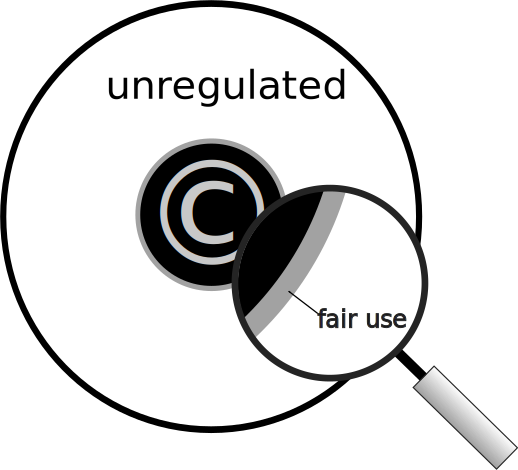
\includegraphics[width=0.4\linewidth,keepaspectratio=true]{images/1542.svg}}}}{[images/1542.svg not found]}
\end{center}
\addtocounter{figure}{-1}\caption{}
\end{figure}
\index{copyright!usage restrictions attached to|(}

  In real space, then, the possible uses of a book are divided into three
sorts: (1) unregulated uses, (2) regulated uses, and (3) regulated uses that
are nonetheless deemed «fair» regardless of the copyright owner's views.

\index{books!three types of uses of|)}\index{books!on Internet|(}\index{Internet!books on|(}\index{fair use!Internet burdens on}

 Enter the Internet—a distributed, digital network where every use
of a copyrighted work produces a copy.\footnote{
  I don't mean «nature» in the sense that it couldn't be different, but
rather that its present instantiation entails a copy. Optical networks
need not make copies of content they transmit, and a digital network
could be designed to delete anything it copies so that the same number
of copies remain.

} And because of this single, arbitrary feature of the design of a
digital network, the scope of category 1 changes dramatically. Uses
that before were presumptively unregulated are now presumptively
regulated. No longer is there a set of presumptively unregulated uses
that define a freedom associated with a copyrighted work. Instead,
each use is now subject to the copyright, because each use also makes
a copy—category 1 gets sucked into category 2. And those who
would defend the unregulated uses of copyrighted work must look
exclusively to category 3, fair uses, to bear the burden of this
shift.

\index{fair use|)}\index{copyright law!fair use and|)}

 So let's be very specific to make this general point clear. Before the
Internet, if you purchased a book and read it ten times, there would
be no plausible \emph{copyright}-{}related argument that
the copyright owner could make to control that use of her
book. Copyright law would have nothing to say about whether you read
the book once, ten times, or every
 night before you went to bed. None of those instances of
use—reading— could be regulated by copyright law because
none of those uses produced a copy.

\index{e-{}books|(}\index{derivative works!technological developments and|(}

 But the same book as an e-{}book is effectively governed by a different
set of rules. Now if the copyright owner says you may read the book
only once or only once a month, then \emph{copyright
law} would aid the copyright owner in exercising this degree
of control, because of the accidental feature of copyright law that
triggers its application upon there being a copy. Now if you read the
book ten times and the license says you may read it only five times,
then whenever you read the book (or any portion of it) beyond the
fifth time, you are making a copy of the book contrary to the
copyright owner's wish.

\begin{figure}[H]
\refstepcounter{figure}\label{fig-1551}\hyperlabel{fig-1551}%

\begin{center}
\imgexists{images/1551.svg}{{\centering \imgevalsize{images/1551.svg}{\includegraphics[width=0.4\linewidth,keepaspectratio=true]{images/1551.svg}}}}{[images/1551.svg not found]}
\end{center}
\addtocounter{figure}{-1}\caption{}
\end{figure}

 There are some people who think this makes perfect sense. My aim
just now is not to argue about whether it makes sense or not. My aim
is only to make clear the change. Once you see this point, a few other
points also become clear:


 First, making category 1 disappear is not anything any policy maker
ever intended. Congress did not think through the collapse of the
presumptively unregulated uses of copyrighted works. There is no
evidence at all that policy makers had this idea in mind when they
allowed our policy here to shift. Unregulated uses were an important
part of free culture before the Internet.

\index{copyright law!on republishing vs. transformation of original work|(}

 Second, this shift is especially troubling in the context of
transformative uses of creative content. Again, we can all understand
the wrong in commercial piracy. But the law now purports to regulate
\emph{any} transformation you make of creative work
using a machine. «Copy and paste» and «cut and paste» become
crimes. Tinkering with a story and releasing it to others exposes the
tinkerer to at least a requirement of justification.  However
troubling the expansion with respect to copying a particular work, it
is extraordinarily troubling with respect to transformative uses of
creative work.

\index{fair use!Internet burdens on|(}\index{copyright law!fair use and|(}\index{derivative works!fair use vs.|(}

 Third, this shift from category 1 to category 2 puts an extraordinary
  burden on category 3 («fair use») that fair use never before had to
bear.  If a copyright owner now tried to control how many times I
could read a book on-{}line, the natural response would be to argue that
this is a violation of my fair use rights. But there has never been
any litigation about whether I have a fair use right to read, because
before the Internet, reading did not trigger the application of
copyright law and hence the need for a fair use defense. The right to
read was effectively protected before because reading was not
regulated.

\index{copyright law!copies as core issue of|)}\index{Internet!copyright applicability altered by technology of|)}\index{technology!copyright intent altered by|)}\index{derivative works!technological developments and|)}
\index{copyright law!on republishing vs. transformation of original work|)}

 This point about fair use is totally ignored, even by advocates for
free culture. We have been cornered into arguing that our rights
depend upon fair use—never even addressing the earlier question
about the expansion in effective regulation. A thin protection
grounded in fair use makes sense when the vast majority of uses are
\emph{unregulated}. But when everything becomes
presumptively regulated, then the protections of fair use are not
enough.

\index{copyright!usage restrictions attached to|)}
\index{books!on Internet|)}\index{Internet!books on|)}\index{e-{}books|)}\index{fair use!Internet burdens on|)}\index{copyright law!fair use and|)}\index{derivative works!fair use vs.|)}
\index{Video Pipeline|(}\index{advertising|(}\index{film industry!trailer advertisements of|(}

 The case of Video Pipeline is a good example. Video Pipeline was
in the business of making «trailer» advertisements for movies available
to video stores. The video stores displayed the trailers as a way to sell
videos. Video Pipeline got the trailers from the film distributors, put
the trailers on tape, and sold the tapes to the retail stores.

\index{browsing}

 The company did this for about fifteen years. Then, in 1997, it began
to think about the Internet as another way to distribute these
previews.  The idea was to expand their «selling by sampling» technique by giving on-{}line stores the same ability to enable
«browsing.» Just as in a bookstore you can read a few pages of a book
before you buy the book, so, too, you would be able to sample a bit
from the movie on-{}line before you bought it.

\index{Disney, Inc.|(}\index{copyright law!fair use and}\index{copyright law!copies as core issue of|(}\index{fair use!legal intimidation tactics against|(}

 In 1998, Video Pipeline informed Disney and other film distributors
that it intended to distribute the trailers through the Internet
(rather than sending the tapes) to distributors of their videos. Two
years later, Disney told Video Pipeline to stop. The owner of Video
 Pipeline asked Disney to talk about the matter—he had built a
business on distributing this content as a way to help sell Disney
films; he had customers who depended upon his delivering this
content. Disney would agree to talk only if Video Pipeline stopped the
distribution immediately.  Video Pipeline thought it was within their
«fair use» rights to distribute the clips as they had. So they filed a
lawsuit to ask the court to declare that these rights were in fact
their rights.

\index{advertising|)}\index{film industry!trailer advertisements of|)}
\index{copyright!usage restrictions attached to|(}\index{copyright infringement lawsuits!willful infringement findings in|(}\index{willful infringement}

 Disney countersued—for \$100 million in damages. Those damages
were predicated upon a claim that Video Pipeline had «willfully
infringed» on Disney's copyright. When a court makes a finding of
willful infringement, it can award damages not on the basis of the
actual harm to the copyright owner, but on the basis of an amount set
in the statute. Because Video Pipeline had distributed seven hundred
clips of Disney movies to enable video stores to sell copies of those
movies, Disney was now suing Video Pipeline for \$100 million.


 Disney has the right to control its property, of course. But the video
stores that were selling Disney's films also had some sort of right to be
able to sell the films that they had bought from Disney. Disney's claim
in court was that the stores were allowed to sell the films and they were
permitted to list the titles of the films they were selling, but they were
not allowed to show clips of the films as a way of selling them without
Disney's permission.

\index{first-{}sale doctrine}

 Now, you might think this is a close case, and I think the courts
would consider it a close case. My point here is to map the change
that gives Disney this power. Before the Internet, Disney couldn't
really control how people got access to their content. Once a video
was in the marketplace, the «first-{}sale doctrine» would free the
seller to use the video as he wished, including showing portions of it
in order to engender sales of the entire movie video. But with the
Internet, it becomes possible for Disney to centralize control over
access to this content. Because each use of the Internet produces a
copy, use on the Internet becomes subject to the copyright owner's
control. The technology expands the scope of effective control,
because the technology builds a copy into every transaction.

\index{Video Pipeline|)}\index{Disney, Inc.|)}\index{copyright law!copies as core issue of|)}\index{fair use!legal intimidation tactics against|)}
\index{copyright!usage restrictions attached to|)}\index{copyright infringement lawsuits!willful infringement findings in|)}\index{Barnes \& Noble}\index{browsing}\index{market competition}

  No doubt, a potential is not yet an abuse, and so the potential for
control is not yet the abuse of control. Barnes \& Noble has the
right to say you can't touch a book in their store; property law gives
them that right.  But the market effectively protects against that
abuse. If Barnes \& Noble banned browsing, then consumers would
choose other bookstores.  Competition protects against the
extremes. And it may well be (my argument so far does not even
question this) that competition would prevent any similar danger when
it comes to copyright. Sure, publishers exercising the rights that
authors have assigned to them might try to regulate how many times you
read a book, or try to stop you from sharing the book with anyone. But
in a competitive market such as the book market, the dangers of this
happening are quite slight.


 Again, my aim so far is simply to map the changes that this changed
architecture enables. Enabling technology to enforce the control of
copyright means that the control of copyright is no longer defined by
balanced policy. The control of copyright is simply what private
owners choose. In some contexts, at least, that fact is harmless. But
in some contexts it is a recipe for disaster.


\section{Architecture and Law: Force}
\label{lawforce}\hyperlabel{lawforce}%

 The disappearance of unregulated uses would be change enough, but a
second important change brought about by the Internet magnifies its
significance. This second change does not affect the reach of copyright
regulation; it affects how such regulation is enforced.

\index{copyright law!technology as automatic enforcer of}\index{technology!copyright enforcement controlled by}

 In the world before digital technology, it was generally the law that
controlled whether and how someone was regulated by copyright law.
The law, meaning a court, meaning a judge: In the end, it was a human,
trained in the tradition of the law and cognizant of the balances that
tradition embraced, who said whether and how the law would restrict
your freedom.

\index{Casablanca}\index{Marx Brothers|(}\index{Warner Brothers|(}

 There's a famous story about a battle between the Marx Brothers
and Warner Brothers. The Marxes intended to make a parody of
 \emph{Casablanca}. Warner Brothers objected. They
wrote a nasty letter to the Marxes, warning them that there would be
serious legal consequences if they went forward with their
plan.\footnote{
  See David Lange, «Recognizing the Public Domain,» \emph{Law and
Contemporary Problems} 44 (1981): 172–73.

} 

 This led the Marx Brothers to respond in kind. They warned
Warner Brothers that the Marx Brothers «were brothers long before
you were.»\footnote{
  \index{Vaidhyanathan, Siva} Ibid. See also Vaidhyanathan, \emph{Copyrights and
Copywrongs}, 1–3.

} The Marx Brothers therefore owned the word
\emph{brothers}, and if Warner Brothers insisted on
trying to control \emph{Casablanca}, then the Marx
Brothers would insist on control over \emph{brothers}.


 An absurd and hollow threat, of course, because Warner Brothers,
like the Marx Brothers, knew that no court would ever enforce such a
silly claim. This extremism was irrelevant to the real freedoms anyone
(including Warner Brothers) enjoyed.

\index{books!on Internet|(}

 On the Internet, however, there is no check on silly rules, because on
the Internet, increasingly, rules are enforced not by a human but by a
machine: Increasingly, the rules of copyright law, as interpreted by
the copyright owner, get built into the technology that delivers
copyrighted content. It is code, rather than law, that rules. And the
problem with code regulations is that, unlike law, code has no
shame. Code would not get the humor of the Marx Brothers. The
consequence of that is not at all funny.

\index{Warner Brothers|)}
\index{Marx Brothers|)}\index{Adobe eBook Reader|(}

 Consider the life of my Adobe eBook Reader.


 An e-{}book is a book delivered in electronic form. An Adobe eBook is
not a book that Adobe has published; Adobe simply produces the
software that publishers use to deliver e-{}books. It provides the
technology, and the publisher delivers the content by using the
technology.

\begin{figure}[htbp]
\refstepcounter{figure}\label{fig-example-adobe-ebook-reader}\hyperlabel{fig-example-adobe-ebook-reader}%

\begin{center}
\imgexists{images/example-adobe-ebook-reader.png}{{\centering \imgevalsize{images/example-adobe-ebook-reader.png}{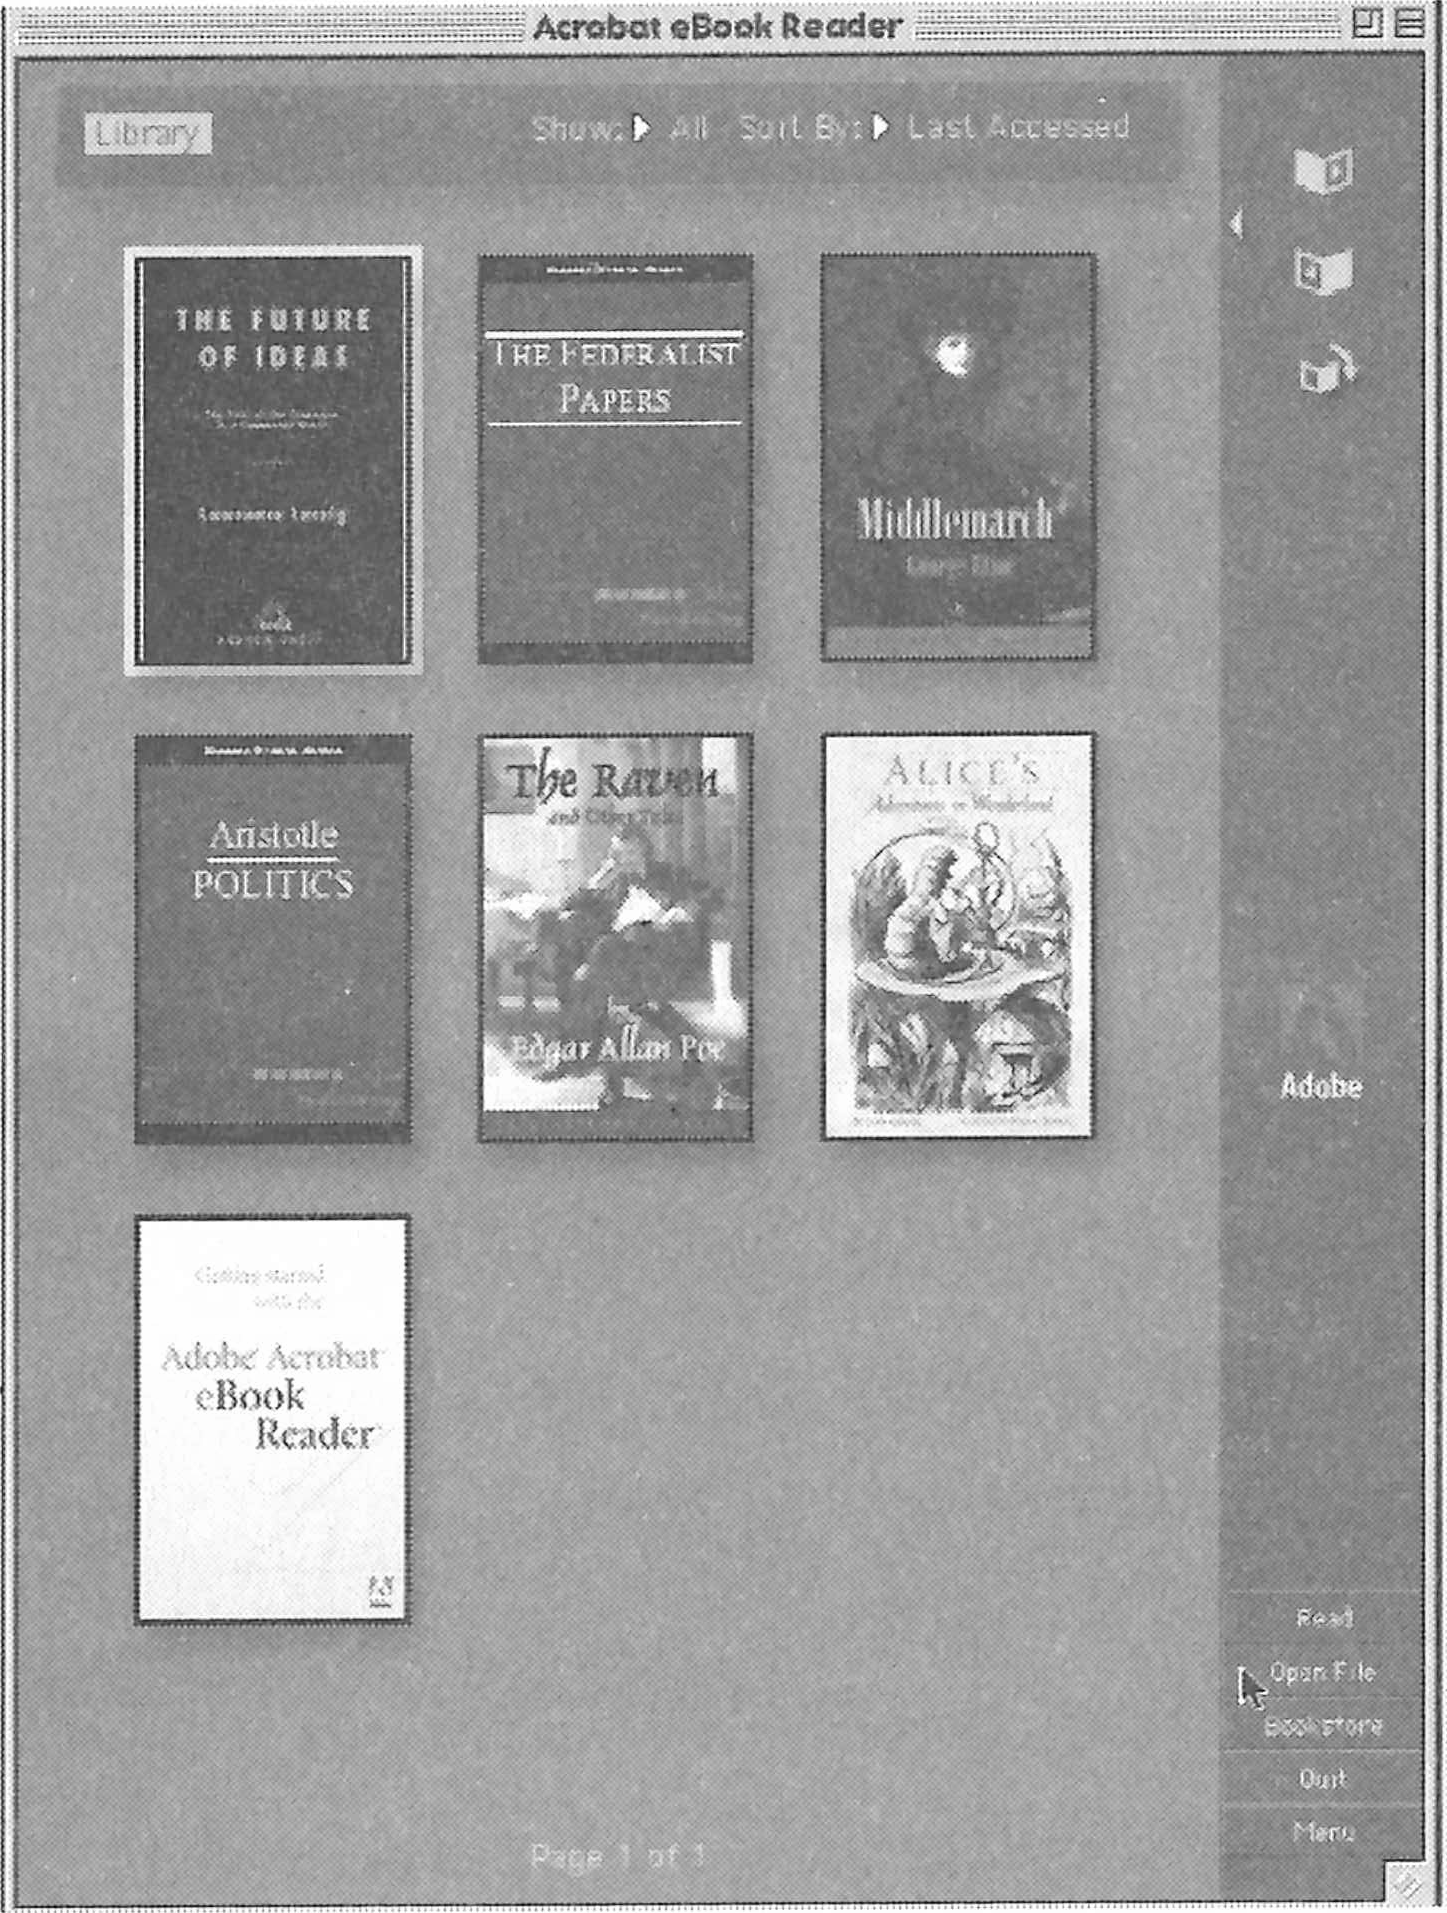
\includegraphics[width=0.5\linewidth,keepaspectratio=true]{images/example-adobe-ebook-reader.png}}}}{[images/example-{}adobe-{}ebook-{}reader.png not found]}
\end{center}
\addtocounter{figure}{-1}\caption{}
\end{figure}

 In figure
\ref{fig-example-adobe-ebook-reader} [\pageref{fig-example-adobe-ebook-reader}] is a picture of an old version of my Adobe eBook Reader.


 As you can see, I have a small collection of e-{}books within this
e-{}book library. Some of these books reproduce content that is in the
public domain: \emph{Middlemarch}, for example, is in
the public domain.  Some of them reproduce content that is not in the
public domain: My own book \emph{The Future of Ideas} is not yet within the public domain.  Consider
\emph{Middlemarch} first. If you click on my e-{}book
copy of
 \emph{Middlemarch}, you'll see a fancy cover, and then
a button at the bottom called Permissions.


 If you click on the Permissions button, you'll see a list of the
permissions that the publisher purports to grant with this book.

\begin{figure}[H]
\refstepcounter{figure}\label{fig-1612}\hyperlabel{fig-1612}%

\begin{center}
\imgexists{images/1612.png}{{\centering \imgevalsize{images/1612.png}{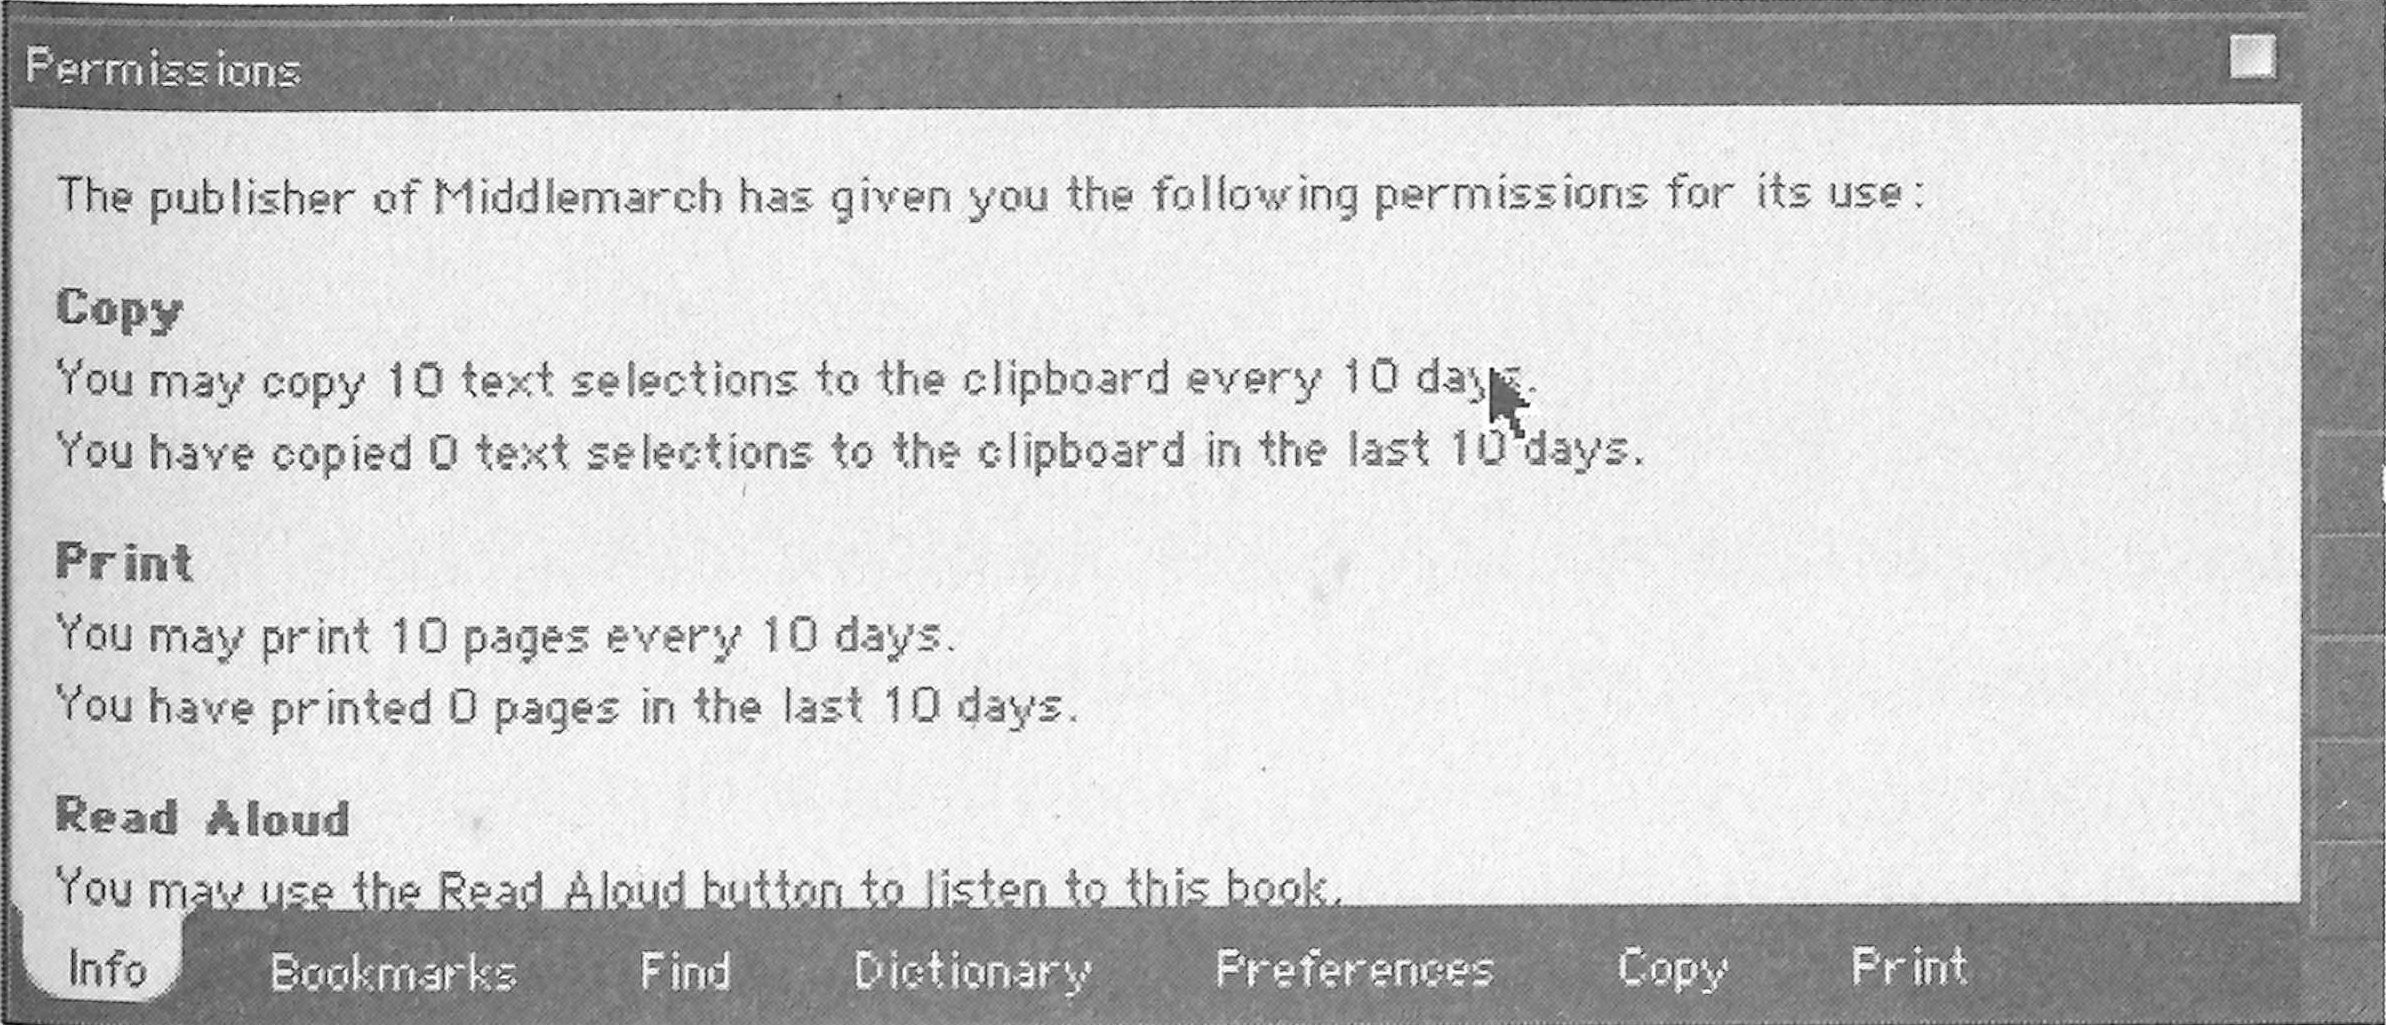
\includegraphics[width=0.5\linewidth,keepaspectratio=true]{images/1612.png}}}}{[images/1612.png not found]}
\end{center}
\addtocounter{figure}{-1}\caption{}
\end{figure}

  According to my eBook Reader, I have the permission to copy to the
clipboard of the computer ten text selections every ten days. (So far,
I've copied no text to the clipboard.)  I also have the permission to
print ten pages from the book every ten days. Lastly, I have the
permission to use the Read Aloud button to hear \emph{Middlemarch} read aloud through the computer.

\index{Aristotle}\index{Politics, (Aristotle)}

 Here's the e-{}book for another work in the public domain (including the
translation): Aristotle's \emph{Politics}.

\begin{figure}[H]
\refstepcounter{figure}\label{fig-1621}\hyperlabel{fig-1621}%

\begin{center}
\imgexists{images/aristotele-ebook.png}{{\centering \imgevalsize{images/aristotele-ebook.png}{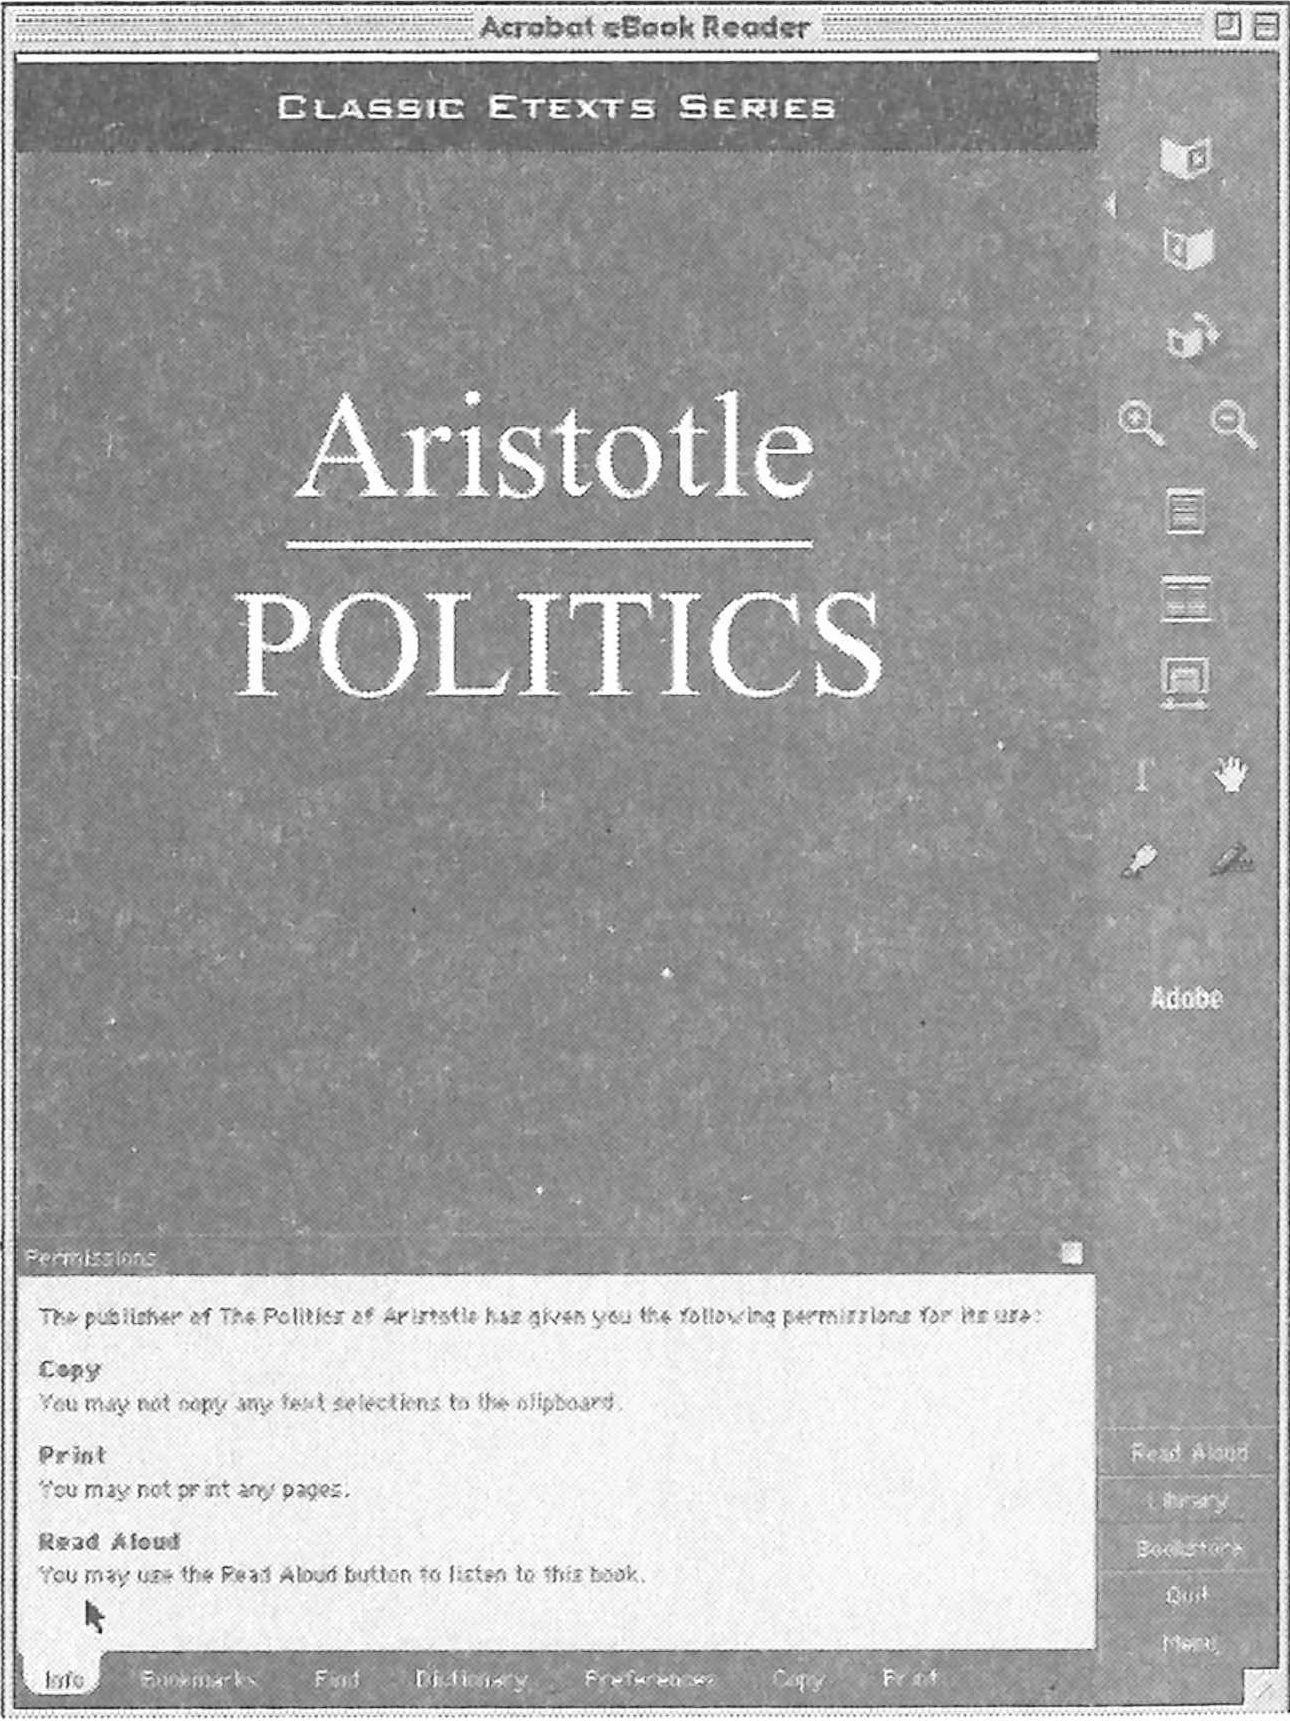
\includegraphics[width=0.5\linewidth,keepaspectratio=true]{images/aristotele-ebook.png}}}}{[images/aristotele-{}ebook.png not found]}
\end{center}
\addtocounter{figure}{-1}\caption{}
\end{figure}

 According to its permissions, no printing or copying is permitted
at all. But fortunately, you can use the Read Aloud button to hear
the book.

\begin{figure}[H]
\refstepcounter{figure}\label{fig-1622}\hyperlabel{fig-1622}%

\begin{center}
\imgexists{images/1622.png}{{\centering \imgevalsize{images/1622.png}{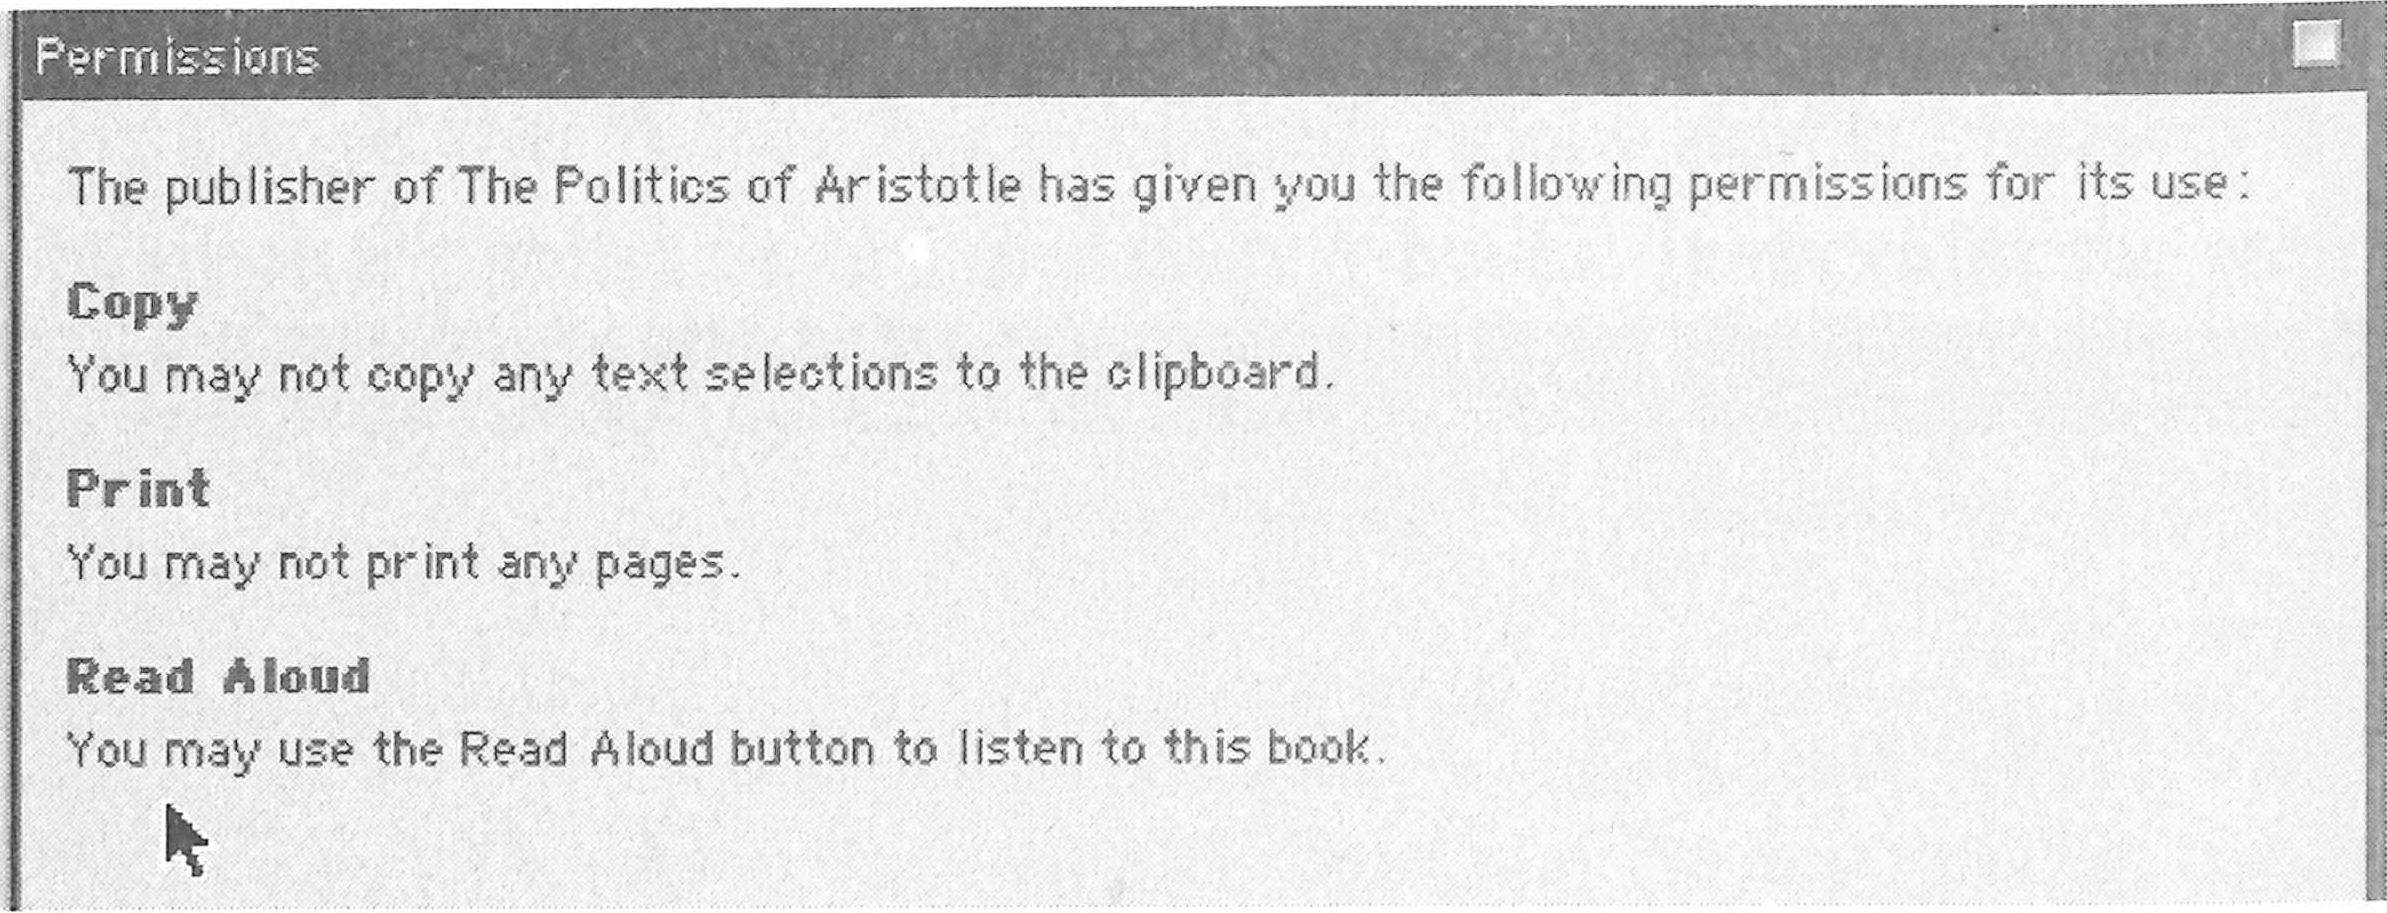
\includegraphics[width=0.5\linewidth,keepaspectratio=true]{images/1622.png}}}}{[images/1622.png not found]}
\end{center}
\addtocounter{figure}{-1}\caption{}
\end{figure}
\index{Future of Ideas, The (Lessig)}\index{Lessig, Lawrence}

 Finally (and most embarrassingly), here are the permissions for the
original e-{}book version of my last book, \emph{The Future of
Ideas}:

\begin{figure}[H]
\refstepcounter{figure}\label{fig-1631}\hyperlabel{fig-1631}%

\begin{center}
\imgexists{images/1631.png}{{\centering \imgevalsize{images/1631.png}{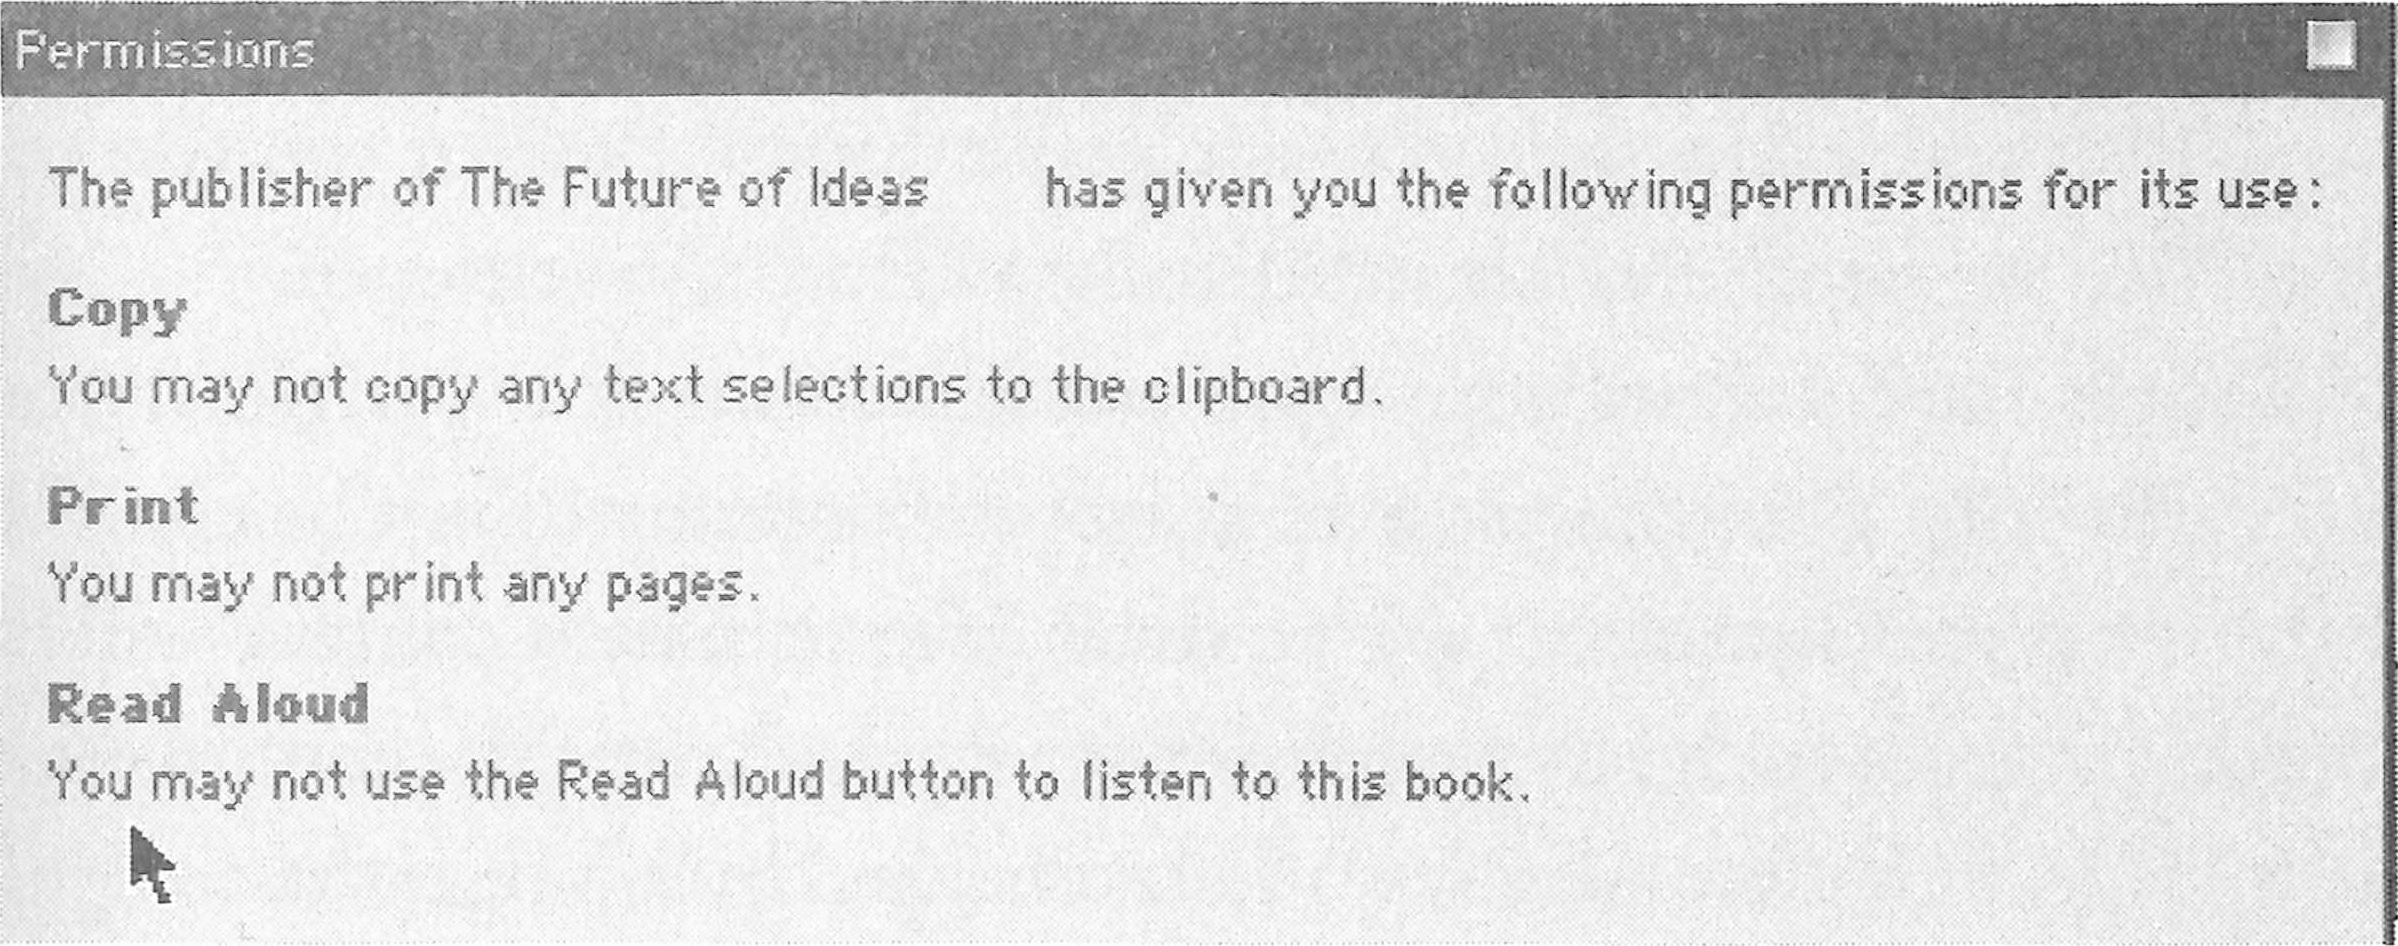
\includegraphics[width=0.5\linewidth,keepaspectratio=true]{images/1631.png}}}}{[images/1631.png not found]}
\end{center}
\addtocounter{figure}{-1}\caption{}
\end{figure}

 No copying, no printing, and don't you dare try to listen to this book!


 Now, the Adobe eBook Reader calls these controls
«permissions»— as if the publisher has the power to control how
you use these works.  For works under copyright, the copyright owner
certainly does have the power—up to the limits of the copyright
law. But for work not under copyright, there is no such copyright
power.\footnote{
  In principle, a contract might impose a requirement on me. I might,
for example, buy a book from you that includes a contract that says I
will read it only three times, or that I promise to read it three
times. But that obligation (and the limits for creating that
obligation) would come from the contract, not from copyright law, and
the obligations of contract would not necessarily pass to anyone who
subsequently acquired the book.

} When my e-{}book of \emph{Middlemarch} says I have the
permission to copy only ten text selections into the memory every ten
days, what that really means is that the eBook Reader has enabled the
publisher to control how I use the book on my computer, far beyond the
control that the law would enable.


 The control comes instead from the code—from the technology
within which the e-{}book «lives.» Though the e-{}book says that these are
permissions, they are not the sort of «permissions» that most of us
deal with. When a teenager gets «permission» to stay out till
midnight, she knows (unless she's Cinderella) that she can stay out
till 2 A.M., but will suffer a punishment if she's caught. But when
the Adobe eBook Reader says I have the permission to make ten copies
of the text into the computer's memory, that means that after I've
made ten copies, the computer will not make any more. The same with
the printing restrictions: After ten pages, the eBook Reader will not
print any more pages.  It's the same with the silly restriction that
says that you can't use the Read Aloud button to read my book
aloud—it's not that the company will sue you if you do; instead,
if you push the Read Aloud button with my book, the machine simply
won't read aloud.

\index{Marx Brothers}\index{Warner Brothers}

  These are \emph{controls}, not permissions. Imagine a
world where the Marx Brothers sold word processing software that, when
you tried to type «Warner Brothers,» erased «Brothers» from the
sentence.


 This is the future of copyright law: not so much copyright
\emph{law} as copyright \emph{code}. The
controls over access to content will not be controls that are ratified
by courts; the controls over access to content will be controls that
are coded by programmers. And whereas the controls that are built into
the law are always to be checked by a judge, the controls that are
built into the technology have no similar built-{}in check.


 How significant is this? Isn't it always possible to get around the
controls built into the technology? Software used to be sold with
technologies that limited the ability of users to copy the software,
but those were trivial protections to defeat. Why won't it be trivial
to defeat these protections as well?


 We've only scratched the surface of this story. Return to the Adobe
eBook Reader.

\index{Alice's Adventures in Wonderland (Carroll)|(}\index{public domain!e-{}book restrictions on|(}

 Early in the life of the Adobe eBook Reader, Adobe suffered a public
relations nightmare. Among the books that you could download for free
on the Adobe site was a copy of \emph{Alice's Adventures in
Wonderland}.  This wonderful book is in the public
domain. Yet when you clicked on Permissions for that book, you got the
following report:

\begin{figure}[H]
\refstepcounter{figure}\label{fig-1641}\hyperlabel{fig-1641}%

\begin{center}
\imgexists{images/1641.png}{{\centering \imgevalsize{images/1641.png}{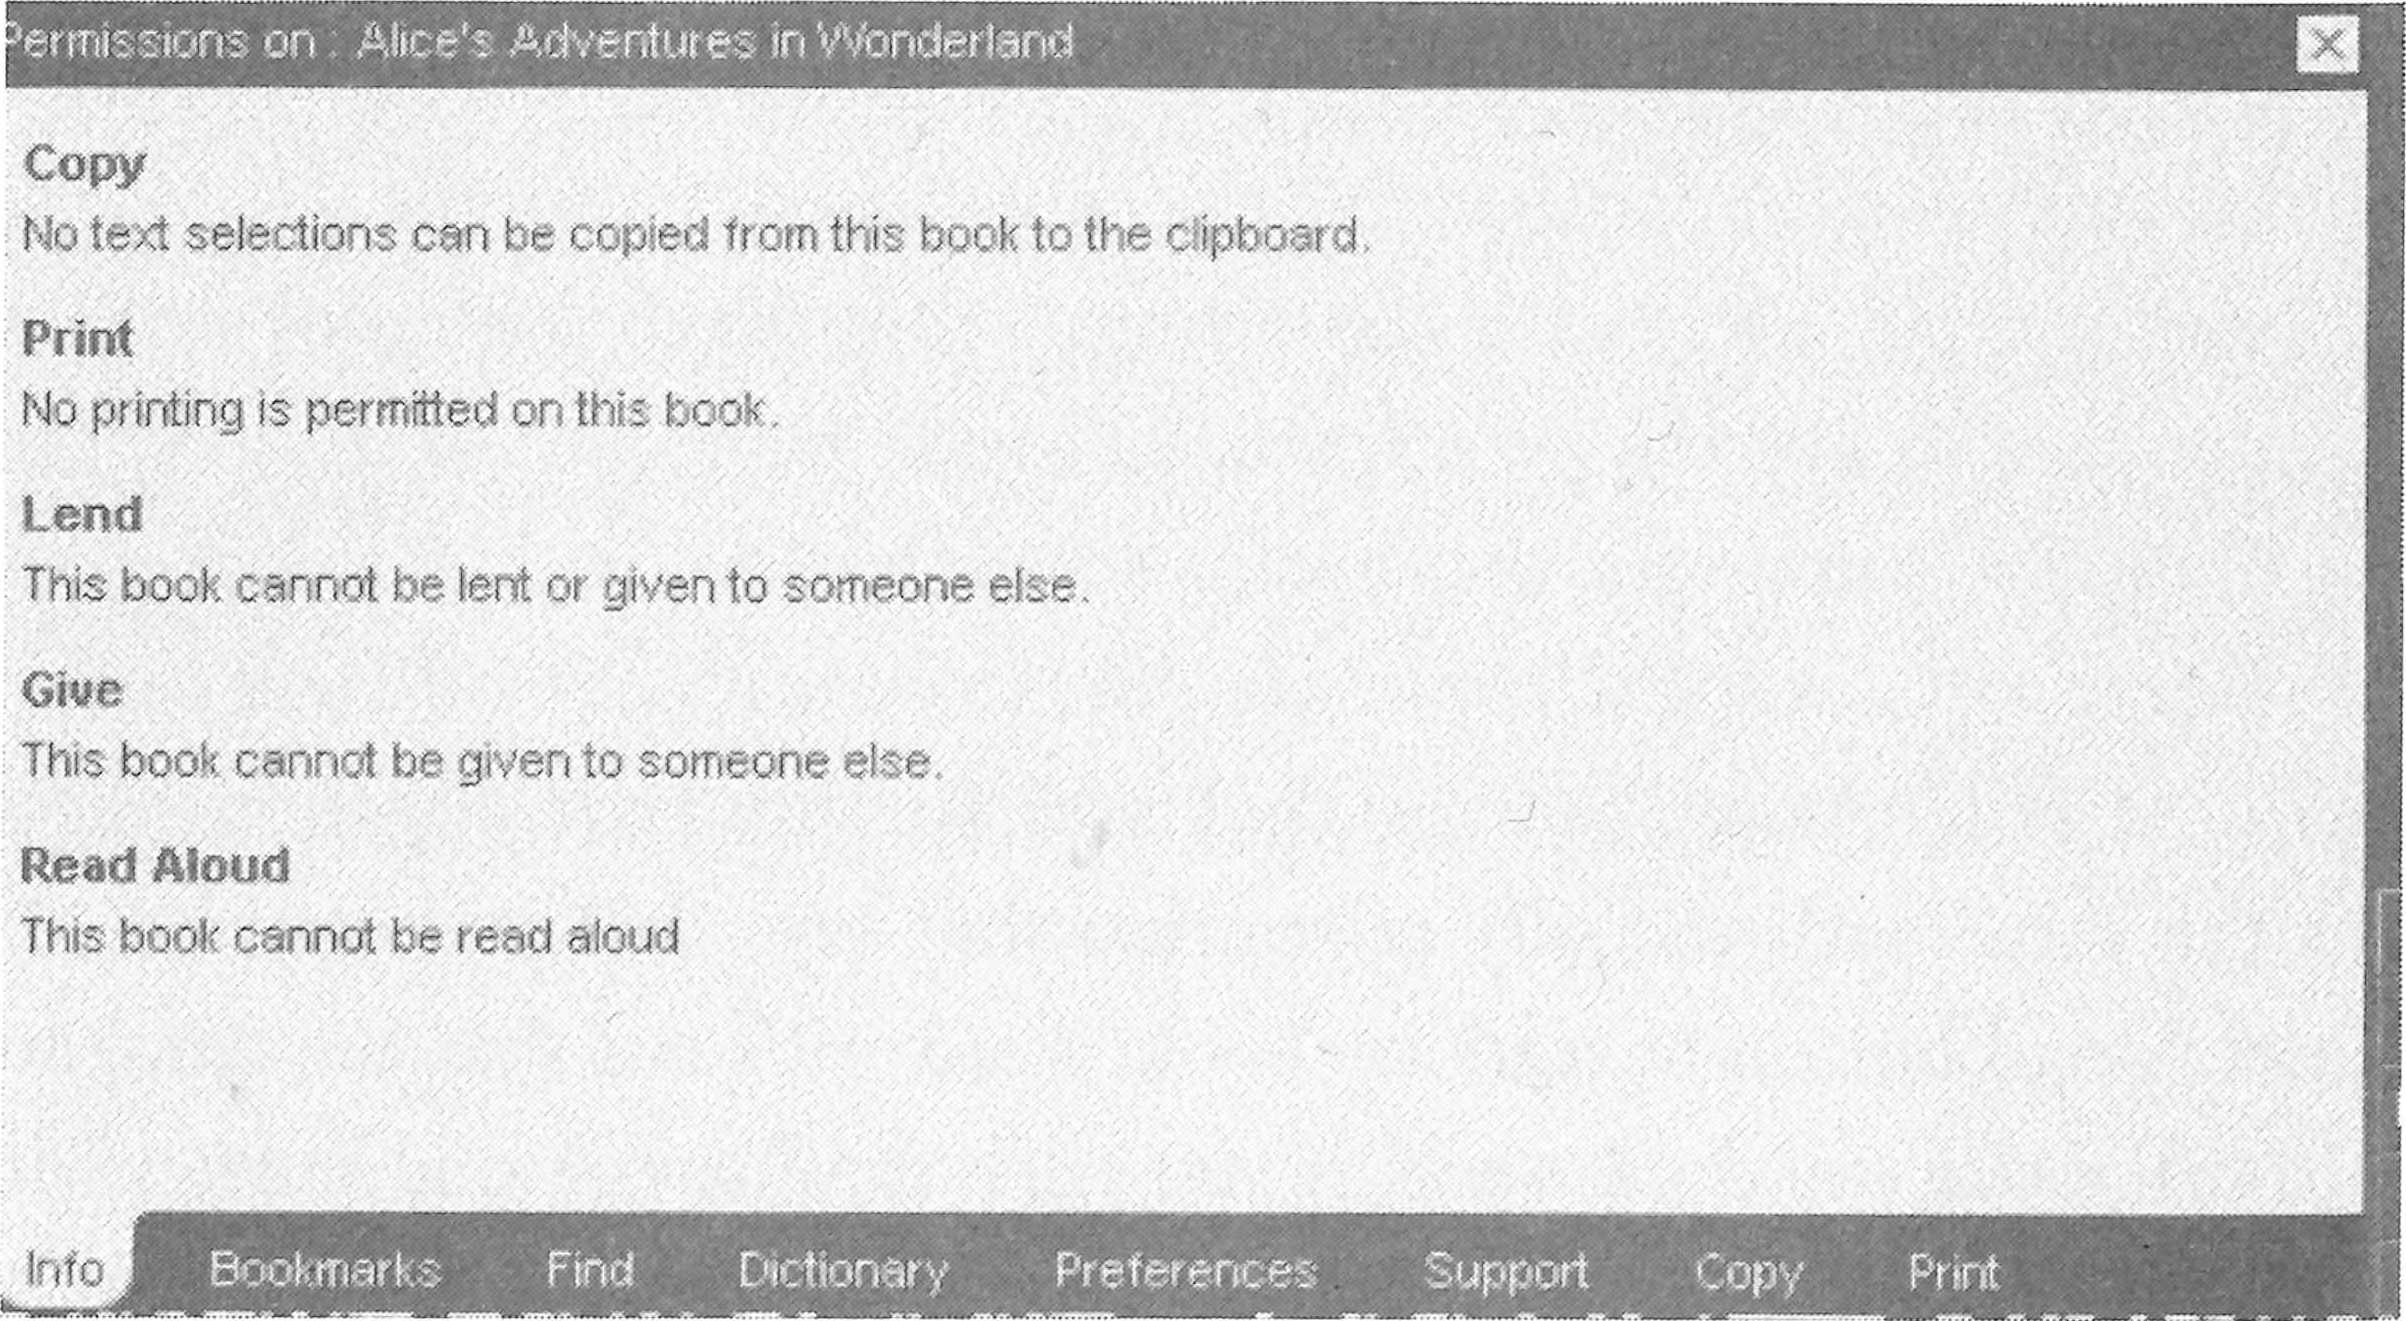
\includegraphics[width=0.5\linewidth,keepaspectratio=true]{images/1641.png}}}}{[images/1641.png not found]}
\end{center}
\addtocounter{figure}{-1}\caption{}
\end{figure}

 Here was a public domain children's book that you were not allowed to
copy, not allowed to lend, not allowed to give, and, as the
«permissions» indicated, not allowed to «read aloud»!


 The public relations nightmare attached to that final permission.
For the text did not say that you were not permitted to use the Read
Aloud button; it said you did not have the permission to read the book
aloud. That led some people to think that Adobe was restricting the
right of parents, for example, to read the book to their children, which
seemed, to say the least, absurd.


 Adobe responded quickly that it was absurd to think that it was trying
to restrict the right to read a book aloud. Obviously it was only
restricting the ability to use the Read Aloud button to have the book
read aloud. But the question Adobe never did answer is this: Would
Adobe thus agree that a consumer was free to use software to hack
around the restrictions built into the eBook Reader? If some company
(call it Elcomsoft) developed a program to disable the technological
protection built into an Adobe eBook so that a blind person, say,
could use a computer to read the book aloud, would Adobe agree that
such a use of an eBook Reader was fair? Adobe didn't answer because
the answer, however absurd it might seem, is no.

\index{Alice's Adventures in Wonderland (Carroll)|)}\index{public domain!e-{}book restrictions on|)}

 The point is not to blame Adobe. Indeed, Adobe is among the most
innovative companies developing strategies to balance open access to
content with incentives for companies to innovate. But Adobe's
technology enables control, and Adobe has an incentive to defend this
control.  That incentive is understandable, yet what it creates is
often crazy.

\index{Adobe eBook Reader|)}
\index{books!on Internet|)}

 To see the point in a particularly absurd context, consider a favorite
story of mine that makes the same point.

\index{Aibo robotic dog|(}\index{robotic dog|(}\index{Sony!Aibo robotic dog produced by|(}

 Consider the robotic dog made by Sony named «Aibo.» The Aibo
learns tricks, cuddles, and follows you around. It eats only electricity
and that doesn't leave that much of a mess (at least in your house).


 The Aibo is expensive and popular. Fans from around the world
have set up clubs to trade stories. One fan in particular set up a Web
site to enable information about the Aibo dog to be shared. This fan set
 up aibopet.com (and aibohack.com, but that resolves to the same site),
and on that site he provided information about how to teach an Aibo
to do tricks in addition to the ones Sony had taught it.


 «Teach» here has a special meaning. Aibos are just cute computers.
You teach a computer how to do something by programming it
differently.  So to say that aibopet.com was giving information about
how to teach the dog to do new tricks is just to say that aibopet.com
was giving information to users of the Aibo pet about how to hack
their computer «dog» to make it do new tricks (thus, aibohack.com).

\index{hacks}

 If you're not a programmer or don't know many programmers, the word
\emph{hack} has a particularly unfriendly
connotation. Nonprogrammers hack bushes or weeds. Nonprogrammers in
horror movies do even worse. But to programmers, or coders, as I call
them, \emph{hack} is a much more positive
term. \emph{Hack} just means code that enables the
program to do something it wasn't originally intended or enabled to
do. If you buy a new printer for an old computer, you might find the
old computer doesn't run, or «drive,» the printer. If you discovered
that, you'd later be happy to discover a hack on the Net by someone
who has written a driver to enable the computer to drive the printer
you just bought.


 Some hacks are easy. Some are unbelievably hard. Hackers as a
community like to challenge themselves and others with increasingly
difficult tasks. There's a certain respect that goes with the talent to hack
well. There's a well-{}deserved respect that goes with the talent to hack
ethically.


 The Aibo fan was displaying a bit of both when he hacked the program
and offered to the world a bit of code that would enable the Aibo to
dance jazz. The dog wasn't programmed to dance jazz. It was a clever
bit of tinkering that turned the dog into a more talented creature
than Sony had built.

\index{Sony!Aibo robotic dog produced by|)}
\index{robotic dog|)}\index{Aibo robotic dog|)}
 I've told this story in many contexts, both inside and outside the
United States. Once I was asked by a puzzled member of the audience,
is it permissible for a dog to dance jazz in the United States? We
forget that stories about the backcountry still flow across much of
the
  world. So let's just be clear before we continue: It's not a crime
anywhere (anymore) to dance jazz. Nor is it a crime to teach your dog
to dance jazz. Nor should it be a crime (though we don't have a lot to
go on here) to teach your robot dog to dance jazz. Dancing jazz is a
completely legal activity. One imagines that the owner of aibopet.com
thought, \emph{What possible problem could there be with teaching
a robot dog to dance?} 
\index{Microsoft!government case against}

 Let's put the dog to sleep for a minute, and turn to a pony show—
not literally a pony show, but rather a paper that a Princeton academic
named Ed Felten prepared for a conference. This Princeton academic
is well known and respected. He was hired by the government in the
Microsoft case to test Microsoft's claims about what could and could
not be done with its own code. In that trial, he demonstrated both his
brilliance and his coolness. Under heavy badgering by Microsoft
lawyers, Ed Felten stood his ground. He was not about to be bullied
into being silent about something he knew very well.


 But Felten's bravery was really tested in April 2001.\footnote{
  See Pamela Samuelson, «Anticircumvention Rules: Threat to Science,» \emph{Science} 293 (2001): 2028; Brendan I. Koerner, «Play Dead: Sony Muzzles
the Techies Who Teach a Robot Dog New Tricks,» \emph{American Prospect},
January 2002; «Court Dismisses Computer Scientists' Challenge to
DMCA,» \emph{Intellectual Property Litigation Reporter}, 11 December 2001; Bill
Holland, «Copyright Act Raising Free-{}Speech Concerns,» \emph{Billboard},
May 2001; Janelle Brown, «Is the RIAA Running Scared?» Salon.com,
April  2001; Electronic Frontier Foundation, «Frequently Asked 
Questions about \emph{Felten and USENIX} v. \emph{RIAA} Legal Case,» available at 
\href{http://free-culture.cc/notes/}{link \#27}.
\index{Electronic Frontier Foundation} 
} He and a group of colleagues were working on a paper to be submitted
at conference.  The paper was intended to describe the weakness in an
encryption system being developed by the Secure Digital Music
Initiative as a technique to control the distribution of music.


 The SDMI coalition had as its goal a technology to enable content
owners to exercise much better control over their content than the
Internet, as it originally stood, granted them. Using encryption, SDMI
hoped to develop a standard that would allow the content owner to say
«this music cannot be copied,» and have a computer respect that
command.  The technology was to be part of a «trusted system» of
control that would get content owners to trust the system of the
Internet much more.


 When SDMI thought it was close to a standard, it set up a competition.
In exchange for providing contestants with the code to an
SDMI-{}encrypted bit of content, contestants were to try to crack it
and, if they did, report the problems to the consortium.


  Felten and his team figured out the encryption system quickly. He and
the team saw the weakness of this system as a type: Many encryption
systems would suffer the same weakness, and Felten and his team
thought it worthwhile to point this out to those who study encryption.


 Let's review just what Felten was doing. Again, this is the United
States. We have a principle of free speech. We have this principle not
just because it is the law, but also because it is a really great
idea. A strongly protected tradition of free speech is likely to
encourage a wide range of criticism. That criticism is likely, in
turn, to improve the systems or people or ideas criticized.


 What Felten and his colleagues were doing was publishing a paper
describing the weakness in a technology. They were not spreading free
music, or building and deploying this technology. The paper was an
academic essay, unintelligible to most people. But it clearly showed the
weakness in the SDMI system, and why SDMI would not, as presently
constituted, succeed.

\index{Aibo robotic dog|(}\index{robotic dog|(}\index{Sony!Aibo robotic dog produced by|(}

 What links these two, aibopet.com and Felten, is the letters they
then received. Aibopet.com received a letter from Sony about the
aibopet.com hack. Though a jazz-{}dancing dog is perfectly legal, Sony
wrote:

\begin{quote}

 Your site contains information providing the means to circumvent
AIBO-{}ware's copy protection protocol constituting a violation of the
anti-{}circumvention provisions of the Digital Millennium Copyright Act.


\end{quote}
\index{Sony!Aibo robotic dog produced by|)}
\index{robotic dog|)}\index{Aibo robotic dog|)}
 And though an academic paper describing the weakness in a system
of encryption should also be perfectly legal, Felten received a letter
from an RIAA lawyer that read:

\begin{quote}

 Any  disclosure of information gained from participating in the
 Public Challenge would be outside the scope of activities permitted by
the Agreement and could subject you and your research team to actions
under the Digital Millennium Copyright Act («DMCA»).


\end{quote}

 In both cases, this weirdly Orwellian law was invoked to control the
spread of information. The Digital Millennium Copyright Act made
spreading such information an offense.


 The DMCA was enacted as a response to copyright owners' first fear
about cyberspace. The fear was that copyright control was effectively
dead; the response was to find technologies that might compensate.
These new technologies would be copyright protection
technologies— technologies to control the replication and
distribution of copyrighted material. They were designed as
\emph{code} to modify the original
\emph{code} of the Internet, to reestablish some
protection for copyright owners.


 The DMCA was a bit of law intended to back up the protection of this
code designed to protect copyrighted material. It was, we could say,
\emph{legal code} intended to buttress
\emph{software code} which itself was intended to
support the \emph{legal code of copyright}.


 But the DMCA was not designed merely to protect copyrighted works to
the extent copyright law protected them. Its protection, that is, did
not end at the line that copyright law drew. The DMCA regulated
devices that were designed to circumvent copyright protection
measures. It was designed to ban those devices, whether or not the use
of the copyrighted material made possible by that circumvention would
have been a copyright violation.

\index{Aibo robotic dog}\index{robotic dog}\index{Sony!Aibo robotic dog produced by}

 Aibopet.com and Felten make the point. The Aibo hack circumvented a
copyright protection system for the purpose of enabling the dog to
dance jazz. That enablement no doubt involved the use of copyrighted
material. But as aibopet.com's site was noncommercial, and the use did
not enable subsequent copyright infringements, there's no doubt that
aibopet.com's hack was fair use of Sony's copyrighted material. Yet
fair use is not a defense to the DMCA. The question is not whether the
 use of the copyrighted material was a copyright violation. The question
is whether a copyright protection system was circumvented.


 The threat against Felten was more attenuated, but it followed the
same line of reasoning. By publishing a paper describing how a
copyright protection system could be circumvented, the RIAA lawyer
suggested, Felten himself was distributing a circumvention technology.
Thus, even though he was not himself infringing anyone's copyright,
his academic paper was enabling others to infringe others' copyright.

\index{Rogers, Fred}\index{cassette recording!VCRs|(}

 The bizarreness of these arguments is captured in a cartoon drawn in
1981 by Paul Conrad. At that time, a court in California had held that
the VCR could be banned because it was a copyright-{}infringing
technology: It enabled consumers to copy films without the permission
of the copyright owner. No doubt there were uses of the technology
that were legal: Fred Rogers, aka «\emph{Mr. Rogers},» for example, had testified in that case that he wanted people to feel
free to tape Mr. Rogers' Neighborhood.
\index{Conrad, Paul} 
\begin{quote}

 Some public stations, as well as commercial stations, program the
«Neighborhood» at hours when some children cannot use it. I think that
it's a real service to families to be able to record such programs and
show them at appropriate times. I have always felt that with the
advent of all of this new technology that allows people to tape the
«Neighborhood» off-{}the-{}air, and I'm speaking for the «Neighborhood» because that's what I produce, that they then become much more active
in the programming of their family's television life. Very frankly, I
am opposed to people being programmed by others. My whole approach in
broadcasting has always been «You are an important person just the way
you are. You can make healthy decisions.» Maybe I'm going on too long,
but I just feel that anything that allows a person to be more active
in the control of his or her life, in a healthy way, is
important.\footnote{
  \index{cassette recording!VCRs} \emph{Sony Corporation of America} v. \emph{Universal City Studios, Inc}., 464 U.S. 417,
455 fn. 27 (1984). Rogers never changed his view about the VCR. See
James Lardner, \emph{Fast Forward: Hollywood, the Japanese, and the Onslaught of
the VCR} (New York: W. W. Norton, 1987), 270–71.
\index{Rogers, Fred} 
} 

\end{quote}

  Even though there were uses that were legal, because there were
some uses that were illegal, the court held the companies producing
the VCR responsible.


 This led Conrad to draw the cartoon in figure
\ref{fig-1711-vcr-handgun-cartoonfig} [\pageref{fig-1711-vcr-handgun-cartoonfig}], which we can adopt to the
DMCA.
\index{Conrad, Paul} 

 No argument I have can top this picture, but let me try to get close.

\begin{figure}[htbp]
\refstepcounter{figure}\label{fig-1711-vcr-handgun-cartoonfig}\hyperlabel{fig-1711-vcr-handgun-cartoonfig}%

\begin{center}
\imgexists{images/vcr-comic.png}{{\centering \imgevalsize{images/vcr-comic.png}{\includegraphics[width=0.65\linewidth,keepaspectratio=true]{images/vcr-comic.png}}}}{[images/vcr-{}comic.png not found]}
\end{center}
\addtocounter{figure}{-1}\caption{— On which item have the courts ruled that manufacturers and
retailers be held responsible for having supplied the
equipment?}
\end{figure}

 The anticircumvention provisions of the DMCA target copyright
circumvention technologies. Circumvention technologies can be used for
different ends. They can be used, for example, to enable massive
pirating of copyrighted material—a bad end. Or they can be used
to enable the use of particular copyrighted materials in ways that
would be considered fair use—a good end.

\index{handguns|(}

 A handgun can be used to shoot a police officer or a child. Most
 would agree such a use is bad. Or a handgun can be used for target
practice or to protect against an intruder. At least some would say that
such a use would be good. It, too, is a technology that has both good
and bad uses.

\index{Conrad, Paul}

 The obvious point of Conrad's cartoon is the weirdness of a world
where guns are legal, despite the harm they can do, while VCRs (and
circumvention technologies) are illegal. Flash: \emph{No one ever
died from copyright circumvention}. Yet the law bans circumvention
technologies absolutely, despite the potential that they might do some
good, but permits guns, despite the obvious and tragic harm they do.

\index{handguns|)}
\index{cassette recording!VCRs|)}
\index{Aibo robotic dog}\index{robotic dog}\index{Sony!Aibo robotic dog produced by}

 The Aibo and RIAA examples demonstrate how copyright owners are
changing the balance that copyright law grants. Using code, copyright
owners restrict fair use; using the DMCA, they punish those who would
attempt to evade the restrictions on fair use that they impose through
code. Technology becomes a means by which fair use can be erased; the
law of the DMCA backs up that erasing.


 This is how \emph{code} becomes
\emph{law}. The controls built into the technology of
copy and access protection become rules the violation of which is also
a violation of the law. In this way, the code extends the
law—increasing its regulation, even if the subject it regulates
(activities that would otherwise plainly constitute fair use) is
beyond the reach of the law. Code becomes law; code extends the law;
code thus extends the control that copyright owners effect—at
least for those copyright holders with the lawyers who can write the
nasty letters that Felten and aibopet.com received.


 There is one final aspect of the interaction between architecture and
law that contributes to the force of copyright's regulation. This is
the ease with which infringements of the law can be detected. For
contrary to the rhetoric common at the birth of cyberspace that on the
Internet, no one knows you're a dog, increasingly, given changing
technologies deployed on the Internet, it is easy to find the dog who
committed a legal wrong. The technologies of the Internet are open to
snoops as well as sharers, and the snoops are increasingly good at
tracking down the identity of those who violate the rules.


   For example, imagine you were part of a \emph{Star Trek} fan club. You
gathered every month to share trivia, and maybe to enact a kind of fan
fiction about the show. One person would play Spock, another, Captain
Kirk. The characters would begin with a plot from a real story, then
simply continue it.\footnote{
  For an early and prescient analysis, see Rebecca Tushnet, «Legal Fictions,
Copyright, Fan Fiction, and a New Common Law,» \emph{Loyola of Los Angeles
Entertainment Law Journal} 17 (1997): 651.

} 

 Before the Internet, this was, in effect, a totally unregulated
activity.  No matter what happened inside your club room, you would
never be interfered with by the copyright police. You were free in
that space to do as you wished with this part of our culture. You were
allowed to build on it as you wished without fear of legal control.

\index{bots}

 But if you moved your club onto the Internet, and made it generally
available for others to join, the story would be very different. Bots
scouring the Net for trademark and copyright infringement would
quickly find your site. Your posting of fan fiction, depending upon
the ownership of the series that you're depicting, could well inspire
a lawyer's threat. And ignoring the lawyer's threat would be extremely
costly indeed.  The law of copyright is extremely efficient. The
penalties are severe, and the process is quick.


 This change in the effective force of the law is caused by a change
in the ease with which the law can be enforced. That change too shifts
the law's balance radically. It is as if your car transmitted the speed at
which you traveled at every moment that you drove; that would be just
one step before the state started issuing tickets based upon the data you
transmitted. That is, in effect, what is happening here.


\section{Market: Concentration}
\label{marketconcentration}\hyperlabel{marketconcentration}%

 So copyright's duration has increased dramatically—tripled in
the past thirty years. And copyright's scope has increased as
well—from regulating only publishers to now regulating just
about everyone. And copyright's reach has changed, as every action
becomes a copy and hence presumptively regulated. And as technologists
find better ways
 to control the use of content, and as copyright is increasingly
enforced through technology, copyright's force changes, too. Misuse is
easier to find and easier to control. This regulation of the creative
process, which began as a tiny regulation governing a tiny part of the
market for creative work, has become the single most important
regulator of creativity there is. It is a massive expansion in the
scope of the government's control over innovation and creativity; it
would be totally unrecognizable to those who gave birth to copyright's
control.


 Still, in my view, all of these changes would not matter much if it
weren't for one more change that we must also consider. This is a
change that is in some sense the most familiar, though its significance
and scope are not well understood. It is the one that creates precisely the
reason to be concerned about all the other changes I have described.


 This is the change in the concentration and integration of the media.
In the past twenty years, the nature of media ownership has undergone
a radical alteration, caused by changes in legal rules governing the
media.  Before this change happened, the different forms of media were
owned by separate media companies. Now, the media is increasingly
owned by only a few companies. Indeed, after the changes that the FCC
announced in June 2003, most expect that within a few years, we will
live in a world where just three companies control more than 85 percent
of the media.


 These changes are of two sorts: the scope of concentration, and its
nature.

\index{cable television}\index{BMG}\index{EMI}\index{McCain, John}\index{Universal Music Group}\index{Warner Music Group}

 Changes in scope are the easier ones to describe. As Senator John
McCain summarized the data produced in the FCC's review of media
ownership, «five companies control 85 percent of our media sources.»\footnote{
  FCC Oversight: Hearing Before the Senate Commerce, Science and
Transportation Committee, 108th Cong., 1st sess. (22 May 2003)
(statement of Senator John McCain).  
} The five recording labels of Universal Music Group, BMG, Sony Music
Entertainment, Warner Music Group, and EMI control 84.8 percent of the
U.S. music market.\footnote{
  Lynette Holloway, «Despite a Marketing Blitz, CD Sales Continue to
Slide,» \emph{New York Times}, 23 December 2002.

} The «five largest cable companies pipe
programming to 74 percent of the cable subscribers nationwide.»\footnote{
  Molly Ivins, «Media Consolidation Must Be Stopped,» \emph{Charleston Gazette},
31 May 2003.

} 

 The story with radio is even more dramatic. Before deregulation,
the nation's largest radio broadcasting conglomerate owned fewer than
 seventy-{}five stations. Today \emph{one} company owns
more than 1,200 stations.  During that period of consolidation, the
total number of radio owners dropped by 34 percent. Today, in most
markets, the two largest broadcasters control 74 percent of that
market's revenues. Overall, just four companies control 90 percent of
the nation's radio advertising revenues.

\index{cable television}

 Newspaper ownership is becoming more concentrated as well.  Today,
there are six hundred fewer daily newspapers in the United States than
there were eighty years ago, and ten companies control half of the
nation's circulation. There are twenty major newspaper publishers in
the United States. The top ten film studios receive 99 percent of all
film revenue. The ten largest cable companies account for 85 percent
of all cable revenue. This is a market far from the free press the
framers sought to protect. Indeed, it is a market that is quite well
protected— by the market.

\index{Fallows, James}

 Concentration in size alone is one thing. The more invidious
change is in the nature of that concentration. As author James Fallows
put it in a recent article about Rupert Murdoch,

\begin{quote}

 Murdoch's companies now constitute a production system
unmatched in its integration. They supply content—Fox movies
…  Fox TV shows … Fox-{}controlled sports broadcasts, plus
newspapers and books. They sell the content to the public and to
advertisers—in newspapers, on the broadcast network, on the
cable channels. And they operate the physical distribution system
through which the content reaches the customers. Murdoch's satellite
systems now distribute News Corp. content in Europe and Asia; if
Murdoch becomes DirecTV's largest single owner, that system will serve
the same function in the United States.\footnote{
  James Fallows, «The Age of Murdoch,» \emph{Atlantic Monthly} (September
2003): 89.
\index{Fallows, James} 
} 

\end{quote}

 The pattern with Murdoch is the pattern of modern media. Not
just large companies owning many radio stations, but a few companies
owning as many outlets of media as possible. A picture describes this
pattern better than a thousand words could do:

\begin{figure}[H]
\refstepcounter{figure}\label{fig-1761-pattern-modern-media-ownership}\hyperlabel{fig-1761-pattern-modern-media-ownership}%

\begin{center}
\imgexists{images/pattern-modern-media-ownership.png}{{\centering \imgevalsize{images/pattern-modern-media-ownership.png}{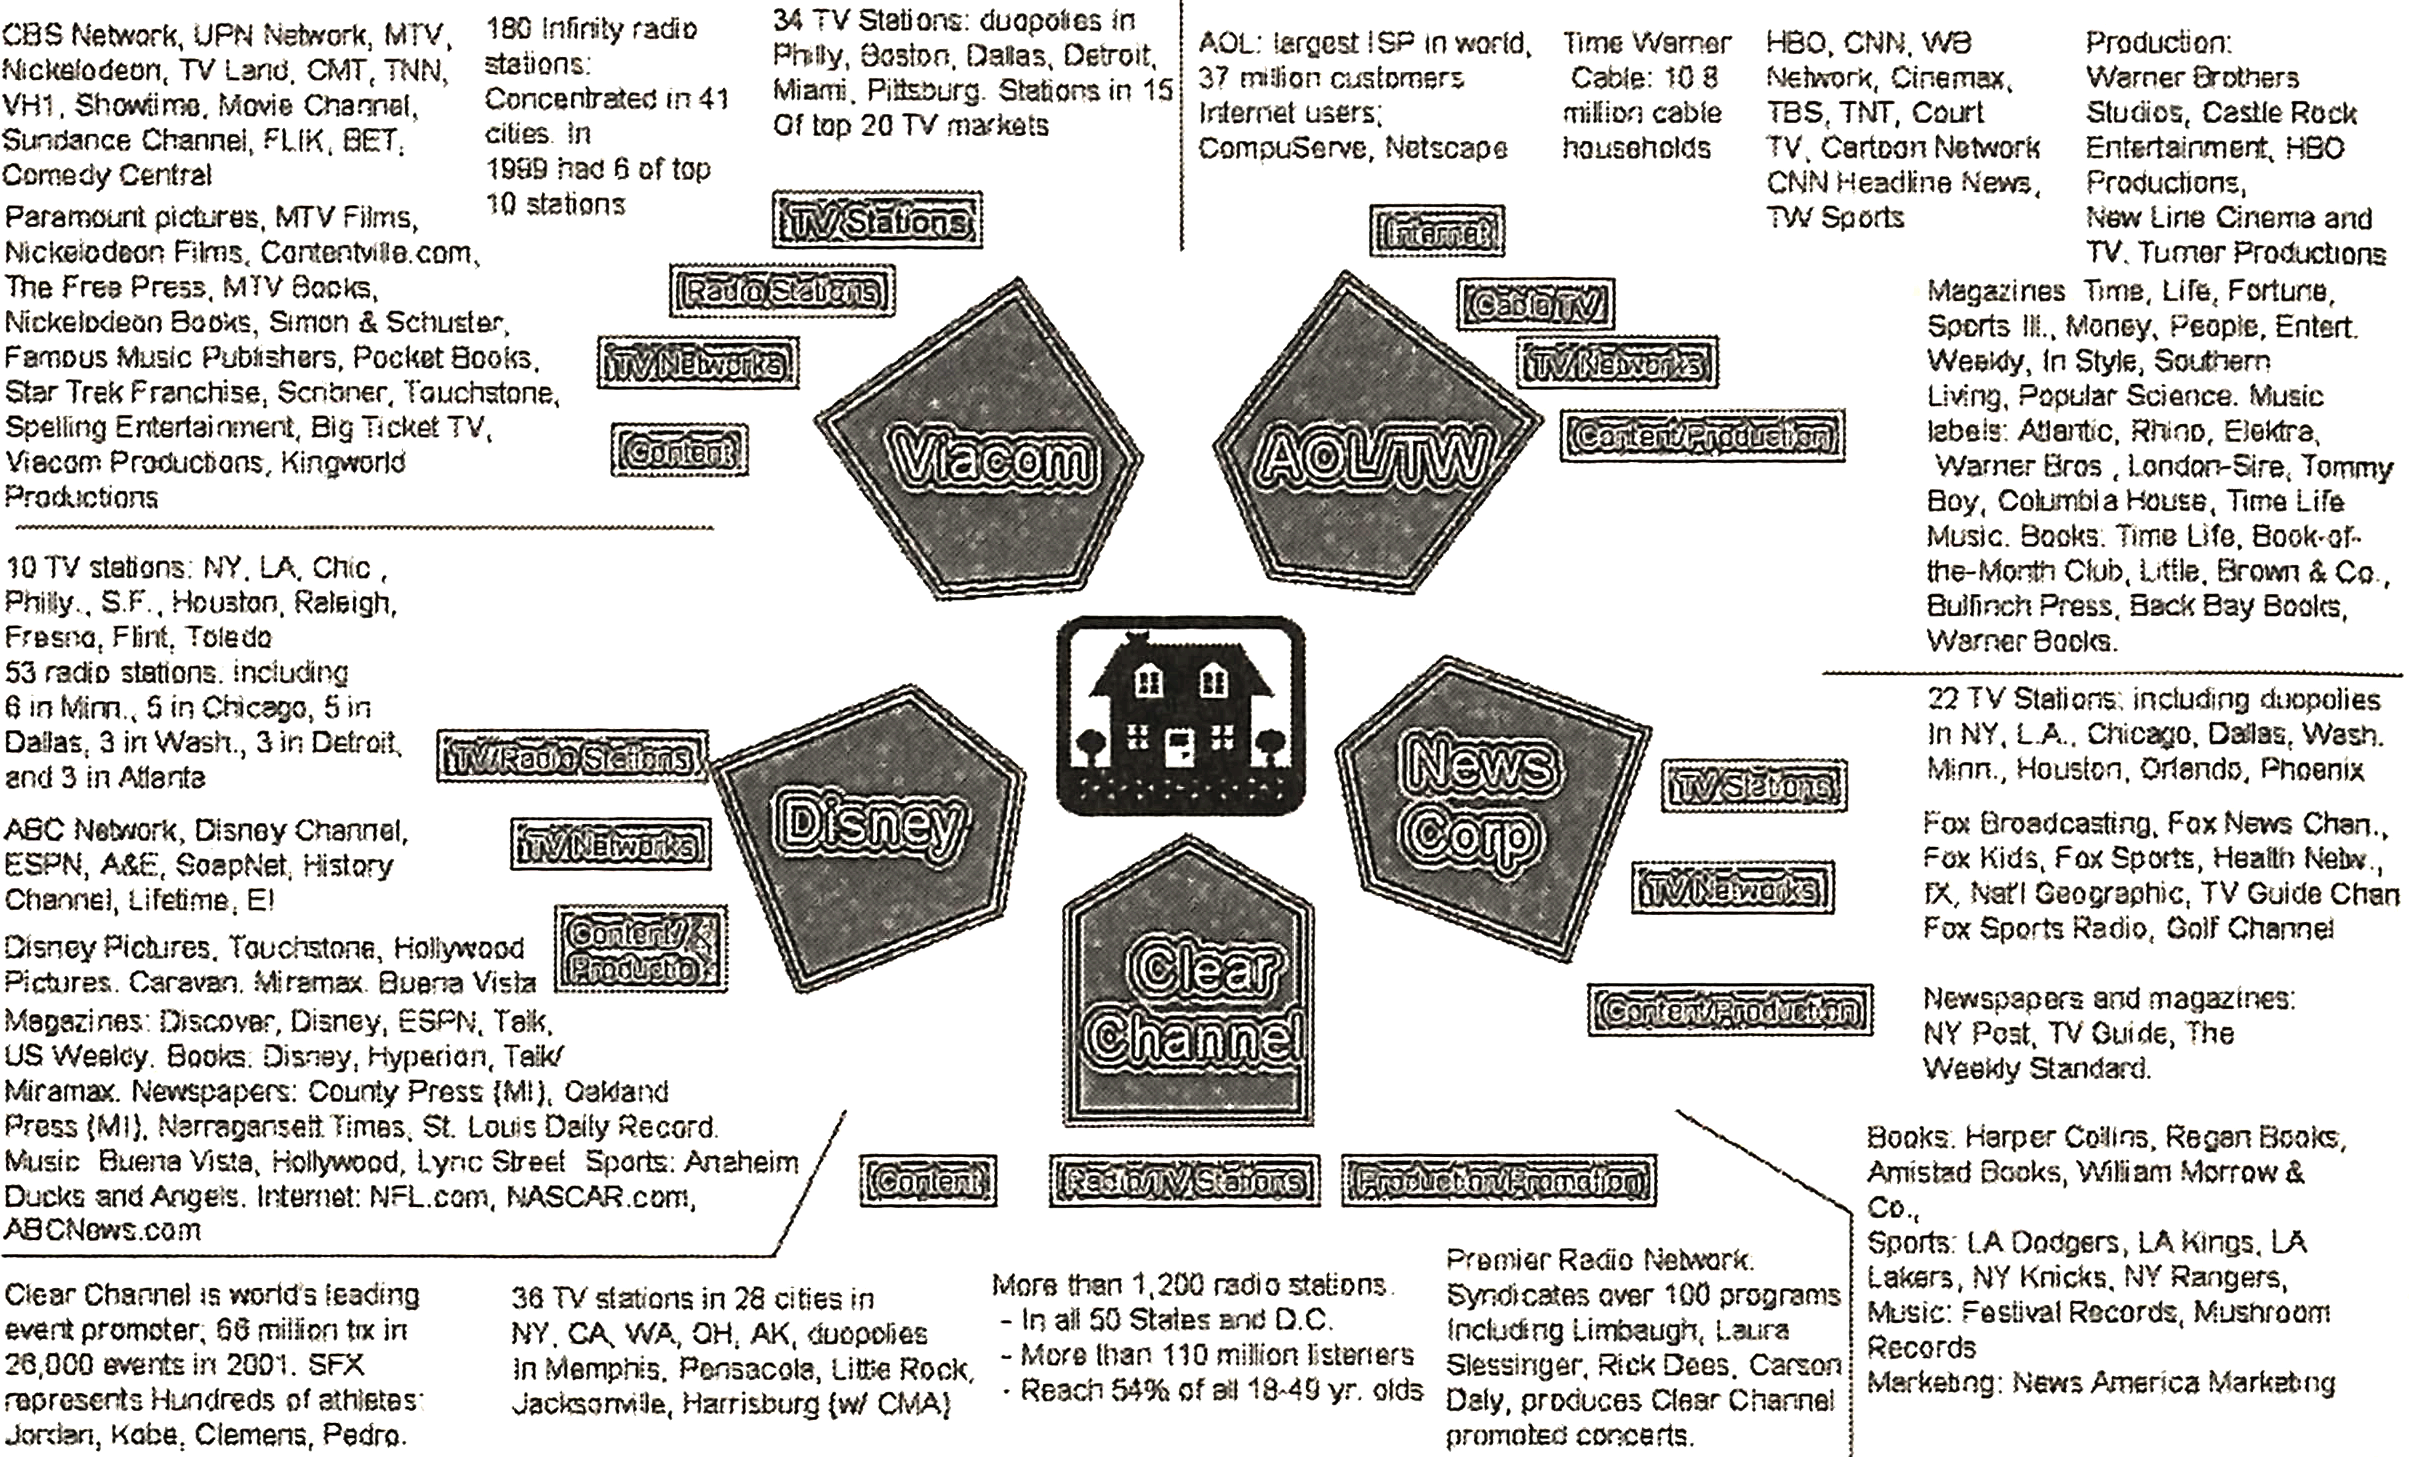
\includegraphics[width=1\linewidth,keepaspectratio=true]{images/pattern-modern-media-ownership.png}}}}{[images/pattern-{}modern-{}media-{}ownership.png not found]}
\end{center}
\addtocounter{figure}{-1}\caption{}
\end{figure}

  Does this concentration matter? Will it affect what is made, or
what is distributed? Or is it merely a more efficient way to produce and
distribute content?


 My view was that concentration wouldn't matter. I thought it was
nothing more than a more efficient financial structure. But now, after
reading and listening to a barrage of creators try to convince me to the
contrary, I am beginning to change my mind.


 Here's a representative story that begins to suggest how this
integration may matter.

\index{Lear, Norman}\index{ABC}\index{All in the Family}

 In 1969, Norman Lear created a pilot for \emph{All in the Family}. He took
the pilot to ABC. The network didn't like it. It was too edgy, they told
Lear. Make it again. Lear made a second pilot, more edgy than the
first. ABC was exasperated. You're missing the point, they told Lear.
We wanted less edgy, not more.


 Rather than comply, Lear simply took the show elsewhere. CBS
was happy to have the series; ABC could not stop Lear from walking.
The copyrights that Lear held assured an independence from network
control.\footnote{
  Leonard Hill, «The Axis of Access,» remarks before Weidenbaum Center
Forum, «Entertainment Economics: The Movie Industry,» St. Louis,
Missouri, 3 April 2003 (transcript of prepared remarks available at
\href{http://free-culture.cc/notes/}{link \#28};
for the Lear story, not included in the prepared remarks, see 
\href{http://free-culture.cc/notes/}{link \#29}).

} 

   The network did not control those copyrights because the law forbade
the networks from controlling the content they syndicated. The law
required a separation between the networks and the content producers;
that separation would guarantee Lear freedom. And as late as 1992,
because of these rules, the vast majority of prime time
television—75 percent of it—was «independent» of the
networks.


 In 1994, the FCC abandoned the rules that required this independence.
After that change, the networks quickly changed the balance.  In 1985,
there were twenty-{}five independent television production studios; in
2002, only five independent television studios remained. «In 1992,
only 15 percent of new series were produced for a network by a company
it controlled. Last year, the percentage of shows produced by
controlled companies more than quintupled to 77 percent.» «In 1992, 16
new series were produced independently of conglomerate control, last
year there was one.»\footnote{
  NewsCorp./DirecTV Merger and Media Consolidation: Hearings on Media
Ownership Before the Senate Commerce Committee, 108th Cong., 1st
sess. (2003) (testimony of Gene Kimmelman on behalf of Consumers Union
and the Consumer Federation of America), available at
\href{http://free-culture.cc/notes/}{link \#30}. Kimmelman
quotes Victoria Riskin, president of Writers Guild of America, West,
in her Remarks at FCC En Banc Hearing, Richmond, Virginia, 27 February
2003.

} In 2002, 75 percent of prime time television was owned by the networks
that ran it. «In the ten-{}year period between 1992 and 2002, the number
of prime time television hours per week produced by network studios
increased over 200\%, whereas the number of prime time television hours
per week produced by independent studios decreased
63\%.»\footnote{
  Ibid.

} 
\index{All in the Family}

 Today, another Norman Lear with another \emph{All in the Family} would
find that he had the choice either to make the show less edgy or to be
fired: The content of any show developed for a network is increasingly
owned by the network.

\index{Diller, Barry}\index{Moyers, Bill}

 While the number of channels has increased dramatically, the ownership
of those channels has narrowed to an ever smaller and smaller few. As
Barry Diller said to Bill Moyers,

\begin{quote}

 Well, if you have companies that produce, that finance, that air on
their channel and then distribute worldwide everything that goes
through their controlled distribution system, then what you get is
fewer and fewer actual voices participating in the process. [We
 u]sed to have dozens and dozens of thriving independent production
companies producing television programs. Now you have less than a
handful.\footnote{
  «Barry Diller Takes on Media Deregulation,» \emph{Now with Bill Moyers}, Bill
Moyers, 25 April 2003, edited transcript available at 
\href{http://free-culture.cc/notes/}{link \#31}.

} 

\end{quote}

 This narrowing has an effect on what is produced. The product of such
large and concentrated networks is increasingly homogenous.
Increasingly safe. Increasingly sterile. The product of news shows
from networks like this is increasingly tailored to the message the
network wants to convey. This is not the communist party, though from
the inside, it must feel a bit like the communist party. No one can
question without risk of consequence—not necessarily banishment
to Siberia, but punishment nonetheless. Independent, critical,
different views are quashed. This is not the environment for a
democracy.

\index{Clark, Kim B.}

 Economics itself offers a parallel that explains why this integration
affects creativity. Clay Christensen has written about the «Innovator's
Dilemma»: the fact that large traditional firms find it rational to ignore
new, breakthrough technologies that compete with their core business.
The same analysis could help explain why large, traditional media
companies would find it rational to ignore new cultural trends.\footnote{
  Clayton M. Christensen, \emph{The Innovator's Dilemma: The
Revolutionary National Bestseller that Changed the Way We Do Business} (Cambridge: Harvard Business School Press, 1997). Christensen
acknowledges that the idea was first suggested by Dean Kim Clark. See
Kim B. Clark, «The Interaction of Design Hierarchies and Market
Concepts in Technological Evolution,» \emph{Research Policy} 14 (1985):
235–51. For a more recent study, see Richard Foster and Sarah
Kaplan, \emph{Creative Destruction: Why Companies That Are Built to Last
Underperform the Market—and How to Successfully Transform Them} (New York: Currency/Doubleday, 2001).  
}  Lumbering giants not only don't, but should not, sprint. Yet if the
field is only open to the giants, there will be far too little
sprinting.
\index{Christensen, Clayton M.} 

 I don't think we know enough about the economics of the media
market to say with certainty what concentration and integration will
do. The efficiencies are important, and the effect on culture is hard to
measure.


 But there is a quintessentially obvious example that does strongly
suggest the concern.


 In addition to the copyright wars, we're in the middle of the drug
wars. Government policy is strongly directed against the drug cartels;
criminal and civil courts are filled with the consequences of this battle.


 Let me hereby disqualify myself from any possible appointment to
any position in government by saying I believe this war is a profound
mistake. I am not pro drugs. Indeed, I come from a family once
  wrecked by drugs—though the drugs that wrecked my family were
all quite legal. I believe this war is a profound mistake because the
collateral damage from it is so great as to make waging the war
insane.  When you add together the burdens on the criminal justice
system, the desperation of generations of kids whose only real
economic opportunities are as drug warriors, the queering of
constitutional protections because of the constant surveillance this
war requires, and, most profoundly, the total destruction of the legal
systems of many South American nations because of the power of the
local drug cartels, I find it impossible to believe that the marginal
benefit in reduced drug consumption by Americans could possibly
outweigh these costs.


 You may not be convinced. That's fine. We live in a democracy, and it
is through votes that we are to choose policy. But to do that, we
depend fundamentally upon the press to help inform Americans about
these issues.

\index{advertising|(}\index{commercials|(}\index{television!advertising on|(}\index{Nick and Norm anti-{}drug campaign}

 Beginning in 1998, the Office of National Drug Control Policy launched
a media campaign as part of the «war on drugs.» The campaign produced
scores of short film clips about issues related to illegal drugs. In
one series (the Nick and Norm series) two men are in a bar, discussing
the idea of legalizing drugs as a way to avoid some of the collateral
damage from the war. One advances an argument in favor of drug
legalization. The other responds in a powerful and effective way
against the argument of the first. In the end, the first guy changes
his mind (hey, it's television). The plug at the end is a damning
attack on the pro-{}legalization campaign.


 Fair enough. It's a good ad. Not terribly misleading. It delivers its
message well. It's a fair and reasonable message.


 But let's say you think it is a wrong message, and you'd like to run a
countercommercial. Say you want to run a series of ads that try to
demonstrate the extraordinary collateral harm that comes from the drug
war. Can you do it?


 Well, obviously, these ads cost lots of money. Assume you raise the
 money. Assume a group of concerned citizens donates all the money in
the world to help you get your message out. Can you be sure your
message will be heard then?

\index{Constitution, U.S.!First Amendment to}\index{First Amendment}\index{Supreme Court, U.S.!on television advertising bans}\index{television!controversy avoided by}

 No. You cannot. Television stations have a general policy of avoiding
«controversial» ads. Ads sponsored by the government are deemed
uncontroversial; ads disagreeing with the government are
controversial.  This selectivity might be thought inconsistent with
the First Amendment, but the Supreme Court has held that stations have
the right to choose what they run. Thus, the major channels of
commercial media will refuse one side of a crucial debate the
opportunity to present its case.  And the courts will defend the
rights of the stations to be this biased.\footnote{
  \index{ABC} \index{Comcast} \index{Marijuana Policy Project} \index{NBC} \index{WJOA} \index{WRC} \index{advertising} The Marijuana Policy Project, in February 2003, sought to place ads
that directly responded to the Nick and Norm series on stations within
the Washington, D.C., area. Comcast rejected the ads as «against
[their] policy.»  The local NBC affiliate, WRC, rejected the ads
without reviewing them. The local ABC affiliate, WJOA, originally
agreed to run the ads and accepted payment to do so, but later decided
not to run the ads and returned the collected fees. Interview with
Neal Levine, 15 October 2003.  These restrictions are, of course, not
limited to drug policy. See, for example, Nat Ives, «On the
Issue of an Iraq War, Advocacy Ads Meet with Rejection from TV
Networks,» \emph{New York Times}, 13 March
2003, C4.  Outside of election-{}related air time there is very little
that the FCC or the courts are willing to do to even the playing
field. For a general overview, see Rhonda Brown, «Ad Hoc Access:
The Regulation of Editorial Advertising on Television and
Radio,» \emph{Yale Law and Policy Review} 6
(1988): 449–79, and for a more recent summary of the stance of
the FCC and the courts, see \emph{Radio-{}Television News Directors
Association} v. \emph{FCC}, 184 F. 3d 872
(D.C. Cir. 1999). Municipal authorities exercise the same authority as
the networks. In a recent example from San Francisco, the San
Francisco transit authority rejected an ad that criticized its Muni
diesel buses. Phillip Matier and Andrew Ross, «Antidiesel Group
Fuming After Muni Rejects Ad,» SFGate.com, 16 June 2003,
available at \href{http://free-culture.cc/notes/}{link
\#32}. The ground was that the criticism was «too
controversial.» 
} 
\index{commercials|)}\index{television!advertising on|)}
 I'd be happy to defend the networks' rights, as well—if we lived
in a media market that was truly diverse. But concentration in the
media throws that condition into doubt. If a handful of companies
control access to the media, and that handful of companies gets to
decide which political positions it will allow to be promoted on its
channels, then in an obvious and important way, concentration
matters. You might like the positions the handful of companies
selects. But you should not like a world in which a mere few get to
decide which issues the rest of us get to know about.

\index{advertising|)}
\section{Together}
\label{together}\hyperlabel{together}%

 There is something innocent and obvious about the claim of the
copyright warriors that the government should «protect my property.» In the abstract, it is obviously true and, ordinarily, totally
harmless. No sane sort who is not an anarchist could disagree.


 But when we see how dramatically this «property» has changed—
when we recognize how it might now interact with both technology and
markets to mean that the effective constraint on the liberty to
cultivate our culture is dramatically different—the claim begins
to seem
  less innocent and obvious. Given (1) the power of technology to
supplement the law's control, and (2) the power of concentrated
markets to weaken the opportunity for dissent, if strictly enforcing
the massively expanded «property» rights granted by copyright
fundamentally changes the freedom within this culture to cultivate and
build upon our past, then we have to ask whether this property should
be redefined.


 Not starkly. Or absolutely. My point is not that we should abolish
copyright or go back to the eighteenth century. That would be a total
mistake, disastrous for the most important creative enterprises within
our culture today.


 But there is a space between zero and one, Internet culture
notwithstanding.  And these massive shifts in the effective power of
copyright regulation, tied to increased concentration of the content
industry and resting in the hands of technology that will increasingly
enable control over the use of culture, should drive us to consider
whether another adjustment is called for. Not an adjustment that
increases copyright's power. Not an adjustment that increases its
term. Rather, an adjustment to restore the balance that has
traditionally defined copyright's regulation—a weakening of that
regulation, to strengthen creativity.


 Copyright law has not been a rock of Gibraltar. It's not a set of
constant commitments that, for some mysterious reason, teenagers and
geeks now flout. Instead, copyright power has grown dramatically in a
short period of time, as the technologies of distribution and creation
have changed and as lobbyists have pushed for more control by
copyright holders. Changes in the past in response to changes in
technology suggest that we may well need similar changes in the
future. And these changes have to be \emph{reductions} in the scope of copyright, in response to the extraordinary increase
in control that technology and the market enable.


 For the single point that is lost in this war on pirates is a point that
we see only after surveying the range of these changes. When you add
 together the effect of changing law, concentrated markets, and
changing technology, together they produce an astonishing conclusion:
\emph{Never in our history have fewer had a legal right to control
more of the development of our culture than now}.


 Not when copyrights were perpetual, for when copyrights were
perpetual, they affected only that precise creative work. Not when
only publishers had the tools to publish, for the market then was much
more diverse. Not when there were only three television networks, for
even then, newspapers, film studios, radio stations, and publishers
were independent of the networks. \emph{Never} has
copyright protected such a wide range of rights, against as broad a
range of actors, for a term that was remotely as long. This form of
regulation—a tiny regulation of a tiny part of the creative
energy of a nation at the founding—is now a massive regulation
of the overall creative process. Law plus technology plus the market
now interact to turn this historically benign regulation into the most
significant regulation of culture that our free society has
known.\footnote{
  \index{Vaidhyanathan, Siva} Siva Vaidhyanathan captures a similar point in his «four surrenders» of
copyright law in the digital age. See Vaidhyanathan, 159–60.

} 

 \textbf{This has been} a long chapter. Its
point can now be briefly stated.


 At the start of this book, I distinguished between commercial and
noncommercial culture. In the course of this chapter, I have
distinguished between copying a work and transforming it. We can now
combine these two distinctions and draw a clear map of the changes
that copyright law has undergone.  In 1790, the law looked like this:



{\centering\savetablecounter \begingroup%
\setlength{\newtblsparewidth}{\linewidth-2\tabcolsep-2\tabcolsep-2\tabcolsep-2\tabcolsep}%
\setlength{\newtblstarfactor}{\newtblsparewidth / \real{3}}%

\begin{longtable}{lll}\hline
\multicolumn{1}{|m{\newtblstarfactor}|}{\raggedright\bfseries%
%
%
}&\multicolumn{1}{m{\newtblstarfactor}|}{\raggedright\bfseries%
%
PUBLISH%
}&\multicolumn{1}{m{\newtblstarfactor}|}{\raggedright\bfseries%
%
TRANSFORM%
}\tabularnewline
\cline{1-1}\cline{2-2}\cline{3-3}\endhead
\multicolumn{1}{|m{\newtblstarfactor}|}{\raggedright%
Commercial%
}&\multicolumn{1}{m{\newtblstarfactor}|}{\raggedright%
©%
}&\multicolumn{1}{m{\newtblstarfactor}|}{\raggedright%
Free%
}\tabularnewline
\cline{1-1}\cline{2-2}\cline{3-3}\multicolumn{1}{|m{\newtblstarfactor}|}{\raggedright%
Noncommercial%
}&\multicolumn{1}{m{\newtblstarfactor}|}{\raggedright%
Free%
}&\multicolumn{1}{m{\newtblstarfactor}|}{\raggedright%
Free%
}\tabularnewline
\hline
\end{longtable}\endgroup%
\restoretablecounter%
}

 The act of publishing a map, chart, and book was regulated by
copyright law. Nothing else was. Transformations were free. And as
copyright attached only with registration, and only those who intended
  to benefit commercially would register, copying through publishing of
noncommercial work was also free.


 By the end of the nineteenth century, the law had changed to this:



{\centering\savetablecounter \begingroup%
\setlength{\newtblsparewidth}{\linewidth-2\tabcolsep-2\tabcolsep-2\tabcolsep-2\tabcolsep}%
\setlength{\newtblstarfactor}{\newtblsparewidth / \real{3}}%

\begin{longtable}{lll}\hline
\multicolumn{1}{|m{\newtblstarfactor}|}{\raggedright\bfseries%
%
%
}&\multicolumn{1}{m{\newtblstarfactor}|}{\raggedright\bfseries%
%
PUBLISH%
}&\multicolumn{1}{m{\newtblstarfactor}|}{\raggedright\bfseries%
%
TRANSFORM%
}\tabularnewline
\cline{1-1}\cline{2-2}\cline{3-3}\endhead
\multicolumn{1}{|m{\newtblstarfactor}|}{\raggedright%
Commercial%
}&\multicolumn{1}{m{\newtblstarfactor}|}{\raggedright%
©%
}&\multicolumn{1}{m{\newtblstarfactor}|}{\raggedright%
©%
}\tabularnewline
\cline{1-1}\cline{2-2}\cline{3-3}\multicolumn{1}{|m{\newtblstarfactor}|}{\raggedright%
Noncommercial%
}&\multicolumn{1}{m{\newtblstarfactor}|}{\raggedright%
Free%
}&\multicolumn{1}{m{\newtblstarfactor}|}{\raggedright%
Free%
}\tabularnewline
\hline
\end{longtable}\endgroup%
\restoretablecounter%
}

 Derivative works were now regulated by copyright law—if
published, which again, given the economics of publishing at the time,
means if offered commercially. But noncommercial publishing and
transformation were still essentially free.


 In 1909 the law changed to regulate copies, not publishing, and after
this change, the scope of the law was tied to technology. As the
technology of copying became more prevalent, the reach of the law
expanded.  Thus by 1975, as photocopying machines became more common,
we could say the law began to look like this:



{\centering\savetablecounter \begingroup%
\setlength{\newtblsparewidth}{\linewidth-2\tabcolsep-2\tabcolsep-2\tabcolsep-2\tabcolsep}%
\setlength{\newtblstarfactor}{\newtblsparewidth / \real{3}}%

\begin{longtable}{lll}\hline
\multicolumn{1}{|m{\newtblstarfactor}|}{\raggedright\bfseries%
%
%
}&\multicolumn{1}{m{\newtblstarfactor}|}{\raggedright\bfseries%
%
COPY%
}&\multicolumn{1}{m{\newtblstarfactor}|}{\raggedright\bfseries%
%
TRANSFORM%
}\tabularnewline
\cline{1-1}\cline{2-2}\cline{3-3}\endhead
\multicolumn{1}{|m{\newtblstarfactor}|}{\raggedright%
Commercial%
}&\multicolumn{1}{m{\newtblstarfactor}|}{\raggedright%
©%
}&\multicolumn{1}{m{\newtblstarfactor}|}{\raggedright%
©%
}\tabularnewline
\cline{1-1}\cline{2-2}\cline{3-3}\multicolumn{1}{|m{\newtblstarfactor}|}{\raggedright%
Noncommercial%
}&\multicolumn{1}{m{\newtblstarfactor}|}{\raggedright%
© / Free%
}&\multicolumn{1}{m{\newtblstarfactor}|}{\raggedright%
Free%
}\tabularnewline
\hline
\end{longtable}\endgroup%
\restoretablecounter%
}

 The law was interpreted to reach noncommercial copying through, say,
copy machines, but still much of copying outside of the commercial
market remained free. But the consequence of the emergence of digital
technologies, especially in the context of a digital network, means
that the law now looks like this:



{\centering\savetablecounter \begingroup%
\setlength{\newtblsparewidth}{\linewidth-2\tabcolsep-2\tabcolsep-2\tabcolsep-2\tabcolsep}%
\setlength{\newtblstarfactor}{\newtblsparewidth / \real{3}}%

\begin{longtable}{lll}\hline
\multicolumn{1}{|m{\newtblstarfactor}|}{\raggedright\bfseries%
%
%
}&\multicolumn{1}{m{\newtblstarfactor}|}{\raggedright\bfseries%
%
COPY%
}&\multicolumn{1}{m{\newtblstarfactor}|}{\raggedright\bfseries%
%
TRANSFORM%
}\tabularnewline
\cline{1-1}\cline{2-2}\cline{3-3}\endhead
\multicolumn{1}{|m{\newtblstarfactor}|}{\raggedright%
Commercial%
}&\multicolumn{1}{m{\newtblstarfactor}|}{\raggedright%
©%
}&\multicolumn{1}{m{\newtblstarfactor}|}{\raggedright%
©%
}\tabularnewline
\cline{1-1}\cline{2-2}\cline{3-3}\multicolumn{1}{|m{\newtblstarfactor}|}{\raggedright%
Noncommercial%
}&\multicolumn{1}{m{\newtblstarfactor}|}{\raggedright%
©%
}&\multicolumn{1}{m{\newtblstarfactor}|}{\raggedright%
©%
}\tabularnewline
\hline
\end{longtable}\endgroup%
\restoretablecounter%
}

 Every realm is governed by copyright law, whereas before most
creativity was not. The law now regulates the full range of
creativity—
 commercial or not, transformative or not—with the same rules
designed to regulate commercial publishers.


 Obviously, copyright law is not the enemy. The enemy is regulation
that does no good. So the question that we should be asking just now
is whether extending the regulations of copyright law into each of
these domains actually does any good.


 I have no doubt that it does good in regulating commercial copying.
But I also have no doubt that it does more harm than good when
regulating (as it regulates just now) noncommercial copying and,
especially, noncommercial transformation. And increasingly, for the
reasons sketched especially in chapters
\ref{recorders} [\pageref{recorders}] and
\ref{transformers} [\pageref{transformers}], one
might well wonder whether it does more harm than good for commercial
transformation.  More commercial transformative work would be created
if derivative rights were more sharply restricted.


 The issue is therefore not simply whether copyright is property. Of
course copyright is a kind of «property,» and of course, as with any
property, the state ought to protect it. But first impressions
notwithstanding, historically, this property right (as with all
property rights\footnote{
  \index{legal realist movement} It was the single most important contribution of the legal realist
movement to demonstrate that all property rights are always crafted to
balance public and private interests. See Thomas C. Grey, «The
Disintegration of Property,» in \emph{Nomos XXII: Property}, J. Roland
Pennock and John W.  Chapman, eds. (New York: New York University
Press, 1980).

})
has been crafted to balance the important need to give authors and
artists incentives with the equally important need to assure access to
creative work. This balance has always been struck in light of new
technologies.  And for almost half of our tradition, the «copyright» did not control \emph{at all} the freedom of others to
build upon or transform a creative work. American culture was born
free, and for almost 180 years our country consistently protected a
vibrant and rich free culture.

\index{archives, digital}

 We achieved that free culture because our law respected important
limits on the scope of the interests protected by «property.» The very
birth of «copyright» as a statutory right recognized those limits, by
granting copyright owners protection for a limited time only (the
story of chapter \ref{founders} [\pageref{founders}]). The tradition of «fair use» is
animated by a similar concern that is increasingly under strain as the
costs of exercising any fair use right become unavoidably high (the
story of chapter \ref{recorders} [\pageref{recorders}]). Adding
 statutory rights where markets might stifle innovation is another
familiar limit on the property right that copyright is (chapter \ref{transformers} [\pageref{transformers}]). And
granting archives and libraries a broad freedom to collect, claims of
property notwithstanding, is a crucial part of guaranteeing the soul
of a culture (chapter \ref{collectors} [\pageref{collectors}]). Free cultures, like free markets, are built
with property. But the nature of the property that builds a free
culture is very different from the extremist vision that dominates the
debate today.


 Free culture is increasingly the casualty in this war on piracy. In
response to a real, if not yet quantified, threat that the
technologies of the Internet present to twentieth-{}century business
models for producing and distributing culture, the law and technology
are being transformed in a way that will undermine our tradition of
free culture. The property right that is copyright is no longer the
balanced right that it was, or was intended to be. The property right
that is copyright has become unbalanced, tilted toward an extreme. The
opportunity to create and transform becomes weakened in a world in
which creation requires permission and creativity must check with a
lawyer.

%
% PART
%

\part{Puzzles}
\label{c-puzzles}\hyperlabel{c-puzzles}%

% ------- 
% Chapter 
% ------- 
\setcounter{chapter}{10}

\chapter{Chapter Eleven: Chimera}
\label{chimera}\hyperlabel{chimera}%
\index{chimeras|(}\index{Wells, H. G.|(}\index{Country of the Blind, The (Wells)|(}

 \textbf{In a well-{}known} short story by
H. G. Wells, a mountain climber named Nunez trips (literally, down an
ice slope) into an unknown and isolated valley in the Peruvian
Andes.\footnote{
  H. G. Wells, «The Country of the Blind» (1904, 1911). See H. G. Wells,
\emph{The Country of the Blind and Other Stories}, Michael Sherborne, ed. (New
York: Oxford University Press, 1996).

} The valley is extraordinarily beautiful, with «sweet water, pasture,
an even climate, slopes of rich brown soil with tangles of a shrub
that bore an excellent fruit.» But the villagers are all blind. Nunez
takes this as an opportunity. «In the Country of the Blind,» he tells
himself, «the One-{}Eyed Man is King.»  So he resolves to live with the
villagers to explore life as a king.


 Things don't go quite as he planned. He tries to explain the idea of
sight to the villagers. They don't understand. He tells them they are
«blind.» They don't have the word \emph{blind}. They think he's just thick.
Indeed, as they increasingly notice the things he can't do (hear the
sound of grass being stepped on, for example), they increasingly try
to control him. He, in turn, becomes increasingly frustrated. «\`{}You
don't understand,' he cried, in a voice that was meant to be great and
resolute, and which broke. \`{}You are blind and I can see. Leave me
alone!'» 

  The villagers don't leave him alone. Nor do they see (so to speak) the
virtue of his special power. Not even the ultimate target of his
affection, a young woman who to him seems «the most beautiful thing in
the whole of creation,» understands the beauty of sight. Nunez's
description of what he sees «seemed to her the most poetical of
fancies, and she listened to his description of the stars and the
mountains and her own sweet white-{}lit beauty as though it was a guilty
indulgence.» «She did not believe,» Wells tells us, and «she could
only half understand, but she was mysteriously delighted.» 

 When Nunez announces his desire to marry his «mysteriously delighted» love, the father and the village object. «You see, my dear,» her
father instructs, «he's an idiot. He has delusions. He can't do
anything right.» They take Nunez to the village doctor.


 After a careful examination, the doctor gives his opinion. «His brain
is affected,» he reports.


 «What affects it?» the father asks.  «Those queer things that are
called the eyes … are diseased … in such a way as to affect
his brain.» 

 The doctor continues: «I think I may say with reasonable certainty
that in order to cure him completely, all that we need to do is a
simple and easy surgical operation—namely, to remove these
irritant bodies [the eyes].» 

 «Thank Heaven for science!» says the father to the doctor. They inform
Nunez of this condition necessary for him to be allowed his bride.
(You'll have to read the original to learn what happens in the end. I
believe in free culture, but never in giving away the end of a story.)


 \textbf{It sometimes} happens that the eggs
of twins fuse in the mother's womb. That fusion produces a
«chimera.» A chimera is a single creature with two sets
of DNA. The DNA in the blood, for example, might be different from the
DNA of the skin. This possibility is an underused
  plot for murder mysteries. «But the DNA shows with 100 percent
certainty that she was not the person whose blood was at the
scene. …» 
\index{Country of the Blind, The (Wells)|)}
\index{Wells, H. G.|)}
 Before I had read about chimeras, I would have said they were
impossible.  A single person can't have two sets of DNA. The very idea
of DNA is that it is the code of an individual. Yet in fact, not only
can two individuals have the same set of DNA (identical twins), but
one person can have two different sets of DNA (a chimera). Our
understanding of a «person» should reflect this reality.


 The more I work to understand the current struggle over copyright and
culture, which I've sometimes called unfairly, and sometimes not
unfairly enough, «the copyright wars,» the more I think we're dealing
with a chimera. For example, in the battle over the question «What is
p2p file sharing?» both sides have it right, and both sides have it
wrong.  One side says, «File sharing is just like two kids taping each
others' records—the sort of thing we've been doing for the last
thirty years without any question at all.» That's true, at least in
part. When I tell my best friend to try out a new CD that I've bought,
but rather than just send the CD, I point him to my p2p server, that
is, in all relevant respects, just like what every executive in every
recording company no doubt did as a kid: sharing music.


 But the description is also false in part. For when my p2p server is
on a p2p network through which anyone can get access to my music, then
sure, my friends can get access, but it stretches the meaning of
«friends» beyond recognition to say «my ten thousand best friends» can
get access. Whether or not sharing my music with my best friend is
what «we have always been allowed to do,» we have not always been
allowed to share music with «our ten thousand best friends.» 

 Likewise, when the other side says, «File sharing is just like walking
into a Tower Records and taking a CD off the shelf and walking out
with it,» that's true, at least in part. If, after Lyle Lovett
(finally) releases a new album, rather than buying it, I go to Kazaa
and find a free copy to take, that is very much like stealing a copy
from Tower.
\index{Lovett, Lyle} 

   But it is not quite stealing from Tower. After all, when I take a CD
from Tower Records, Tower has one less CD to sell. And when I take a
CD from Tower Records, I get a bit of plastic and a cover, and
something to show on my shelves. (And, while we're at it, we could
also note that when I take a CD from Tower Records, the maximum fine
that might be imposed on me, under California law, at least, is
\$1,000.  According to the RIAA, by contrast, if I download a ten-{}song
CD, I'm liable for \$1,500,000 in damages.)


 The point is not that it is as neither side describes. The point is
that it is both—both as the RIAA describes it and as Kazaa
describes it. It is a chimera. And rather than simply denying what the
other side asserts, we need to begin to think about how we should
respond to this chimera. What rules should govern it?


 We could respond by simply pretending that it is not a chimera. We
could, with the RIAA, decide that every act of file sharing should be
a felony. We could prosecute families for millions of dollars in
damages just because file sharing occurred on a family computer. And
we can get universities to monitor all computer traffic to make sure
that no computer is used to commit this crime. These responses might
be extreme, but each of them has either been proposed or actually
implemented.\footnote{
  \index{ISPs (Internet service providers), user identities revealed by} For an excellent summary, see the report prepared by GartnerG2 and the
Berkman Center for Internet and Society at Harvard Law School,
«Copyright and Digital Media in a Post-{}Napster World,» 27 June 2003,
available at
\href{http://free-culture.cc/notes/}{link
\#33}. Reps. John Conyers Jr. (D-{}Mich.) and Howard L. Berman
(D-{}Calif.) have introduced a bill that would treat unauthorized
on-{}line copying as a felony offense with punishments ranging as high
as five years imprisonment; see Jon Healey, «House Bill Aims to Up
Stakes on Piracy,» \emph{Los Angeles Times}, 17 July 2003, available at
\href{http://free-culture.cc/notes/}{link \#34}. Civil
penalties are currently set at \$150,000 per copied song. For a recent
(and unsuccessful) legal challenge to the RIAA's demand that an ISP
reveal the identity of a user accused of sharing more than 600 songs
through a family computer, see \emph{RIAA} v. \emph{Verizon Internet Services (In
re. Verizon Internet Services)}, 240 F.  Supp. 2d 24
(D.D.C. 2003). Such a user could face liability ranging as high as \$90
million. Such astronomical figures furnish the RIAA with a powerful
arsenal in its prosecution of file sharers. Settlements ranging from
\$12,000 to \$17,500 for four students accused of heavy file sharing on
university networks must have seemed a mere pittance next to the \$98
billion the RIAA could seek should the matter proceed to court. See
Elizabeth Young, «Downloading Could Lead to Fines,» redandblack.com,
August 2003, available at
\href{http://free-culture.cc/notes/}{link \#35}. For an
example of the RIAA's targeting of student file sharing, and of the
subpoenas issued to universities to reveal student file-{}sharer
identities, see James Collins, «RIAA Steps Up Bid to Force BC, MIT to
Name Students,» \emph{Boston Globe}, 8 August 2003, D3, available at
\href{http://free-culture.cc/notes/}{link \#36}.
\index{Conyers, John, Jr.} \index{Berman, Howard L.} 
}  
\index{chimeras|)}
 Alternatively, we could respond to file sharing the way many kids act
as though we've responded. We could totally legalize it. Let there be
no copyright liability, either civil or criminal, for making
copyrighted content available on the Net. Make file sharing like
gossip: regulated, if at all, by social norms but not by law.


 Either response is possible. I think either would be a mistake.
Rather than embrace one of these two extremes, we should embrace
something that recognizes the truth in both. And while I end this book
with a sketch of a system that does just that, my aim in the next
chapter is to show just how awful it would be for us to adopt the
zero-{}tolerance extreme. I believe \emph{either} extreme
would be worse than a reasonable alternative.  But I believe the
zero-{}tolerance solution would be the worse of the two extremes.


   Yet zero tolerance is increasingly our government's policy. In the
middle of the chaos that the Internet has created, an extraordinary
land grab is occurring. The law and technology are being shifted to
give content holders a kind of control over our culture that they have
never had before. And in this extremism, many an opportunity for new
innovation and new creativity will be lost.


 I'm not talking about the opportunities for kids to «steal» music. My
focus instead is the commercial and cultural innovation that this war
will also kill. We have never seen the power to innovate spread so
broadly among our citizens, and we have just begun to see the
innovation that this power will unleash. Yet the Internet has already
seen the passing of one cycle of innovation around technologies to
distribute content. The law is responsible for this passing. As the
vice president for global public policy at one of these new
innovators, eMusic.com, put it when criticizing the DMCA's added
protection for copyrighted material,

\begin{quote}

 eMusic opposes music piracy. We are a distributor of copyrighted
material, and we want to protect those rights.


 But building a technology fortress that locks in the clout of the
major labels is by no means the only way to protect copyright
interests, nor is it necessarily the best. It is simply too early to
answer that question. Market forces operating naturally may very well
produce a totally different industry model.


 This is a critical point. The choices that industry sectors make
with respect to these systems will in many ways directly shape the
market for digital media and the manner in which digital media
are distributed. This in turn will directly influence the options
that are available to consumers, both in terms of the ease with
which they will be able to access digital media and the equipment
that they will require to do so. Poor choices made this early in the
game will retard the growth of this market, hurting everyone's
interests.\footnote{
  WIPO and the DMCA One Year Later: Assessing Consumer Access to Digital
Entertainment on the Internet and Other Media: Hearing Before the
Subcommittee on Telecommunications, Trade, and Consumer Protection,
House Committee on Commerce, 106th Cong. 29 (1999) (statement of Peter
Harter, vice president, Global Public Policy and Standards,
EMusic.com), available in LEXIS, Federal Document Clearing House
Congressional Testimony File.  
} 

\end{quote}

 In April 2001, eMusic.com was purchased by Vivendi Universal,
one of «the major labels.» Its position on these matters has now
changed.
\index{Vivendi Universal} 

 Reversing our tradition of tolerance now will not merely quash
piracy. It will sacrifice values that are important to this culture,
and will kill opportunities that could be extraordinarily valuable.


% ------- 
% Chapter 
% ------- 
\setcounter{chapter}{11}

\chapter{Chapter Twelve: Harms}
\label{harms}\hyperlabel{harms}%

 \textbf{To fight} «piracy,» to
protect «property,» the content industry has launched a
war. Lobbying and lots of campaign contributions have now brought the
government into this war. As with any war, this one will have both
direct and collateral damage. As with any war of prohibition, these
damages will be suffered most by our own people.


 My aim so far has been to describe the consequences of this war, in
particular, the consequences for «free culture.» But my aim now is to
extend this description of consequences into an argument. Is this war
justified?


 In my view, it is not. There is no good reason why this time, for the
first time, the law should defend the old against the new, just when the
power of the property called «intellectual property» is at its greatest in
our history.

\index{Causby, Thomas Lee}\index{Causby, Tinie}

 Yet «common sense» does not see it this way. Common sense is still on
the side of the Causbys and the content industry. The extreme claims
of control in the name of property still resonate; the uncritical
rejection of «piracy» still has play.

\index{Armstrong, Edwin Howard}

  There will be many consequences of continuing this war. I want to
describe just three. All three might be said to be unintended. I am quite
confident the third is unintended. I'm less sure about the first two. The
first two protect modern RCAs, but there is no Howard Armstrong in
the wings to fight today's monopolists of culture.


\section{Constraining Creators}
\label{constrain}\hyperlabel{constrain}%

 In the next ten years we will see an explosion of digital
technologies.  These technologies will enable almost anyone to capture
and share content. Capturing and sharing content, of course, is what
humans have done since the dawn of man. It is how we learn and
communicate. But capturing and sharing through digital technology is
different. The fidelity and power are different. You could send an
e-{}mail telling someone about a joke you saw on Comedy Central, or you
could send the clip. You could write an essay about the
inconsistencies in the arguments of the politician you most love to
hate, or you could make a short film that puts statement against
statement. You could write a poem to express your love, or you could
weave together a string—a mash-{}up— of songs from your
favorite artists in a collage and make it available on the Net.


 This digital «capturing and sharing» is in part an extension of the
capturing and sharing that has always been integral to our culture,
and in part it is something new. It is continuous with the Kodak, but
it explodes the boundaries of Kodak-{}like technologies. The technology
of digital «capturing and sharing» promises a world of extraordinarily
diverse creativity that can be easily and broadly shared. And as that
creativity is applied to democracy, it will enable a broad range of
citizens to use technology to express and criticize and contribute to
the culture all around.


 Technology has thus given us an opportunity to do something with
culture that has only ever been possible for individuals in small groups,
   isolated from others. Think about an old man telling a story to a
collection of neighbors in a small town. Now imagine that same
storytelling extended across the globe.


 Yet all this is possible only if the activity is presumptively legal. In
the current regime of legal regulation, it is not. Forget file sharing for
a moment. Think about your favorite amazing sites on the Net. Web
sites that offer plot summaries from forgotten television shows; sites
that catalog cartoons from the 1960s; sites that mix images and sound
to criticize politicians or businesses; sites that gather newspaper articles
on remote topics of science or culture. There is a vast amount of creative
work spread across the Internet. But as the law is currently crafted, this
work is presumptively illegal.

\index{WorldCom}\index{copyright infringement lawsuits!exaggerated claims of}\index{copyright infringement lawsuits!in recording industry}\index{doctors malpractice claims against}\index{Jordan, Jesse}

 That presumption will increasingly chill creativity, as the
examples of extreme penalties for vague infringements continue to
proliferate. It is impossible to get a clear sense of what's allowed
and what's not, and at the same time, the penalties for crossing the
line are astonishingly harsh.  The four students who were threatened
by the RIAA (Jesse Jordan of chapter \ref{catalogs} [\pageref{catalogs}] was just one) were threatened with a
\$98 billion lawsuit for building search engines that permitted songs
to be copied. Yet World-{}Com—which defrauded investors of \$11
billion, resulting in a loss to investors in market capitalization of
over \$200 billion—received a fine of a mere \$750
million.\footnote{
  See Lynne W. Jeter, \emph{Disconnected: Deceit and Betrayal at WorldCom} (Hoboken, N.J.: John Wiley \& Sons, 2003), 176, 204; for details of
the settlement, see MCI press release, «MCI Wins U.S. District Court
Approval for SEC Settlement» (7 July 2003), available at
\href{http://free-culture.cc/notes/}{link \#37}.
\index{WorldCom} 
} And under legislation being pushed in Congress right now, a doctor who
negligently removes the wrong leg in an operation would be liable for
no more than \$250,000 in damages for pain and
suffering.\footnote{
  The bill, modeled after California's tort reform model, was passed in the
House of Representatives but defeated in a Senate vote in July 2003. For
an overview, see Tanya Albert, «Measure Stalls in Senate: \`{}We'll Be Back,'
Say Tort Reformers,» amednews.com, 28 July 2003, available at 
\href{http://free-culture.cc/notes/}{link \#38},
and «Senate Turns Back Malpractice Caps,» CBSNews.com, 9 July 2003,
available at 
\href{http://free-culture.cc/notes/}{link \#39}. President Bush has continued to urge tort reform in
recent months.
\index{Bush, George W.} 
} Can common sense recognize the absurdity in a world where
the maximum fine for downloading two songs off the Internet is more
than the fine for a doctor's negligently butchering a patient?

\index{art, underground}

 The consequence of this legal uncertainty, tied to these extremely
high penalties, is that an extraordinary amount of creativity will
either never be exercised, or never be exercised in the open. We drive
this creative process underground by branding the modern-{}day Walt
Disneys «pirates.» We make it impossible for businesses to rely upon a
public domain, because the boundaries of the public domain are
designed to
  be unclear. It never pays to do anything except pay for the right
to create, and hence only those who can pay are allowed to create. As
was the case in the Soviet Union, though for very different reasons,
we will begin to see a world of underground art—not because the
message is necessarily political, or because the subject is
controversial, but because the very act of creating the art is legally
fraught. Already, exhibits of «illegal art» tour the United
States.\footnote{
   See Danit Lidor, «Artists Just Wanna Be Free,» \emph{Wired}, 7 July
2003, available at
\href{http://free-culture.cc/notes/}{link \#40}. For an overview of the exhibition, see 
\href{http://free-culture.cc/notes/}{link \#41}.

}  In what does their «illegality» consist?
In the act of mixing the culture around us with an expression that is
critical or reflective.

\index{ISPs (Internet service providers), user identities revealed by}

 Part of the reason for this fear of illegality has to do with the
changing law. I described that change in detail in chapter
\ref{property-i} [\pageref{property-i}]. But an
even bigger part has to do with the increasing ease with which
infractions can be tracked. As users of file-{}sharing systems
discovered in 2002, it is a trivial matter for copyright owners to get
courts to order Internet service providers to reveal who has what
content. It is as if your cassette tape player transmitted a list of
the songs that you played in the privacy of your own home that anyone
could tune into for whatever reason they chose.

\index{images, ownership of}

 Never in our history has a painter had to worry about whether
his painting infringed on someone else's work; but the modern-{}day
painter, using the tools of Photoshop, sharing content on the Web,
must worry all the time. Images are all around, but the only safe images
to use in the act of creation are those purchased from Corbis or another
image farm. And in purchasing, censoring happens. There is a free
market in pencils; we needn't worry about its effect on creativity. But
there is a highly regulated, monopolized market in cultural icons; the
right to cultivate and transform them is not similarly free.


 Lawyers rarely see this because lawyers are rarely empirical. As I
described in chapter
\ref{recorders} [\pageref{recorders}], in
response to the story about documentary filmmaker Jon Else, I have
been lectured again and again by lawyers who insist Else's use was
fair use, and hence I am wrong to say that the law regulates such a
use.


   But fair use in America simply means the right to hire a lawyer to
defend your right to create. And as lawyers love to forget, our system
for defending rights such as fair use is astonishingly bad—in
practically every context, but especially here. It costs too much, it
delivers too slowly, and what it delivers often has little connection
to the justice underlying the claim. The legal system may be tolerable
for the very rich.  For everyone else, it is an embarrassment to a
tradition that prides itself on the rule of law.


 Judges and lawyers can tell themselves that fair use provides adequate
«breathing room» between regulation by the law and the access the law
should allow. But it is a measure of how out of touch our legal system
has become that anyone actually believes this. The rules that
publishers impose upon writers, the rules that film distributors
impose upon filmmakers, the rules that newspapers impose upon
journalists— these are the real laws governing creativity. And
these rules have little relationship to the «law» with which judges
comfort themselves.


 For in a world that threatens \$150,000 for a single willful
infringement of a copyright, and which demands tens of thousands of
dollars to even defend against a copyright infringement claim, and
which would never return to the wrongfully accused defendant anything
of the costs she suffered to defend her right to speak—in that
world, the astonishingly broad regulations that pass under the name
«copyright» silence speech and creativity. And in that world, it takes
a studied blindness for people to continue to believe they live in a
culture that is free.


 As Jed Horovitz, the businessman behind Video Pipeline, said to me,

\begin{quote}

 We're losing [creative] opportunities right and left. Creative people
are being forced not to express themselves. Thoughts are not being
expressed. And while a lot of stuff may [still] be created, it still
won't get distributed. Even if the stuff gets made … you're not
going to get it distributed in the mainstream media unless
 you've got a little note from a lawyer saying, «This has been
cleared.» You're not even going to get it on PBS without that kind of
permission. That's the point at which they control it.


\end{quote}

\section{Constraining Innovators}
\label{innovators}\hyperlabel{innovators}%
\index{copyright law!innovation hampered by|(}\index{innovation!industry establishment opposed to|(}\index{regulation!as establishment protectionism|(}

 The story of the last section was a crunchy-{}lefty
story—creativity quashed, artists who can't speak, yada yada
yada. Maybe that doesn't get you going. Maybe you think there's enough
weird art out there, and enough expression that is critical of what
seems to be just about everything.  And if you think that, you might
think there's little in this story to worry you.

\index{market constraints|(}

 But there's an aspect of this story that is not lefty in any sense.
Indeed, it is an aspect that could be written by the most extreme
promarket ideologue. And if you're one of these sorts (and a special
one at that, \pageref{innovators} pages into a book like this), then you
can see this other aspect by substituting «free market» every place I've spoken of «free culture.» The point is
the same, even if the interests affecting culture are more
fundamental.


 The charge I've been making about the regulation of culture is the
same charge free marketers make about regulating markets. Everyone, of
course, concedes that some regulation of markets is necessary—at
a minimum, we need rules of property and contract, and courts to
enforce both. Likewise, in this culture debate, everyone concedes that
at least some framework of copyright is also required. But both
perspectives vehemently insist that just because some regulation is
good, it doesn't follow that more regulation is better. And both
perspectives are constantly attuned to the ways in which regulation
simply enables the powerful industries of today to protect themselves
against the competitors of tomorrow.

\index{market constraints|)}
\index{Barry, Hank}\index{venture capitalists}

 This is the single most dramatic effect of the shift in regulatory
 strategy that I described in chapter \ref{property-i} [\pageref{property-i}]. The consequence of this massive
threat of liability tied to the murky boundaries of copyright law is
that innovators who want to innovate in this space can safely innovate
only if they have the sign-{}off from last generation's dominant
industries.  That lesson has been taught through a series of cases
that were designed and executed to teach venture capitalists a
lesson. That lesson—what former Napster CEO Hank Barry calls a
«nuclear pall» that has fallen over the Valley—has been learned.

\index{Future of Ideas, The (Lessig)}\index{Lessig, Lawrence}

 Consider one example to make the point, a story whose beginning
I told in \emph{The Future of Ideas} and which has progressed in a way that
even I (pessimist extraordinaire) would never have predicted.

\index{MP3.com|(}\index{my.mp3.com|(}\index{Roberts, Michael}

 In 1997, Michael Roberts launched a company called MP3.com.  MP3.com
was keen to remake the music business. Their goal was not just to
facilitate new ways to get access to content. Their goal was also to
facilitate new ways to create content. Unlike the major labels,
MP3.com offered creators a venue to distribute their creativity,
without demanding an exclusive engagement from the creators.

\index{Lovett, Lyle}\index{CDs!preference data on|(}

 To make this system work, however, MP3.com needed a reliable way to
recommend music to its users. The idea behind this alternative was to
leverage the revealed preferences of music listeners to recommend new
artists. If you like Lyle Lovett, you're likely to enjoy Bonnie
Raitt. And so on.


 This idea required a simple way to gather data about user preferences.
MP3.com came up with an extraordinarily clever way to gather this
preference data. In January 2000, the company launched a service
called my.mp3.com. Using software provided by MP3.com, a user would
sign into an account and then insert into her computer a CD. The
software would identify the CD, and then give the user access to that
content.  So, for example, if you inserted a CD by Jill Sobule, then
wherever you were—at work or at home—you could get access
to that music once you signed into your account. The system was
therefore a kind of music-{}lockbox.


 No doubt some could use this system to illegally copy content. But
that opportunity existed with or without MP3.com. The aim of the
  my.mp3.com service was to give users access to their own content, and
as a by-{}product, by seeing the content they already owned, to discover
the kind of content the users liked.

\index{CDs!preference data on|)}

 To make this system function, however, MP3.com needed to copy 50,000
CDs to a server. (In principle, it could have been the user who
uploaded the music, but that would have taken a great deal of time,
and would have produced a product of questionable quality.) It
therefore purchased 50,000 CDs from a store, and started the process
of making copies of those CDs. Again, it would not serve the content
from those copies to anyone except those who authenticated that they
had a copy of the CD they wanted to access. So while this was 50,000
copies, it was 50,000 copies directed at giving customers something
they had already bought.

\index{Vivendi Universal|(}\index{copyright infringement lawsuits!distribution technology targeted in}\index{copyright infringement lawsuits!exaggerated claims of}\index{copyright infringement lawsuits!in recording industry|(}\index{recording industry!copyright infringement lawsuits of}\index{Recording Industry Association of America (RIAA)!copyright infringement lawsuits filed by}\index{regulation!outsize penalties of}

 Nine days after MP3.com launched its service, the five major labels,
headed by the RIAA, brought a lawsuit against MP3.com. MP3.com settled
with four of the five. Nine months later, a federal judge found
MP3.com to have been guilty of willful infringement with respect to
the fifth. Applying the law as it is, the judge imposed a fine against
MP3.com of \$118 million. MP3.com then settled with the remaining
plaintiff, Vivendi Universal, paying over \$54 million. Vivendi
purchased MP3.com just about a year later.


 That part of the story I have told before. Now consider its conclusion.


 After Vivendi purchased MP3.com, Vivendi turned around and filed a
malpractice lawsuit against the lawyers who had advised it that they
had a good faith claim that the service they wanted to offer would be
considered legal under copyright law. This lawsuit alleged that it
should have been obvious that the courts would find this behavior
illegal; therefore, this lawsuit sought to punish any lawyer who had
dared to suggest that the law was less restrictive than the labels
demanded.

\index{Vivendi Universal|)}
 The clear purpose of this lawsuit (which was settled for an
unspecified amount shortly after the story was no longer covered in
the press) was to send an unequivocal message to lawyers advising
clients in this
 space: It is not just your clients who might suffer if the content
industry directs its guns against them. It is also you. So those of
you who believe the law should be less restrictive should realize that
such a view of the law will cost you and your firm dearly.

\index{MP3.com|)}\index{my.mp3.com|)}\index{copyright infringement lawsuits!in recording industry|)}\index{Barry, Hank}\index{copyright infringement lawsuits!distribution technology targeted in}\index{BMW|(}\index{cars, MP3 sound systems in|(}\index{EMI}\index{Hummer, John}\index{Barry, Hank}\index{Hummer Winblad}\index{MP3 players}\index{Napster!venture capital for}\index{Needleman, Rafe|(}\index{Universal Music Group}\index{venture capitalists}

 This strategy is not just limited to the lawyers. In April 2003,
Universal and EMI brought a lawsuit against Hummer Winblad, the
venture capital firm (VC) that had funded Napster at a certain stage of
its development, its cofounder (John Hummer), and general partner
(Hank Barry).\footnote{
  See Joseph Menn, «Universal, EMI Sue Napster Investor,» \emph{Los Angeles
Times}, 23 April 2003. For a parallel argument about the effects on
innovation in the distribution of music, see Janelle Brown, «The Music
Revolution Will Not Be Digitized,» Salon.com, 1 June 2001, available
at \href{http://free-culture.cc/notes/}{link \#42}.
See also Jon Healey, «Online Music Services Besieged,» \emph{Los Angeles
Times}, 28 May 2001.

} The claim here, as well, was that the VC should have recognized the
right of the content industry to control how the industry should
develop. They should be held personally liable for funding a company
whose business turned out to be beyond the law. Here again, the aim of
the lawsuit is transparent: Any VC now recognizes that if you fund a
company whose business is not approved of by the dinosaurs, you are at
risk not just in the marketplace, but in the courtroom as well.  Your
investment buys you not only a company, it also buys you a lawsuit.
So extreme has the environment become that even car manufacturers are
afraid of technologies that touch content. In an article in
\emph{Business 2.0}, Rafe Needleman describes a
discussion with BMW:

\begin{quote}

 I asked why, with all the storage capacity and computer power in
the car, there was no way to play MP3 files. I was told that BMW
engineers in Germany had rigged a new vehicle to play MP3s via
the car's built-{}in sound system, but that the company's marketing
and legal departments weren't comfortable with pushing this 
forward for release stateside. Even today, no new cars are sold in the
United States with bona fide MP3 players. … \footnote{
  Rafe Needleman, «Driving in Cars with MP3s,» \emph{Business 2.0}, 16 June
2003, available at 
\href{http://free-culture.cc/notes/}{link \#43}. I am grateful
to Dr. Mohammad Al-{}Ubaydli for this example.
\index{Needleman, Rafe} 
} 

\end{quote}
\index{BMW|)}\index{cars, MP3 sound systems in|)}\index{Needleman, Rafe|)}
 This is the world of the mafia—filled with «your money or your
life» offers, governed in the end not by courts but by the threats
that the law empowers copyright holders to exercise. It is a system
that will obviously and necessarily stifle new innovation. It is hard
enough to start a company. It is impossibly hard if that company is
constantly threatened by litigation.


   The point is not that businesses should have a right to start illegal
enterprises. The point is the definition of «illegal.» The law is a
mess of uncertainty. We have no good way to know how it should apply
to new technologies. Yet by reversing our tradition of judicial
deference, and by embracing the astonishingly high penalties that
copyright law imposes, that uncertainty now yields a reality which is
far more conservative than is right. If the law imposed the death
penalty for parking tickets, we'd not only have fewer parking tickets,
we'd also have much less driving. The same principle applies to
innovation. If innovation is constantly checked by this uncertain and
unlimited liability, we will have much less vibrant innovation and
much less creativity.

\index{market constraints}

 The point is directly parallel to the crunchy-{}lefty point about fair
use. Whatever the «real» law is, realism about the effect of law in
both contexts is the same. This wildly punitive system of regulation
will systematically stifle creativity and innovation. It will protect
some industries and some creators, but it will harm industry and
creativity generally. Free market and free culture depend upon vibrant
competition.  Yet the effect of the law today is to stifle just this
kind of competition.  The effect is to produce an overregulated
culture, just as the effect of too much control in the market is to
produce an overregulated-{}regulated market.


 The building of a permission culture, rather than a free culture, is
the first important way in which the changes I have described will
burden innovation. A permission culture means a lawyer's
culture—a culture in which the ability to create requires a call
to your lawyer. Again, I am not antilawyer, at least when they're kept
in their proper place. I am certainly not antilaw. But our profession
has lost the sense of its limits. And leaders in our profession have
lost an appreciation of the high costs that our profession imposes
upon others. The inefficiency of the law is an embarrassment to our
tradition. And while I believe our profession should therefore do
everything it can to make the law more efficient, it should at least
do everything it can to limit the reach of the
 law where the law is not doing any good. The transaction costs buried
within a permission culture are enough to bury a wide range of
creativity.  Someone needs to do a lot of justifying to justify that
result.


 \textbf{The uncertainty} of the law is one
burden on innovation. There is a second burden that operates more
directly. This is the effort by many in the content industry to use
the law to directly regulate the technology of the Internet so that it
better protects their content.


 The motivation for this response is obvious. The Internet enables the
efficient spread of content. That efficiency is a feature of the
Internet's design. But from the perspective of the content industry,
this feature is a «bug.» The efficient spread of content means that
content distributors have a harder time controlling the distribution
of content.  One obvious response to this efficiency is thus to make
the Internet less efficient. If the Internet enables «piracy,» then,
this response says, we should break the kneecaps of the Internet.

\index{broadcast flag}

 The examples of this form of legislation are many. At the urging of
the content industry, some in Congress have threatened legislation that
would require computers to determine whether the content they access
is protected or not, and to disable the spread of protected content.\footnote{
  «Copyright and Digital Media in a Post-{}Napster World,» GartnerG2 and
the Berkman Center for Internet and Society at Harvard Law School
(2003), 33–35, available at 
\href{http://free-culture.cc/notes/}{link \#44}.

} Congress has already launched proceedings to explore a mandatory
«broadcast flag» that would be required on any device capable of
transmitting digital video (i.e., a computer), and that would disable
the copying of any content that is marked with a broadcast flag. Other
members of Congress have proposed immunizing content providers from
liability for technology they might deploy that would hunt down
copyright violators and disable their machines.\footnote{
  GartnerG2, 26–27.

} 

 In one sense, these solutions seem sensible. If the problem is the
code, why not regulate the code to remove the problem. But any
regulation of technical infrastructure will always be tuned to the
particular technology of the day. It will impose significant burdens
and costs on
 the technology, but will likely be eclipsed by advances around exactly
those requirements.

\index{Intel}

 In March 2002, a broad coalition of technology companies, led by
Intel, tried to get Congress to see the harm that such legislation
would impose.\footnote{
  See David McGuire, «Tech Execs Square Off Over Piracy,» Newsbytes,
February 2002 (Entertainment).

} Their argument was obviously not that copyright should not be
protected. Instead, they argued, any protection should not do more
harm than good.


 \textbf{There is one} more obvious way in
which this war has harmed innovation—again, a story that will be
quite familiar to the free market crowd.


 Copyright may be property, but like all property, it is also a form
of regulation. It is a regulation that benefits some and harms others.
When done right, it benefits creators and harms leeches. When done
wrong, it is regulation the powerful use to defeat competitors.

\index{cassette recording!VCRs}\index{VCRs}\index{statutory licenses}\index{copyright law!statutory licenses in}

 As I described in chapter \ref{property-i} [\pageref{property-i}], despite this feature of copyright as
regulation, and subject to important qualifications outlined by
Jessica Litman in her book \emph{Digital
Copyright},\footnote{
  Jessica Litman, \emph{Digital Copyright} (Amherst,
N.Y.: Prometheus Books, 2001).
\index{Digital Copyright (Litman)} \index{Litman, Jessica} 
} overall this history of copyright is not bad. As chapter
\ref{property-i} [\pageref{property-i}] details,
when new technologies have come along, Congress has struck a balance
to assure that the new is protected from the old. Compulsory, or
statutory, licenses have been one part of that strategy. Free use (as
in the case of the VCR) has been another.


 But that pattern of deference to new technologies has now changed
with the rise of the Internet. Rather than striking a balance between
the claims of a new technology and the legitimate rights of content
creators, both the courts and Congress have imposed legal restrictions
that will have the effect of smothering the new to benefit the old.

\index{Internet!radio on|(}\index{radio!on Internet|(}

 The response by the courts has been fairly universal.\footnote{
  \index{Grokster, Ltd.} The only circuit court exception is found in \emph{Recording Industry
Association of America (RIAA)} v. \emph{Diamond Multimedia Systems}, 180 F. 3d
1072 (9th Cir. 1999). There the court of appeals for the Ninth Circuit
reasoned that makers of a portable MP3 player were not liable for
contributory copyright infringement for a device that is unable to
record or redistribute music (a device whose only copying function is
to render portable a music file already stored on a user's hard
drive).  At the district court level, the only exception is found in
\emph{Metro-{}Goldwyn-{}Mayer Studios, Inc}. v. \emph{Grokster, Ltd}., 259 F. Supp. 2d
1029 (C.D.  Cal., 2003), where the court found the link between the
distributor and any given user's conduct too attenuated to make the
distributor liable for contributory or vicarious infringement
liability.

} It has been mirrored in the responses threatened and actually
implemented by Congress. I won't catalog all of those responses
here.\footnote{
  \index{Tauzin, Billy} \index{Berman, Howard L.} \index{Hollings, Fritz} \index{broadcast flag} For example, in July 2002, Representative Howard Berman introduced the
Peer-{}to-{}Peer Piracy Prevention Act (H.R. 5211), which would immunize
copyright holders from liability for damage done to computers when the
copyright holders use technology to stop copyright infringement. In
August 2002, Representative Billy Tauzin introduced a bill to mandate
that technologies capable of rebroadcasting digital copies of films
broadcast on TV (i.e., computers) respect a «broadcast flag» that
would disable copying of that content. And in March of the same year,
Senator Fritz Hollings introduced the Consumer Broadband and Digital
Television Promotion Act, which mandated copyright protection
technology in all digital media devices. See GartnerG2, «Copyright and
Digital Media in a Post-{}Napster World,» 27 June 2003, 33–34,
available at
\href{http://free-culture.cc/notes/}{link \#44}.

} But there is one example that captures the flavor of them all. This is
the story of the demise of Internet radio.

\index{artists!recording industry payments to}\index{Kennedy, John F.}

   As I described in chapter \ref{pirates} [\pageref{pirates}], when a radio station plays a song, the recording
artist doesn't get paid for that «radio performance» unless he or she
is also the composer. So, for example if Marilyn Monroe had recorded a
version of «Happy Birthday»—to memorialize her famous
performance before President Kennedy at Madison Square Garden—
then whenever that recording was played on the radio, the current
copyright owners of «Happy Birthday» would get some money, whereas
Marilyn Monroe would not.


 The reasoning behind this balance struck by Congress makes some
sense. The justification was that radio was a kind of advertising. The
recording artist thus benefited because by playing her music, the
radio station was making it more likely that her records would be
purchased.  Thus, the recording artist got something, even if only
indirectly.  Probably this reasoning had less to do with the result
than with the power of radio stations: Their lobbyists were quite good
at stopping any efforts to get Congress to require compensation to the
recording artists.


 Enter Internet radio. Like regular radio, Internet radio is a
technology to stream content from a broadcaster to a listener. The
broadcast travels across the Internet, not across the ether of radio
spectrum.  Thus, I can «tune in» to an Internet radio station in
Berlin while sitting in San Francisco, even though there's no way for
me to tune in to a regular radio station much beyond the San Francisco
metropolitan area.


 This feature of the architecture of Internet radio means that there
are potentially an unlimited number of radio stations that a user
could tune in to using her computer, whereas under the existing
architecture for broadcast radio, there is an obvious limit to the
number of broadcasters and clear broadcast frequencies. Internet radio
could therefore be more competitive than regular radio; it could
provide a wider range of selections. And because the potential
audience for Internet radio is the whole world, niche stations could
easily develop and market their content to a relatively large number
of users worldwide. According to some estimates, more than eighty
million users worldwide have tuned in to this new form of radio.

\index{Armstrong, Edwin Howard}

   Internet radio is thus to radio what FM was to AM. It is an
improvement potentially vastly more significant than the FM
improvement over AM, since not only is the technology better, so, too,
is the competition. Indeed, there is a direct parallel between the
fight to establish FM radio and the fight to protect Internet
radio. As one author describes Howard Armstrong's struggle to enable
FM radio,

\begin{quote}

 An almost unlimited number of FM stations was possible in the
shortwaves, thus ending the unnatural restrictions imposed on radio in
the crowded longwaves. If FM were freely developed, the number of
stations would be limited only by economics and competition rather
than by technical restrictions. … Armstrong likened the situation
that had grown up in radio to that following the invention of the
printing press, when governments and ruling interests attempted to
control this new instrument of mass communications by imposing
restrictive licenses on it. This tyranny was broken only when it
became possible for men freely to acquire printing presses and freely
to run them. FM in this sense was as great an invention as the
printing presses, for it gave radio the opportunity to strike off its
shackles.\footnote{
  Lessing, 239.

} 

\end{quote}

 This potential for FM radio was never realized—not
because Armstrong was wrong about the technology, but because he
underestimated the power of «vested interests, habits, customs and
legislation»\footnote{
  Ibid., 229.

} to retard the growth of this competing technology.


 Now the very same claim could be made about Internet radio. For
again, there is no technical limitation that could restrict the number of
Internet radio stations. The only restrictions on Internet radio are
those imposed by the law. Copyright law is one such law. So the first
question we should ask is, what copyright rules would govern Internet
radio?

\index{artists!recording industry payments to|(}\index{Congress, U.S.!on copyright laws}\index{Congress, U.S.!on radio}\index{Congress, U.S.!on recording industry}\index{recording industry!artist remuneration in|(}\index{recording industry!radio broadcast and|(}\index{recording industry!Internet radio hampered by|(}\index{Recording Industry Association of America (RIAA)!on Internet radio fees|(}\index{Recording Industry Association of America (RIAA)!lobbying power of|(}

 But here the power of the lobbyists is reversed. Internet radio is a
new industry. The recording artists, on the other hand, have a very
  powerful lobby, the RIAA. Thus when Congress considered the phenomenon
of Internet radio in 1995, the lobbyists had primed Congress to adopt
a different rule for Internet radio than the rule that applies to
terrestrial radio. While terrestrial radio does not have to pay our
hypothetical Marilyn Monroe when it plays her hypothetical recording
of «Happy Birthday» on the air, \emph{Internet radio
does}. Not only is the law not neutral toward Internet
radio—the law actually burdens Internet radio more than it
burdens terrestrial radio.


 This financial burden is not slight. As Harvard law professor
William Fisher estimates, if an Internet radio station distributed adfree
popular music to (on average) ten thousand listeners, twenty-{}four
hours a day, the total artist fees that radio station would owe would be
over \$1 million a year.\footnote{
  This example was derived from fees set by the original Copyright
Arbitration Royalty Panel (CARP) proceedings, and is drawn from an
example offered by Professor William Fisher. Conference Proceedings,
iLaw (Stanford), 3 July 2003, on file with author. Professors Fisher
and Zittrain submitted testimony in the CARP proceeding that was
ultimately rejected.  See Jonathan Zittrain, Digital Performance Right
in Sound Recordings and Ephemeral Recordings, Docket No. 2000-{}9, CARP
DTRA 1 and 2, available at
\href{http://free-culture.cc/notes/}{link \#45}.
For an excellent analysis making a similar point, see Randal
C. Picker, «Copyright as Entry Policy: The Case of Digital
Distribution,» \emph{Antitrust Bulletin} (Summer/Fall 2002): 461: «This was
not confusion, these are just old-{}fashioned entry barriers. Analog
radio stations are protected from digital entrants, reducing entry in
radio and diversity. Yes, this is done in the name of getting
royalties to copyright holders, but, absent the play of powerful
interests, that could have been done in a media-{}neutral way.» \index{CARP (Copyright Arbitration Royalty Panel)} \index{Picker, Randal C.} 
} A regular radio station broadcasting the same content would pay no
equivalent fee.

\index{artists!recording industry payments to|)}\index{recording industry!artist remuneration in|)}\index{recording industry!radio broadcast and|)}\index{Recording Industry Association of America (RIAA)!on Internet radio fees|)}\index{Recording Industry Association of America (RIAA)!lobbying power of|)}

 The burden is not financial only. Under the original rules that were
proposed, an Internet radio station (but not a terrestrial radio
station) would have to collect the following data from \emph{every
listening transaction}:

\begin{enumerate}[label=\arabic*.]

\item{} name of the service;



\item{} channel of the program (AM/FM stations use station ID);



\item{} type of program (archived/looped/live);



\item{} date of transmission;



\item{} time of transmission;



\item{} time zone of origination of transmission;



\item{} numeric designation of the place of the sound recording within the program;



\item{} duration of transmission (to nearest second);



\item{} sound recording title;



\item{} ISRC code of the recording;



\item{} release year of the album per copyright notice and in the case of compilation albums, the release year of the album and copy-{} right date of the track;



\item{} featured recording artist;



\item{} retail album title;



\item{} recording label;



\item{} UPC code of the retail album;



\item{} catalog number;



\item{} copyright owner information;



\item{} musical genre of the channel or program (station format);



\item{} name of the service or entity;



\item{} channel or program;



\item{} date and time that the user logged in (in the user's time zone);



\item{} date and time that the user logged out (in the user's time zone);



\item{} time zone where the signal was received (user);



\item{} unique user identifier;



\item{} the country in which the user received the transmissions.


\end{enumerate}
\index{Library of Congress}

 The Librarian of Congress eventually suspended these reporting
requirements, pending further study. And he also changed the original
rates set by the arbitration panel charged with setting rates. But the
basic difference between Internet radio and terrestrial radio remains:
Internet radio has to pay a \emph{type of copyright fee} that terrestrial radio does not.


 Why? What justifies this difference? Was there any study of the
economic consequences from Internet radio that would justify these
differences? Was the motive to protect artists against piracy?

\index{Real Networks}\index{Alben, Alex|(}\index{Recording Industry Association of America (RIAA)!on Internet radio fees|(}\index{artists!recording industry payments to|(}\index{recording industry!artist remuneration in|(}

 In a rare bit of candor, one RIAA expert admitted what seemed obvious
to everyone at the time. As Alex Alben, vice president for Public
Policy at Real Networks, told me,

\begin{quote}

 The RIAA, which was representing the record labels, presented
some testimony about what they thought a willing buyer would
pay to a willing seller, and it was much higher. It was ten times
higher than what radio stations pay to perform the same songs for
the same period of time. And so the attorneys representing the
webcasters asked the RIAA, … «How  do  you  come  up  with a
  rate that's so much higher? Why is it worth more than radio?  Because
here we have hundreds of thousands of webcasters who want to pay, and
that should establish the market rate, and if you set the rate so
high, you're going to drive the small webcasters out of
business. …» 
\index{artists!recording industry payments to}

 And the RIAA experts said, «Well, we don't really model this as an
industry with thousands of webcasters, \emph{we think it should be
an industry with, you know, five or seven big players who can pay a
high rate and it's a stable, predictable market}.» (Emphasis
added.)


\end{quote}
\index{Alben, Alex|)}\index{Recording Industry Association of America (RIAA)!on Internet radio fees|)}\index{artists!recording industry payments to|)}\index{recording industry!artist remuneration in|)}

 Translation: The aim is to use the law to eliminate competition, so
that this platform of potentially immense competition, which would
cause the diversity and range of content available to explode, would not
cause pain to the dinosaurs of old. There is no one, on either the right
or the left, who should endorse this use of the law. And yet there is
practically no one, on either the right or the left, who is doing anything
effective to prevent it.

\index{copyright law!innovation hampered by|)}\index{innovation!industry establishment opposed to|)}\index{regulation!as establishment protectionism|)}
\index{Internet!radio on|)}\index{radio!on Internet|)}
\index{recording industry!Internet radio hampered by|)}
\section{Corrupting Citizens}
\label{corruptingcitizens}\hyperlabel{corruptingcitizens}%

 Overregulation stifles creativity. It smothers innovation. It gives 
		dinosaurs
a veto over the future. It wastes the extraordinary opportunity
for a democratic creativity that digital technology enables.


 In addition to these important harms, there is one more that was
important to our forebears, but seems forgotten today. Overregulation
corrupts citizens and weakens the rule of law.


 The war that is being waged today is a war of prohibition. As with
every war of prohibition, it is targeted against the behavior of a very
large number of citizens. According to \emph{The New York Times}, 43 million
Americans downloaded music in May 2002.\footnote{
  Mike Graziano and Lee Rainie, «The Music Downloading Deluge,» Pew
Internet and American Life Project (24 April 2001), available at 
\href{http://free-culture.cc/notes/}{link \#46}.
The Pew Internet and American Life Project reported that 37 million
Americans had downloaded music files from the Internet by early 2001.

}  According to the RIAA,
the behavior of those 43 million Americans is a felony. We thus have a
set of rules that transform 20 percent of America into criminals. As the
  RIAA launches lawsuits against not only the Napsters and Kazaas of
the world, but against students building search engines, and 
		increasingly
against ordinary users downloading content, the technologies for
sharing will advance to further protect and hide illegal use. It is an arms
race or a civil war, with the extremes of one side inviting a more 
		extreme
response by the other.


 The content industry's tactics exploit the failings of the American
legal system. When the RIAA brought suit against Jesse Jordan, it
knew that in Jordan it had found a scapegoat, not a defendant. The
threat of having to pay either all the money in the world in damages
(\$15,000,000) or almost all the money in the world to defend against
paying all the money in the world in damages (\$250,000 in legal fees)
led Jordan to choose to pay all the money he had in the world
(\$12,000) to make the suit go away. The same strategy animates the
RIAA's suits against individual users. In September 2003, the RIAA
sued 261 individuals—including a twelve-{}year-{}old girl living in public
housing and a seventy-{}year-{}old man who had no idea what file sharing
was.\footnote{
  Alex Pham, «The Labels Strike Back: N.Y. Girl Settles RIAA Case,» \emph{Los
Angeles Times}, 10 September 2003, Business.

} As these scapegoats discovered, it will always cost more to defend
against these suits than it would cost to simply settle. (The twelve
year old, for example, like Jesse Jordan, paid her life savings of \$2,000
to settle the case.) Our law is an awful system for defending rights. It
is an embarrassment to our tradition. And the consequence of our law
as it is, is that those with the power can use the law to quash any rights
they oppose.

\index{alcohol prohibition}

 Wars of prohibition are nothing new in America. This one is just
something more extreme than anything we've seen before. We
experimented with alcohol prohibition, at a time when the per capita
consumption of alcohol was 1.5 gallons per capita per year. The war
against drinking initially reduced that consumption to just 30 percent
of its preprohibition levels, but by the end of prohibition,
consumption was up to 70 percent of the preprohibition
level. Americans were drinking just about as much, but now, a vast
number were criminals.\footnote{
  Jeffrey A. Miron and Jeffrey Zwiebel, «Alcohol Consumption During
Prohibition,» \emph{American Economic Review} 81, no. 2 (1991): 242.

} We have
 launched a war on drugs aimed at reducing the consumption of regulated
narcotics that 7 percent (or 16 million) Americans now use.\footnote{
  National Drug Control Policy: Hearing Before the House Government
Reform Committee, 108th Cong., 1st sess. (5 March 2003) (statement of
John P. Walters, director of National Drug Control Policy).

} That is a drop from the high (so to speak) in 1979 of 14 percent of
the population. We regulate automobiles to the point where the vast
majority of Americans violate the law every day. We run such a complex
tax system that a majority of cash businesses regularly
cheat.\footnote{
  See James Andreoni, Brian Erard, and Jonathon Feinstein, «Tax
Compliance,» \emph{Journal of Economic Literature} 36 (1998): 818 (survey of
compliance literature).

} We pride ourselves on our «free society,» but an endless array of
ordinary behavior is regulated within our society. And as a result, a
huge proportion of Americans regularly violate at least some law.

\index{law schools}

 This state of affairs is not without consequence. It is a particularly
salient issue for teachers like me, whose job it is to teach law
students about the importance of «ethics.» As my colleague Charlie
Nesson told a class at Stanford, each year law schools admit thousands
of students who have illegally downloaded music, illegally consumed
alcohol and sometimes drugs, illegally worked without paying taxes,
illegally driven cars. These are kids for whom behaving illegally is
increasingly the norm. And then we, as law professors, are supposed to
teach them how to behave ethically—how to say no to bribes, or
keep client funds separate, or honor a demand to disclose a document
that will mean that your case is over. Generations of
Americans—more significantly in some parts of America than in
others, but still, everywhere in America today—can't live their
lives both normally and legally, since «normally» entails a certain
degree of illegality.


 The response to this general illegality is either to enforce the law
more severely or to change the law. We, as a society, have to learn
how to make that choice more rationally. Whether a law makes sense
depends, in part, at least, upon whether the costs of the law, both
intended and collateral, outweigh the benefits. If the costs, intended
and collateral, do outweigh the benefits, then the law ought to be
changed.  Alternatively, if the costs of the existing system are much
greater than the costs of an alternative, then we have a good reason
to consider the alternative.


   My point is not the idiotic one: Just because people violate a law, we
should therefore repeal it. Obviously, we could reduce murder statistics
dramatically by legalizing murder on Wednesdays and Fridays. But
that wouldn't make any sense, since murder is wrong every day of the
week. A society is right to ban murder always and everywhere.


 My point is instead one that democracies understood for generations,
but that we recently have learned to forget. The rule of law depends
upon people obeying the law. The more often, and more repeatedly, we
as citizens experience violating the law, the less we respect the
law. Obviously, in most cases, the important issue is the law, not
respect for the law. I don't care whether the rapist respects the law
or not; I want to catch and incarcerate the rapist. But I do care
whether my students respect the law. And I do care if the rules of law
sow increasing disrespect because of the extreme of regulation they
impose.  Twenty million Americans have come of age since the Internet
introduced this different idea of «sharing.» We need to be able to
call these twenty million Americans «citizens,» not «felons.» 

 When at least forty-{}three million citizens download content from the
Internet, and when they use tools to combine that content in ways
unauthorized by copyright holders, the first question we should be
asking is not how best to involve the FBI. The first question should
be whether this particular prohibition is really necessary in order to
achieve the proper ends that copyright law serves. Is there another
way to assure that artists get paid without transforming forty-{}three
million Americans into felons? Does it make sense if there are other
ways to assure that artists get paid without transforming America into
a nation of felons?


 This abstract point can be made more clear with a particular example.


 We all own CDs. Many of us still own phonograph records. These pieces
of plastic encode music that in a certain sense we have bought.  The
law protects our right to buy and sell that plastic: It is not a
copyright infringement for me to sell all my classical records at a
used
  record store and buy jazz records to replace them. That «use» of the
recordings is free.


 But as the MP3 craze has demonstrated, there is another use of
phonograph records that is effectively free. Because these recordings
were made without copy-{}protection technologies, I am «free» to copy,
or «rip,» music from my records onto a computer hard disk. Indeed,
Apple Corporation went so far as to suggest that «freedom» was a
right: In a series of commercials, Apple endorsed the «Rip, Mix, Burn» capacities of digital technologies.

\index{Andromeda}\index{CDs!mix technology and|(}

 This «use» of my records is certainly valuable. I have begun a large
process at home of ripping all of my and my wife's CDs, and storing
them in one archive. Then, using Apple's iTunes, or a wonderful
program called Andromeda, we can build different play lists of our
music: Bach, Baroque, Love Songs, Love Songs of Significant
Others—the potential is endless. And by reducing the costs of
mixing play lists, these technologies help build a creativity with
play lists that is itself independently valuable. Compilations of
songs are creative and meaningful in their own right.


 This use is enabled by unprotected media—either CDs or records.
But unprotected media also enable file sharing. File sharing threatens
(or so the content industry believes) the ability of creators to earn
a fair return from their creativity. And thus, many are beginning to
experiment with technologies to eliminate unprotected media. These
technologies, for example, would enable CDs that could not be
ripped. Or they might enable spy programs to identify ripped content
on people's machines.


 If these technologies took off, then the building of large archives of
your own music would become quite difficult. You might hang in hacker
circles, and get technology to disable the technologies that protect
the content. Trading in those technologies is illegal, but maybe that
doesn't bother you much. In any case, for the vast majority of people,
these protection technologies would effectively destroy the archiving
  use of CDs. The technology, in other words, would force us all back to
the world where we either listened to music by manipulating pieces of
plastic or were part of a massively complex «digital rights
management» system.

\index{CDs!mix technology and|)}

 If the only way to assure that artists get paid were the elimination
of the ability to freely move content, then these technologies to
interfere with the freedom to move content would be justifiable. But
what if there were another way to assure that artists are paid,
without locking down any content? What if, in other words, a different
system could assure compensation to artists while also preserving the
freedom to move content easily?


 My point just now is not to prove that there is such a system. I offer
a version of such a system in the last chapter of this book. For now,
the only point is the relatively uncontroversial one: If a different
system achieved the same legitimate objectives that the existing
copyright system achieved, but left consumers and creators much more
free, then we'd have a very good reason to pursue this
alternative—namely, freedom.  The choice, in other words, would
not be between property and piracy; the choice would be between
different property systems and the freedoms each allowed.


 I believe there is a way to assure that artists are paid without
turning forty-{}three million Americans into felons. But the salient
feature of this alternative is that it would lead to a very different
market for producing and distributing creativity. The dominant few,
who today control the vast majority of the distribution of content in
the world, would no longer exercise this extreme of control. Rather,
they would go the way of the horse-{}drawn buggy.


 Except that this generation's buggy manufacturers have already saddled
Congress, and are riding the law to protect themselves against this
new form of competition. For them the choice is between fortythree
million Americans as criminals and their own survival.


 It is understandable why they choose as they do. It is not
understandable why we as a democracy continue to choose as we do. Jack
   Valenti is charming; but not so charming as to justify giving up a
tradition as deep and important as our tradition of free culture.

\index{Electronic Frontier Foundation}\index{ISPs (Internet service providers), user identities revealed by|(}

 \textbf{There's one more} aspect to this
corruption that is particularly important to civil liberties, and
follows directly from any war of prohibition.  As Electronic Frontier
Foundation attorney Fred von Lohmann describes, this is the
«collateral damage» that «arises whenever you turn
a very large percentage of the population into criminals.» This
is the collateral damage to civil liberties generally.

\index{von Lohmann, Fred}

 «If you can treat someone as a putative lawbreaker,» von Lohmann
explains,

\begin{quote}

 then all of a sudden a lot of basic civil liberty protections
evaporate to one degree or another. … If you're a copyright
infringer, how can you hope to have any privacy rights? If you're a
copyright infringer, how can you hope to be secure against seizures of
your computer? How can you hope to continue to receive Internet
access? … Our sensibilities change as soon as we think, «Oh, well,
but that person's a criminal, a lawbreaker.» Well, what this campaign
against file sharing has done is turn a remarkable percentage of the
American Internet-{}using population into «lawbreakers.» 

\end{quote}

 And the consequence of this transformation of the American public
into criminals is that it becomes trivial, as a matter of due process, to
effectively erase much of the privacy most would presume.


 Users of the Internet began to see this generally in 2003 as the RIAA
launched its campaign to force Internet service providers to turn over
the names of customers who the RIAA believed were violating copyright
law. Verizon fought that demand and lost. With a simple request to a
judge, and without any notice to the customer at all, the identity of
an Internet user is revealed.


  The RIAA then expanded this campaign, by announcing a general strategy
to sue individual users of the Internet who are alleged to have
downloaded copyrighted music from file-{}sharing systems. But as we've
seen, the potential damages from these suits are astronomical: If a
family's computer is used to download a single CD's worth of music,
the family could be liable for \$2 million in damages. That didn't stop
the RIAA from suing a number of these families, just as they had sued
Jesse Jordan.\footnote{
  See Frank Ahrens, «RIAA's Lawsuits Meet Surprised Targets; Single
Mother in Calif., 12-{}Year-{}Old Girl in N.Y. Among Defendants,» \emph{Washington Post}, 10 September 2003, E1; Chris Cobbs, «Worried Parents
Pull Plug on File \`{}Stealing'; With the Music Industry Cracking Down on
File Swapping, Parents are Yanking Software from Home PCs to Avoid
Being Sued,» \emph{Orlando Sentinel Tribune}, 30 August 2003, C1; Jefferson
Graham, «Recording Industry Sues Parents,» \emph{USA Today}, 15 September
2003, 4D; John Schwartz, «She Says She's No Music Pirate. No Snoop
Fan, Either,» \emph{New York Times}, 25 September 2003, C1; Margo Varadi, «Is
Brianna a Criminal?» \emph{Toronto Star}, 18 September 2003, P7.

}  

 Even this understates the espionage that is being waged by the
RIAA. A report from CNN late last summer described a strategy the
RIAA had adopted to track Napster users.\footnote{
  See «Revealed: How RIAA Tracks Downloaders: Music Industry Discloses
Some Methods Used,» CNN.com, available at
\href{http://free-culture.cc/notes/}{link \#47}.

} Using a sophisticated hashing algorithm, the RIAA took what is in
effect a fingerprint of every song in the Napster catalog. Any copy of
one of those MP3s will have the same «fingerprint.» 

 So imagine the following not-{}implausible scenario: Imagine a
friend gives a CD to your daughter—a collection of songs just
like the cassettes you used to make as a kid. You don't know, and
neither does your daughter, where these songs came from. But she
copies these songs onto her computer. She then takes her computer to
college and connects it to a college network, and if the college
network is «cooperating» with the RIAA's espionage, and she hasn't
properly protected her content from the network (do you know how to do
that yourself ?), then the RIAA will be able to identify your daughter
as a «criminal.»  And under the rules that universities are beginning
to deploy,\footnote{
  See Jeff Adler, «Cambridge: On Campus, Pirates Are Not Penitent,» \emph{Boston Globe}, 18 May 2003, City Weekly, 1; Frank Ahrens, «Four
Students Sued over Music Sites; Industry Group Targets File Sharing at
Colleges,» \emph{Washington Post}, 4 April 2003, E1; Elizabeth Armstrong,
«Students \`{}Rip, Mix, Burn' at Their Own Risk,» \emph{Christian Science
Monitor}, 2 September 2003, 20; Robert Becker and Angela Rozas, «Music
Pirate Hunt Turns to Loyola; Two Students Names Are Handed Over;
Lawsuit Possible,» \emph{Chicago Tribune}, 16 July 2003, 1C; Beth Cox, «RIAA
Trains Antipiracy Guns on Universities,» \emph{Internet News}, 30 January
2003, available at \href{http://free-culture.cc/notes/}{link
\#48}; Benny Evangelista, «Download Warning 101: Freshman
Orientation This Fall to Include Record Industry Warnings Against File
Sharing,» \emph{San Francisco Chronicle}, 11 August 2003, E11; «Raid, Letters
Are Weapons at Universities,» \emph{USA Today}, 26 September 2000, 3D.

} your daughter can lose the right to use the university's computer
network.  She can, in some cases, be expelled.

\index{ISPs (Internet service providers), user identities revealed by|)}
\index{von Lohmann, Fred}

 Now, of course, she'll have the right to defend herself. You can hire
a lawyer for her (at \$300 per hour, if you're lucky), and she can
plead that she didn't know anything about the source of the songs or
that they came from Napster. And it may well be that the university
believes her. But the university might not believe her. It might treat
this «contraband» as presumptive of guilt. And as any number of
college students
  have already learned, our presumptions about innocence disappear in
the middle of wars of prohibition. This war is no different.
Says von Lohmann,

\begin{quote}

 So when we're talking about numbers like forty to sixty million
Americans that are essentially copyright infringers, you create a
situation where the civil liberties of those people are very much in
peril in a general matter. [I don't] think [there is any] analog where
you could randomly choose any person off the street and be confident
that they were committing an unlawful act that could put them on the
hook for potential felony liability or hundreds of millions of dollars
of civil liability. Certainly we all speed, but speeding isn't the
kind of an act for which we routinely forfeit civil liberties. Some
people use drugs, and I think that's the closest analog, [but] many
have noted that the war against drugs has eroded all of our civil
liberties because it's treated so many Americans as criminals. Well, I
think it's fair to say that file sharing is an order of magnitude
larger number of Americans than drug use. … If forty to sixty
million Americans have become lawbreakers, then we're really on a
slippery slope to lose a lot of civil liberties for all forty to sixty
million of them.


\end{quote}

 When forty to sixty million Americans are considered «criminals» under
the law, and when the law could achieve the same objective—
securing rights to authors—without these millions being
considered «criminals,» who is the villain? Americans or the law?
Which is American, a constant war on our own people or a concerted
effort through our democracy to change our law?

%
% PART
%

\part{Balances}
\label{c-balances}\hyperlabel{c-balances}%

 \textbf{So here's} the picture: You're
standing at the side of the road. Your car is on fire. You are angry
and upset because in part you helped start the fire. Now you don't
know how to put it out. Next to you is a bucket, filled with
gasoline. Obviously, gasoline won't put the fire out.


 As you ponder the mess, someone else comes along. In a panic, she
grabs the bucket. Before you have a chance to tell her to
stop—or before she understands just why she should
stop—the bucket is in the air.  The gasoline is about to hit the
blazing car. And the fire that gasoline will ignite is about to ignite
everything around.


 \textbf{A war} about copyright rages all
around—and we're all focusing on the wrong thing. No doubt,
current technologies threaten existing businesses.  No doubt they may
threaten artists. But technologies change.  The industry and
technologists have plenty of ways to use technology to protect
themselves against the current threats of the Internet. This is a fire
that if let alone would burn itself out.


  Yet policy makers are not willing to leave this fire to itself. Primed
with plenty of lobbyists' money, they are keen to intervene to
eliminate the problem they perceive. But the problem they perceive is
not the real threat this culture faces. For while we watch this small
fire in the corner, there is a massive change in the way culture is
made that is happening all around.


 Somehow we have to find a way to turn attention to this more important
and fundamental issue. Somehow we have to find a way to avoid pouring
gasoline onto this fire.


 We have not found that way yet. Instead, we seem trapped in a simpler,
binary view. However much many people push to frame this debate more
broadly, it is the simple, binary view that remains. We rubberneck to
look at the fire when we should be keeping our eyes on the road.


 This challenge has been my life these last few years. It has also been
my failure. In the two chapters that follow, I describe one small
brace of efforts, so far failed, to find a way to refocus this
debate. We must understand these failures if we're to understand what
success will require.


% ------- 
% Chapter 
% ------- 
\setcounter{chapter}{12}

\chapter{Chapter Thirteen: Eldred}
\label{eldred}\hyperlabel{eldred}%
\index{Eldred, Eric|(}\index{Hawthorne, Nathaniel|(}

 \textbf{In 1995}, a father was frustrated
that his daughters didn't seem to like Hawthorne. No doubt there was
more than one such father, but at least one did something about
it. Eric Eldred, a retired computer programmer living in New
Hampshire, decided to put Hawthorne on the Web. An electronic version,
Eldred thought, with links to pictures and explanatory text, would
make this nineteenth-{}century author's work come alive.

\index{libraries!of public-{}domain literature|(}\index{public domain!library of works derived from|(}

 It didn't work—at least for his daughters. They didn't find
Hawthorne any more interesting than before. But Eldred's experiment
gave birth to a hobby, and his hobby begat a cause: Eldred would build
a library of public domain works by scanning these works and making
them available for free.

\index{Disney, Walt|(}\index{Grimm fairy tales}

 Eldred's library was not simply a copy of certain public domain
works, though even a copy would have been of great value to people
across the world who can't get access to printed versions of these
works. Instead, Eldred was producing derivative works from these
public domain works. Just as Disney turned Grimm into stories more
 accessible to the twentieth century, Eldred transformed Hawthorne, and
many others, into a form more accessible—technically
accessible—today.

\index{Scarlet Letter, The (Hawthorne)}

 Eldred's freedom to do this with Hawthorne's work grew from the same
source as Disney's. Hawthorne's \emph{Scarlet Letter} had passed into the
public domain in 1907. It was free for anyone to take without the
permission of the Hawthorne estate or anyone else. Some, such as Dover
Press and Penguin Classics, take works from the public domain and
produce printed editions, which they sell in bookstores across the
country. Others, such as Disney, take these stories and turn them into
animated cartoons, sometimes successfully (\emph{Cinderella}), sometimes not
(\emph{The Hunchback of Notre Dame}, \emph{Treasure Planet}). These are all
commercial publications of public domain works.

\index{Hawthorne, Nathaniel|)}
\index{Disney, Walt|)}
 The Internet created the possibility of noncommercial publications of
public domain works. Eldred's is just one example. There are literally
thousands of others. Hundreds of thousands from across the world have
discovered this platform of expression and now use it to share works
that are, by law, free for the taking. This has produced what we might
call the «noncommercial publishing industry,» which before the
Internet was limited to people with large egos or with political or
social causes. But with the Internet, it includes a wide range of
individuals and groups dedicated to spreading culture
generally.\footnote{
  \index{pornography} There's a parallel here with pornography that is a bit hard to
describe, but it's a strong one. One phenomenon that the Internet
created was a world of noncommercial pornographers—people who
were distributing porn but were not making money directly or
indirectly from that distribution.  Such a class didn't exist before
the Internet came into being because the costs of distributing porn
were so high. Yet this new class of distributors got special attention
in the Supreme Court, when the Court struck down the Communications
Decency Act of 1996. It was partly because of the burden on
noncommercial speakers that the statute was found to exceed Congress's
power. The same point could have been made about noncommercial
publishers after the advent of the Internet. The Eric Eldreds of the
world before the Internet were extremely few. Yet one would think it
at least as important to protect the Eldreds of the world as to
protect noncommercial pornographers.
} 
\index{Congress, U.S.!copyright terms extended by|(}\index{copyright!duration of|(}\index{copyright law!term extensions in|(}\index{Frost, Robert}\index{New Hampshire (Frost)}\index{patents!in public domain}\index{patents!future patents vs. future copyrights in|(}

 As I said, Eldred lives in New Hampshire. In 1998, Robert Frost's
collection of poems \emph{New Hampshire} was slated to
pass into the public domain. Eldred wanted to post that collection in
his free public library.  But Congress got in the way. As I described
in chapter \ref{property-i} [\pageref{property-i}], in 1998, for the eleventh time in forty years,
Congress extended the terms of existing copyrights—this time by
twenty years. Eldred would not be free to add any works more recent
than 1923 to his collection until 2019.  Indeed, no copyrighted work
would pass into the public domain until that year (and not even then,
if Congress extends the term again). By contrast, in the same period,
more than 1 million patents will pass into the public domain.

\index{libraries!of public-{}domain literature|)}\index{public domain!library of works derived from|)}
\index{Bono, Mary}\index{Bono, Sonny}\index{copyright!in perpetuity|(}\index{Sonny Bono Copyright Term Extension Act (CTEA) (1998)|(}

   This was the Sonny Bono Copyright Term Extension Act
(CTEA), enacted in memory of the congressman and former musician
Sonny Bono, who, his widow, Mary Bono, says, believed that 
«copyrights should be forever.»\footnote{
  \index{Bono, Mary} \index{Bono, Sonny} The full text is: «Sonny [Bono] wanted the term of copyright
protection to last forever. I am informed by staff that such a change
would violate the Constitution. I invite all of you to work with me to
strengthen our copyright laws in all of the ways available to us. As
you know, there is also Jack Valenti's proposal for a term to last
forever less one day. Perhaps the Committee may look at that next
Congress,» 144 Cong. Rec. H9946, 9951-{}2 (October 7, 1998).

} 
\index{patents!future patents vs. future copyrights in|)}
\index{copyright law!felony punishment for infringement of}\index{NET (No Electronic Theft) Act (1998)}\index{No Electronic Theft (NET) Act (1998)}\index{peer-{}to-{}peer (p2p) file sharing!felony punishments for}

 Eldred decided to fight this law. He first resolved to fight it through
civil disobedience. In a series of interviews, Eldred announced that he
would publish as planned, CTEA notwithstanding. But because of a
second law passed in 1998, the NET (No Electronic Theft) Act, his act
of publishing would make Eldred a felon—whether or not anyone
complained. This was a dangerous strategy for a disabled programmer
to undertake.

\index{Sonny Bono Copyright Term Extension Act (CTEA) (1998)|)}
\index{Congress, U.S.!constitutional powers of|(}\index{Constitution, U.S.!Progress Clause of|(}\index{Progress Clause|(}\index{Lessig, Lawrence!Eldred case involvement of|(}

 It was here that I became involved in Eldred's battle. I was a 
		constitutional
scholar whose first passion was constitutional 
		interpretation.
And though constitutional law courses never focus upon the
Progress Clause of the Constitution, it had always struck me as 
		importantly
different. As you know, the Constitution says,

\begin{quote}

 Congress has the power to promote the Progress of Science …
by securing for limited Times to Authors … exclusive Right to
their … Writings. …


\end{quote}
\index{Eldred, Eric|)}
 As I've described, this clause is unique within the power-{}granting
clause of Article I, section 8 of our Constitution. Every other clause
granting power to Congress simply says Congress has the power to do
something—for example, to regulate «commerce among the several
states» or «declare War.» But here, the «something» is something quite
specific—to «promote … Progress»—through means that
are also specific— by «securing» «exclusive Rights» (i.e.,
copyrights) «for limited Times.» 
\index{Constitution, U.S.!Progress Clause of|)}\index{Progress Clause|)}\index{Lessig, Lawrence!Eldred case involvement of|)}
\index{Jaszi, Peter}

 In the past forty years, Congress has gotten into the practice of
extending existing terms of copyright protection. What puzzled me
about this was, if Congress has the power to extend existing terms,
then the Constitution's requirement that terms be «limited» will have
 no practical effect. If every time a copyright is about to expire,
Congress has the power to extend its term, then Congress can achieve
what the Constitution plainly forbids—perpetual terms «on the
installment plan,» as Professor Peter Jaszi so nicely put it.

\index{copyright!in perpetuity|)}\index{Congress, U.S.!constitutional powers of|)}\index{Lessig, Lawrence!Eldred case involvement of}

 As an academic, my first response was to hit the books. I remember
sitting late at the office, scouring on-{}line databases for any serious
consideration of the question. No one had ever challenged Congress's
practice of extending existing terms. That failure may in part be why
Congress seemed so untroubled in its habit. That, and the fact that
the practice had become so lucrative for Congress. Congress knows that
copyright owners will be willing to pay a great deal of money to see
their copyright terms extended. And so Congress is quite happy to keep
this gravy train going.


 For this is the core of the corruption in our present system of
government. «Corruption» not in the sense that representatives are
bribed.  Rather, «corruption» in the sense that the system induces the
beneficiaries of Congress's acts to raise and give money to Congress
to induce it to act. There's only so much time; there's only so much
Congress can do. Why not limit its actions to those things it must
do—and those things that pay? Extending copyright terms pays.


 If that's not obvious to you, consider the following: Say you're one
of the very few lucky copyright owners whose copyright continues to
make money one hundred years after it was created. The Estate of
Robert Frost is a good example. Frost died in 1963. His poetry
continues to be extraordinarily valuable. Thus the Robert Frost estate
benefits greatly from any extension of copyright, since no publisher
would pay the estate any money if the poems Frost wrote could be
published by anyone for free.


 So imagine the Robert Frost estate is earning \$100,000 a year from
three of Frost's poems. And imagine the copyright for those poems
is about to expire. You sit on the board of the Robert Frost estate.
Your financial adviser comes to your board meeting with a very grim
report:


 «Next year,» the adviser announces, «our copyrights in works A, B,
  and C will expire. That means that after next year, we will no longer be
receiving the annual royalty check of \$100,000 from the publishers of
those works.» 

 «There's a proposal in Congress, however,» she continues, «that
could change this. A few congressmen are floating a bill to extend the
terms of copyright by twenty years. That bill would be extraordinarily
valuable to us. So we should hope this bill passes.» 

 «Hope?» a fellow board member says. «Can't we be doing something
about it?» 

 «Well, obviously, yes,» the adviser responds. «We could contribute
to the campaigns of a number of representatives to try to assure that
they support the bill.» 

 You hate politics. You hate contributing to campaigns. So you want
to know whether this disgusting practice is worth it. «How much
would we get if this extension were passed?» you ask the adviser. «How
much is it worth?» 

 «Well,» the adviser says, «if you're confident that you will continue
to get at least \$100,000 a year from these copyrights, and you use the
\`{}discount rate' that we use to evaluate estate investments (6 percent),
then this law would be worth \$1,146,000 to the estate.» 

 You're a bit shocked by the number, but you quickly come to the
correct conclusion:


 «So you're saying it would be worth it for us to pay more than
\$1,000,000 in campaign contributions if we were confident those 
		contributions
would assure that the bill was passed?» 

 «Absolutely,» the adviser responds. «It is worth it to you to 
		contribute
up to the \`{}present value' of the income you expect from these
copyrights. Which for us means over \$1,000,000.» 

 You quickly get the point—you as the member of the board and, I
trust, you the reader. Each time copyrights are about to expire, every
beneficiary in the position of the Robert Frost estate faces the same
choice: If they can contribute to get a law passed to extend copyrights,
 they will benefit greatly from that extension. And so each time
	copyrights
are about to expire, there is a massive amount of lobbying to get
the copyright term extended.


 Thus a congressional perpetual motion machine: So long as legislation
can be bought (albeit indirectly), there will be all the incentive in
the world to buy further extensions of copyright.


 In the lobbying that led to the passage of the Sonny Bono 
		Copyright
Term Extension Act, this «theory» about incentives was proved
real. Ten of the thirteen original sponsors of the act in the House
received the maximum contribution from Disney's political action
committee; in the Senate, eight of the twelve sponsors received 
		contributions.\footnote{
  Associated Press, «Disney Lobbying for Copyright Extension No Mickey
Mouse Effort; Congress OKs Bill Granting Creators 20 More Years,» \emph{Chicago Tribune}, 17 October 1998, 22.

}  The RIAA and the MPAA are estimated to have spent over
\$1.5 million lobbying in the 1998 election cycle. They paid out more
than \$200,000 in campaign contributions.\footnote{
  See Nick Brown, «Fair Use No More?: Copyright in the Information
Age,» available at 
\href{http://free-culture.cc/notes/}{link \#49}.

}  Disney is estimated to have
contributed more than \$800,000 to reelection campaigns in the
cycle.\footnote{
  Alan K. Ota, «Disney in Washington: The Mouse That Roars,» \emph{Congressional Quarterly This Week}, 8 August 1990, available at
\href{http://free-culture.cc/notes/}{link \#50}.

}  

 \textbf{Constitutional law} is not oblivious
to the obvious. Or at least, it need not be. So when I was considering
Eldred's complaint, this reality about the never-{}ending incentives to
increase the copyright term was central to my thinking. In my view, a
pragmatic court committed to interpreting and applying the
Constitution of our framers would see that if Congress has the power
to extend existing terms, then there would be no effective
constitutional requirement that terms be «limited.» If
they could extend it once, they would extend it again and again and
again.

\index{Congress, U.S.!copyright terms extended by|)}\index{copyright!duration of|)}\index{copyright law!term extensions in|)}
 It was also my judgment that \emph{this} Supreme Court
would not allow Congress to extend existing terms. As anyone close to
the Supreme Court's work knows, this Court has increasingly restricted
the power of Congress when it has viewed Congress's actions as
exceeding the power granted to it by the Constitution. Among
constitutional scholars, the most famous example of this trend was the
Supreme Court's
  decision in 1995 to strike down a law that banned the possession of
guns near schools.


 Since 1937, the Supreme Court had interpreted Congress's granted
powers very broadly; so, while the Constitution grants Congress the
power to regulate only «commerce among the several states» (aka 
 «interstate
commerce»), the Supreme Court had interpreted that power to
include the power to regulate any activity that merely affected 
		interstate
commerce.


 As the economy grew, this standard increasingly meant that there was
no limit to Congress's power to regulate, since just about every
activity, when considered on a national scale, affects interstate
commerce.  A Constitution designed to limit Congress's power was
instead interpreted to impose no limit.

\index{Rehnquist, William H.}

 The Supreme Court, under Chief Justice Rehnquist's command, changed
that in \emph{United States} v. \emph{Lopez}. The government had
argued that possessing guns near schools affected interstate
commerce. Guns near schools increase crime, crime lowers property
values, and so on. In the oral argument, the Chief Justice asked the
government whether there was any activity that would not affect
interstate commerce under the reasoning the government advanced. The
government said there was not; if Congress says an activity affects
interstate commerce, then that activity affects interstate
commerce. The Supreme Court, the government said, was not in the
position to second-{}guess Congress.


 «We pause to consider the implications of the government's arguments,» the Chief Justice wrote.\footnote{
  \emph{United States} v. \emph{Lopez}, 514 U.S. 549, 564 (1995).

} If anything Congress says is interstate commerce must therefore be
considered interstate commerce, then there would be no limit to
Congress's power. The decision in \emph{Lopez} was reaffirmed five years
later in \emph{United States} v. \emph{Morrison}.\footnote{
  \emph{United States} v. \emph{Morrison}, 529 U.S. 598 (2000).

} 

 If a principle were at work here, then it should apply to the Progress
Clause as much as the Commerce Clause.\footnote{
  If it is a principle about enumerated powers, then the principle
carries from one enumerated power to another. The animating point in
the context of the Commerce Clause was that the interpretation offered
by the government would allow the government unending power to
regulate commerce—the limitation to interstate commerce
notwithstanding. The same point is true in the context of the
Copyright Clause. Here, too, the government's interpretation would
allow the government unending power to regulate copyrights—the
limitation to «limited times» notwithstanding.

} And if it is applied to the Progress Clause, the principle should
yield the conclusion that Congress
 can't extend an existing term. If Congress could extend an existing
term, then there would be no «stopping point» to Congress's power over
terms, though the Constitution expressly states that there is such a
limit. Thus, the same principle applied to the power to grant
copyrights should entail that Congress is not allowed to extend the
term of existing copyrights.


 \emph{If}, that is, the principle announced in \emph{Lopez} stood for a principle.  Many believed the decision in \emph{Lopez} stood for
politics—a conservative Supreme Court, which believed in states'
rights, using its power over Congress to advance its own personal
political preferences. But I rejected that view of the Supreme Court's
decision. Indeed, shortly after the decision, I wrote an article
demonstrating the «fidelity» in such an interpretation of the
Constitution. The idea that the Supreme Court decides cases based upon
its politics struck me as extraordinarily boring.  I was not going to
devote my life to teaching constitutional law if these nine Justices
were going to be petty politicians.

\index{Constitution, U.S.!copyright purpose established in}\index{copyright!constitutional purpose of}\index{copyright!duration of}\index{Disney, Walt}

 \textbf{Now let's pause} for a moment to
make sure we understand what the argument in
\emph{Eldred} was not about. By insisting on the
Constitution's limits to copyright, obviously Eldred was not endorsing
piracy.  Indeed, in an obvious sense, he was fighting a kind of
piracy—piracy of the public domain. When Robert Frost wrote his
work and when Walt Disney created Mickey Mouse, the maximum copyright
term was just fifty-{}six years. Because of interim changes, Frost and
Disney had already enjoyed a seventy-{}five-{}year monopoly for their
work. They had gotten the benefit of the bargain that the Constitution
envisions: In exchange for a monopoly protected for fifty-{}six years,
they created new work. But now these entities were using their
power—expressed through the power of lobbyists' money—to
get another twenty-{}year dollop of monopoly. That twenty-{}year dollop
would be taken from the public domain. Eric Eldred was fighting a
piracy that affects us all.

\index{Nashville Songwriters Association}

 Some people view the public domain with contempt. In their brief
  before the Supreme Court, the Nashville Songwriters Association
wrote that the public domain is nothing more than «legal piracy.»\footnote{
  Brief of the Nashville Songwriters Association, \emph{Eldred} v. \emph{Ashcroft}, 537 U.S.  186 (2003) (No. 01-{}618), n.10, available
at \href{http://free-culture.cc/notes/}{link \#51}.

} But it is not piracy when the law allows it; and in our constitutional
system, our law requires it. Some may not like the Constitution's
requirements, but that doesn't make the Constitution a pirate's
charter.


 As we've seen, our constitutional system requires limits on 
		copyright
as a way to assure that copyright holders do not too heavily 
		influence
the development and distribution of our culture. Yet, as Eric
Eldred discovered, we have set up a system that assures that copyright
terms will be repeatedly extended, and extended, and extended. We
have created the perfect storm for the public domain. Copyrights have
not expired, and will not expire, so long as Congress is free to be
bought to extend them again.


 \textbf{It is valuable} copyrights that are
responsible for terms being extended.  Mickey Mouse and
«Rhapsody in Blue.» These works are too valuable for
copyright owners to ignore. But the real harm to our society from
copyright extensions is not that Mickey Mouse remains Disney's.
Forget Mickey Mouse. Forget Robert Frost. Forget all the works from
the 1920s and 1930s that have continuing commercial value. The real
harm of term extension comes not from these famous works. The real
harm is to the works that are not famous, not commercially exploited,
and no longer available as a result.


 If you look at the work created in the first twenty years (1923 to
1942) affected by the Sonny Bono Copyright Term Extension Act,
2 percent of that work has any continuing commercial value. It was the
copyright holders for that 2 percent who pushed the CTEA through.
But the law and its effect were not limited to that 2 percent. The law
extended the terms of copyright generally.\footnote{
  The figure of 2 percent is an extrapolation from the study by the 
		Congressional
Research Service, in light of the estimated renewal ranges. See Brief
of Petitioners, \emph{Eldred} v. \emph{Ashcroft}, 7, available at 
\href{http://free-culture.cc/notes/}{link \#52}.

}  

 Think practically about the consequence of this 
		extension—practically,
as a businessperson, and not as a lawyer eager for more legal
  work. In 1930, 10,047 books were published. In 2000, 174 of those
books were still in print. Let's say you were Brewster Kahle, and you
wanted to make available to the world in your iArchive project the 
		remaining
9,873. What would you have to do?

\index{archives, digital}

 Well, first, you'd have to determine which of the 9,873 books were
still under copyright. That requires going to a library (these data are
not on-{}line) and paging through tomes of books, cross-{}checking the
titles and authors of the 9,873 books with the copyright registration
and renewal records for works published in 1930. That will produce a
list of books still under copyright.


 Then for the books still under copyright, you would need to locate
the current copyright owners. How would you do that?


 Most people think that there must be a list of these copyright 
		owners
somewhere. Practical people think this way. How could there be
thousands and thousands of government monopolies without there
being at least a list?


 But there is no list. There may be a name from 1930, and then in
1959, of the person who registered the copyright. But just think 
		practically
about how impossibly difficult it would be to track down 
		thousands
of such records—especially since the person who registered is
not necessarily the current owner. And we're just talking about 1930!


 «But there isn't a list of who owns property generally,» the
apologists for the system respond. «Why should there be a list of
copyright owners?» 

 Well, actually, if you think about it, there \emph{are} plenty of lists of who owns what property. Think about deeds on
houses, or titles to cars.  And where there isn't a list, the code of
real space is pretty good at suggesting who the owner of a bit of
property is. (A swing set in your backyard is probably yours.) So
formally or informally, we have a pretty good way to know who owns
what tangible property.


 So: You walk down a street and see a house. You can know who
owns the house by looking it up in the courthouse registry. If you see
a car, there is ordinarily a license plate that will link the owner to the
  car. If you see a bunch of children's toys sitting on the front lawn of a
house, it's fairly easy to determine who owns the toys. And if you 
		happen
to see a baseball lying in a gutter on the side of the road, look
around for a second for some kids playing ball. If you don't see any
kids, then okay: Here's a bit of property whose owner we can't easily
determine. It is the exception that proves the rule: that we ordinarily
know quite well who owns what property.


 Compare this story to intangible property. You go into a library.
The library owns the books. But who owns the copyrights? As I've 
		already
described, there's no list of copyright owners. There are authors'
names, of course, but their copyrights could have been assigned, or
passed down in an estate like Grandma's old jewelry. To know who
owns what, you would have to hire a private detective. The bottom
line: The owner cannot easily be located. And in a regime like ours, in
which it is a felony to use such property without the property owner's
permission, the property isn't going to be used.


 The consequence with respect to old books is that they won't be
digitized, and hence will simply rot away on shelves. But the 
		consequence
for other creative works is much more dire.

\index{Agee, Michael|(}\index{Hal Roach Studios}\index{Laurel and Hardy Films}\index{Lucky Dog, The}

 Consider the story of Michael Agee, chairman of Hal Roach Studios,
which owns the copyrights for the Laurel and Hardy films. Agee is a
direct beneficiary of the Bono Act. The Laurel and Hardy films were
made between 1921 and 1951. Only one of these films, \emph{The Lucky Dog}, is
currently out of copyright. But for the CTEA, films made after 1923
would have begun entering the public domain. Because Agee controls the
exclusive rights for these popular films, he makes a great deal of
money. According to one estimate, «Roach has sold about 60,000
videocassettes and 50,000 DVDs of the duo's silent
films.»\footnote{
  See David G. Savage, «High Court Scene of Showdown on Copyright Law,» \emph{Los Angeles Times}, 6 October 2002; David Streitfeld, «Classic Movies,
Songs, Books at Stake; Supreme Court Hears Arguments Today on Striking
Down Copyright Extension,» \emph{Orlando Sentinel Tribune}, 9 October 2002.

} 

 Yet Agee opposed the CTEA. His reasons demonstrate a rare virtue in
this culture: selflessness. He argued in a brief before the Supreme
Court that the Sonny Bono Copyright Term Extension Act will, if left
standing, destroy a whole generation of American film.


 His argument is straightforward. A tiny fraction of this work has
  any continuing commercial value. The rest—to the extent it
survives at all—sits in vaults gathering dust. It may be that
some of this work not now commercially valuable will be deemed to be
valuable by the owners of the vaults. For this to occur, however, the
commercial benefit from the work must exceed the costs of making the
work available for distribution.


 We can't know the benefits, but we do know a lot about the costs.
For most of the history of film, the costs of restoring film were very
high; digital technology has lowered these costs substantially. While
it cost more than \$10,000 to restore a ninety-{}minute black-{}and-{}white
film in 1993, it can now cost as little as \$100 to digitize one hour of
8 mm film.\footnote{
  Brief of Hal Roach Studios and Michael Agee as Amicus Curiae
Supporting the Petitoners, \emph{Eldred} v. \emph{Ashcroft}, 537
U.S. 186 (2003) (No. 01-{} 618), 12. See also Brief of Amicus Curiae
filed on behalf of Petitioners by the Internet Archive, \emph{Eldred} v. \emph{Ashcroft}, available at
\href{http://free-culture.cc/notes/}{link \#53}.

}  

 Restoration technology is not the only cost, nor the most 
		important.
Lawyers, too, are a cost, and increasingly, a very important one. In
addition to preserving the film, a distributor needs to secure the rights.
And to secure the rights for a film that is under copyright, you need to
locate the copyright owner.


 Or more accurately, \emph{owners}. As we've seen, there
isn't only a single copyright associated with a film; there are
many. There isn't a single person whom you can contact about those
copyrights; there are as many as can hold the rights, which turns out
to be an extremely large number. Thus the costs of clearing the rights
to these films is exceptionally high.


 «But can't you just restore the film, distribute it, and then pay the
copyright owner when she shows up?» Sure, if you want to commit a
felony. And even if you're not worried about committing a felony, when
she does show up, she'll have the right to sue you for all the profits you
have made. So, if you're successful, you can be fairly confident you'll be
getting a call from someone's lawyer. And if you're not successful, you
won't make enough to cover the costs of your own lawyer. Either way,
you have to talk to a lawyer. And as is too often the case, saying you have
to talk to a lawyer is the same as saying you won't make any money.


 For some films, the benefit of releasing the film may well exceed
  these costs. But for the vast majority of them, there is no way the 
		benefit
would outweigh the legal costs. Thus, for the vast majority of old
films, Agee argued, the film will not be restored and distributed until
the copyright expires.

\index{Agee, Michael|)}
 But by the time the copyright for these films expires, the film will
have expired. These films were produced on nitrate-{}based stock, and
nitrate stock dissolves over time. They will be gone, and the metal 
		canisters
in which they are now stored will be filled with nothing more
than dust.


 \textbf{Of all the} creative work produced
by humans anywhere, a tiny fraction has continuing commercial
value. For that tiny fraction, the copyright is a crucially important
legal device. For that tiny fraction, the copyright creates incentives
to produce and distribute the creative work. For that tiny fraction,
the copyright acts as an «engine of free expression.» 

 But even for that tiny fraction, the actual time during which the
creative work has a commercial life is extremely short. As I've 
		indicated,
most books go out of print within one year. The same is true of
music and film. Commercial culture is sharklike. It must keep moving.
And when a creative work falls out of favor with the commercial 
		distributors,
the commercial life ends.


 Yet that doesn't mean the life of the creative work ends. We don't
keep libraries of books in order to compete with Barnes \& Noble, and
we don't have archives of films because we expect people to choose 
		between
spending Friday night watching new movies and spending 
		Friday
night watching a 1930 news documentary. The noncommercial life
of culture is important and valuable—for entertainment but also, and
more importantly, for knowledge. To understand who we are, and
where we came from, and how we have made the mistakes that we
have, we need to have access to this history.


 Copyrights in this context do not drive an engine of free expression.
  In this context, there is no need for an exclusive right. Copyrights in
this context do no good.


 Yet, for most of our history, they also did little harm. For most of
our history, when a work ended its commercial life, there was no
\emph{copyright-{}related use} that would be inhibited by
an exclusive right.  When a book went out of print, you could not buy
it from a publisher.  But you could still buy it from a used book
store, and when a used book store sells it, in America, at least,
there is no need to pay the copyright owner anything. Thus, the
ordinary use of a book after its commercial life ended was a use that
was independent of copyright law.


 The same was effectively true of film. Because the costs of restoring
a film—the real economic costs, not the lawyer costs—were
so high, it was never at all feasible to preserve or restore
film. Like the remains of a great dinner, when it's over, it's
over. Once a film passed out of its commercial life, it may have been
archived for a bit, but that was the end of its life so long as the
market didn't have more to offer.


 In other words, though copyright has been relatively short for most
of our history, long copyrights wouldn't have mattered for the works
that lost their commercial value. Long copyrights for these works
would not have interfered with anything.


 But this situation has now changed.

\index{archives, digital|(}

 One crucially important consequence of the emergence of digital
technologies is to enable the archive that Brewster Kahle dreams of.
Digital technologies now make it possible to preserve and give access
to all sorts of knowledge. Once a book goes out of print, we can now
imagine digitizing it and making it available to everyone,
forever. Once a film goes out of distribution, we could digitize it
and make it available to everyone, forever. Digital technologies give
new life to copyrighted material after it passes out of its commercial
life. It is now possible to preserve and assure universal access to
this knowledge and culture, whereas before it was not.


  And now copyright law does get in the way. Every step of producing
this digital archive of our culture infringes on the exclusive right
of copyright. To digitize a book is to copy it. To do that requires
permission of the copyright owner. The same with music, film, or any
other aspect of our culture protected by copyright. The effort to make
these things available to history, or to researchers, or to those who
just want to explore, is now inhibited by a set of rules that were
written for a radically different context.


 Here is the core of the harm that comes from extending terms: Now that
technology enables us to rebuild the library of Alexandria, the law
gets in the way. And it doesn't get in the way for any useful
\emph{copyright} purpose, for the purpose of copyright
is to enable the commercial market that spreads culture. No, we are
talking about culture after it has lived its commercial life. In this
context, copyright is serving no purpose \emph{at all} related to the spread of knowledge. In this context, copyright is not
an engine of free expression. Copyright is a brake.


 You may well ask, «But if digital technologies lower the costs for
Brewster Kahle, then they will lower the costs for Random House, too.
So won't Random House do as well as Brewster Kahle in spreading
culture widely?» 

 Maybe. Someday. But there is absolutely no evidence to suggest that
publishers would be as complete as libraries. If Barnes \& Noble
offered to lend books from its stores for a low price, would that
eliminate the need for libraries? Only if you think that the only role
of a library is to serve what «the market» would demand. But if you
think the role of a library is bigger than this—if you think its
role is to archive culture, whether there's a demand for any
particular bit of that culture or not—then we can't count on the
commercial market to do our library work for us.

\index{archives, digital|)}

 I would be the first to agree that it should do as much as it can: We
should rely upon the market as much as possible to spread and enable
culture. My message is absolutely not antimarket. But where we see the
market is not doing the job, then we should allow nonmarket forces the
  freedom to fill the gaps. As one researcher calculated for American
culture, 94 percent of the films, books, and music produced between
1923 and 1946 is not commercially available. However much you love the
commercial market, if access is a value, then 6 percent is a failure
to provide that value.\footnote{
  Jason Schultz, «The Myth of the 1976 Copyright \`{}Chaos' Theory,» 20
December 2002, available at
\href{http://free-culture.cc/notes/}{link \#54}.

}  

 \textbf{In January 1999}, we filed a lawsuit
on Eric Eldred's behalf in federal district court in Washington, D.C.,
asking the court to declare the Sonny Bono Copyright Term Extension
Act unconstitutional. The two central claims that we made were (1)
that extending existing terms violated the Constitution's
«limited Times» requirement, and (2) that extending terms
by another twenty years violated the First Amendment.


 The district court dismissed our claims without even hearing an
argument.  A panel of the Court of Appeals for the D.C. Circuit also
dismissed our claims, though after hearing an extensive argument. But
that decision at least had a dissent, by one of the most conservative
judges on that court. That dissent gave our claims life.


 Judge David Sentelle said the CTEA violated the requirement that
copyrights be for «limited Times» only. His argument was as elegant as
it was simple: If Congress can extend existing terms, then there is no
«stopping point» to Congress's power under the Copyright Clause. The
power to extend existing terms means Congress is not required to grant
terms that are «limited.» Thus, Judge Sentelle argued, the court had
to interpret the term «limited Times» to give it meaning. And the best
interpretation, Judge Sentelle argued, would be to deny Congress the
power to extend existing terms.


 We asked the Court of Appeals for the D.C. Circuit as a whole to
hear the case. Cases are ordinarily heard in panels of three, except for
important cases or cases that raise issues specific to the circuit as a
whole, where the court will sit «en banc» to hear the case.

\index{Tatel, David}

 The Court of Appeals rejected our request to hear the case en banc.
This time, Judge Sentelle was joined by the most liberal member of the
  D.C. Circuit, Judge David Tatel. Both the most conservative and the
most liberal judges in the D.C. Circuit believed Congress had
overstepped its bounds.


 It was here that most expected Eldred v. Ashcroft would die, for the
Supreme Court rarely reviews any decision by a court of appeals. (It
hears about one hundred cases a year, out of more than five thousand
appeals.) And it practically never reviews a decision that upholds a
statute when no other court has yet reviewed the statute.


 But in February 2002, the Supreme Court surprised the world by
granting our petition to review the D.C. Circuit opinion. Argument
was set for October of 2002. The summer would be spent writing
briefs and preparing for argument.


 \textbf{It is over} a year later as I write
these words. It is still astonishingly hard. If you know anything at
all about this story, you know that we lost the appeal. And if you
know something more than just the minimum, you probably think there
was no way this case could have been won. After our defeat, I received
literally thousands of missives by well-{}wishers and supporters,
thanking me for my work on behalf of this noble but doomed cause. And
none from this pile was more significant to me than the e-{}mail from my
client, Eric Eldred.


 But my client and these friends were wrong. This case could have
been won. It should have been won. And no matter how hard I try to
retell this story to myself, I can never escape believing that my own
mistake lost it.

\index{Steward, Geoffrey}

 \textbf{The mistake} was made early, though
it became obvious only at the very end. Our case had been supported
from the very beginning by an extraordinary lawyer, Geoffrey Stewart,
and by the law firm he had moved to, Jones, Day, Reavis and
Pogue. Jones Day took a great deal of heat
 from its copyright-{}protectionist clients for supporting us. They
ignored this pressure (something that few law firms today would ever
do), and throughout the case, they gave it everything they could.

\index{Ayer, Don}\index{Bromberg, Dan}\index{Steward, Geoffrey}

 There were three key lawyers on the case from Jones Day. Geoff
Stewart was the first, but then Dan Bromberg and Don Ayer became
quite involved. Bromberg and Ayer in particular had a common view
about how this case would be won: We would only win, they repeatedly
told me, if we could make the issue seem «important» to the Supreme
Court. It had to seem as if dramatic harm were being done to free
speech and free culture; otherwise, they would never vote against «the
most powerful media companies in the world.» 

 I hate this view of the law. Of course I thought the Sonny Bono Act
was a dramatic harm to free speech and free culture. Of course I still
think it is. But the idea that the Supreme Court decides the law based
on how important they believe the issues are is just wrong. It might be
«right» as in «true,» I thought, but it is «wrong» as in «it just shouldn't be
that way.» As I believed that any faithful interpretation of what the
framers of our Constitution did would yield the conclusion that the
CTEA was unconstitutional, and as I believed that any faithful 
		interpretation
of what the First Amendment means would yield the
conclusion that the power to extend existing copyright terms is 
		unconstitutional,
I was not persuaded that we had to sell our case like soap.
Just as a law that bans the swastika is unconstitutional not because the
Court likes Nazis but because such a law would violate the 
		Constitution,
so too, in my view, would the Court decide whether Congress's
law was constitutional based on the Constitution, not based on whether
they liked the values that the framers put in the Constitution.


 In any case, I thought, the Court must already see the danger and
the harm caused by this sort of law. Why else would they grant review?
There was no reason to hear the case in the Supreme Court if they
weren't convinced that this regulation was harmful. So in my view, we
didn't need to persuade them that this law was bad, we needed to show
why it was unconstitutional.


 There was one way, however, in which I felt politics would matter
  and in which I thought a response was appropriate. I was convinced
that the Court would not hear our arguments if it thought these were
just the arguments of a group of lefty loons. This Supreme Court was
not about to launch into a new field of judicial review if it seemed
that this field of review was simply the preference of a small
political minority.  Although my focus in the case was not to
demonstrate how bad the Sonny Bono Act was but to demonstrate that it
was unconstitutional, my hope was to make this argument against a
background of briefs that covered the full range of political
views. To show that this claim against the CTEA was grounded in
\emph{law} and not politics, then, we tried to gather
the widest range of credible critics—credible not because they
were rich and famous, but because they, in the aggregate, demonstrated
that this law was unconstitutional regardless of one's politics.

\index{Eagle Forum}\index{Schlafly, Phyllis}

 The first step happened all by itself. Phyllis Schlafly's
organization, Eagle Forum, had been an opponent of the CTEA from the
very beginning.  Mrs. Schlafly viewed the CTEA as a sellout by
Congress. In November 1998, she wrote a stinging editorial attacking
the Republican Congress for allowing the law to pass. As she wrote,
«Do you sometimes wonder why bills that create a financial windfall to
narrow special interests slide easily through the intricate
legislative process, while bills that benefit the general public seem
to get bogged down?»  The answer, as the editorial documented, was the
power of money.  Schlafly enumerated Disney's contributions to the key
players on the committees. It was money, not justice, that gave Mickey
Mouse twenty more years in Disney's control, Schlafly argued.


 In the Court of Appeals, Eagle Forum was eager to file a brief
supporting our position. Their brief made the argument that became the
core claim in the Supreme Court: If Congress can extend the term of
existing copyrights, there is no limit to Congress's power to set
terms.  That strong conservative argument persuaded a strong
conservative judge, Judge Sentelle.

\index{GNU/Linux operating system}\index{Intel}\index{Linux operating system}\index{Eagle Forum}

 In the Supreme Court, the briefs on our side were about as diverse as
it gets. They included an extraordinary historical brief by the Free
  Software Foundation (home of the GNU project that made GNU/Linux
possible). They included a powerful brief about the costs of
uncertainty by Intel. There were two law professors' briefs, one by
copyright scholars and one by First Amendment scholars. There was an
exhaustive and uncontroverted brief by the world's experts in the
history of the Progress Clause. And of course, there was a new brief
by Eagle Forum, repeating and strengthening its arguments.

\index{American Association of Law Libraries}\index{National Writers Union}

 Those briefs framed a legal argument. Then to support the legal
argument, there were a number of powerful briefs by libraries and
archives, including the Internet Archive, the American Association of
Law Libraries, and the National Writers Union.

\index{Hal Roach Studios}

 But two briefs captured the policy argument best. One made the
argument I've already described: A brief by Hal Roach Studios argued
that unless the law was struck, a whole generation of American film
would disappear. The other made the economic argument absolutely
clear.

\index{Akerlof, George}\index{Arrow, Kenneth}\index{Buchanan, James}\index{Coase, Ronald}\index{Friedman, Milton}

 This economists' brief was signed by seventeen economists, including
five Nobel Prize winners, including Ronald Coase, James Buchanan,
Milton Friedman, Kenneth Arrow, and George Akerlof. The economists, as
the list of Nobel winners demonstrates, spanned the political
spectrum. Their conclusions were powerful: There was no plausible
claim that extending the terms of existing copyrights would do
anything to increase incentives to create. Such extensions were
nothing more than «rent-{}seeking»—the fancy term economists use
to describe special-{}interest legislation gone wild.

\index{Fried, Charles}\index{Morrison, Alan}\index{Public Citizen}\index{Reagan, Ronald}

 The same effort at balance was reflected in the legal team we gathered
to write our briefs in the case. The Jones Day lawyers had been with
us from the start. But when the case got to the Supreme Court, we
added three lawyers to help us frame this argument to this Court: Alan
Morrison, a lawyer from Public Citizen, a Washington group that had
made constitutional history with a series of seminal victories in the
Supreme Court defending individual rights; my colleague and dean,
Kathleen Sullivan, who had argued many cases in the Court, and
  who had advised us early on about a First Amendment strategy; and
finally, former solicitor general Charles Fried.

\index{Fried, Charles}\index{Congress, U.S.!constitutional powers of}\index{Constitution, U.S.!Commerce Clause of}

 Fried was a special victory for our side. Every other former solicitor
general was hired by the other side to defend Congress's power to give
media companies the special favor of extended copyright terms. Fried
was the only one who turned down that lucrative assignment to stand up
for something he believed in. He had been Ronald Reagan's chief lawyer
in the Supreme Court. He had helped craft the line of cases that
limited Congress's power in the context of the Commerce Clause. And
while he had argued many positions in the Supreme Court that I
personally disagreed with, his joining the cause was a vote of
confidence in our argument.


 The government, in defending the statute, had its collection of
friends, as well. Significantly, however, none of these «friends» included
historians or economists. The briefs on the other side of the case were
written exclusively by major media companies, congressmen, and
copyright holders.


 The media companies were not surprising. They had the most to gain
from the law. The congressmen were not surprising either—they
were defending their power and, indirectly, the gravy train of
contributions such power induced. And of course it was not surprising
that the copyright holders would defend the idea that they should
continue to have the right to control who did what with content they
wanted to control.

\index{Gershwin, George}\index{Porgy and Bess}\index{pornography}

 Dr. Seuss's representatives, for example, argued that it was
better for the Dr. Seuss estate to control what happened to
Dr. Seuss's work— better than allowing it to fall into the
public domain—because if this creativity were in the public
domain, then people could use it to «glorify drugs or to create
pornography.»\footnote{
  Brief of Amici Dr. Seuss Enterprise et al., \emph{Eldred} v. \emph{Ashcroft}, 537
U.S.  (2003) (No. 01-{}618), 19.

} That was also the motive of the Gershwin estate, which defended its
«protection» of the work of George Gershwin. They refuse, for example,
to license \emph{Porgy and Bess} to anyone who refuses to use African
Americans in the cast.\footnote{
  Dinitia Smith, «Immortal Words, Immortal Royalties? Even Mickey
Mouse Joins the Fray,» \emph{New York Times}, 28 March 1998, B7.

} That's
 their view of how this part of American culture should be controlled,
and they wanted this law to help them effect that control.


 This argument made clear a theme that is rarely noticed in this
debate.  When Congress decides to extend the term of existing
copyrights, Congress is making a choice about which speakers it will
favor.  Famous and beloved copyright owners, such as the Gershwin
estate and Dr. Seuss, come to Congress and say, «Give us twenty years
to control the speech about these icons of American culture. We'll do
better with them than anyone else.» Congress of course likes to reward
the popular and famous by giving them what they want. But when
Congress gives people an exclusive right to speak in a certain way,
that's just what the First Amendment is traditionally meant to block.


 We argued as much in a final brief. Not only would upholding the CTEA
mean that there was no limit to the power of Congress to extend
copyrights—extensions that would further concentrate the market;
it would also mean that there was no limit to Congress's power to play
favorites, through copyright, with who has the right to speak.


 \textbf{Between February} and October, there
was little I did beyond preparing for this case. Early on, as I said,
I set the strategy.

\index{Rehnquist, William H.}\index{O'Connor, Sandra Day}

 The Supreme Court was divided into two important camps. One camp we
called «the Conservatives.» The other we called «the Rest.»  The
Conservatives included Chief Justice Rehnquist, Justice O'Connor,
Justice Scalia, Justice Kennedy, and Justice Thomas. These five had
been the most consistent in limiting Congress's power. They were the
five who had supported the \emph{Lopez/Morrison} line
of cases that said that an enumerated power had to be interpreted to
assure that Congress's powers had limits.

\index{Breyer, Stephen}\index{Ginsburg, Ruth Bader|(}

 The Rest were the four Justices who had strongly opposed limits on
Congress's power. These four—Justice Stevens, Justice Souter,
Justice Ginsburg, and Justice Breyer—had repeatedly argued that
the Constitution
 gives Congress broad discretion to decide how best to implement its
powers. In case after case, these justices had argued that the Court's
role should be one of deference. Though the votes of these four
justices were the votes that I personally had most consistently agreed
with, they were also the votes that we were least likely to get.


 In particular, the least likely was Justice Ginsburg's. In addition to
her general view about deference to Congress (except where issues of
gender are involved), she had been particularly deferential in the
context of intellectual property protections. She and her daughter (an
excellent and well-{}known intellectual property scholar) were cut from
the same intellectual property cloth. We expected she would agree with
the writings of her daughter: that Congress had the power in this
context to do as it wished, even if what Congress wished made little
sense.

\index{Breyer, Stephen}

 Close behind Justice Ginsburg were two justices whom we also viewed as
unlikely allies, though possible surprises. Justice Souter strongly
favored deference to Congress, as did Justice Breyer. But both were
also very sensitive to free speech concerns. And as we strongly
believed, there was a very important free speech argument against
these retrospective extensions.

\index{Ginsburg, Ruth Bader|)}

 The only vote we could be confident about was that of Justice
Stevens. History will record Justice Stevens as one of the greatest
judges on this Court. His votes are consistently eclectic, which just
means that no simple ideology explains where he will stand. But he
had consistently argued for limits in the context of intellectual property
generally. We were fairly confident he would recognize limits here.


 This analysis of «the Rest» showed most clearly where our focus had to
be: on the Conservatives. To win this case, we had to crack open these
five and get at least a majority to go our way. Thus, the single
overriding argument that animated our claim rested on the
Conservatives' most important jurisprudential innovation—the
argument that Judge Sentelle had relied upon in the Court of Appeals,
that Congress's power must be interpreted so that its enumerated
powers have limits.


 This then was the core of our strategy—a strategy for which I am
responsible. We would get the Court to see that just as with the
\emph{Lopez}  case, under the government's argument here, Congress would always have
unlimited power to extend existing terms. If anything was plain about
Congress's power under the Progress Clause, it was that this power was
supposed to be «limited.» Our aim would be to get the Court to
reconcile \emph{Eldred} with
\emph{Lopez}: If Congress's power to regulate commerce
was limited, then so, too, must Congress's power to regulate copyright
be limited.


 \textbf{The argument} on the government's
side came down to this: Congress has done it before. It should be
allowed to do it again. The government claimed that from the very
beginning, Congress has been extending the term of existing
copyrights. So, the government argued, the Court should not now say
that practice is unconstitutional.


 There was some truth to the government's claim, but not much. We
certainly agreed that Congress had extended existing terms in 1831
and in 1909. And of course, in 1962, Congress began extending 
		existing
terms regularly—eleven times in forty years.


 But this «consistency» should be kept in perspective. Congress 
		extended
existing terms once in the first hundred years of the Republic.
It then extended existing terms once again in the next fifty. Those rare
extensions are in contrast to the now regular practice of extending 
		existing
terms. Whatever restraint Congress had had in the past, that 
		restraint
was now gone. Congress was now in a cycle of extensions; there
was no reason to expect that cycle would end. This Court had not 
		hesitated
to intervene where Congress was in a similar cycle of extension.
There was no reason it couldn't intervene here.


 \textbf{Oral argument} was scheduled for the
first week in October. I arrived in D.C. two weeks before the
argument. During those two weeks, I was repeatedly
«mooted» by lawyers who had volunteered to
  help in the case. Such «moots» are basically practice rounds, where
wannabe justices fire questions at wannabe winners.


 I was convinced that to win, I had to keep the Court focused on a
single point: that if this extension is permitted, then there is no limit to
the power to set terms. Going with the government would mean that
terms would be effectively unlimited; going with us would give 
		Congress
a clear line to follow: Don't extend existing terms. The moots
were an effective practice; I found ways to take every question back to
this central idea.

\index{Ayer, Don}\index{Reagan, Ronald}\index{Fried, Charles}

 One moot was before the lawyers at Jones Day. Don Ayer was the
skeptic. He had served in the Reagan Justice Department with Solicitor
General Charles Fried. He had argued many cases before the Supreme
Court. And in his review of the moot, he let his concern speak:


 «I'm just afraid that unless they really see the harm, they won't be
willing to upset this practice that the government says has been a
consistent practice for two hundred years. You have to make them see
the harm—passionately get them to see the harm. For if they
don't see that, then we haven't any chance of winning.» 
\index{Ayer, Don}

 He may have argued many cases before this Court, I thought, but
he didn't understand its soul. As a clerk, I had seen the Justices do the
right thing—not because of politics but because it was right. As a law
professor, I had spent my life teaching my students that this Court
does the right thing—not because of politics but because it is right. As
I listened to Ayer's plea for passion in pressing politics, I understood
his point, and I rejected it. Our argument was right. That was enough.
Let the politicians learn to see that it was also good.


 \textbf{The night before} the argument, a
line of people began to form in front of the Supreme Court. The case
had become a focus of the press and of the movement to free
culture. Hundreds stood in line
  for the chance to see the proceedings. Scores spent the night on the
Supreme Court steps so that they would be assured a seat.


 Not everyone has to wait in line. People who know the Justices can
ask for seats they control. (I asked Justice Scalia's chambers for seats for
my parents, for example.) Members of the Supreme Court bar can get
a seat in a special section reserved for them. And senators and 
		congressmen
have a special place where they get to sit, too. And finally, of
course, the press has a gallery, as do clerks working for the Justices on
the Court. As we entered that morning, there was no place that was
not taken. This was an argument about intellectual property law, yet
the halls were filled. As I walked in to take my seat at the front of the
Court, I saw my parents sitting on the left. As I sat down at the table,
I saw Jack Valenti sitting in the special section ordinarily reserved for
family of the Justices.


 When the Chief Justice called me to begin my argument, I began
where I intended to stay: on the question of the limits on Congress's
power. This was a case about enumerated powers, I said, and whether
those enumerated powers had any limit.

\index{O'Connor, Sandra Day}

 Justice O'Connor stopped me within one minute of my opening.
The history was bothering her.

\begin{quote}

 justice o'connor: Congress has extended the term so often
through the years, and if you are right, don't we run the risk of
upsetting previous extensions of time? I mean, this seems to be a
practice that began with the very first act.


\end{quote}

 She was quite willing to concede «that this flies directly in the face
of what the framers had in mind.» But my response again and again
was to emphasize limits on Congress's power.

\begin{quote}

 mr. lessig: Well, if it flies in the face of what the framers had in
mind, then the question is, is there a way of interpreting their
 words that gives effect to what they had in mind, and the answer
is yes.


\end{quote}

 There were two points in this argument when I should have seen
where the Court was going. The first was a question by Justice
Kennedy, who observed,

\begin{quote}

 justice kennedy: Well, I suppose implicit in the argument that
the '76 act, too, should have been declared void, and that we
might leave it alone because of the disruption, is that for all these
years the act has impeded progress in science and the useful arts.
I just don't see any empirical evidence for that.


\end{quote}

 Here follows my clear mistake. Like a professor correcting a 
		student,
I answered,

\begin{quote}

 mr. lessig: Justice, we are not making an empirical claim at all.
Nothing in our Copyright Clause claim hangs upon the empirical
assertion about impeding progress. Our only argument is this is a
structural limit necessary to assure that what would be an effectively
perpetual term not be permitted under the copyright laws.


\end{quote}
\index{Ayer, Don}

 That was a correct answer, but it wasn't the right answer. The right
answer was instead that there was an obvious and profound harm. Any
number of briefs had been written about it. He wanted to hear it. And
here was the place Don Ayer's advice should have mattered. This was a
softball; my answer was a swing and a miss.


 The second came from the Chief, for whom the whole case had been
crafted. For the Chief Justice had crafted the \emph{Lopez} ruling,
and we hoped that he would see this case as its second cousin.


 It was clear a second into his question that he wasn't at all
sympathetic.  To him, we were a bunch of anarchists. As he asked:
  
\begin{quote}

 chief justice: Well, but you want more than that. You want the
right to copy verbatim other people's books, don't you?


 mr. lessig: We want the right to copy verbatim works that
should be in the public domain and would be in the public 
		domain
but for a statute that cannot be justified under ordinary First
Amendment analysis or under a proper reading of the limits built
into the Copyright Clause.


\end{quote}
\index{Olson, Theodore B.}

 Things went better for us when the government gave its argument;
for now the Court picked up on the core of our claim. As Justice Scalia
asked Solicitor General Olson,

\begin{quote}

 justice scalia: You say that the functional equivalent of an unlimited
time would be a violation [of the Constitution], but that's precisely
the argument that's being made by petitioners here, that a limited
time which is extendable is the functional equivalent of an unlimited
time.


\end{quote}

 When Olson was finished, it was my turn to give a closing rebuttal.
Olson's flailing had revived my anger. But my anger still was directed
to the academic, not the practical. The government was arguing as if
this were the first case ever to consider limits on Congress's
Copyright and Patent Clause power. Ever the professor and not the
advocate, I closed by pointing out the long history of the Court
imposing limits on Congress's power in the name of the Copyright and
Patent Clause— indeed, the very first case striking a law of
Congress as exceeding a specific enumerated power was based upon the
Copyright and Patent Clause. All true. But it wasn't going to move the
Court to my side.


 \textbf{As I left} the court that day, I
knew there were a hundred points I wished I could remake. There were a
hundred questions I wished I had
  answered differently. But one way of thinking about this case left me
optimistic.


 The government had been asked over and over again, what is the limit?
Over and over again, it had answered there is no limit. This was
precisely the answer I wanted the Court to hear. For I could not
imagine how the Court could understand that the government believed
Congress's power was unlimited under the terms of the Copyright
Clause, and sustain the government's argument. The solicitor general
had made my argument for me. No matter how often I tried, I could not
understand how the Court could find that Congress's power under the
Commerce Clause was limited, but under the Copyright Clause,
unlimited. In those rare moments when I let myself believe that we may
have prevailed, it was because I felt this Court—in particular,
the Conservatives—would feel itself constrained by the rule of
law that it had established elsewhere.


 \textbf{The morning} of January 15, 2003, I
was five minutes late to the office and missed the 7:00 A.M. call from
the Supreme Court clerk. Listening to the message, I could tell in an
instant that she had bad news to report.The Supreme Court had affirmed
the decision of the Court of Appeals. Seven justices had voted in the
majority. There were two dissents.


 A few seconds later, the opinions arrived by e-{}mail. I took the
phone off the hook, posted an announcement to our blog, and sat
down to see where I had been wrong in my reasoning.


 My \emph{reasoning}. Here was a case that pitted all the
money in the world against \emph{reasoning}. And here
was the last naïve law professor, scouring the pages, looking for
reasoning.


 I first scoured the opinion, looking for how the Court would
distinguish the principle in this case from the principle in
\emph{Lopez}. The argument was nowhere to be found. The case was not even
cited. The argument that was the core argument of our case did not
even appear in the Court's opinion.

\index{Ginsburg, Ruth Bader}

   Justice Ginsburg simply ignored the enumerated powers argument.
Consistent with her view that Congress's power was not limited
generally, she had found Congress's power not limited here.


 Her opinion was perfectly reasonable—for her, and for Justice
Souter. Neither believes in \emph{Lopez}. It would be too much to expect them
to write an opinion that recognized, much less explained, the doctrine
they had worked so hard to defeat.


 But as I realized what had happened, I couldn't quite believe what I
was reading. I had said there was no way this Court could reconcile
limited powers with the Commerce Clause and unlimited powers with the
Progress Clause. It had never even occurred to me that they could
reconcile the two simply \emph{by not addressing the
argument}. There was no inconsistency because they would not
talk about the two together.  There was therefore no principle that
followed from the \emph{Lopez} case: In that context, Congress's power would
be limited, but in this context it would not.


 Yet by what right did they get to choose which of the framers' values
they would respect? By what right did they—the silent
five—get to select the part of the Constitution they would
enforce based on the values they thought important? We were right back
to the argument that I said I hated at the start: I had failed to
convince them that the issue here was important, and I had failed to
recognize that however much I might hate a system in which the Court
gets to pick the constitutional values that it will respect, that is
the system we have.

\index{Breyer, Stephen}

 Justices Breyer and Stevens wrote very strong dissents. Stevens's
opinion was crafted internal to the law: He argued that the tradition
of intellectual property law should not support this unjustified
extension of terms. He based his argument on a parallel analysis that
had governed in the context of patents (so had we). But the rest of
the Court discounted the parallel—without explaining how the
very same words in the Progress Clause could come to mean totally
different things depending upon whether the words were about patents
or copyrights.  The Court let Justice Stevens's charge go unanswered.

\index{Breyer, Stephen}

  Justice Breyer's opinion, perhaps the best opinion he has ever
written, was external to the Constitution. He argued that the term of
copyrights has become so long as to be effectively unlimited. We had
said that under the current term, a copyright gave an author 99.8
percent of the value of a perpetual term. Breyer said we were wrong,
that the actual number was 99.9997 percent of a perpetual term. Either
way, the point was clear: If the Constitution said a term had to be
«limited,» and the existing term was so long as to be effectively
unlimited, then it was unconstitutional.


 These two justices understood all the arguments we had made. But
because neither believed in the \emph{Lopez} case, neither was willing to push
it as a reason to reject this extension. The case was decided without
anyone having addressed the argument that we had carried from Judge
Sentelle. It was \emph{Hamlet} without the Prince.


 \textbf{Defeat brings depression}. They say
it is a sign of health when depression gives way to anger. My anger
came quickly, but it didn't cure the depression. This anger was of two
sorts.

\index{originalism}

 It was first anger with the five «Conservatives.» It would have been
one thing for them to have explained why the principle of \emph{Lopez} didn't
apply in this case. That wouldn't have been a very convincing
argument, I don't believe, having read it made by others, and having
tried to make it myself. But it at least would have been an act of
integrity.  These justices in particular have repeatedly said that the
proper mode of interpreting the Constitution is «originalism»—to
first understand the framers' text, interpreted in their context, in
light of the structure of the Constitution. That method had produced
\emph{Lopez} and many other «originalist» rulings. Where was their
«originalism» now?


 Here, they had joined an opinion that never once tried to explain
what the framers had meant by crafting the Progress Clause as they
did; they joined an opinion that never once tried to explain how the
structure of that clause would affect the interpretation of Congress's
  power. And they joined an opinion that didn't even try to explain why
this grant of power could be unlimited, whereas the Commerce Clause
would be limited. In short, they had joined an opinion that did not
apply to, and was inconsistent with, their own method for interpreting
the Constitution. This opinion may well have yielded a result that
they liked. It did not produce a reason that was consistent with their
own principles.


 My anger with the Conservatives quickly yielded to anger with 
		myself.
For I had let a view of the law that I liked interfere with a view of
the law as it is.

\index{Ayer, Don}

 Most lawyers, and most law professors, have little patience for
idealism about courts in general and this Supreme Court in particular.
Most have a much more pragmatic view. When Don Ayer said that this
case would be won based on whether I could convince the Justices that
the framers' values were important, I fought the idea, because I
didn't want to believe that that is how this Court decides. I insisted
on arguing this case as if it were a simple application of a set of
principles.  I had an argument that followed in logic. I didn't need
to waste my time showing it should also follow in popularity.


 As I read back over the transcript from that argument in October, I
can see a hundred places where the answers could have taken the
conversation in different directions, where the truth about the harm
that this unchecked power will cause could have been made clear to
this Court. Justice Kennedy in good faith wanted to be shown. I,
idiotically, corrected his question. Justice Souter in good faith
wanted to be shown the First Amendment harms. I, like a math teacher,
reframed the question to make the logical point. I had shown them how
they could strike this law of Congress if they wanted to. There were a
hundred places where I could have helped them want to, yet my
stubbornness, my refusal to give in, stopped me. I have stood before
hundreds of audiences trying to persuade; I have used passion in that
effort to persuade; but I
 refused to stand before this audience and try to persuade with the
passion I had used elsewhere. It was not the basis on which a court
should decide the issue.

\index{Ayer, Don}\index{Fried, Charles}

 Would it have been different if I had argued it differently? Would it
have been different if Don Ayer had argued it? Or Charles Fried? Or
Kathleen Sullivan?


 My friends huddled around me to insist it would not. The Court
was not ready, my friends insisted. This was a loss that was destined. It
would take a great deal more to show our society why our framers were
right. And when we do that, we will be able to show that Court.


 Maybe, but I doubt it. These Justices have no financial interest in
doing anything except the right thing. They are not lobbied. They have
little reason to resist doing right. I can't help but think that if I had
stepped down from this pretty picture of dispassionate justice, I could
have persuaded.

\index{Jaszi, Peter}

 And even if I couldn't, then that doesn't excuse what happened in
January. For at the start of this case, one of America's leading
intellectual property professors stated publicly that my bringing this
case was a mistake. «The Court is not ready,» Peter Jaszi said; this
issue should not be raised until it is.


 After the argument and after the decision, Peter said to me, and
publicly, that he was wrong. But if indeed that Court could not have
been persuaded, then that is all the evidence that's needed to know that
here again Peter was right. Either I was not ready to argue this case in
a way that would do some good or they were not ready to hear this case
in a way that would do some good. Either way, the decision to bring
this case—a decision I had made four years before—was wrong.


 \textbf{While the reaction} to the Sonny
Bono Act itself was almost unanimously negative, the reaction to the
Court's decision was mixed.  No one, at least in the press, tried to
say that extending the term of copyright was a good idea. We had won
that battle over ideas. Where
  the decision was praised, it was praised by papers that had been
skeptical of the Court's activism in other cases. Deference was a good
thing, even if it left standing a silly law. But where the decision
was attacked, it was attacked because it left standing a silly and
harmful law. \emph{The New York Times} wrote in its editorial,

\begin{quote}

 In effect, the Supreme Court's decision makes it likely that we are
seeing the beginning of the end of public domain and the birth of
copyright perpetuity. The public domain has been a grand experiment,
one that should not be allowed to die. The ability to draw freely on
the entire creative output of humanity is one of the reasons we live
in a time of such fruitful creative ferment.


\end{quote}

 The best responses were in the cartoons. There was a gaggle of
hilarious images—of Mickey in jail and the like. The best, from
my view of the case, was Ruben Bolling's, reproduced in figure
\ref{fig-18} [\pageref{fig-18}]. The «powerful
and wealthy» line is a bit unfair. But the punch in the face
felt exactly like that.
\index{Bolling, Ruben} 
\begin{figure}[htbp]
\refstepcounter{figure}\label{fig-18}\hyperlabel{fig-18}%

\begin{center}
\imgexists{images/tom-the-dancing-bug.png}{{\centering \imgevalsize{images/tom-the-dancing-bug.png}{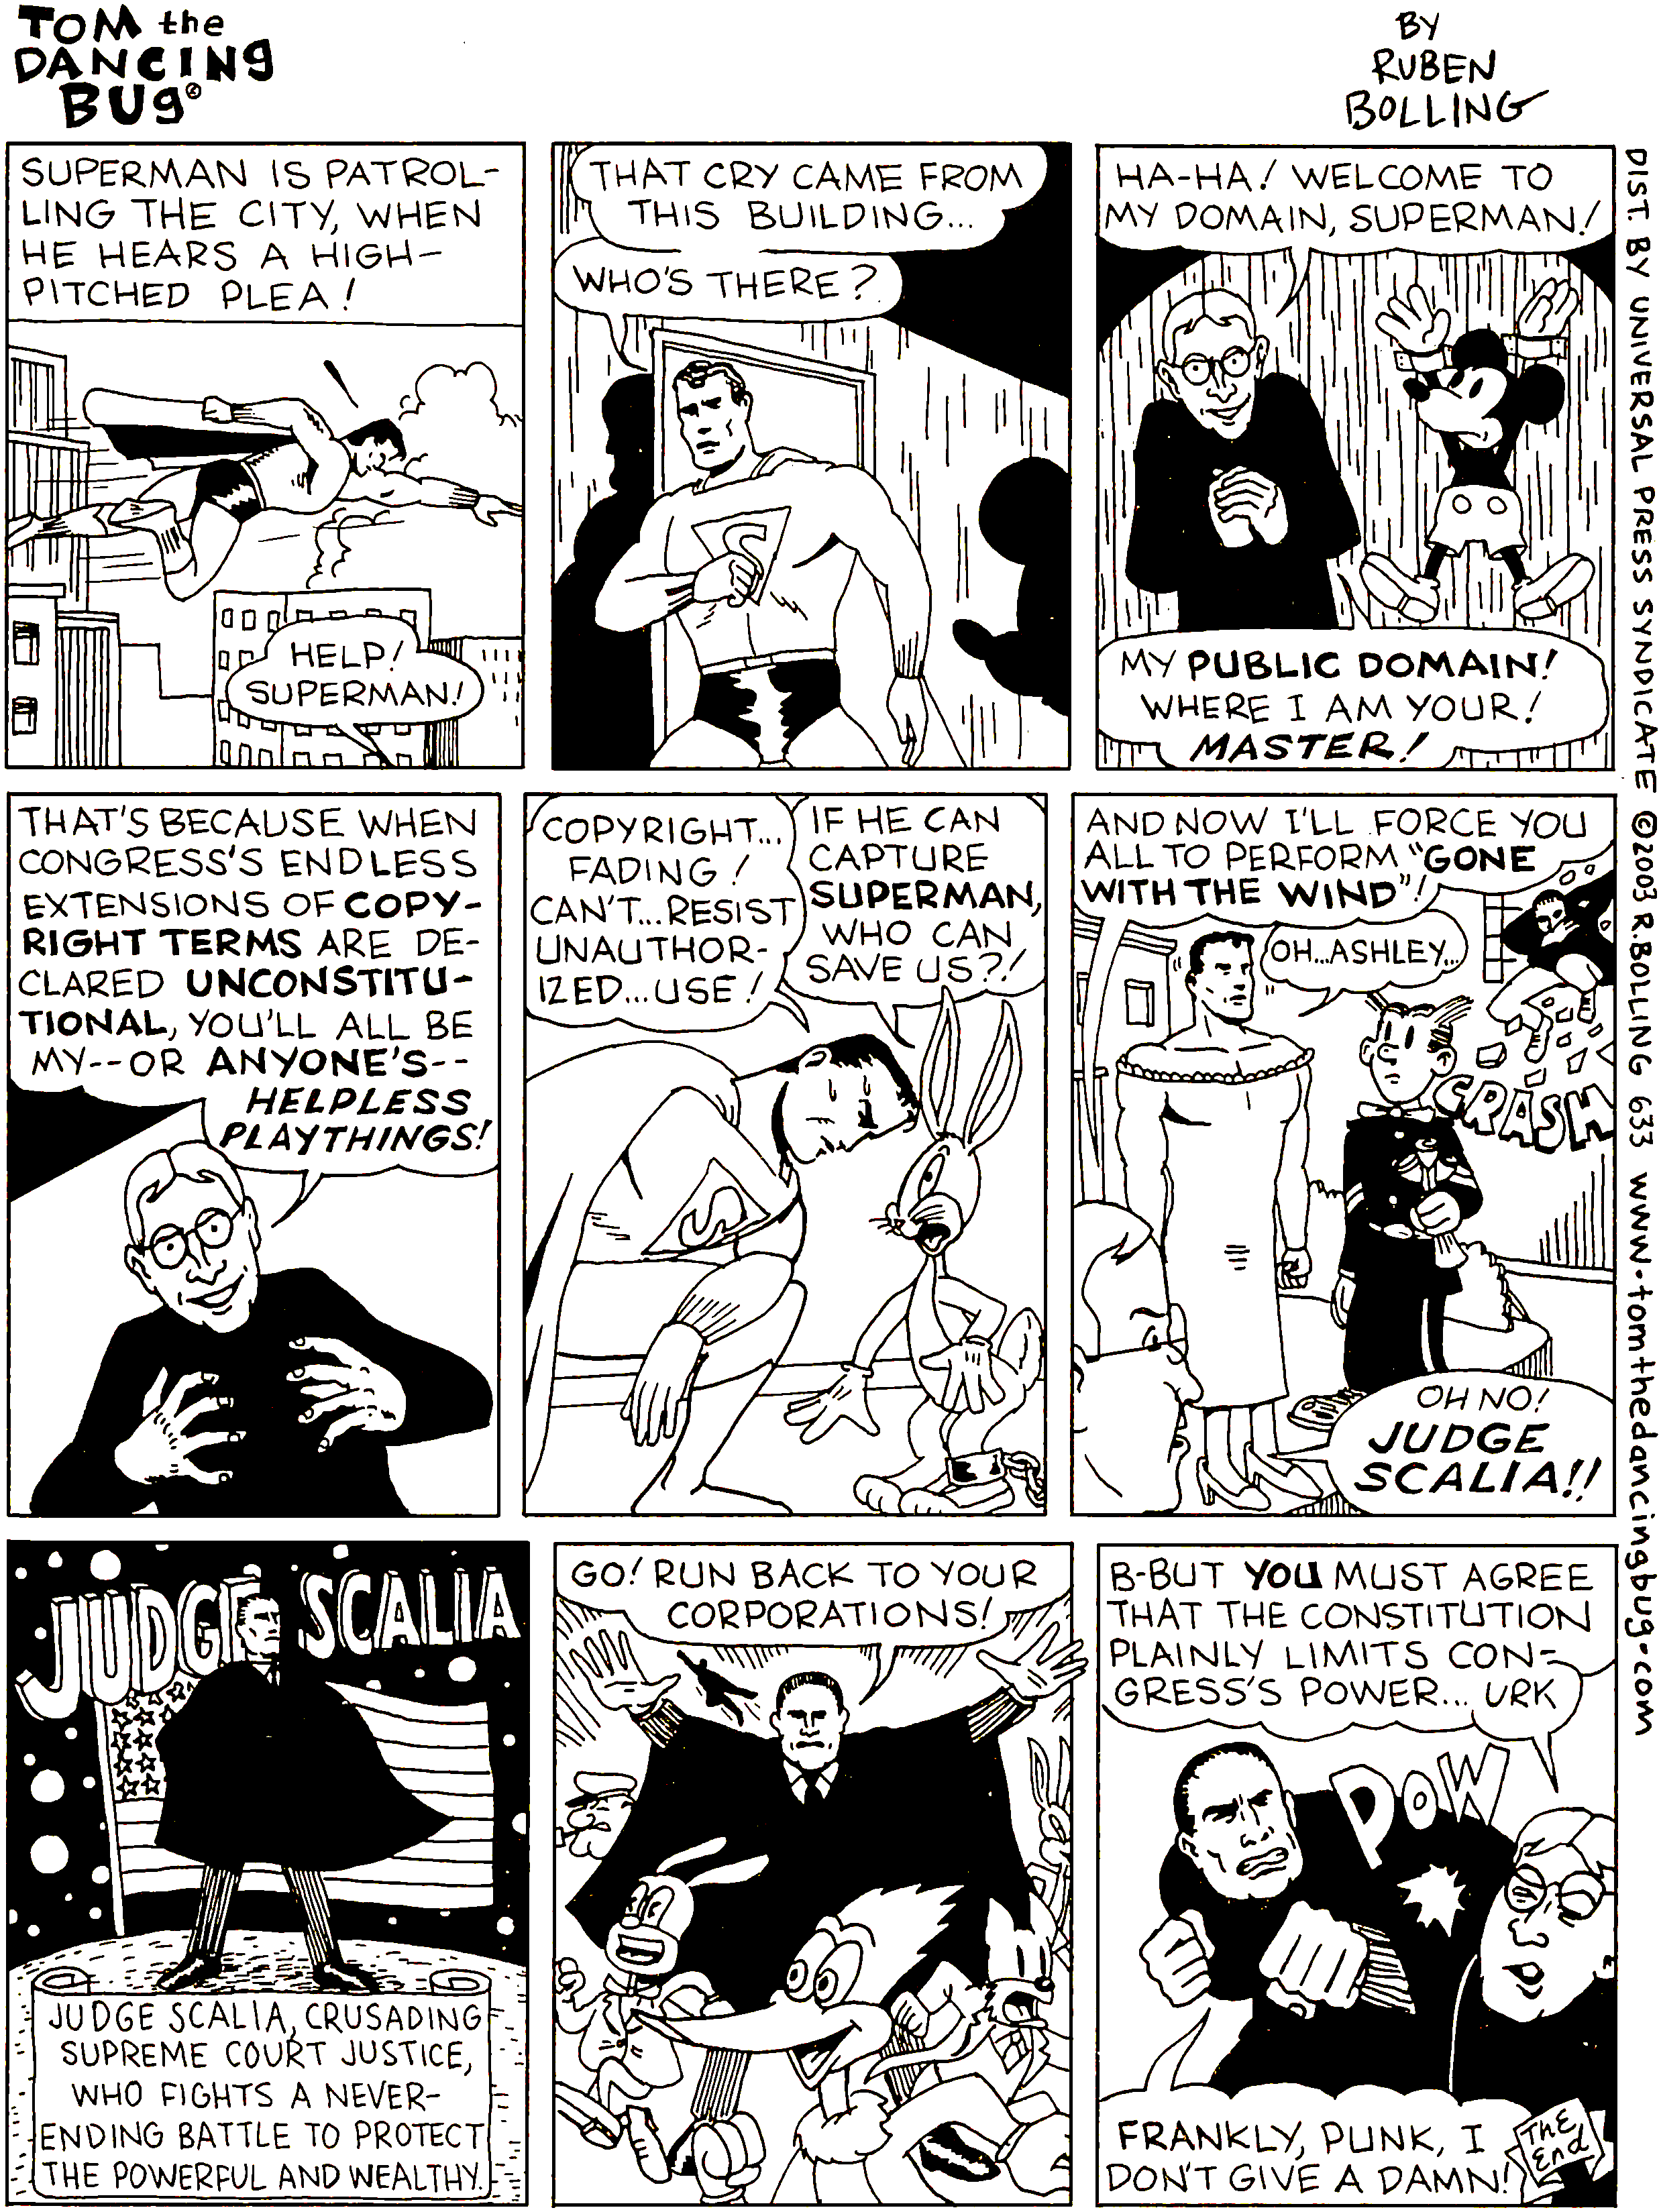
\includegraphics[width=1\linewidth,keepaspectratio=true]{images/tom-the-dancing-bug.png}}}}{[images/tom-{}the-{}dancing-{}bug.png not found]}\index{Bolling, Ruben}
\end{center}
\addtocounter{figure}{-1}\caption{}
\end{figure}

 The image that will always stick in my head is that evoked by the
quote from \emph{The New York Times}. That «grand experiment» we call the
«public domain» is over? When I can make light of it, I think, «Honey,
I shrunk the Constitution.» But I can rarely make light of it. We had
in our Constitution a commitment to free culture. In the case that I
fathered, the Supreme Court effectively renounced that commitment. A
better lawyer would have made them see differently.


% ------- 
% Chapter 
% ------- 
\setcounter{chapter}{13}

\chapter{Chapter Fourteen: Eldred II}
\label{eldred-ii}\hyperlabel{eldred-ii}%

 \textbf{The day} \emph{Eldred} was decided, fate would have it that I
was to travel to Washington, D.C. (The day the rehearing petition in
\emph{Eldred} was denied—meaning the case was
really finally over—fate would have it that I was giving a
speech to technologists at Disney World.)  This was a particularly
long flight to my least favorite city. The drive into the city from
Dulles was delayed because of traffic, so I opened up my computer and
wrote an op-{}ed piece.

\index{Ayer, Don}

 It was an act of contrition. During the whole of the flight from San
Francisco to Washington, I had heard over and over again in my head
the same advice from Don Ayer: You need to make them see why it is
important. And alternating with that command was the question of
Justice Kennedy: «For all these years the act has impeded progress in
science and the useful arts. I just don't see any empirical evidence for
that.» And so, having failed in the argument of constitutional principle,
finally, I turned to an argument of politics.


 \emph{The New York Times} published the piece. In it, I proposed a simple
fix: Fifty years after a work has been published, the copyright owner
 would be required to register the work and pay a small fee. If he paid
the fee, he got the benefit of the full term of copyright. If he did not,
the work passed into the public domain.


 We called this the Eldred Act, but that was just to give it a name.
Eric Eldred was kind enough to let his name be used once again, but as
he said early on, it won't get passed unless it has another name.


 Or another two names. For depending upon your perspective, this
is either the «Public Domain Enhancement Act» or the «Copyright
Term Deregulation Act.» Either way, the essence of the idea is clear
and obvious: Remove copyright where it is doing nothing except
blocking access and the spread of knowledge. Leave it for as long as
Congress allows for those works where its worth is at least \$1. But for
everything else, let the content go.

\index{Forbes, Steve}

 The reaction to this idea was amazingly strong. Steve Forbes endorsed
it in an editorial. I received an avalanche of e-{}mail and letters
expressing support. When you focus the issue on lost creativity,
people can see the copyright system makes no sense. As a good
Republican might say, here government regulation is simply getting in
the way of innovation and creativity. And as a good Democrat might
say, here the government is blocking access and the spread of
knowledge for no good reason. Indeed, there is no real difference
between Democrats and Republicans on this issue. Anyone can recognize
the stupid harm of the present system.


 Indeed, many recognized the obvious benefit of the registration
requirement.  For one of the hardest things about the current system
for people who want to license content is that there is no obvious
place to look for the current copyright owners. Since registration is
not required, since marking content is not required, since no
formality at all is required, it is often impossibly hard to locate
copyright owners to ask permission to use or license their work. This
system would lower these costs, by establishing at least one registry
where copyright owners could be identified.

\index{Berlin Act (1908)}\index{Berne Convention (1908)}

  As I described in chapter \ref{property-i} [\pageref{property-i}], formalities in copyright law were
removed in 1976, when Congress followed the Europeans by abandoning
any formal requirement before a copyright is granted.\footnote{
  \index{German copyright law} Until the 1908 Berlin Act of the Berne Convention, national copyright
legislation sometimes made protection depend upon compliance with
formalities such as registration, deposit, and affixation of notice of
the author's claim of copyright. However, starting with the 1908 act,
every text of the Convention has provided that «the enjoyment and the
exercise» of rights guaranteed by the Convention «shall not be subject
to any formality.»  The prohibition against formalities is presently
embodied in Article 5(2) of the Paris Text of the Berne
Convention. Many countries continue to impose some form of deposit or
registration requirement, albeit not as a condition of
copyright. French law, for example, requires the deposit of copies of
works in national repositories, principally the National Museum.
Copies of books published in the United Kingdom must be deposited in
the British Library. The German Copyright Act provides for a Registrar
of Authors where the author's true name can be filed in the case of
anonymous or pseudonymous works. Paul Goldstein, \emph{International
Intellectual Property Law, Cases and Materials} (New York: Foundation
Press, 2001), 153–54.  
} The Europeans are said to view copyright as a «natural right.» Natural
rights don't need forms to exist. Traditions, like the Anglo-{}American
tradition that required copyright owners to follow form if their
rights were to be protected, did not, the Europeans thought, properly
respect the dignity of the author. My right as a creator turns on my
creativity, not upon the special favor of the government.


 That's great rhetoric. It sounds wonderfully romantic. But it is
absurd copyright policy. It is absurd especially for authors, because
a world without formalities harms the creator. The ability to spread
«Walt Disney creativity» is destroyed when there is no simple way to
know what's protected and what's not.

\index{Berne Convention (1908)}

 The fight against formalities achieved its first real victory in
Berlin in 1908. International copyright lawyers amended the Berne
Convention in 1908, to require copyright terms of life plus fifty
years, as well as the abolition of copyright formalities. The
formalities were hated because the stories of inadvertent loss were
increasingly common. It was as if a Charles Dickens character ran all
copyright offices, and the failure to dot an \emph{i} or cross a
\emph{t} resulted in the loss of widows' only income.


 These complaints were real and sensible. And the strictness of the
formalities, especially in the United States, was absurd. The law
should always have ways of forgiving innocent mistakes. There is no
reason copyright law couldn't, as well. Rather than abandoning
formalities totally, the response in Berlin should have been to
embrace a more equitable system of registration.


 Even that would have been resisted, however, because registration
in the nineteenth and twentieth centuries was still expensive. It was
also a hassle. The abolishment of formalities promised not only to save
the starving widows, but also to lighten an unnecessary regulatory 
		burden
imposed upon creators.


 In addition to the practical complaint of authors in 1908, there was
a moral claim as well. There was no reason that creative property
  should be a second-{}class form of property. If a carpenter builds a
table, his rights over the table don't depend upon filing a form with
the government.  He has a property right over the table «naturally,» and he can assert that right against anyone who would steal the table,
whether or not he has informed the government of his ownership of the
table.


 This argument is correct, but its implications are misleading. For the
argument in favor of formalities does not depend upon creative
property being second-{}class property. The argument in favor of
formalities turns upon the special problems that creative property
presents.  The law of formalities responds to the special physics of
creative property, to assure that it can be efficiently and fairly
spread.


 No one thinks, for example, that land is second-{}class property just
because you have to register a deed with a court if your sale of land
is to be effective. And few would think a car is second-{}class property
just because you must register the car with the state and tag it with
a license.  In both of those cases, everyone sees that there is an
important reason to secure registration—both because it makes
the markets more efficient and because it better secures the rights of
the owner. Without a registration system for land, landowners would
perpetually have to guard their property. With registration, they can
simply point the police to a deed. Without a registration system for
cars, auto theft would be much easier. With a registration system, the
thief has a high burden to sell a stolen car. A slight burden is
placed on the property owner, but those burdens produce a much better
system of protection for property generally.


 It is similarly special physics that makes formalities important in
copyright law. Unlike a carpenter's table, there's nothing in nature that
makes it relatively obvious who might own a particular bit of creative
property. A recording of Lyle Lovett's latest album can exist in a billion
places without anything necessarily linking it back to a particular
owner. And like a car, there's no way to buy and sell creative property
with confidence unless there is some simple way to authenticate who is
the author and what rights he has. Simple transactions are destroyed in
  a world without formalities. Complex, expensive,
\emph{lawyer} transactions take their place.
\index{Lovett, Lyle} 

 This was the understanding of the problem with the Sonny Bono
Act that we tried to demonstrate to the Court. This was the part it
didn't «get.» Because we live in a system without formalities, there is no
way easily to build upon or use culture from our past. If copyright
terms were, as Justice Story said they would be, «short,» then this
wouldn't matter much. For fourteen years, under the framers' system, a
work would be presumptively controlled. After fourteen years, it would
be presumptively uncontrolled.


 But now that copyrights can be just about a century long, the
inability to know what is protected and what is not protected becomes
a huge and obvious burden on the creative process. If the only way a
library can offer an Internet exhibit about the New Deal is to hire a
lawyer to clear the rights to every image and sound, then the
copyright system is burdening creativity in a way that has never been
seen before \emph{because there are no formalities}.


 The Eldred Act was designed to respond to exactly this problem. If
it is worth \$1 to you, then register your work and you can get the
longer term. Others will know how to contact you and, therefore, how
to get your permission if they want to use your work. And you will get
the benefit of an extended copyright term.


 If it isn't worth it to you to register to get the benefit of an extended
term, then it shouldn't be worth it for the government to defend your
monopoly over that work either. The work should pass into the public
domain where anyone can copy it, or build archives with it, or create a
movie based on it. It should become free if it is not worth \$1 to you.


 Some worry about the burden on authors. Won't the burden of
registering the work mean that the \$1 is really misleading? Isn't the
hassle worth more than \$1? Isn't that the real problem with
registration?


 It is. The hassle is terrible. The system that exists now is awful. I
completely agree that the Copyright Office has done a terrible job (no
doubt because they are terribly funded) in enabling simple and cheap
  registrations. Any real solution to the problem of formalities must
address the real problem of \emph{governments} standing
at the core of any system of formalities. In this book, I offer such a
solution. That solution essentially remakes the Copyright Office. For
now, assume it was Amazon that ran the registration system. Assume it
was one-{}click registration.  The Eldred Act would propose a simple,
one-{}click registration fifty years after a work was published. Based
upon historical data, that system would move up to 98 percent of
commercial work, commercial work that no longer had a commercial life,
into the public domain within fifty years. What do you think?

\index{Forbes, Steve}

 \textbf{When Steve Forbes} endorsed the
idea, some in Washington began to pay attention. Many people contacted
me pointing to representatives who might be willing to introduce the
Eldred Act. And I had a few who directly suggested that they might be
willing to take the first step.

\index{Lofgren, Zoe}

 One representative, Zoe Lofgren of California, went so far as to get
the bill drafted. The draft solved any problem with international
law. It imposed the simplest requirement upon copyright owners
possible. In May 2003, it looked as if the bill would be
introduced. On May 16, I posted on the Eldred Act blog, «we are
close.» There was a general reaction in the blog community that
something good might happen here.


 But at this stage, the lobbyists began to intervene. Jack Valenti and
the MPAA general counsel came to the congresswoman's office to give
the view of the MPAA. Aided by his lawyer, as Valenti told me, Valenti
informed the congresswoman that the MPAA would oppose the Eldred
Act. The reasons are embarrassingly thin. More importantly, their
thinness shows something clear about what this debate is really about.


 The MPAA argued first that Congress had «firmly rejected the central
concept in the proposed bill»—that copyrights be renewed. That
was true, but irrelevant, as Congress's «firm rejection» had occurred
 long before the Internet made subsequent uses much more likely.
Second, they argued that the proposal would harm poor copyright
owners—apparently those who could not afford the \$1 fee. Third,
they argued that Congress had determined that extending a copyright
term would encourage restoration work. Maybe in the case of the small
percentage of work covered by copyright law that is still commercially
valuable, but again this was irrelevant, as the proposal would not cut
off the extended term unless the \$1 fee was not paid. Fourth, the MPAA
argued that the bill would impose «enormous» costs, since a
registration system is not free. True enough, but those costs are
certainly less than the costs of clearing the rights for a copyright
whose owner is not known. Fifth, they worried about the risks if the
copyright to a story underlying a film were to pass into the public
domain. But what risk is that? If it is in the public domain, then the
film is a valid derivative use.


 Finally, the MPAA argued that existing law enabled copyright owners to
do this if they wanted. But the whole point is that there are
thousands of copyright owners who don't even know they have a
copyright to give. Whether they are free to give away their copyright
or not—a controversial claim in any case—unless they know
about a copyright, they're not likely to.


 \textbf{At the beginning} of this book, I
told two stories about the law reacting to changes in technology. In
the one, common sense prevailed.  In the other, common sense was
delayed. The difference between the two stories was the power of the
opposition—the power of the side that fought to defend the
status quo. In both cases, a new technology threatened old
interests. But in only one case did those interest's have the power to
protect themselves against this new competitive threat.


 I used these two cases as a way to frame the war that this book has
been about. For here, too, a new technology is forcing the law to react.
And here, too, we should ask, is the law following or resisting common
sense? If common sense supports the law, what explains this common
sense?


   When the issue is piracy, it is right for the law to back the
copyright owners. The commercial piracy that I described is wrong and
harmful, and the law should work to eliminate it. When the issue is
p2p sharing, it is easy to understand why the law backs the owners
still: Much of this sharing is wrong, even if much is harmless. When
the issue is copyright terms for the Mickey Mouses of the world, it is
possible still to understand why the law favors Hollywood: Most people
don't recognize the reasons for limiting copyright terms; it is thus
still possible to see good faith within the resistance.

\index{Kelly, Kevin}

 But when the copyright owners oppose a proposal such as the Eldred
Act, then, finally, there is an example that lays bare the naked
selfinterest driving this war. This act would free an extraordinary
range of content that is otherwise unused. It wouldn't interfere with
any copyright owner's desire to exercise continued control over his
content. It would simply liberate what Kevin Kelly calls the «Dark
Content» that fills archives around the world. So when the warriors
oppose a change like this, we should ask one simple question:


 What does this industry really want?


 With very little effort, the warriors could protect their content. So
the effort to block something like the Eldred Act is not really about
protecting \emph{their} content. The effort to block the
Eldred Act is an effort to assure that nothing more passes into the
public domain. It is another step to assure that the public domain
will never compete, that there will be no use of content that is not
commercially controlled, and that there will be no commercial use of
content that doesn't require \emph{their} permission
first.


 The opposition to the Eldred Act reveals how extreme the other side
is. The most powerful and sexy and well loved of lobbies really has as
its aim not the protection of «property» but the rejection of a
tradition.  Their aim is not simply to protect what is
theirs. \emph{Their aim is to assure that all there is is what is
theirs}.


 It is not hard to understand why the warriors take this view. It is not
hard to see why it would benefit them if the competition of the public
  domain tied to the Internet could somehow be quashed. Just as RCA
feared the competition of FM, they fear the competition of a public
domain connected to a public that now has the means to create with it
and to share its own creation.

\index{Causby, Thomas Lee}\index{Causby, Tinie}

 What is hard to understand is why the public takes this view. It is
as if the law made airplanes trespassers. The MPAA stands with the
Causbys and demands that their remote and useless property rights be
respected, so that these remote and forgotten copyright holders might
block the progress of others.


 All this seems to follow easily from this untroubled acceptance of the
«property» in intellectual property. Common sense supports it, and so
long as it does, the assaults will rain down upon the technologies of
the Internet. The consequence will be an increasing «permission
society.»  The past can be cultivated only if you can identify the
owner and gain permission to build upon his work. The future will be
controlled by this dead (and often unfindable) hand of the past.

\bookmarksetup{startatroot}

% ------------------ 
% Unnumbered Chapter 
% ------------------ 
\setcounter{secnumdepth}{-1}

\chapter{Conclusion}
\label{c-conclusion}\hyperlabel{c-conclusion}%
\index{Africa, medications for HIV patients in|(}\index{AIDS medications|(}\index{antiretroviral drugs|(}\index{developing countries, foreign patent costs in|(}\index{drugs!pharmaceutical|(}\index{HIV/AIDS therapies|(}

 \textbf{There are more} than 35 million
people with the AIDS virus worldwide. Twenty-{}five million of them live
in sub-{}Saharan Africa.  Seventeen million have already died. Seventeen
million Africans is proportional percentage-{}wise to seven million
Americans. More importantly, it is seventeen million Africans.


 There is no cure for AIDS, but there are drugs to slow its
progression.  These antiretroviral therapies are still experimental,
but they have already had a dramatic effect. In the United States,
AIDS patients who regularly take a cocktail of these drugs increase
their life expectancy by ten to twenty years. For some, the drugs make
the disease almost invisible.


 These drugs are expensive. When they were first introduced in the
United States, they cost between \$10,000 and \$15,000 per person per
year. Today, some cost \$25,000 per year. At these prices, of course, no
African nation can afford the drugs for the vast majority of its 
		population:
\$15,000 is thirty times the per capita gross national product of
Zimbabwe. At these prices, the drugs are totally unavailable.\footnote{
  Commission on Intellectual Property Rights, «Final Report: Integrating
Intellectual Property Rights and Development Policy» (London, 2002),
available at 
\href{http://free-culture.cc/notes/}{link \#55}. According to a World Health Organization press 
		release
issued 9 July 2002, only 230,000 of the 6 million who need drugs in
the developing world receive them—and half of them are in Brazil.

} 
\index{patents!on pharmaceuticals|(}\index{pharmaceutical patents|(}

  These prices are not high because the ingredients of the drugs are
expensive. These prices are high because the drugs are protected by
patents. The drug companies that produced these life-{}saving mixes
enjoy at least a twenty-{}year monopoly for their inventions. They use
that monopoly power to extract the most they can from the market. That
power is in turn used to keep the prices high.


 There are many who are skeptical of patents, especially drug
patents. I am not. Indeed, of all the areas of research that might be
supported by patents, drug research is, in my view, the clearest case
where patents are needed. The patent gives the drug company some
assurance that if it is successful in inventing a new drug to treat a
disease, it will be able to earn back its investment and more. This is
socially an extremely valuable incentive. I am the last person who
would argue that the law should abolish it, at least without other
changes.


 But it is one thing to support patents, even drug patents. It is
another thing to determine how best to deal with a crisis. And as
African leaders began to recognize the devastation that AIDS was
bringing, they started looking for ways to import HIV treatments at
costs significantly below the market price.

\index{international law|(}\index{parallel importation|(}\index{South Africa, Republic of, pharmaceutical imports by|(}

 In 1997, South Africa tried one tack. It passed a law to allow the
importation of patented medicines that had been produced or sold in
another nation's market with the consent of the patent owner. For
example, if the drug was sold in India, it could be imported into
Africa from India. This is called «parallel importation,» and it is
generally permitted under international trade law and is specifically
permitted within the European Union.\footnote{
  See Peter Drahos with John Braithwaite, \emph{Information Feudalism: Who
Owns the Knowledge Economy?} (New York: The New Press, 2003), 37.
\index{Braithwaite, John} \index{Drahos, Peter} 
} 
\index{United States Trade Representative (USTR)}

 However, the United States government opposed the bill. Indeed, more
than opposed. As the International Intellectual Property Association
characterized it, «The U.S. government pressured South Africa …
not to permit compulsory licensing or parallel
imports.»\footnote{
  International Intellectual Property Institute (IIPI), \emph{Patent
Protection and Access to HIV/AIDS Pharmaceuticals in Sub-{}Saharan
Africa, a Report Prepared for the World Intellectual Property
Organization} (Washington, D.C., 2000), 14, available at
\href{http://free-culture.cc/notes/}{link \#56}. For a
firsthand account of the struggle over South Africa, see Hearing
Before the Subcommittee on Criminal Justice, Drug Policy, and Human
Resources, House Committee on Government Reform, H. Rep., 1st sess.,
Ser. No. 106-{}126 (22 July 1999), 150–57 (statement of James
Love).

} Through the Office of the United States Trade Representative, the
government asked South Africa to change the law—and to add
pressure to that request, in 1998, the USTR listed South Africa for
possible trade sanctions.
 That same year, more than forty pharmaceutical companies began
proceedings in the South African courts to challenge the government's
actions. The United States was then joined by other governments from
the EU. Their claim, and the claim of the pharmaceutical companies,
was that South Africa was violating its obligations under
international law by discriminating against a particular kind of
patent— pharmaceutical patents. The demand of these governments,
with the United States in the lead, was that South Africa respect
these patents as it respects any other patent, regardless of any
effect on the treatment of AIDS within South Africa.\footnote{
  International Intellectual Property Institute (IIPI), \emph{Patent
Protection and Access to HIV/AIDS Pharmaceuticals in Sub-{}Saharan
Africa, a Report Prepared for the World Intellectual Property
Organization} (Washington, D.C., 2000), 15.  
} 
\index{parallel importation|)}
 We should place the intervention by the United States in context.  No
doubt patents are not the most important reason that Africans don't
have access to drugs. Poverty and the total absence of an effective
health care infrastructure matter more. But whether patents are the
most important reason or not, the price of drugs has an effect on
their demand, and patents affect price. And so, whether massive or
marginal, there was an effect from our government's intervention to
stop the flow of medications into Africa.


 By stopping the flow of HIV treatment into Africa, the United
States government was not saving drugs for United States citizens.
This is not like wheat (if they eat it, we can't); instead, the flow that the
United States intervened to stop was, in effect, a flow of knowledge:
information about how to take chemicals that exist within Africa, and
turn those chemicals into drugs that would save 15 to 30 million lives.


 Nor was the intervention by the United States going to protect the
profits of United States drug companies—at least, not substantially. It
was not as if these countries were in the position to buy the drugs for
the prices the drug companies were charging. Again, the Africans are
wildly too poor to afford these drugs at the offered prices. Stopping the
parallel import of these drugs would not substantially increase the sales
by U.S. companies.


 Instead, the argument in favor of restricting this flow of
information, which was needed to save the lives of millions, was an
argument
 about the sanctity of property.\footnote{
  See Sabin Russell, «New Crusade to Lower AIDS Drug Costs: Africa's
Needs at Odds with Firms' Profit Motive,» \emph{San Francisco Chronicle}, 24
May 1999, A1, available at
\href{http://free-culture.cc/notes/}{link \#57} («compulsory licenses and gray markets pose a threat to the entire
system of intellectual property protection»); Robert Weissman, «AIDS
and Developing Countries: Democratizing Access to Essential
Medicines,» \emph{Foreign Policy in Focus} 4:23 (August 1999), available at
\href{http://free-culture.cc/notes/}{link \#58} (describing U.S. policy); John A. Harrelson, «TRIPS, Pharmaceutical
Patents, and the HIV/AIDS Crisis: Finding the Proper Balance Between
Intellectual Property Rights and Compassion, a Synopsis,» \emph{Widener Law
Symposium Journal} (Spring 2001): 175.
 
} It was because «intellectual property» would be violated that these
drugs should not flow into Africa. It was a principle about the
importance of «intellectual property» that led these government actors
to intervene against the South African response to AIDS.

\index{South Africa, Republic of, pharmaceutical imports by|)}

 Now just step back for a moment. There will be a time thirty years
from now when our children look back at us and ask, how could we have
let this happen? How could we allow a policy to be pursued whose
direct cost would be to speed the death of 15 to 30 million Africans,
and whose only real benefit would be to uphold the «sanctity» of an
idea?  What possible justification could there ever be for a policy
that results in so many deaths? What exactly is the insanity that
would allow so many to die for such an abstraction?

\index{corporations!in pharmaceutical industry|(}

 Some blame the drug companies. I don't. They are corporations.
Their managers are ordered by law to make money for the corporation.
They push a certain patent policy not because of ideals, but because it is
the policy that makes them the most money. And it only makes them the
most money because of a certain corruption within our political system—
a corruption the drug companies are certainly not responsible for.


 The corruption is our own politicians' failure of integrity. For the
drug companies would love—they say, and I believe them—to
sell their drugs as cheaply as they can to countries in Africa and
elsewhere.  There are issues they'd have to resolve to make sure the
drugs didn't get back into the United States, but those are mere
problems of technology.  They could be overcome.

\index{intellectual property rights!of drug patents|(}

 A different problem, however, could not be overcome. This is the
fear of the grandstanding politician who would call the presidents of
the drug companies before a Senate or House hearing, and ask, «How
is it you can sell this HIV drug in Africa for only \$1 a pill, but the same
drug would cost an American \$1,500?» Because there is no «sound
bite» answer to that question, its effect would be to induce regulation
of prices in America. The drug companies thus avoid this spiral by
avoiding the first step. They reinforce the idea that property should be
 sacred. They adopt a rational strategy in an irrational context, with the
unintended consequence that perhaps millions die. And that rational
strategy thus becomes framed in terms of this ideal—the sanctity of an
idea called «intellectual property.» 
\index{Africa, medications for HIV patients in|)}\index{AIDS medications|)}\index{antiretroviral drugs|)}\index{developing countries, foreign patent costs in|)}\index{drugs!pharmaceutical|)}\index{HIV/AIDS therapies|)}
\index{corporations!in pharmaceutical industry|)}

 So when the common sense of your child confronts you, what will
you say? When the common sense of a generation finally revolts
against what we have done, how will we justify what we have done?
What is the argument?


 A sensible patent policy could endorse and strongly support the patent
system without having to reach everyone everywhere in exactly the same
way. Just as a sensible copyright policy could endorse and strongly
support a copyright system without having to regulate the spread of
culture perfectly and forever, a sensible patent policy could endorse
and strongly support a patent system without having to block the
spread of drugs to a country not rich enough to afford market prices
in any case. A sensible policy, in other words, could be a balanced
policy. For most of our history, both copyright and patent policies
were balanced in just this sense.

\index{patents!on pharmaceuticals|)}\index{pharmaceutical patents|)}
\index{international law|)}
 But we as a culture have lost this sense of balance. We have lost the
critical eye that helps us see the difference between truth and
extremism.  A certain property fundamentalism, having no connection to
our tradition, now reigns in this culture—bizarrely, and with
consequences more grave to the spread of ideas and culture than almost
any other single policy decision that we as a democracy will make.

\index{intellectual property rights!of drug patents|)}

 \textbf{A simple idea} blinds us, and under
the cover of darkness, much happens that most of us would reject if
any of us looked. So uncritically do we accept the idea of property in
ideas that we don't even notice how monstrous it is to deny ideas to a
people who are dying without them. So uncritically do we accept the
idea of property in culture that we don't even question when the
control of that property removes our
 ability, as a people, to develop our culture democratically. Blindness
becomes our common sense. And the challenge for anyone who would
reclaim the right to cultivate our culture is to find a way to make
this common sense open its eyes.


 So  far, common sense sleeps. There is no revolt. Common sense
does not yet see what there could be to revolt about. The extremism
that now dominates this debate fits with ideas that seem natural, and
that fit is reinforced by the RCAs of our day. They wage a frantic war
to fight «piracy,» and devastate a culture for creativity. They defend
the idea of «creative property,» while transforming real creators into
modern-{}day sharecroppers. They are insulted by the idea that rights
should be balanced, even though each of the major players in this
content war was itself a beneficiary of a more balanced ideal. The
hypocrisy reeks. Yet in a city like Washington, hypocrisy is not even
noticed. Powerful lobbies, complex issues, and MTV attention spans
produce the «perfect storm» for free culture.

\index{academic journals}\index{biomedical research}\index{intellectual property rights!international organization on issues of|(}\index{Internet!development of}\index{IBM}\index{PLoS (Public Library of Science)}\index{Public Library of Science (PLoS)}\index{public domain!public projects in}\index{single nucleotied polymorphisms (SNPs)}\index{Wellcome Trust}\index{World Intellectual Property Organization (WIPO)|(}\index{World Wide Web}\index{Global Positioning System}\index{Reagan, Ronald}\index{biomedical research|(}

 \textbf{In August 2003}, a fight broke out
in the United States about a decision by the World Intellectual
Property Organization to cancel a meeting.\footnote{
  Jonathan Krim, «The Quiet War over Open-{}Source,» \emph{Washington Post},
August 2003, E1, available at 
\href{http://free-culture.cc/notes/}{link \#59}; William New, «Global Group's
Shift on \`{}Open Source' Meeting Spurs Stir,» \emph{National Journal's Technology
Daily}, 19 August 2003, available at 
\href{http://free-culture.cc/notes/}{link \#60}; William New, «U.S. Official
Opposes \`{}Open Source' Talks at WIPO,» \emph{National Journal's Technology
Daily}, 19 August 2003, available at 
\href{http://free-culture.cc/notes/}{link \#61}.

} At the request of a wide range of interests, WIPO had decided to hold
a meeting to discuss «open and collaborative projects to create public
goods.» These are projects that have been successful in producing
public goods without relying exclusively upon a proprietary use of
intellectual property. Examples include the Internet and the World
Wide Web, both of which were developed on the basis of protocols in
the public domain. It included an emerging trend to support open
academic journals, including the Public Library of Science project
that I describe in chapter 
\ref{c-afterword} [\pageref{c-afterword}].  It
included a project to develop single nucleotide polymorphisms (SNPs),
which are thought to have great significance in biomedical
research. (That nonprofit project comprised a consortium of the
Wellcome Trust and pharmaceutical and technological companies,
including Amersham Biosciences, AstraZeneca,
 Aventis, Bayer, Bristol-{}Myers Squibb, Hoffmann-{}La Roche,
Glaxo-{}SmithKline, IBM, Motorola, Novartis, Pfizer, and Searle.) It
included the Global Positioning System, which Ronald Reagan set free
in the early 1980s. And it included «open source and free software.» 
\index{biomedical research|)}

 The aim of the meeting was to consider this wide range of projects
from one common perspective: that none of these projects relied upon
intellectual property extremism. Instead, in all of them, intellectual
property was balanced by agreements to keep access open or to impose
limitations on the way in which proprietary claims might be used.

\index{Lessig, Lawrence!in international debate on intellectual property|(}

 From the perspective of this book, then, the conference was ideal.\footnote{
  I should disclose that I was one of the people who asked WIPO for the
meeting.

} The projects within its scope included both commercial and
noncommercial work. They primarily involved science, but from many
perspectives.  And WIPO was an ideal venue for this discussion, since
WIPO is the preeminent international body dealing with intellectual
property issues.

\index{World Summit on the Information Society (WSIS)|(}

 Indeed, I was once publicly scolded for not recognizing this fact
about WIPO. In February 2003, I delivered a keynote address to a
preparatory conference for the World Summit on the Information Society
(WSIS). At a press conference before the address, I was asked what I
would say. I responded that I would be talking a little about the
importance of balance in intellectual property for the development of
an information society. The moderator for the event then promptly
interrupted to inform me and the assembled reporters that no question
about intellectual property would be discussed by WSIS, since those
questions were the exclusive domain of WIPO. In the talk that I had
prepared, I had actually made the issue of intellectual property
relatively minor. But after this astonishing statement, I made
intellectual property the sole focus of my talk. There was no way to
talk about an «Information Society» unless one also talked about the
range of information and culture that would be free. My talk did not
make my immoderate moderator very happy. And she was no doubt correct
that the scope of intellectual property protections was ordinarily the
stuff of
 WIPO. But in my view, there couldn't be too much of a conversation
about how much intellectual property is needed, since in my view, the
very idea of balance in intellectual property had been lost.


 So whether or not WSIS can discuss balance in intellectual property, I
had thought it was taken for granted that WIPO could and should. And
thus the meeting about «open and collaborative projects to create
public goods» seemed perfectly appropriate within the WIPO agenda.

\index{intellectual property rights!international organization on issues of|)}\index{World Intellectual Property Organization (WIPO)|)}\index{World Summit on the Information Society (WSIS)|)}
\index{free software/open-{}source software (FS/OSS)|(}\index{Apple Corporation}\index{Microsoft!on free software|(}

 But there is one project within that list that is highly
controversial, at least among lobbyists. That project is «open source
and free software.»  Microsoft in particular is wary of discussion of
the subject. From its perspective, a conference to discuss open source
and free software would be like a conference to discuss Apple's
operating system. Both open source and free software compete with
Microsoft's software. And internationally, many governments have begun
to explore requirements that they use open source or free software,
rather than «proprietary software,» for their own internal uses.

\index{copyleft licenses}\index{GNU/Linux operating system}\index{Linux operating system}\index{IBM}

 I don't mean to enter that debate here. It is important only to
make clear that the distinction is not between commercial and
noncommercial software. There are many important companies that depend
fundamentally upon open source and free software, IBM being the most
prominent. IBM is increasingly shifting its focus to the GNU/Linux
operating system, the most famous bit of «free software»—and IBM
is emphatically a commercial entity. Thus, to support «open source and
free software» is not to oppose commercial entities. It is, instead,
to support a mode of software development that is different from
Microsoft's.\footnote{
  Microsoft's position about free and open source software is more
sophisticated.  As it has repeatedly asserted, it has no problem with
«open source» software or software in the public domain. Microsoft's
principal opposition is to «free software» licensed under a «copyleft» license, meaning a license that requires the licensee to adopt the
same terms on any derivative work. See Bradford L. Smith, «The Future
of Software: Enabling the Marketplace to Decide,» \emph{Government Policy
Toward Open Source Software} (Washington, D.C.: AEI-{}Brookings Joint
Center for Regulatory Studies, American Enterprise Institute for
Public Policy Research, 2002), 69, available at
\href{http://free-culture.cc/notes/}{link \#62}. See also
Craig Mundie, Microsoft senior vice president, \emph{The Commercial Software
Model}, discussion at New York University Stern School of Business (3
May 2001), available at
\href{http://free-culture.cc/notes/}{link \#63}.

} 
\index{Lessig, Lawrence!in international debate on intellectual property|)}
\index{General Public License (GPL)}\index{GPL (General Public License)}

 More important for our purposes, to support «open source and free
software» is not to oppose copyright. «Open source and free software» is not software in the public domain. Instead, like Microsoft's
software, the copyright owners of free and open source software insist
quite strongly that the terms of their software license be respected
by
 adopters of free and open source software. The terms of that license
are no doubt different from the terms of a proprietary software
license.  Free software licensed under the General Public License
(GPL), for example, requires that the source code for the software be
made available by anyone who modifies and redistributes the
software. But that requirement is effective only if copyright governs
software. If copyright did not govern software, then free software
could not impose the same kind of requirements on its adopters. It
thus depends upon copyright law just as Microsoft does.

\index{intellectual property rights!international organization on issues of|(}\index{World Intellectual Property Organization (WIPO)|(}\index{Krim, Jonathan|(}\index{Microsoft!WIPO meeting opposed by}

 It is therefore understandable that as a proprietary software
developer, Microsoft would oppose this WIPO meeting, and
understandable that it would use its lobbyists to get the United
States government to oppose it, as well. And indeed, that is just what
was reported to have happened. According to Jonathan Krim of the
\emph{Washington Post}, Microsoft's lobbyists succeeded in getting the United
States government to veto the meeting.\footnote{
  Krim, «The Quiet War over Open-{}Source,» available at \href{http://free-culture.cc/notes/}{link \#64}.

} And without U.S. backing, the meeting was canceled.


 I don't blame Microsoft for doing what it can to advance its own
interests, consistent with the law. And lobbying governments is
plainly consistent with the law. There was nothing surprising about
its lobbying here, and nothing terribly surprising about the most
powerful software producer in the United States having succeeded in
its lobbying efforts.

\index{Microsoft!on free software|)}
\index{Boland, Lois}

 What was surprising was the United States government's reason for
opposing the meeting. Again, as reported by Krim, Lois Boland, acting
director of international relations for the U.S. Patent and Trademark
Office, explained that «open-{}source software runs counter to the
mission of WIPO, which is to promote intellectual-{}property rights.» She is quoted as saying, «To hold a meeting which has as its purpose
to disclaim or waive such rights seems to us to be contrary to the
goals of WIPO.» 
\index{Krim, Jonathan|)}
 These statements are astonishing on a number of levels.

\index{free software/open-{}source software (FS/OSS)|)}
 First, they are just flat wrong. As I described, most open source and
free software relies fundamentally upon the intellectual property
right called «copyright».  Without it, restrictions imposed by those
licenses wouldn't work. Thus, to say it «runs counter» to the mission
of promoting intellectual property rights reveals an extraordinary gap
in understanding—the sort of mistake that is excusable in a
first-{}year law student, but an embarrassment from a high government
official dealing with intellectual property issues.

\index{World Summit on the Information Society (WSIS)}\index{drugs!pharmaceutical}\index{generic drugs}\index{patents!on pharmaceuticals}

 Second, who ever said that WIPO's exclusive aim was to «promote» intellectual property maximally? As I had been scolded at the
preparatory conference of WSIS, WIPO is to consider not only how best
to protect intellectual property, but also what the best balance of
intellectual property is. As every economist and lawyer knows, the
hard question in intellectual property law is to find that
balance. But that there should be limits is, I had thought,
uncontested. One wants to ask Ms. Boland, are generic drugs (drugs
based on drugs whose patent has expired) contrary to the WIPO mission?
Does the public domain weaken intellectual property? Would it have
been better if the protocols of the Internet had been patented?

\index{Gates, Bill}

 Third, even if one believed that the purpose of WIPO was to maximize
intellectual property rights, in our tradition, intellectual property
rights are held by individuals and corporations. They get to decide
what to do with those rights because, again, they are
\emph{their} rights. If they want to «waive» or
«disclaim» their rights, that is, within our tradition, totally
appropriate. When Bill Gates gives away more than \$20 billion to do
good in the world, that is not inconsistent with the objectives of the
property system. That is, on the contrary, just what a property system
is supposed to be about: giving individuals the right to decide what
to do with \emph{their} property.

\index{Boland, Lois|(}

 When Ms. Boland says that there is something wrong with a meeting
«which has as its purpose to disclaim or waive such rights,» she's
saying that WIPO has an interest in interfering with the choices of
 the individuals who own intellectual property rights. That somehow,
WIPO's objective should be to stop an individual from «waiving» or
«disclaiming» an intellectual property right. That the interest of
WIPO is not just that intellectual property rights be maximized, but
that they also should be exercised in the most extreme and restrictive
way possible.

\index{feudal system|(}\index{property rights!feudal system of|(}

 There is a history of just such a property system that is well known
in the Anglo-{}American tradition. It is called «feudalism.» Under
feudalism, not only was property held by a relatively small number of
individuals and entities. And not only were the rights that ran with
that property powerful and extensive. But the feudal system had a
strong interest in assuring that property holders within that system
not weaken feudalism by liberating people or property within their
control to the free market. Feudalism depended upon maximum control
and concentration. It fought any freedom that might interfere with
that control.

\index{Drahos, Peter}\index{Braithwaite, John}

 As Peter Drahos and John Braithwaite relate, this is precisely the
choice we are now making about intellectual property.\footnote{
  See Drahos with Braithwaite, \emph{Information Feudalism}, 210–20.
\index{Drahos, Peter} 
} We will have an information society. That much is certain. Our only
choice now is whether that information society will be
\emph{free} or \emph{feudal}. The trend is
toward the feudal.

\index{feudal system|)}\index{property rights!feudal system of|)}

 When this battle broke, I blogged it. A spirited debate within the
comment section ensued. Ms. Boland had a number of supporters who
tried to show why her comments made sense. But there was one comment
that was particularly depressing for me. An anonymous poster wrote,

\begin{quote}
\index{intellectual property rights!international organization on issues of|)}\index{World Intellectual Property Organization (WIPO)|)}
 George, you misunderstand Lessig: He's only talking about the world as
it should be («the goal of WIPO, and the goal of any government,
should be to promote the right balance of intellectual property rights,
not simply to promote intellectual property rights»), not as it is. If
we were talking about the world as it is, then of course Boland didn't
say anything wrong. But in the world
 as Lessig would have it, then of course she did. Always pay attention
to the distinction between Lessig's world and ours.


\end{quote}

 I missed the irony the first time I read it. I read it quickly and
thought the poster was supporting the idea that seeking balance was
what our government should be doing. (Of course, my criticism of Ms.
Boland was not about whether she was seeking balance or not; my
criticism was that her comments betrayed a first-{}year law student's
mistake. I have no illusion about the extremism of our government,
whether Republican or Democrat. My only illusion apparently is about
whether our government should speak the truth or not.)

\index{Boland, Lois|)}

 Obviously, however, the poster was not supporting that idea.  Instead,
the poster was ridiculing the very idea that in the real world, the
«goal» of a government should be «to promote the right balance» of
intellectual property. That was obviously silly to him. And it
obviously betrayed, he believed, my own silly utopianism. «Typical for
an academic,» the poster might well have continued.


 I understand criticism of academic utopianism. I think utopianism is
silly, too, and I'd be the first to poke fun at the absurdly
unrealistic ideals of academics throughout history (and not just in
our own country's history).


 But when it has become silly to suppose that the role of our
government should be to «seek balance,» then count me with the silly,
for that means that this has become quite serious indeed. If it should
be obvious to everyone that the government does not seek balance, that
the government is simply the tool of the most powerful lobbyists, that
the idea of holding the government to a different standard is absurd,
that the idea of demanding of the government that it speak truth and
not lies is just naïve, then who have we, the most powerful
democracy in the world, become?


 It might be crazy to expect a high government official to speak
the truth. It might be crazy to believe that government policy will be
something more than the handmaiden of the most powerful interests.
 It might be crazy to argue that we should preserve a tradition that has
been part of our tradition for most of our history—free culture.


 If this is crazy, then let there be more crazies. Soon.

\index{CodePink Women in Peace}\index{Safire, William}\index{Turner, Ted}

 \textbf{There are moments} of hope in this
struggle. And moments that surprise. When the FCC was considering
relaxing ownership rules, which would thereby further increase the
concentration in media ownership, an extraordinary bipartisan
coalition formed to fight this change. For perhaps the first time in
history, interests as diverse as the NRA, the ACLU, Moveon.org,
William Safire, Ted Turner, and CodePink Women for Peace organized to
oppose this change in FCC policy. An astonishing 700,000 letters were
sent to the FCC, demanding more hearings and a different result.


 This activism did not stop the FCC, but soon after, a broad coalition
in the Senate voted to reverse the FCC decision. The hostile hearings
leading up to that vote revealed just how powerful this movement had
become. There was no substantial support for the FCC's decision, and
there was broad and sustained support for fighting further
concentration in the media.


 But even this movement misses an important piece of the puzzle.
Largeness as such is not bad. Freedom is not threatened just because
some become very rich, or because there are only a handful of big
players.  The poor quality of Big Macs or Quarter Pounders does not
mean that you can't get a good hamburger from somewhere else.


 The danger in media concentration comes not from the concentration,
but instead from the feudalism that this concentration, tied to the
change in copyright, produces. It is not just that there are a few
powerful companies that control an ever expanding slice of the
media. It is that this concentration can call upon an equally bloated
range of rights—property rights of a historically extreme
form—that makes their bigness bad.


 It is therefore significant that so many would rally to demand
competition and increased diversity. Still, if the rally is understood
as being about bigness alone, it is not terribly surprising. We
Americans have a long history of fighting «big,» wisely or not. That
we could be motivated to fight «big» again is not something new.


 It would be something new, and something very important, if an equal
number could be rallied to fight the increasing extremism built within
the idea of «intellectual property.» Not because balance is alien to
our tradition; indeed, as I've argued, balance is our tradition. But
because the muscle to think critically about the scope of anything
called «property» is not well exercised within this tradition anymore.


 If we were Achilles, this would be our heel. This would be the place
of our tragedy.

\index{Dylan, Bob}

 \textbf{As I write} these final words, the
news is filled with stories about the RIAA lawsuits against almost
three hundred individuals.\footnote{
  John Borland, «RIAA Sues 261 File Swappers,» CNET News.com, September
2003, available at
\href{http://free-culture.cc/notes/}{link \#65}; Paul
R. La Monica, «Music Industry Sues Swappers,» CNN/Money, 8 September
2003, available at
\href{http://free-culture.cc/notes/}{link \#66}; Soni
Sangha and Phyllis Furman with Robert Gearty, «Sued for a Song,
N.Y.C. 12-{}Yr-{}Old Among 261 Cited as Sharers,» \emph{New York Daily News}, 9
September 2003, 3; Frank Ahrens, «RIAA's Lawsuits Meet Surprised
Targets; Single Mother in Calif., 12-{}Year-{}Old Girl in N.Y. Among
Defendants,» \emph{Washington Post}, 10 September 2003, E1; Katie Dean,
«Schoolgirl Settles with RIAA,» \emph{Wired News}, 10 September 2003,
available at
\href{http://free-culture.cc/notes/}{link \#67}.

} Eminem has just been sued for «sampling» someone else's
music.\footnote{
  Jon Wiederhorn, «Eminem Gets Sued … by a Little Old Lady,» mtv.com, 17 September 2003, available at
\href{http://free-culture.cc/notes/}{link \#68}.

} The story about Bob Dylan «stealing» from a Japanese author has just
finished making the rounds.\footnote{
  Kenji Hall, Associated Press, «Japanese Book May Be Inspiration for
Dylan Songs,» Kansascity.com, 9 July 2003, available at
\href{http://free-culture.cc/notes/}{link \#69}.
 
} An insider from Hollywood—who insists he must remain
anonymous—reports «an amazing conversation with these studio
guys. They've got extraordinary [old] content that they'd love to use
but can't because they can't begin to clear the rights. They've got
scores of kids who could do amazing things with the content, but it
would take scores of lawyers to clean it first.» Congressmen are
talking about deputizing computer viruses to bring down computers
thought to violate the law. Universities are threatening expulsion for
kids who use a computer to share content.

\index{Causby, Thomas Lee}\index{Causby, Tinie}\index{BBC}\index{Brazil, free culture in}\index{Creative Commons}\index{Gil, Gilberto}\index{United Kingdom!public creative archive in}

 Yet on the other side of the Atlantic, the BBC has just announced
that it will build a «Creative Archive,» from which British citizens can
download BBC content, and rip, mix, and burn it.\footnote{
  «BBC Plans to Open Up Its Archive to the Public,» BBC press release,
24 August 2003, available at 
\href{http://free-culture.cc/notes/}{link \#70}.

} And in Brazil, the culture minister, Gilberto Gil, himself a folk hero
of Brazilian music, has joined with Creative Commons to release
content and free licenses in that Latin American
country.\footnote{
  «Creative Commons and Brazil,» Creative Commons Weblog, 6 August 2003,
available at
\href{http://free-culture.cc/notes/}{link \#71}.

}  I've told a dark story. The truth is more mixed. A technology has
given us a new freedom. Slowly, some begin to understand that this
freedom need not mean anarchy. We can carry a free culture into the
twenty-{}first century, without artists losing and without the potential of
digital technology being destroyed. It will take some thought, and
more importantly, it will take some will to transform the RCAs of our
day into the Causbys.


 Common sense must revolt. It must act to free culture. Soon, if this
potential is ever to be realized.
   
\setcounter{secnumdepth}{0}

% ------------------ 
% Unnumbered Chapter 
% ------------------ 
\setcounter{secnumdepth}{-1}

\chapter{Afterword}
\label{c-afterword}\hyperlabel{c-afterword}%

   \textbf{At least some} who have read this
far will agree with me that something must be done to change where we
are heading. The balance of this book maps what might be done.


 I divide this map into two parts: that which anyone can do now,
and that which requires the help of lawmakers. If there is one lesson
that we can draw from the history of remaking common sense, it is that
it requires remaking how many people think about the very same issue.


 That means this movement must begin in the streets. It must recruit a
significant number of parents, teachers, librarians, creators,
authors, musicians, filmmakers, scientists—all to tell this
story in their own words, and to tell their neighbors why this battle
is so important.


 Once this movement has its effect in the streets, it has some hope of
having an effect in Washington. We are still a democracy. What people
think matters. Not as much as it should, at least when an RCA stands
opposed, but still, it matters. And thus, in the second part below, I
sketch changes that Congress could make to better secure a free culture.


\section{Us, now}
\label{usnow}\hyperlabel{usnow}%

 \textbf{Common sense} is with the copyright
warriors because the debate so far has been framed at the
extremes—as a grand either/or: either property or anarchy,
either total control or artists won't be paid. If that really is the
choice, then the warriors should win.


 The mistake here is the error of the excluded middle. There are
extremes in this debate, but the extremes are not all that there
is. There are those who believe in maximal copyright—«All Rights
Reserved»— and those who reject copyright—«No Rights
Reserved.» The «All Rights Reserved» sorts believe that you should ask
permission before you «use» a copyrighted work in any way. The «No
Rights Reserved» sorts believe you should be able to do with content
as you wish, regardless of whether you have permission or not.

\index{Internet!development of|(}\index{Internet!initial free character of|(}

 When the Internet was first born, its initial architecture effectively
tilted in the «no rights reserved» direction. Content could be copied
perfectly and cheaply; rights could not easily be controlled. Thus,
regardless of anyone's desire, the effective regime of copyright under
the
  original design of the Internet was «no rights reserved.» Content was
«taken» regardless of the rights. Any rights were effectively
unprotected.


 This initial character produced a reaction (opposite, but not quite
equal) by copyright owners. That reaction has been the topic of this
book. Through legislation, litigation, and changes to the network's
design, copyright holders have been able to change the essential
character of the environment of the original Internet. If the original
architecture made the effective default «no rights reserved,» the
future architecture will make the effective default «all rights
reserved.» The architecture and law that surround the Internet's
design will increasingly produce an environment where all use of
content requires permission.  The «cut and paste» world that defines
the Internet today will become a «get permission to cut and paste» world that is a creator's nightmare.

\index{Internet!development of|)}\index{Internet!initial free character of|)}

 What's needed is a way to say something in the middle—neither
«all rights reserved» nor «no rights reserved» but «some rights
reserved»— and thus a way to respect copyrights but enable
creators to free content as they see fit. In other words, we need a
way to restore a set of freedoms that we could just take for granted
before.


\subsection{Rebuilding Freedoms Previously Presumed: Examples}
\label{examples}\hyperlabel{examples}%
\index{free culture!restoration efforts on previous aspects of|(}\index{browsing|(}\index{privacy rights|(}

 If you step back from the battle I've been describing here, you will
recognize this problem from other contexts. Think about
privacy. Before the Internet, most of us didn't have to worry much
about data about our lives that we broadcast to the world. If you
walked into a bookstore and browsed through some of the works of Karl
Marx, you didn't need to worry about explaining your browsing habits
to your neighbors or boss. The «privacy» of your browsing habits was
assured.


 What made it assured?


 Well, if we think in terms of the modalities I described in chapter
\ref{property-i} [\pageref{property-i}], your
privacy was assured because of an inefficient architecture for
gathering data and hence a market constraint (cost) on anyone who
wanted to gather that data. If you were a suspected spy for North
Korea, working for the CIA, no doubt your privacy would not be
assured.  But that's because the CIA would (we hope) find it valuable
enough to spend the thousands required to track you. But for most of
us (again, we can hope), spying doesn't pay. The highly inefficient
architecture of real space means we all enjoy a fairly robust amount
of privacy. That privacy is guaranteed to us by friction. Not by law
(there is no law protecting «privacy» in public places), and in many
places, not by norms (snooping and gossip are just fun), but instead,
by the costs that friction imposes on anyone who would want to spy.

\index{Amazon|(}\index{cookies, Internet}\index{Internet!privacy protection on|(}

 Enter the Internet, where the cost of tracking browsing in particular
has become quite tiny. If you're a customer at Amazon, then as you
browse the pages, Amazon collects the data about what you've looked
at. You know this because at the side of the page, there's a list of
«recently viewed» pages. Now, because of the architecture of the Net
and the function of cookies on the Net, it is easier to collect the
data than not. The friction has disappeared, and hence any «privacy» protected by the friction disappears, too.

\index{libraries!privacy rights in use of}

 Amazon, of course, is not the problem. But we might begin to worry
about libraries. If you're one of those crazy lefties who thinks that
people should have the «right» to browse in a library without the
government knowing which books you look at (I'm one of those lefties,
too), then this change in the technology of monitoring might concern
you. If it becomes simple to gather and sort who does what in
electronic spaces, then the friction-{}induced privacy of yesterday
disappears.

\index{browsing|)}\index{Amazon|)}
 It is this reality that explains the push of many to define «privacy» on the Internet. It is the recognition that technology can remove what
friction before gave us that leads many to push for laws to do what 
friction did.\footnote{
   See, for example, Marc Rotenberg, «Fair Information Practices and the
Architecture of Privacy (What Larry Doesn't Get),» \emph{Stanford Technology
Law Review} 1 (2001): par. 6–18, available at
 \href{http://free-culture.cc/notes/}{link \#72} (describing examples in which technology defines privacy policy). See
also Jeffrey Rosen, \emph{The Naked Crowd: Reclaiming Security and Freedom
in an Anxious Age} (New York: Random House, 2004) (mapping tradeoffs
between technology and privacy).
} And whether you're in favor of those laws or not, it is the pattern
that is important here. We must take affirmative steps to secure a
  kind of freedom that was passively provided before. A change in
technology now forces those who believe in privacy to affirmatively
act where, before, privacy was given by default.

\index{privacy rights|)}
\index{Internet!privacy protection on|)}
\index{Data General}\index{IBM}\index{free software/open-{}source software (FS/OSS)|(}

 A similar story could be told about the birth of the free software
movement. When computers with software were first made available
commercially, the software—both the source code and the
binaries— was free. You couldn't run a program written for a
Data General machine on an IBM machine, so Data General and IBM didn't
care much about controlling their software.

\index{Stallman, Richard|(}

 That was the world Richard Stallman was born into, and while he was a
researcher at MIT, he grew to love the community that developed when
one was free to explore and tinker with the software that ran on
machines. Being a smart sort himself, and a talented programmer,
Stallman grew to depend upon the freedom to add to or modify other
people's work.


 In an academic setting, at least, that's not a terribly radical
idea. In a math department, anyone would be free to tinker with a
proof that someone offered. If you thought you had a better way to
prove a theorem, you could take what someone else did and change
it. In a classics department, if you believed a colleague's
translation of a recently discovered text was flawed, you were free to
improve it. Thus, to Stallman, it seemed obvious that you should be
free to tinker with and improve the code that ran a machine. This,
too, was knowledge. Why shouldn't it be open for criticism like
anything else?

\index{proprietary code|(}

 No one answered that question. Instead, the architecture of revenue
for computing changed. As it became possible to import programs from
one system to another, it became economically attractive (at least in
the view of some) to hide the code of your program. So, too, as
companies started selling peripherals for mainframe systems. If I
could just take your printer driver and copy it, then that would make
it easier for me to sell a printer to the market than it was for you.


 Thus, the practice of proprietary code began to spread, and by the
early 1980s, Stallman found himself surrounded by proprietary code.
 The world of free software had been erased by a change in the
economics of computing. And as he believed, if he did nothing about
it, then the freedom to change and share software would be
fundamentally weakened.

\index{proprietary code|)}
\index{Torvalds, Linus}

 Therefore, in 1984, Stallman began a project to build a free operating
system, so that at least a strain of free software would survive. That
was the birth of the GNU project, into which Linus Torvalds's «Linux» kernel was added to produce the GNU/Linux operating system.
\index{GNU/Linux operating system} \index{Linux operating system} 

 Stallman's technique was to use copyright law to build a world of
software that must be kept free. Software licensed under the Free
Software Foundation's GPL cannot be modified and distributed unless
the source code for that software is made available as well. Thus,
anyone building upon GPL'd software would have to make their buildings
free as well. This would assure, Stallman believed, that an ecology of
code would develop that remained free for others to build upon. His
fundamental goal was freedom; innovative creative code was a
byproduct.


 Stallman was thus doing for software what privacy advocates now
do for privacy. He was seeking a way to rebuild a kind of freedom that
was taken for granted before. Through the affirmative use of licenses
that bind copyrighted code, Stallman was affirmatively reclaiming a
space where free software would survive. He was actively protecting
what before had been passively guaranteed.

\index{free software/open-{}source software (FS/OSS)|)}
\index{Stallman, Richard|)}
\index{academic journals|(}\index{scientific journals|(}

 Finally, consider a very recent example that more directly resonates
with the story of this book. This is the shift in the way academic and
scientific journals are produced.

\index{Lexis and Westlaw|(}\index{law!databases of case reports in|(}\index{libraries!journals in}\index{Supreme Court, U.S.!access to opinions of}

 As digital technologies develop, it is becoming obvious to many that
printing thousands of copies of journals every month and sending them
to libraries is perhaps not the most efficient way to distribute
knowledge. Instead, journals are increasingly becoming electronic, and
libraries and their users are given access to these electronic
journals through password-{}protected sites. Something similar to this
has been happening in law for almost thirty years: Lexis and Westlaw
have had electronic versions of case reports available to subscribers
to their service.  Although a Supreme Court opinion is not
copyrighted, and anyone is free to go to a library and read it, Lexis
and Westlaw are also free
 to charge users for the privilege of gaining access to that Supreme
Court opinion through their respective services.

\index{public domain!access fees for material in}\index{public domain!license system for rebuilding of|(}

 There's nothing wrong in general with this, and indeed, the ability to
charge for access to even public domain materials is a good incentive
for people to develop new and innovative ways to spread knowledge.
The law has agreed, which is why Lexis and Westlaw have been allowed
to flourish. And if there's nothing wrong with selling the public
domain, then there could be nothing wrong, in principle, with selling
access to material that is not in the public domain.

\index{Lexis and Westlaw|)}\index{law!databases of case reports in|)}
 But what if the only way to get access to social and scientific data
was through proprietary services? What if no one had the ability to
browse this data except by paying for a subscription?

\index{libraries!journals in|(}

 As many are beginning to notice, this is increasingly the reality with
scientific journals. When these journals were distributed in paper
form, libraries could make the journals available to anyone who had
access to the library. Thus, patients with cancer could become cancer
experts because the library gave them access. Or patients trying to
understand the risks of a certain treatment could research those risks
by reading all available articles about that treatment. This freedom
was therefore a function of the institution of libraries (norms) and
the technology of paper journals (architecture)—namely, that it
was very hard to control access to a paper journal.


 As journals become electronic, however, the publishers are demanding
that libraries not give the general public access to the
journals. This means that the freedoms provided by print journals in
public libraries begin to disappear. Thus, as with privacy and with
software, a changing technology and market shrink a freedom taken for
granted before.

\index{PLoS (Public Library of Science)}\index{Public Library of Science (PLoS)}

 This shrinking freedom has led many to take affirmative steps to
restore the freedom that has been lost. The Public Library of Science
(PLoS), for example, is a nonprofit corporation dedicated to making
scientific research available to anyone with a Web connection. Authors
 of scientific work submit that work to the Public Library of Science.
That work is then subject to peer review. If accepted, the work is
then deposited in a public, electronic archive and made permanently
available for free. PLoS also sells a print version of its work, but
the copyright for the print journal does not inhibit the right of
anyone to redistribute the work for free.

\index{libraries!journals in|)}

 This is one of many such efforts to restore a freedom taken for
granted before, but now threatened by changing technology and markets.
There's no doubt that this alternative competes with the traditional
publishers and their efforts to make money from the exclusive
distribution of content. But competition in our tradition is
presumptively a good—especially when it helps spread knowledge
and science.

\index{free culture!restoration efforts on previous aspects of|)}\index{academic journals|)}\index{scientific journals|)}

\subsection{Rebuilding Free Culture: One Idea}
\label{oneidea}\hyperlabel{oneidea}%
\index{Creative Commons|(}

 The same strategy could be applied to culture, as a response to the
increasing control effected through law and technology.

\index{Stanford University}

 Enter the Creative Commons. The Creative Commons is a nonprofit
corporation established in Massachusetts, but with its home at
Stanford University. Its aim is to build a layer of
\emph{reasonable} copyright on top of the extremes that
now reign. It does this by making it easy for people to build upon
other people's work, by making it simple for creators to express the
freedom for others to take and build upon their work. Simple tags,
tied to human-{}readable descriptions, tied to bulletproof licenses,
make this possible.


 \emph{Simple}—which means without a middleman, or
without a lawyer.  By developing a free set of licenses that people
can attach to their content, Creative Commons aims to mark a range of
content that can easily, and reliably, be built upon. These tags are
then linked to machine-{}readable versions of the license that enable
computers automatically to identify content that can easily be
shared. These three expressions together—a legal license, a
human-{}readable description, and
 machine-{}readable tags—constitute a Creative Commons license. A
Creative Commons license constitutes a grant of freedom to anyone who
accesses the license, and more importantly, an expression of the ideal
that the person associated with the license believes in something
different than the «All» or «No» extremes. Content is marked with the
CC mark, which does not mean that copyright is waived, but that
certain freedoms are given.


 These freedoms are beyond the freedoms promised by fair use. Their
precise contours depend upon the choices the creator makes. The
creator can choose a license that permits any use, so long as
attribution is given. She can choose a license that permits only
noncommercial use.  She can choose a license that permits any use so
long as the same freedoms are given to other uses («share and share
alike»). Or any use so long as no derivative use is made. Or any use
at all within developing nations. Or any sampling use, so long as full
copies are not made. Or lastly, any educational use.


 These choices thus establish a range of freedoms beyond the default of
copyright law. They also enable freedoms that go beyond traditional
fair use. And most importantly, they express these freedoms in a way
that subsequent users can use and rely upon without the need to hire a
lawyer. Creative Commons thus aims to build a layer of content,
governed by a layer of reasonable copyright law, that others can build
upon. Voluntary choice of individuals and creators will make this
content available. And that content will in turn enable us to rebuild
a public domain.

\index{Garlick, Mia}

 This is just one project among many within the Creative Commons.  And
of course, Creative Commons is not the only organization pursuing such
freedoms. But the point that distinguishes the Creative Commons from
many is that we are not interested only in talking about a public
domain or in getting legislators to help build a public domain. Our
aim is to build a movement of consumers and producers
 of content («content conducers,» as attorney Mia Garlick calls them)
who help build the public domain and, by their work, demonstrate the
importance of the public domain to other creativity.

\index{Jefferson, Thomas}

 The aim is not to fight the «All Rights Reserved» sorts. The aim is to
complement them. The problems that the law creates for us as a culture
are produced by insane and unintended consequences of laws written
centuries ago, applied to a technology that only Jefferson could have
imagined. The rules may well have made sense against a background of
technologies from centuries ago, but they do not make sense against
the background of digital technologies. New rules—with different
freedoms, expressed in ways so that humans without lawyers can use
them—are needed. Creative Commons gives people a way effectively
to begin to build those rules.

\index{books!free on-{}line releases of|(}

 Why would creators participate in giving up total control? Some
participate to better spread their content. Cory Doctorow, for
example, is a science fiction author. His first novel, \emph{Down and Out in
the Magic Kingdom}, was released on-{}line and for free, under a Creative
Commons license, on the same day that it went on sale in bookstores.


 Why would a publisher ever agree to this? I suspect his publisher
reasoned like this: There are two groups of people out there: (1)
those who will buy Cory's book whether or not it's on the Internet,
and (2) those who may never hear of Cory's book, if it isn't made
available for free on the Internet. Some part of (1) will download
Cory's book instead of buying it. Call them bad-{}(1)s. Some part of (2)
will download Cory's book, like it, and then decide to buy it. Call
them (2)-{}goods.  If there are more (2)-{}goods than bad-{}(1)s, the
strategy of releasing Cory's book free on-{}line will probably
\emph{increase} sales of Cory's book.


 Indeed, the experience of his publisher clearly supports that
conclusion.  The book's first printing was exhausted months before the
publisher had expected. This first novel of a science fiction author
was a total success.

\index{Free for All (Wayner)}\index{Wayner, Peter}

 The idea that free content might increase the value of nonfree content
was confirmed by the experience of another author. Peter Wayner,
 who wrote a book about the free software movement titled \emph{Free for All},
made an electronic version of his book free on-{}line under a Creative
Commons license after the book went out of print. He then monitored
used book store prices for the book. As predicted, as the number of
downloads increased, the used book price for his book increased, as
well.

\index{books!free on-{}line releases of|)}
\index{Public Enemy}\index{rap music}\index{Leaphart, Walter}

 These are examples of using the Commons to better spread proprietary
content. I believe that is a wonderful and common use of the
Commons. There are others who use Creative Commons licenses for other
reasons. Many who use the «sampling license» do so because anything
else would be hypocritical. The sampling license says that others are
free, for commercial or noncommercial purposes, to sample content from
the licensed work; they are just not free to make full copies of the
licensed work available to others. This is consistent with their own
art—they, too, sample from others. Because the
\emph{legal} costs of sampling are so high (Walter
Leaphart, manager of the rap group Public Enemy, which was born
sampling the music of others, has stated that he does not «allow» Public Enemy to sample anymore, because the legal costs are so
high\footnote{
  \emph{Willful Infringement: A Report from the Front Lines of the Real
Culture Wars} (2003), produced by Jed Horovitz, directed by Greg
Hittelman, a Fiat Lucre production, available at
\href{http://free-culture.cc/notes/}{link \#72}.

}),
these artists release into the creative environment content
that others can build upon, so that their form of creativity might grow.


 Finally, there are many who mark their content with a Creative Commons
license just because they want to express to others the importance of
balance in this debate. If you just go along with the system as it is,
you are effectively saying you believe in the «All Rights Reserved» model. Good for you, but many do not. Many believe that however
appropriate that rule is for Hollywood and freaks, it is not an
appropriate description of how most creators view the rights
associated with their content. The Creative Commons license expresses
this notion of «Some Rights Reserved,» and gives many the chance to
say it to others.


 In the first six months of the Creative Commons experiment, over
1 million objects were licensed with these free-{}culture licenses. The next
step is partnerships with middleware content providers to help them
build into their technologies simple ways for users to mark their content
  with Creative Commons freedoms. Then the next step is to watch and
celebrate creators who build content based upon content set free.


 These are first steps to rebuilding a public domain. They are not
mere arguments; they are action. Building a public domain is the first
step to showing people how important that domain is to creativity and
innovation. Creative Commons relies upon voluntary steps to achieve
this rebuilding. They will lead to a world in which more than voluntary
steps are possible.


 Creative Commons is just one example of voluntary efforts by
individuals and creators to change the mix of rights that now govern
the creative field. The project does not compete with copyright; it
complements it. Its aim is not to defeat the rights of authors, but to
make it easier for authors and creators to exercise their rights more
flexibly and cheaply. That difference, we believe, will enable
creativity to spread more easily.

\index{public domain!license system for rebuilding of|)}
\index{Creative Commons|)}

\section{Them, soon}
\label{themsoon}\hyperlabel{themsoon}%

 \textbf{We will} not reclaim a free culture
by individual action alone. It will also take important reforms of
laws. We have a long way to go before the politicians will listen to
these ideas and implement these reforms.  But that also means that we
have time to build awareness around the changes that we need.


 In this chapter, I outline five kinds of changes: four that are general,
and one that's specific to the most heated battle of the day, music. Each
is a step, not an end. But any of these steps would carry us a long way
to our end.


\subsection{1. More Formalities}
\label{formalities}\hyperlabel{formalities}%

 If you buy a house, you have to record the sale in a deed. If you buy land
upon which to build a house, you have to record the purchase in a deed.
If you buy a car, you get a bill of sale and register the car. If you buy an
airplane ticket, it has your name on it.


  These are all formalities associated with property. They are
requirements that we all must bear if we want our property to be
protected.


 In contrast, under current copyright law, you automatically get a
copyright, regardless of whether you comply with any formality. You
don't have to register. You don't even have to mark your content. The
default is control, and «formalities» are banished.


 Why?


 As I suggested in chapter \ref{property-i} [\pageref{property-i}], the motivation to abolish formalities was a
good one. In the world before digital technologies, formalities
imposed a burden on copyright holders without much benefit. Thus, it
was progress when the law relaxed the formal requirements that a
copyright owner must bear to protect and secure his work. Those
formalities were getting in the way.


 But the Internet changes all this. Formalities today need not be a
burden. Rather, the world without formalities is the world that
burdens creativity. Today, there is no simple way to know who owns
what, or with whom one must deal in order to use or build upon the
creative work of others. There are no records, there is no system to
trace— there is no simple way to know how to get permission. Yet
given the massive increase in the scope of copyright's rule, getting
permission is a necessary step for any work that builds upon our
past. And thus, the \emph{lack} of formalities forces
many into silence where they otherwise could speak.


 The law should therefore change this requirement\footnote{
  The proposal I am advancing here would apply to American works only.
Obviously, I believe it would be beneficial for the same idea to be
adopted by other countries as well.
}—but it
should not change it by going back to the old, broken system. We
should require formalities, but we should establish a system that will
create the incentives to minimize the burden of these formalities.


 The important formalities are three: marking copyrighted work,
registering copyrights, and renewing the claim to
copyright. Traditionally, the first of these three was something the
copyright owner did; the second two were something the government
did. But a revised system of formalities would banish the government
from the process, except for the sole purpose of approving standards
developed by others.


\subsubsection{Registration and renewal}
\label{registration}\hyperlabel{registration}%

 Under the old system, a copyright owner had to file a registration
with the Copyright Office to register or renew a copyright. When
filing that registration, the copyright owner paid a fee. As with most
government agencies, the Copyright Office had little incentive to
minimize the burden of registration; it also had little incentive to
minimize the fee.  And as the Copyright Office is not a main target of
government policymaking, the office has historically been terribly
underfunded. Thus, when people who know something about the process
hear this idea about formalities, their first reaction is
panic—nothing could be worse than forcing people to deal with
the mess that is the Copyright Office.


 Yet it is always astonishing to me that we, who come from a tradition
of extraordinary innovation in governmental design, can no longer
think innovatively about how governmental functions can be designed.
Just because there is a public purpose to a government role, it
doesn't follow that the government must actually administer the
role. Instead, we should be creating incentives for private parties to
serve the public, subject to standards that the government sets.


 In the context of registration, one obvious model is the Internet.
There are at least 32 million Web sites registered around the world.
Domain name owners for these Web sites have to pay a fee to keep their
registration alive. In the main top-{}level domains (.com, .org, .net),
there is a central registry. The actual registrations are, however,
performed by many competing registrars. That competition drives the
cost of registering down, and more importantly, it drives the ease
with which registration occurs up.


 We should adopt a similar model for the registration and renewal of
copyrights. The Copyright Office may well serve as the central
registry, but it should not be in the registrar business. Instead, it
should establish a database, and a set of standards for registrars. It
should approve registrars that meet its standards. Those registrars
would then compete with one another to deliver the cheapest and
simplest systems for registering and renewing copyrights. That
competition would substantially lower the burden of this
formality—while producing a database
 of registrations that would facilitate the licensing of content.


\subsubsection{Marking}
\label{marking}\hyperlabel{marking}%

 It used to be that the failure to include a copyright notice on a
creative work meant that the copyright was forfeited. That was a harsh
punishment for failing to comply with a regulatory rule—akin to
imposing the death penalty for a parking ticket in the world of
creative rights.  Here again, there is no reason that a marking
requirement needs to be enforced in this way. And more importantly,
there is no reason a marking requirement needs to be enforced
uniformly across all media.


 The aim of marking is to signal to the public that this work is
copyrighted and that the author wants to enforce his rights. The mark
also makes it easy to locate a copyright owner to secure permission to
use the work.


 One of the problems the copyright system confronted early on was
that different copyrighted works had to be differently marked. It wasn't
clear how or where a statue was to be marked, or a record, or a film. A
new marking requirement could solve these problems by recognizing
the differences in media, and by allowing the system of marking to
evolve as technologies enable it to. The system could enable a special
signal from the failure to mark—not the loss of the copyright, but the
loss of the right to punish someone for failing to get permission first.


 Let's start with the last point. If a copyright owner allows his work
to be published without a copyright notice, the consequence of that
failure need not be that the copyright is lost. The consequence could
instead be that anyone has the right to use this work, until the
copyright owner complains and demonstrates that it is his work and he
doesn't give permission.\footnote{
  There would be a complication with derivative works that I have not
solved here. In my view, the law of derivatives creates a more complicated
system than is justified by the marginal incentive it creates.

} The meaning of an unmarked work would therefore be «use unless someone
complains.» If someone does complain, then the obligation would be to
stop using the work in any new
 work from then on though no penalty would attach for existing uses.
This would create a strong incentive for copyright owners to mark
their work.


 That in turn raises the question about how work should best be
marked. Here again, the system needs to adjust as the technologies
evolve. The best way to ensure that the system evolves is to limit the
Copyright Office's role to that of approving standards for marking
content that have been crafted elsewhere.

\index{CDs!copyright marking of}

 For example, if a recording industry association devises a method for
marking CDs, it would propose that to the Copyright Office. The
Copyright Office would hold a hearing, at which other proposals could
be made. The Copyright Office would then select the proposal that it
judged preferable, and it would base that choice
\emph{solely} upon the consideration of which method
could best be integrated into the registration and renewal system. We
would not count on the government to innovate; but we would count on
the government to keep the product of innovation in line with its
other important functions.


 Finally, marking content clearly would simplify registration
requirements.  If photographs were marked by author and year, there
would be little reason not to allow a photographer to reregister, for
example, all photographs taken in a particular year in one quick
step. The aim of the formality is not to burden the creator; the
system itself should be kept as simple as possible.


 The objective of formalities is to make things clear. The existing
system does nothing to make things clear. Indeed, it seems designed to
make things unclear.


 If formalities such as registration were reinstated, one of the most
difficult aspects of relying upon the public domain would be removed.
It would be simple to identify what content is presumptively free; it
would be simple to identify who controls the rights for a particular
kind of content; it would be simple to assert those rights, and to renew
that assertion at the appropriate time.


\subsection{2. Shorter Terms}
\label{shortterms}\hyperlabel{shortterms}%

 The term of copyright has gone from fourteen years to ninety-{}five
years for corporate authors, and life of the author plus seventy years for
natural authors.


 In \emph{The Future of Ideas}, I proposed a seventy-{}five-{}year term,
granted in five-{}year increments with a requirement of renewal every
five years.  That seemed radical enough at the time. But after we lost
\emph{Eldred} v. \emph{Ashcroft}, the proposals became even more
radical. \emph{The Economist} endorsed a proposal for a fourteen-{}year
copyright term.\footnote{
   «A Radical Rethink,» \emph{Economist}, 366:8308 (25 January 2003): 15,
available at
\href{http://free-culture.cc/notes/}{link \#74}.

} Others have proposed tying the term to the term for patents.


 I agree with those who believe that we need a radical change in
copyright's term. But whether fourteen years or seventy-{}five, there
are four principles that are important to keep in mind about copyright
terms.

\begin{enumerate}[label=\arabic*.]

\item{}  \emph{Keep it short:} The term should be as long as
necessary to give incentives to create, but no longer. If it were tied
to very strong protections for authors (so authors were able to
reclaim rights from publishers), rights to the same work (not
derivative works) might be extended further. The key is not to tie the
work up with legal regulations when it no longer benefits an author.



\item{}  \emph{Keep it simple:} The line between the public
domain and protected content must be kept clear. Lawyers like the
fuzziness of «fair use,» and the distinction between «ideas» and
«expression.»  That kind of law gives them lots of work. But our
framers had a simpler idea in mind: protected versus unprotected.  The
value of short terms is that there is little need to build exceptions
into copyright when the term itself is kept short. A clear and active
«lawyer-{}free zone» makes the complexities of «fair use» and
«idea/expression» less necessary to navigate.
 


\item{}\index{veterans' pensions}

  \emph{Keep it alive:} Copyright should have to be
renewed.  Especially if the maximum term is long, the copyright owner
should be required to signal periodically that he wants the protection
continued. This need not be an onerous burden, but there is no reason
this monopoly protection has to be granted for free. On average, it
takes ninety minutes for a veteran to apply for a
pension.\footnote{
  Department of Veterans Affairs, Veteran's Application for Compensation
and/or Pension, VA Form 21-{}526 (OMB Approved No. 2900-{}0001),
available at 
\href{http://free-culture.cc/notes/}{link \#75}.

} If we make veterans suffer that burden, I don't see why we couldn't
require authors to spend ten minutes every fifty years to file a
single form.



\item{}  \emph{Keep it prospective:} Whatever the term of
copyright should be, the clearest lesson that economists teach is that
a term once given should not be extended. It might have been a mistake
in 1923 for the law to offer authors only a fifty-{}six-{}year term. I
don't think so, but it's possible. If it was a mistake, then the
consequence was that we got fewer authors to create in 1923 than we
otherwise would have. But we can't correct that mistake today by
increasing the term. No matter what we do today, we will not increase
the number of authors who wrote in 1923. Of course, we can increase
the reward that those who write now get (or alternatively, increase
the copyright burden that smothers many works that are today
invisible). But increasing their reward will not increase their
creativity in 1923.  What's not done is not done, and there's nothing
we can do about that now.  

\end{enumerate}

 These changes together should produce an \emph{average} copyright term that is much shorter than the current term. Until 1976,
the average term was just 32.2 years. We should be aiming for the
same.


 No doubt the extremists will call these ideas «radical.» (After all, I
call them «extremists.») But again, the term I recommended was longer
than the term under Richard Nixon. How «radical» can it be to ask for
a more generous copyright law than Richard Nixon presided over?


\subsection{3. Free Use Vs. Fair Use}
\label{freefairuse}\hyperlabel{freefairuse}%
\index{land ownership, air traffic and}\index{property rights!air traffic vs.}

 As I observed at the beginning of this book, property law originally
granted property owners the right to control their property from the
ground to the heavens. The airplane came along. The scope of property
rights quickly changed. There was no fuss, no constitutional
challenge.  It made no sense anymore to grant that much control, given
the emergence of that new technology.


 Our Constitution gives Congress the power to give authors «exclusive
right» to «their writings.» Congress has given authors an exclusive
right to «their writings» plus any derivative writings (made by
others) that are sufficiently close to the author's original
work. Thus, if I write a book, and you base a movie on that book, I
have the power to deny you the right to release that movie, even
though that movie is not «my writing.» 
\index{Kaplan, Benjamin}

 Congress granted the beginnings of this right in 1870, when it
expanded the exclusive right of copyright to include a right to
control translations and dramatizations of a work.\footnote{
  Benjamin Kaplan, \emph{An Unhurried View of Copyright} (New York: Columbia
University Press, 1967), 32.

} The courts have expanded it slowly through judicial interpretation
ever since. This expansion has been commented upon by one of the law's
greatest judges, Judge Benjamin Kaplan.

\begin{quote}

 So inured have we become to the extension of the monopoly to a
large range of so-{}called derivative works, that we no longer sense
the oddity of accepting such an enlargement of copyright while
yet intoning the abracadabra of idea and expression.\footnote{
  Ibid., 56.

} 

\end{quote}

 I think it's time to recognize that there are airplanes in this field and
the expansiveness of these rights of derivative use no longer make
sense. More precisely, they don't make sense for the period of time that
a copyright runs. And they don't make sense as an amorphous grant.
Consider each limitation in turn.


 \emph{Term:} If Congress wants to grant a derivative
right, then that right should be for a much shorter term. It makes
sense to protect John
  Grisham's right to sell the movie rights to his latest novel (or at least
I'm willing to assume it does); but it does not make sense for that right
to run for the same term as the underlying copyright. The derivative
right could be important in inducing creativity; it is not important long
after the creative work is done.
\index{Grisham, John} 

 \emph{Scope:} Likewise should the scope of derivative
rights be narrowed.  Again, there are some cases in which derivative
rights are important.  Those should be specified. But the law should
draw clear lines around regulated and unregulated uses of copyrighted
material. When all «reuse» of creative material was within the control
of businesses, perhaps it made sense to require lawyers to negotiate
the lines. It no longer makes sense for lawyers to negotiate the
lines. Think about all the creative possibilities that digital
technologies enable; now imagine pouring molasses into the
machines. That's what this general requirement of permission does to
the creative process. Smothers it.

\index{Alben, Alex}

 This was the point that Alben made when describing the making of the
Clint Eastwood CD. While it makes sense to require negotiation for
foreseeable derivative rights—turning a book into a movie, or a
poem into a musical score—it doesn't make sense to require
negotiation for the unforeseeable. Here, a statutory right would make
much more sense.


 In each of these cases, the law should mark the uses that are
protected, and the presumption should be that other uses are not
protected.  This is the reverse of the recommendation of my colleague
Paul Goldstein.\footnote{
  Paul Goldstein, \emph{Copyright's Highway: From Gutenberg to the Celestial
Jukebox} (Stanford: Stanford University Press, 2003), 187–216.
\index{Goldstein, Paul} 
} His view is that the law should be written so that
expanded protections follow expanded uses.


 Goldstein's analysis would make perfect sense if the cost of the legal
system were small. But as we are currently seeing in the context of
the Internet, the uncertainty about the scope of protection, and the
incentives to protect existing architectures of revenue, combined with
a strong copyright, weaken the process of innovation.


 The law could remedy this problem either by removing protection
 beyond the part explicitly drawn or by granting reuse rights upon
certain statutory conditions. Either way, the effect would be to free
a great deal of culture to others to cultivate. And under a statutory
rights regime, that reuse would earn artists more income.


\subsection{4. Liberate the Music—Again}
\label{liberatemusic}\hyperlabel{liberatemusic}%

 The battle that got this whole war going was about music, so it
wouldn't be fair to end this book without addressing the issue that
is, to most people, most pressing—music. There is no other
policy issue that better teaches the lessons of this book than the
battles around the sharing of music.


 The appeal of file-{}sharing music was the crack cocaine of the
Internet's growth. It drove demand for access to the Internet more
powerfully than any other single application. It was the Internet's
killer app—possibly in two senses of that word. It no doubt was
the application that drove demand for bandwidth. It may well be the
application that drives demand for regulations that in the end kill
innovation on the network.


 The aim of copyright, with respect to content in general and music in
particular, is to create the incentives for music to be composed,
performed, and, most importantly, spread. The law does this by giving
an exclusive right to a composer to control public performances of his
work, and to a performing artist to control copies of her performance.


 File-{}sharing networks complicate this model by enabling the spread of
content for which the performer has not been paid. But of course,
that's not all the file-{}sharing networks do. As I described in chapter
\ref{piracy} [\pageref{piracy}], they enable
four different kinds of sharing:

\begin{enumerate}[label=\Alph*.]

\item{}  There are some who are using sharing networks as substitutes
for purchasing CDs.



\item{}  There are also some who are using sharing networks to sample,
on the way to purchasing CDs.



\item{}   There are many who are using file-{}sharing networks to get access to
content that is no longer sold but is still under copyright or that
would have been too cumbersome to buy off the Net.



\item{}  There are many who are using file-{}sharing networks to get access to
content that is not copyrighted or to get access that the copyright
owner plainly endorses.


\end{enumerate}
\index{cassette recording!VCRs}\index{VCRs}

 Any reform of the law needs to keep these different uses in focus. It
must avoid burdening type D even if it aims to eliminate type A. The
eagerness with which the law aims to eliminate type A, moreover,
should depend upon the magnitude of type B. As with VCRs, if the net
effect of sharing is actually not very harmful, the need for regulation is
significantly weakened.


 As I said in chapter \ref{piracy} [\pageref{piracy}], the actual harm caused by sharing is
controversial.  For the purposes of this chapter, however, I assume
the harm is real. I assume, in other words, that type A sharing is
significantly greater than type B, and is the dominant use of sharing
networks.


 Nonetheless, there is a crucial fact about the current technological
context that we must keep in mind if we are to understand how the law
should respond.


 Today, file sharing is addictive. In ten years, it won't be. It is
addictive today because it is the easiest way to gain access to a
broad range of content.  It won't be the easiest way to get access to
a broad range of content in ten years. Today, access to the Internet
is cumbersome and slow—we in the United States are lucky to have
broadband service at 1.5 MBs, and very rarely do we get service at
that speed both up and down. Although wireless access is growing, most
of us still get access across wires. Most only gain access through a
machine with a keyboard. The idea of the always on, always connected
Internet is mainly just an idea.


 But it will become a reality, and that means the way we get access to
the Internet today is a technology in transition. Policy makers should
not make policy on the basis of technology in transition. They should
 make policy on the basis of where the technology is going. The
question should not be, how should the law regulate sharing in this
world?  The question should be, what law will we require when the
network becomes the network it is clearly becoming? That network is
one in which every machine with electricity is essentially on the Net;
where everywhere you are—except maybe the desert or the
Rockies—you can instantaneously be connected to the
Internet. Imagine the Internet as ubiquitous as the best cell-{}phone
service, where with the flip of a device, you are connected.

\index{cell phones, music streamed over}

 In that world, it will be extremely easy to connect to services that
give you access to content on the fly—such as Internet radio,
content that is streamed to the user when the user demands. Here,
then, is the critical point: When it is \emph{extremely} easy to connect to services that give access to content, it will be
\emph{easier} to connect to services that give you
access to content than it will be to download and store content
\emph{on the many devices you will have for playing
content}. It will be easier, in other words, to subscribe
than it will be to be a database manager, as everyone in the
download-{}sharing world of Napster-{}like technologies essentially
is. Content services will compete with content sharing, even if the
services charge money for the content they give access to. Already
cell-{}phone services in Japan offer music (for a fee) streamed over
cell phones (enhanced with plugs for headphones). The Japanese are
paying for this content even though «free» content is available in the
form of MP3s across the Web.\footnote{
  See, for example, «Music Media Watch,» The J@pan Inc. Newsletter, 3
April 2002, available at
\href{http://free-culture.cc/notes/}{link \#76}.

}  

 This point about the future is meant to suggest a perspective on the
present: It is emphatically temporary. The «problem» with file
sharing—to the extent there is a real problem—is a problem
that will increasingly disappear as it becomes easier to connect to
the Internet.  And thus it is an extraordinary mistake for policy
makers today to be «solving» this problem in light of a technology
that will be gone tomorrow.  The question should not be how to
regulate the Internet to eliminate file sharing (the Net will evolve
that problem away). The question instead should be how to assure that
artists get paid, during
  this transition between twentieth-{}century models for doing business
and twenty-{}first-{}century technologies.


 The answer begins with recognizing that there are different «problems» here to solve. Let's start with type D content—uncopyrighted
content or copyrighted content that the artist wants shared. The
«problem» with this content is to make sure that the technology that
would enable this kind of sharing is not rendered illegal. You can
think of it this way: Pay phones are used to deliver ransom demands,
no doubt.  But there are many who need to use pay phones who have
nothing to do with ransoms. It would be wrong to ban pay phones in
order to eliminate kidnapping.


 Type C content raises a different «problem.» This is content that was,
at one time, published and is no longer available. It may be
unavailable because the artist is no longer valuable enough for the
record label he signed with to carry his work. Or it may be
unavailable because the work is forgotten. Either way, the aim of the
law should be to facilitate the access to this content, ideally in a
way that returns something to the artist.

\index{books!out of print}\index{books!resales of}

 Again, the model here is the used book store. Once a book goes out of
print, it may still be available in libraries and used book
stores. But libraries and used book stores don't pay the copyright
owner when someone reads or buys an out-{}of-{}print book. That makes
total sense, of course, since any other system would be so burdensome
as to eliminate the possibility of used book stores' existing. But
from the author's perspective, this «sharing» of his content without
his being compensated is less than ideal.


 The model of used book stores suggests that the law could simply deem
out-{}of-{}print music fair game. If the publisher does not make copies of
the music available for sale, then commercial and noncommercial
providers would be free, under this rule, to «share» that content,
even though the sharing involved making a copy. The copy here would be
incidental to the trade; in a context where commercial publishing has
ended, trading music should be as free as trading books.


   Alternatively, the law could create a statutory license that would
ensure that artists get something from the trade of their work. For
example, if the law set a low statutory rate for the commercial
sharing of content that was not offered for sale by a commercial
publisher, and if that rate were automatically transferred to a trust
for the benefit of the artist, then businesses could develop around
the idea of trading this content, and artists would benefit from this
trade.


 This system would also create an incentive for publishers to keep
works available commercially. Works that are available commercially
would not be subject to this license. Thus, publishers could protect
the right to charge whatever they want for content if they kept the
work commercially available. But if they don't keep it available, and
instead, the computer hard disks of fans around the world keep it
alive, then any royalty owed for such copying should be much less than
the amount owed a commercial publisher.


 The hard case is content of types A and B, and again, this case is
hard only because the extent of the problem will change over time, as
the technologies for gaining access to content change. The law's
solution should be as flexible as the problem is, understanding that
we are in the middle of a radical transformation in the technology for
delivering and accessing content.


 So here's a solution that will at first seem very strange to both sides
in this war, but which upon reflection, I suggest, should make some sense.


 Stripped of the rhetoric about the sanctity of property, the basic
claim of the content industry is this: A new technology (the Internet)
has harmed a set of rights that secure copyright. If those rights are to
be protected, then the content industry should be compensated for that
harm. Just as the technology of tobacco harmed the health of millions
of Americans, or the technology of asbestos caused grave illness to
thousands of miners, so, too, has the technology of digital networks
harmed the interests of the content industry.


  I love the Internet, and so I don't like likening it to tobacco or
asbestos.  But the analogy is a fair one from the perspective of the
law.  And it suggests a fair response: Rather than seeking to destroy
the Internet, or the p2p technologies that are currently harming
content providers on the Internet, we should find a relatively simple
way to compensate those who are harmed.

\index{Promises to Keep (Fisher)|(}

 The idea would be a modification of a proposal that has been
floated by Harvard law professor William Fisher.\footnote{
  \index{artists!recording industry payments to|(} William Fisher, \emph{Digital Music: Problems and Possibilities} (last
revised: 10 October 2000), available at
\href{http://free-culture.cc/notes/}{link \#77}; William
Fisher, \emph{Promises to Keep: Technology, Law, and the Future of
Entertainment} (forthcoming) (Stanford: Stanford University Press,
2004), ch. 6, available at
\href{http://free-culture.cc/notes/}{link \#78}. Professor 
Netanel has proposed a related idea that would exempt noncommercial
sharing from the reach of copyright and would establish compensation
to artists to balance any loss. See Neil Weinstock Netanel, «Impose a
Noncommercial Use Levy to Allow Free P2P File Sharing,» available at
\href{http://free-culture.cc/notes/}{link \#79}. For other proposals, see Lawrence Lessig, «Who's Holding Back
Broadband?» \emph{Washington Post}, 8 January 2002, A17; Philip S. Corwin on
behalf of Sharman Networks, A Letter to Senator Joseph R. Biden, Jr.,
Chairman of the Senate Foreign Relations Committee, 26 February 2002,
available at 
\href{http://free-culture.cc/notes/}{link \#80}; Serguei Osokine, \emph{A Quick Case for Intellectual Property
Use Fee (IPUF)}, 3 March 2002, available at 
\href{http://free-culture.cc/notes/}{link \#81}; Jefferson Graham,
«Kazaa, Verizon Propose to Pay Artists Directly,» \emph{USA Today}, 13 May
2002, available at 
\href{http://free-culture.cc/notes/}{link \#82}; Steven M. Cherry, «Getting Copyright Right,» IEEE Spectrum Online, 1 July 2002, available at 
\href{http://free-culture.cc/notes/}{link \#83}; Declan
McCullagh, «Verizon's Copyright Campaign,» CNET News.com, 27 August
2002, available at 
\href{http://free-culture.cc/notes/}{link \#84}.
Fisher's proposal is very similar to Richard Stallman's proposal for
DAT. Unlike Fisher's, Stallman's proposal would not pay artists directly
proportionally, though more popular artists would get more than the less
popular. As is typical with Stallman, his proposal predates the current 
debate by about a decade. See 
\href{http://free-culture.cc/notes/}{link \#85}.
\index{Fisher, William} \index{Netanel, Neil Weinstock} \index{Promises to Keep (Fisher)} \index{artists!recording industry payments to|)} 
} Fisher suggests a very clever way around the current impasse of the
Internet. Under his plan, all content capable of digital transmission
would (1) be marked with a digital watermark (don't worry about how
easy it is to evade these marks; as you'll see, there's no incentive
to evade them). Once the content is marked, then entrepreneurs would
develop (2) systems to monitor how many items of each content were
distributed. On the basis of those numbers, then (3) artists would be
compensated. The compensation would be paid for by (4) an appropriate
tax.


 Fisher's proposal is careful and comprehensive. It raises a million
questions, most of which he answers well in his upcoming book,
\emph{Promises to Keep}. The modification that I would make is relatively
simple: Fisher imagines his proposal replacing the existing copyright
system.  I imagine it complementing the existing system. The aim of
the proposal would be to facilitate compensation to the extent that
harm could be shown. This compensation would be temporary, aimed at
facilitating a transition between regimes. And it would require
renewal after a period of years. If it continues to make sense to
facilitate free exchange of content, supported through a taxation
system, then it can be continued. If this form of protection is no
longer necessary, then the system could lapse into the old system of
controlling access.

\index{Promises to Keep (Fisher)|)}
\index{artists!recording industry payments to}

 Fisher would balk at the idea of allowing the system to lapse. His aim
is not just to ensure that artists are paid, but also to ensure that
the system supports the widest range of «semiotic democracy» possible. But the aims of semiotic democracy would be satisfied if the
other changes I described were accomplished—in particular, the
limits on derivative
  uses. A system that simply charges for access would not greatly burden
semiotic democracy if there were few limitations on what one was
allowed to do with the content itself.

\index{Apple Corporation}\index{MusicStore}\index{Real Networks}\index{CDs!prices of}

 No doubt it would be difficult to calculate the proper measure of
«harm» to an industry. But the difficulty of making that calculation
would be outweighed by the benefit of facilitating innovation. This
background system to compensate would also not need to interfere with
innovative proposals such as Apple's MusicStore. As experts predicted
when Apple launched the MusicStore, it could beat «free» by being
easier than free is. This has proven correct: Apple has sold millions
of songs at even the very high price of 99 cents a song. (At 99 cents,
the cost is the equivalent of a per-{}song CD price, though the labels
have none of the costs of a CD to pay.) Apple's move was countered by
Real Networks, offering music at just 79 cents a song. And no doubt
there will be a great deal of competition to offer and sell music
on-{}line.

\index{cable television}\index{television!cable vs. broadcast}\index{Asia, commercial piracy in}\index{piracy!in Asia}\index{film industry!luxury theatres vs. video piracy in}

 This competition has already occurred against the background of «free» music from p2p systems. As the sellers of cable television have known
for thirty years, and the sellers of bottled water for much more than
that, there is nothing impossible at all about «competing with free.» Indeed, if anything, the competition spurs the competitors to offer
new and better products. This is precisely what the competitive market
was to be about. Thus in Singapore, though piracy is rampant, movie
theaters are often luxurious—with «first class» seats, and meals
served while you watch a movie—as they struggle and succeed in
finding ways to compete with «free.» 

 This regime of competition, with a backstop to assure that artists
don't lose, would facilitate a great deal of innovation in the
delivery of content. That competition would continue to shrink type A
sharing. It would inspire an extraordinary range of new
innovators—ones who would have a right to the content, and would
no longer fear the uncertain and barbarically severe punishments of
the law.


 In summary, then, my proposal is this:


   The Internet is in transition. We should not be regulating a
technology in transition. We should instead be regulating to minimize
the harm to interests affected by this technological change, while
enabling, and encouraging, the most efficient technology we can
create.


 We can minimize that harm while maximizing the benefit to innovation
by

\begin{enumerate}[label=\arabic*.]

\item{}  guaranteeing the right to engage in type D sharing;



\item{}  permitting noncommercial type C sharing without liability,
and commercial type C sharing at a low and fixed rate set by
statute;



\item{}  while in this transition, taxing and compensating for type A
sharing, to the extent actual harm is demonstrated.


\end{enumerate}

 But what if «piracy» doesn't disappear? What if there is a competitive
market providing content at a low cost, but a significant number of
consumers continue to «take» content for nothing? Should the law do
something then?


 Yes, it should. But, again, what it should do depends upon how the
facts develop. These changes may not eliminate type A sharing. But the
real issue is not whether it eliminates sharing in the abstract.  The
real issue is its effect on the market. Is it better (a) to have a
technology that is 95 percent secure and produces a market of size \emph{x},
or (b) to have a technology that is 50 percent secure but produces a
market of five times \emph{x}? Less secure might produce more unauthorized
sharing, but it is likely to also produce a much bigger market in
authorized sharing. The most important thing is to assure artists'
compensation without breaking the Internet. Once that's assured, then
it may well be appropriate to find ways to track down the petty
pirates.


 But we're a long way away from whittling the problem down to this
subset of type A sharers. And our focus until we're there should not
be on finding ways to break the Internet. Our focus until we're there
  should be on how to make sure the artists are paid, while protecting
the space for innovation and creativity that the Internet is.


\subsection{5. Fire Lots of Lawyers}
\label{firelawyers}\hyperlabel{firelawyers}%

 I'm a lawyer. I make lawyers for a living. I believe in the law. I believe
in the law of copyright. Indeed, I have devoted my life to working in
law, not because there are big bucks at the end but because there are
ideals at the end that I would love to live.


 Yet much of this book has been a criticism of lawyers, or the role
lawyers have played in this debate. The law speaks to ideals, but it
is my view that our profession has become too attuned to the
client. And in a world where the rich clients have one strong view,
the unwillingness of the profession to question or counter that one
strong view queers the law.

\index{Nimmer, Melville}\index{Sonny Bono Copyright Term Extension Act (CTEA) (1998)!Supreme Court challenge of}

 The evidence of this bending is compelling. I'm attacked as a
«radical» by many within the profession, yet the positions that I am
advocating are precisely the positions of some of the most moderate
and significant figures in the history of this branch of the
law. Many, for example, thought crazy the challenge that we brought to
the Copyright Term Extension Act. Yet just thirty years ago, the
dominant scholar and practitioner in the field of copyright, Melville
Nimmer, thought it obvious.\footnote{
  Lawrence Lessig, «Copyright's First Amendment» (Melville B. Nimmer
Memorial Lecture), \emph{UCLA Law Review} 48 (2001): 1057, 1069–70.

}  

 However, my criticism of the role that lawyers have played in this
debate is not just about a professional bias. It is more importantly
about our failure to actually reckon the costs of the law.


 Economists are supposed to be good at reckoning costs and benefits.
But more often than not, economists, with no clue about how the legal
system actually functions, simply assume that the transaction costs of
the legal system are slight.\footnote{
  A good example is the work of Professor Stan Liebowitz. Liebowitz is
to be commended for his careful review of data about infringement,
leading him to question his own publicly stated
position—twice. He initially predicted that downloading would
substantially harm the industry. He then revised his view in light of
the data, and he has since revised his view again.  Compare Stan
J. Liebowitz, \emph{Rethinking the Network Economy: The True Forces That
Drive the Digital Marketplace} (New York: Amacom, 2002), (reviewing his
original view but expressing skepticism) with Stan J.  Liebowitz,
«Will MP3s Annihilate the Record Industry?» working paper, June 2003,
available at
\href{http://free-culture.cc/notes/}{link \#86}.
Liebowitz's careful analysis is extremely valuable in estimating the
effect of file-{}sharing technology. In my view, however, he
underestimates the costs of the legal system. See, for example,
\emph{Rethinking}, 174–76.
\index{Liebowitz, Stan} 
} They see a system that has been around for hundreds of years, and they
assume it works the way their elementary school civics class taught
them it works.


  But the legal system doesn't work. Or more accurately, it doesn't work
for anyone except those with the most resources. Not because the
system is corrupt. I don't think our legal system (at the federal
level, at least) is at all corrupt. I mean simply because the costs of
our legal system are so astonishingly high that justice can
practically never be done.


 These costs distort free culture in many ways. A lawyer's time is
billed at the largest firms at more than \$400 per hour. How much time
should such a lawyer spend reading cases carefully, or researching
obscure strands of authority? The answer is the increasing reality:
very little.  The law depended upon the careful articulation and
development of doctrine, but the careful articulation and development
of legal doctrine depends upon careful work. Yet that careful work
costs too much, except in the most high-{}profile and costly cases.


 The costliness and clumsiness and randomness of this system mock
our tradition. And lawyers, as well as academics, should consider it
their duty to change the way the law works—or better, to change the
law so that it works. It is wrong that the system works well only for the
top 1 percent of the clients. It could be made radically more efficient,
and inexpensive, and hence radically more just.


 But until that reform is complete, we as a society should keep the law
away from areas that we know it will only harm. And that is precisely
what the law will too often do if too much of our culture is left to
its review.

\index{Brezhnev, Leonid}

 Think about the amazing things your kid could do or make with digital
technology—the film, the music, the Web page, the blog. Or think
about the amazing things your community could facilitate with digital
technology—a wiki, a barn raising, activism to change something.
Think about all those creative things, and then imagine cold molasses
poured onto the machines. This is what any regime that requires
permission produces. Again, this is the reality of Brezhnev's Russia.


 The law should regulate in certain areas of culture—but it should
regulate culture only where that regulation does good. Yet lawyers
  rarely test their power, or the power they promote, against this
simple pragmatic question: «Will it do good?» When challenged about
the expanding reach of the law, the lawyer answers, «Why not?» 

 We should ask, «Why?» Show me why your regulation of culture is
needed. Show me how it does good. And until you can show me both,
keep your lawyers away.

\setcounter{secnumdepth}{0}

% ------------------ 
% Unnumbered Chapter 
% ------------------ 
\setcounter{secnumdepth}{-1}

\chapter{Notes}
\label{c-notes}\hyperlabel{c-notes}%

 Throughout this text, there are references to links on the World Wide
Web. As anyone who has tried to use the Web knows, these links can be
highly unstable. I have tried to remedy the instability by redirecting
readers to the original source through the Web site associated with
this book. For each link below, you can go to
\url{http://free-culture.cc/notes} and locate the original source by clicking on the number after the \#
sign. If the original link remains alive, you will be redirected to
that link. If the original link has disappeared, you will be
redirected to an appropriate reference for the material.

\theendnotes
\setcounter{secnumdepth}{0}

% ------------------ 
% Unnumbered Chapter 
% ------------------ 
\setcounter{secnumdepth}{-1}

\chapter{Acknowledgments}
\label{c-acknowledgments}\hyperlabel{c-acknowledgments}%

 This book is the product of a long and as yet unsuccessful struggle that
began when I read of Eric Eldred's war to keep books free. Eldred's
work helped launch a movement, the free culture movement, and it is
to him that this book is dedicated.

\index{Rose, Mark}

 I received guidance in various places from friends and academics,
including Glenn Brown, Peter DiCola, Jennifer Mnookin, Richard Posner,
Mark Rose, and Kathleen Sullivan. And I received correction and
guidance from many amazing students at Stanford Law School and
Stanford University. They included Andrew B. Coan, John Eden, James
P. Fellers, Christopher Guzelian, Erica Goldberg, Robert Hallman,
Andrew Harris, Matthew Kahn, Brian Link, Ohad Mayblum, Alina Ng, and
Erica Platt. I am particularly grateful to Catherine Crump and Harry
Surden, who helped direct their research, and to Laura Lynch, who
brilliantly managed the army that they assembled, and provided her own
critical eye on much of this.


 Yuko Noguchi helped me to understand the laws of Japan as well as
its culture. I am thankful to her, and to the many in Japan who helped
me prepare this book: Joi Ito, Takayuki Matsutani, Naoto Misaki,
Michihiro Sasaki, Hiromichi Tanaka, Hiroo Yamagata, and Yoshihiro
 Yonezawa. I am thankful as well as to Professor Nobuhiro Nakayama,
and the Tokyo University Business Law Center, for giving me the
chance to spend time in Japan, and to Tadashi Shiraishi and Kiyokazu
Yamagami for their generous help while I was there.


 These are the traditional sorts of help that academics regularly draw
upon. But in addition to them, the Internet has made it possible to
receive advice and correction from many whom I have never even
met. Among those who have responded with extremely helpful advice to
requests on my blog about the book are Dr. Mohammad Al-{}Ubaydli, David
Gerstein, and Peter DiMauro, as well as a long list of those who had
specific ideas about ways to develop my argument. They included
Richard Bondi, Steven Cherry, David Coe, Nik Cubrilovic, Bob Devine,
Charles Eicher, Thomas Guida, Elihu M. Gerson, Jeremy Hunsinger,
Vaughn Iverson, John Karabaic, Jeff Keltner, James Lindenschmidt,
K. L. Mann, Mark Manning, Nora McCauley, Jeffrey McHugh, Evan
McMullen, Fred Norton, John Pormann, Pedro A. D.  Rezende, Shabbir
Safdar, Saul Schleimer, Clay Shirky, Adam Shostack, Kragen Sitaker,
Chris Smith, Bruce Steinberg, Andrzej Jan Taramina, Sean Walsh, Matt
Wasserman, Miljenko Williams, «Wink,» Roger Wood, «Ximmbo da Jazz,» and Richard Yanco. (I apologize if I have missed anyone; with
computers come glitches, and a crash of my e-{}mail system meant I lost
a bunch of great replies.)


 Richard Stallman and Michael Carroll each read the whole book in
draft, and each provided extremely helpful correction and advice.
Michael helped me to see more clearly the significance of the
regulation of derivitive works. And Richard corrected an
embarrassingly large number of errors. While my work is in part
inspired by Stallman's, he does not agree with me in important places
throughout this book.


 Finally, and forever, I am thankful to Bettina, who has always
insisted that there would be unending happiness away from these
battles, and who has always been right. This slow learner is, as ever,
grateful for her perpetual patience and love.

\setcounter{secnumdepth}{0}

% ------------------ 
% Unnumbered Chapter 
% ------------------ 
\setcounter{secnumdepth}{-1}

\chapter{About this edition}
\label{c-about-this-edition}\hyperlabel{c-about-this-edition}%

 This edition of \emph{Free Culture} is the result of
three years of volunteer work.  The idea came from a discussion I had
around ten years ago with a friend about the copyright debate in
Norway, and how rarely the difficulties of long copyright made it into
the public debate.  A bit more than three years ago I finally had a
look again at the idea and decided to publish a printed Norwegian
Bokmål version of \emph{Free Culture}, translated and
formatted by volunteers.  The new English edition is a by-{}product of
the translation process.
 

 Thanks to the Debian Edu / Skolelinux project, I already had
experience translating Docbook documents, and it seemed like a good
format for this book too.  I found a Docbook formatted version of the
book created by Hans Schou.  Initial testing showed lots of Docbook
validation errors in this version, but after some work I was able to
transform it to PDF and EPUB.  This was the start of the translation
project.  The Docbook file improved over time, and build rules were
added to create both English and Bokmål versions.  Finally, a call for
volunteers went out to help me with the translation.
 

 Several people joined, and Anders Hagen Jarmund, Kirill Miazine and
Odd Kleiva assisted with the initial translation.  Ralph Amissah and
his SiSu version provided index entries.  Morten Sickel and Alexander
Alemayhu helped with the figures, redrawing some of the bitmaps as
vector images.  Wivi Reinholdtsen, Ingrid Yrvin and Johannes Larsen
did very valuable proofreading.  Håkon Wium Lie helped me track down a
good replacement font without usage restrictions instead of the one in
the original PDF.  The PDF typesetting is done using dblatex, which we
selected over the alternatives thanks to the invaluable and quick help
from Benoît Guillon and Andreas Hoenen.  Thomas Gramstad donated ISBN
numbers needed for distribution to book stores.  The support of
Lawrence Lessig helped me to complete the project – I am very
thankful he had the original screen shots still available after 11
years.
 

 I am also very grateful for my family for their patience with me in
this project.
 

 — Petter Reinholdtsen, Oslo 2015-{}08-{}27
 
\setcounter{secnumdepth}{0}
\printindex
\begin{colophon}
{\centering

 Free culture: How big media uses technology and the law to lock down
culture and control creativity / Lawrence Lessig.


 Copyright © 2004 Lawrence Lessig.  Some rights reserved.


 \url{http://free-culture.cc/} 

 Published in English and Norwegian Bokmål 2015 by Petter Reinholdtsen
with help from many volunteers.  Typeset with dblatex using the font
Crimson Text.


 First published 2004 by The Penguin Press.


 Excerpt from an editorial titled «The Coming of Copyright
Perpetuity,» \emph{The New York Times}, January
16, 2003. Copyright © 2003 by The New York Times Co.  Reprinted
with permission.


 Cartoon in figure
\ref{fig-1711-vcr-handgun-cartoonfig} [\pageref{fig-1711-vcr-handgun-cartoonfig}] by
Paul Conrad, copyright Tribune Media Services, Inc.  All rights
reserved. Reprinted with permission.


 Diagram in figure
\ref{fig-1761-pattern-modern-media-ownership} [\pageref{fig-1761-pattern-modern-media-ownership}] courtesy of the office of FCC Commissioner, Michael J. Copps.


 Includes index.


 Classifications:


 (Dewey)
306.4,
306.40973,
306.46,
341.7582,
343.7309/9


 (UDK) 347.78


 (US Library of Congress) KF2979.L47 2004


 (ACM CRCS) K.4.1


 Thomas Gramstad Forlag donated the ISBN numbers.

} %\centering

 The Docbook source is available from
\url{https://github.com/petterreinholdtsen/free-culture-lessig}.
Please report any issues with the book there.


 This book is licensed under a Creative Commons license. This license
permits non-{}commercial use of this work, so long as attribution is
given.  For more information about the license visit
\url{http://creativecommons.org/licenses/by-nc/1.0/}.


 This book is a proof reading draft.  Please visit the github URL above
to get the latest version.


 

{\centering\savetablecounter \begingroup%
\setlength{\newtblsparewidth}{\linewidth-2\tabcolsep-2\tabcolsep-2\tabcolsep}%
\setlength{\newtblstarfactor}{\newtblsparewidth / \real{2}}%

\begin{longtable}{ll}\hline
\multicolumn{1}{|m{\newtblstarfactor}|}{\raggedright\bfseries%
%
ISBN%
}&\multicolumn{1}{m{\newtblstarfactor}|}{\raggedright\bfseries%
%
Format / MIME-{}type%
}\tabularnewline
\cline{1-1}\cline{2-2}\endhead
\multicolumn{1}{|m{\newtblstarfactor}|}{\raggedright%
978-{}82-{}8067-{}010-{}6%
}&\multicolumn{1}{m{\newtblstarfactor}|}{\raggedright%
Digest size from lulu.com%
}\tabularnewline
\cline{1-1}\cline{2-2}\multicolumn{1}{|m{\newtblstarfactor}|}{\raggedright%
978-{}82-{}8067-{}011-{}3%
}&\multicolumn{1}{m{\newtblstarfactor}|}{\raggedright%
application/pdf%
}\tabularnewline
\cline{1-1}\cline{2-2}\multicolumn{1}{|m{\newtblstarfactor}|}{\raggedright%
978-{}82-{}8067-{}012-{}0%
}&\multicolumn{1}{m{\newtblstarfactor}|}{\raggedright%
application/epub+zip%
}\tabularnewline
\cline{1-1}\cline{2-2}\multicolumn{1}{|m{\newtblstarfactor}|}{\raggedright%
978-{}82-{}8067-{}013-{}7%
}&\multicolumn{1}{m{\newtblstarfactor}|}{\raggedright%
application/x-{}mobipocket-{}ebook%
}\tabularnewline
\hline
\end{longtable}\endgroup%
\restoretablecounter%
}
 
\end{colophon}
\pagebreak
\thispagestyle{empty}
~
\end{document}
  